\documentclass[]{book}
\usepackage{lmodern}
\usepackage{amssymb,amsmath}
\usepackage{ifxetex,ifluatex}
\usepackage{fixltx2e} % provides \textsubscript
\ifnum 0\ifxetex 1\fi\ifluatex 1\fi=0 % if pdftex
  \usepackage[T1]{fontenc}
  \usepackage[utf8]{inputenc}
\else % if luatex or xelatex
  \ifxetex
    \usepackage{mathspec}
  \else
    \usepackage{fontspec}
  \fi
  \defaultfontfeatures{Ligatures=TeX,Scale=MatchLowercase}
\fi
% use upquote if available, for straight quotes in verbatim environments
\IfFileExists{upquote.sty}{\usepackage{upquote}}{}
% use microtype if available
\IfFileExists{microtype.sty}{%
\usepackage{microtype}
\UseMicrotypeSet[protrusion]{basicmath} % disable protrusion for tt fonts
}{}
\usepackage[unicode=true]{hyperref}
\hypersetup{
            pdftitle={R (BGU course)},
            pdfauthor={Jonathan D. Rosenblatt},
            pdfborder={0 0 0},
            breaklinks=true}
\urlstyle{same}  % don't use monospace font for urls
\usepackage{natbib}
\bibliographystyle{apalike}
\usepackage{color}
\usepackage{fancyvrb}
\newcommand{\VerbBar}{|}
\newcommand{\VERB}{\Verb[commandchars=\\\{\}]}
\DefineVerbatimEnvironment{Highlighting}{Verbatim}{commandchars=\\\{\}}
% Add ',fontsize=\small' for more characters per line
\usepackage{framed}
\definecolor{shadecolor}{RGB}{248,248,248}
\newenvironment{Shaded}{\begin{snugshade}}{\end{snugshade}}
\newcommand{\KeywordTok}[1]{\textcolor[rgb]{0.13,0.29,0.53}{\textbf{{#1}}}}
\newcommand{\DataTypeTok}[1]{\textcolor[rgb]{0.13,0.29,0.53}{{#1}}}
\newcommand{\DecValTok}[1]{\textcolor[rgb]{0.00,0.00,0.81}{{#1}}}
\newcommand{\BaseNTok}[1]{\textcolor[rgb]{0.00,0.00,0.81}{{#1}}}
\newcommand{\FloatTok}[1]{\textcolor[rgb]{0.00,0.00,0.81}{{#1}}}
\newcommand{\ConstantTok}[1]{\textcolor[rgb]{0.00,0.00,0.00}{{#1}}}
\newcommand{\CharTok}[1]{\textcolor[rgb]{0.31,0.60,0.02}{{#1}}}
\newcommand{\SpecialCharTok}[1]{\textcolor[rgb]{0.00,0.00,0.00}{{#1}}}
\newcommand{\StringTok}[1]{\textcolor[rgb]{0.31,0.60,0.02}{{#1}}}
\newcommand{\VerbatimStringTok}[1]{\textcolor[rgb]{0.31,0.60,0.02}{{#1}}}
\newcommand{\SpecialStringTok}[1]{\textcolor[rgb]{0.31,0.60,0.02}{{#1}}}
\newcommand{\ImportTok}[1]{{#1}}
\newcommand{\CommentTok}[1]{\textcolor[rgb]{0.56,0.35,0.01}{\textit{{#1}}}}
\newcommand{\DocumentationTok}[1]{\textcolor[rgb]{0.56,0.35,0.01}{\textbf{\textit{{#1}}}}}
\newcommand{\AnnotationTok}[1]{\textcolor[rgb]{0.56,0.35,0.01}{\textbf{\textit{{#1}}}}}
\newcommand{\CommentVarTok}[1]{\textcolor[rgb]{0.56,0.35,0.01}{\textbf{\textit{{#1}}}}}
\newcommand{\OtherTok}[1]{\textcolor[rgb]{0.56,0.35,0.01}{{#1}}}
\newcommand{\FunctionTok}[1]{\textcolor[rgb]{0.00,0.00,0.00}{{#1}}}
\newcommand{\VariableTok}[1]{\textcolor[rgb]{0.00,0.00,0.00}{{#1}}}
\newcommand{\ControlFlowTok}[1]{\textcolor[rgb]{0.13,0.29,0.53}{\textbf{{#1}}}}
\newcommand{\OperatorTok}[1]{\textcolor[rgb]{0.81,0.36,0.00}{\textbf{{#1}}}}
\newcommand{\BuiltInTok}[1]{{#1}}
\newcommand{\ExtensionTok}[1]{{#1}}
\newcommand{\PreprocessorTok}[1]{\textcolor[rgb]{0.56,0.35,0.01}{\textit{{#1}}}}
\newcommand{\AttributeTok}[1]{\textcolor[rgb]{0.77,0.63,0.00}{{#1}}}
\newcommand{\RegionMarkerTok}[1]{{#1}}
\newcommand{\InformationTok}[1]{\textcolor[rgb]{0.56,0.35,0.01}{\textbf{\textit{{#1}}}}}
\newcommand{\WarningTok}[1]{\textcolor[rgb]{0.56,0.35,0.01}{\textbf{\textit{{#1}}}}}
\newcommand{\AlertTok}[1]{\textcolor[rgb]{0.94,0.16,0.16}{{#1}}}
\newcommand{\ErrorTok}[1]{\textcolor[rgb]{0.64,0.00,0.00}{\textbf{{#1}}}}
\newcommand{\NormalTok}[1]{{#1}}
\usepackage{longtable,booktabs}
\usepackage{graphicx,grffile}
\makeatletter
\def\maxwidth{\ifdim\Gin@nat@width>\linewidth\linewidth\else\Gin@nat@width\fi}
\def\maxheight{\ifdim\Gin@nat@height>\textheight\textheight\else\Gin@nat@height\fi}
\makeatother
% Scale images if necessary, so that they will not overflow the page
% margins by default, and it is still possible to overwrite the defaults
% using explicit options in \includegraphics[width, height, ...]{}
\setkeys{Gin}{width=\maxwidth,height=\maxheight,keepaspectratio}
\IfFileExists{parskip.sty}{%
\usepackage{parskip}
}{% else
\setlength{\parindent}{0pt}
\setlength{\parskip}{6pt plus 2pt minus 1pt}
}
\setlength{\emergencystretch}{3em}  % prevent overfull lines
\providecommand{\tightlist}{%
  \setlength{\itemsep}{0pt}\setlength{\parskip}{0pt}}
\setcounter{secnumdepth}{5}
% Redefines (sub)paragraphs to behave more like sections
\ifx\paragraph\undefined\else
\let\oldparagraph\paragraph
\renewcommand{\paragraph}[1]{\oldparagraph{#1}\mbox{}}
\fi
\ifx\subparagraph\undefined\else
\let\oldsubparagraph\subparagraph
\renewcommand{\subparagraph}[1]{\oldsubparagraph{#1}\mbox{}}
\fi
\usepackage{booktabs}
\usepackage{amsthm}

\usepackage[margin=0.7in]{geometry}
\usepackage{fancyhdr}
\pagestyle{fancy}


\makeatletter
\def\thm@space@setup{%
  \thm@preskip=8pt plus 2pt minus 4pt
  \thm@postskip=\thm@preskip
}
\makeatother

\title{R (BGU course)}
\author{Jonathan D. Rosenblatt}
\date{2017-02-23}

\usepackage{amsthm}
\newtheorem{theorem}{Theorem}[chapter]
\newtheorem{lemma}{Lemma}[chapter]
\theoremstyle{definition}
\newtheorem{definition}{Definition}[chapter]
\newtheorem{corollary}{Corollary}[chapter]
\newtheorem{proposition}{Proposition}[chapter]
\theoremstyle{definition}
\newtheorem{example}{Example}[chapter]
\theoremstyle{remark}
\newtheorem*{remark}{Remark}
\let\BeginKnitrBlock\begin \let\EndKnitrBlock\end
\begin{document}
\maketitle

{
\setcounter{tocdepth}{1}
\tableofcontents
}
\chapter{Preface}\label{preface}

This book accompanies BGU's ``R'' course, at the department of
Industrial Engineering and Management.

It has several purposes:

\begin{itemize}
\tightlist
\item
  Help me organize and document the course material.
\item
  Help students during class so that they may focus on listening and not
  writing.
\item
  Help students after class, so that they may self-study.
\end{itemize}

At its current state it is experimental. It can thus be expected to
change from time to time, and include mistakes. I will be enormously
grateful to whoever decides to share with me any mistakes found.

I am enormously grateful to Yihui Xie, who's \emph{bookdown} R package
made it possibly to easily write a book which has many mathematical
formulae, and R output.

I hope the reader will find this text interesting and useful.

\section{Acknoledgements}\label{acknoledgements}

I have consulted many people during the writing of this text. I would
like to thank Efrat Vilensky and Liad Shekel in particular for their
valuable inputs.

\chapter{Introduction}\label{intro}

\section{What is R?}\label{what-r}

R was not designed to be a bona-fide programming language. It is an
evolution of the S language, developed at Bell labs (later Lucent) as a
wrapper for the endless collection of statistical libraries they wrote
in Fortran.

As of 2011, half of R's libraries are
\href{https://wrathematics.github.io/2011/08/27/how-much-of-r-is-written-in-r/}{actually
written in C}.

For more on the history of R see
\href{http://www.research.att.com/articles/featured_stories/2013_09/201309_SandR.html?fbid=Yxy4qyQzmMa}{AT\&T's
site}, John Chamber's talk at
\href{https://www.youtube.com/watch?v=_hcpuRB5nGs}{UserR! 2014} or the
Introduction to the excellent \citet{venables2013modern}.

\hypertarget{ecosystem}{\section{The R Ecosystem}\label{ecosystem}}

A large part of R's success is due to the ease in which a user, or a
firm, can augment it. This led to a large community of users,
developers, and protagonists. Some of the most important parts of R's
ecosystem include:

\begin{itemize}
\item
  \href{https://cran.r-project.org/}{CRAN}: a repository for R packages,
  mirrored worldwide.
\item
  \href{https://www.r-project.org/mail.html}{R-help}: an immensely
  active mailing list. Noways being replaced by StackExchange meta-site.
  Look for the R tags in the
  \href{http://stackoverflow.com/}{StackOverflow} and
  \href{http://stats.stackexchange.com/}{CrossValidated} sites.
\item
  \href{https://cran.r-project.org/web/views/}{TakViews}: part of CRAN
  that collects packages per topic.
\item
  \href{https://www.bioconductor.org/}{Bioconductor}: A CRAN-like
  repository dedicated to the life sciences.
\item
  \href{https://www.r-project.org/doc/bib/R-books.html}{Books}: An
  insane amount of books written on the language. Some are free, some
  are not.
\item
  \href{https://groups.google.com/forum/\#!forum/israel-r-user-group}{The
  Israeli-R-user-group}: just like the name suggests.
\item
  Commercial R: being open source and lacking support may seem like a
  problem that would prohibit R from being adopted for commercial
  applications. This void is filled by several very successful
  commercial versions such as
  \href{https://mran.microsoft.com/open/}{Microsoft R}, with its
  accompanying CRAN equivalent called
  \href{https://mran.microsoft.com/}{MRAN},
  \href{http://spotfire.tibco.com/discover-spotfire/what-does-spotfire-do/predictive-analytics/tibco-enterprise-runtime-for-r-terr}{Tibco's
  Spotfire}, and
  \href{https://en.wikipedia.org/wiki/R_(programming_language)\#Commercial_support_for_R}{others}.
\item
  \href{https://www.rstudio.com/products/rstudio/download-server/}{RStudio}:
  since its earliest days R came equipped with a minimal text editor. It
  later received plugins for major integrated development environments
  (IDEs) such as Eclipse, WinEdit and even
  \href{https://www.visualstudio.com/vs/rtvs/}{VisualStudio}. None of
  these, however, had the impact of the RStudio IDE. Written completely
  in JavaScript, the RStudio IDE allows the seamless integration of
  cutting edge web-design technologies, remote access, and other killer
  features, making it today's most popular IDE for R.
\end{itemize}

\section{Bibliographic Notes}\label{bibliographic-notes}

\chapter{R Basics}\label{basics}

We now start with the basics of R. If you have any experience at all
with R, you can probably skip this section.

First, make sure you work with the RStudio IDE. Some useful pointers for
this IDE include: - Ctrl+return to run lines from editor. - alt+shift+k
for RStudio keyboard shortcuts. - Ctrl+alt+j to navigate between
sections - tab for auto-completion - Ctrl+1 to skip to editor. - Ctrl+2
to skip to console. - Ctrl+8 to skip to the environment list. - Code
Folding: - alt+l collapse chunk. - alt+shift+l unfold chunk. - alt+o
collapse all. - alt+shift+o unfold all.

\section{Simple calculator}\label{simple-calculator}

R can be used as a simple calculator.

\begin{Shaded}
\begin{Highlighting}[]
\DecValTok{10+5}
\end{Highlighting}
\end{Shaded}

\begin{verbatim}
## [1] 15
\end{verbatim}

\begin{Shaded}
\begin{Highlighting}[]
\DecValTok{70}\NormalTok{*}\DecValTok{81}
\end{Highlighting}
\end{Shaded}

\begin{verbatim}
## [1] 5670
\end{verbatim}

\begin{Shaded}
\begin{Highlighting}[]
\DecValTok{2}\NormalTok{**}\DecValTok{4}
\end{Highlighting}
\end{Shaded}

\begin{verbatim}
## [1] 16
\end{verbatim}

\begin{Shaded}
\begin{Highlighting}[]
\DecValTok{2}\NormalTok{^}\DecValTok{4}
\end{Highlighting}
\end{Shaded}

\begin{verbatim}
## [1] 16
\end{verbatim}

\begin{Shaded}
\begin{Highlighting}[]
\KeywordTok{log}\NormalTok{(}\DecValTok{10}\NormalTok{)                         }
\end{Highlighting}
\end{Shaded}

\begin{verbatim}
## [1] 2.302585
\end{verbatim}

\begin{Shaded}
\begin{Highlighting}[]
\KeywordTok{log}\NormalTok{(}\DecValTok{16}\NormalTok{, }\DecValTok{2}\NormalTok{)                      }
\end{Highlighting}
\end{Shaded}

\begin{verbatim}
## [1] 4
\end{verbatim}

\begin{Shaded}
\begin{Highlighting}[]
\KeywordTok{log}\NormalTok{(}\DecValTok{1000}\NormalTok{, }\DecValTok{10}\NormalTok{)                   }
\end{Highlighting}
\end{Shaded}

\begin{verbatim}
## [1] 3
\end{verbatim}

\section{Probability calculator}\label{probability-calculator}

R can be used as a probability calculator. You probably wish you knew
this when you did your Intro To Probability.

The binomial distribution function:

\begin{Shaded}
\begin{Highlighting}[]
\KeywordTok{dbinom}\NormalTok{(}\DataTypeTok{x=}\DecValTok{3}\NormalTok{, }\DataTypeTok{size=}\DecValTok{10}\NormalTok{, }\DataTypeTok{prob=}\FloatTok{0.5}\NormalTok{)  }\CommentTok{# Compute P(X=3) for X~B(n=10, p=0.5) }
\end{Highlighting}
\end{Shaded}

\begin{verbatim}
## [1] 0.1171875
\end{verbatim}

Notice that arguments do not need to be named explicitly

\begin{Shaded}
\begin{Highlighting}[]
\KeywordTok{dbinom}\NormalTok{(}\DecValTok{3}\NormalTok{, }\DecValTok{10}\NormalTok{, }\FloatTok{0.5}\NormalTok{)}
\end{Highlighting}
\end{Shaded}

\begin{verbatim}
## [1] 0.1171875
\end{verbatim}

The binomial cumulative distribution function (CDF):

\begin{Shaded}
\begin{Highlighting}[]
\KeywordTok{pbinom}\NormalTok{(}\DataTypeTok{q=}\DecValTok{3}\NormalTok{, }\DataTypeTok{size=}\DecValTok{10}\NormalTok{, }\DataTypeTok{prob=}\FloatTok{0.5}\NormalTok{) }\CommentTok{# Compute P(X<=3) for X~B(n=10, p=0.5)   }
\end{Highlighting}
\end{Shaded}

\begin{verbatim}
## [1] 0.171875
\end{verbatim}

The binomial quantile function:

\begin{Shaded}
\begin{Highlighting}[]
\KeywordTok{qbinom}\NormalTok{(}\DataTypeTok{p=}\FloatTok{0.1718}\NormalTok{, }\DataTypeTok{size=}\DecValTok{10}\NormalTok{, }\DataTypeTok{prob=}\FloatTok{0.5}\NormalTok{) }\CommentTok{# For X~B(n=10, p=0.5) returns k such that P(X<=k)=0.1718}
\end{Highlighting}
\end{Shaded}

\begin{verbatim}
## [1] 3
\end{verbatim}

Generate random variables:

\begin{Shaded}
\begin{Highlighting}[]
\KeywordTok{rbinom}\NormalTok{(}\DataTypeTok{n=}\DecValTok{10}\NormalTok{, }\DataTypeTok{size=}\DecValTok{10}\NormalTok{, }\DataTypeTok{prob=}\FloatTok{0.5}\NormalTok{)}
\end{Highlighting}
\end{Shaded}

\begin{verbatim}
##  [1] 5 5 7 7 5 4 4 6 6 4
\end{verbatim}

R has many built-in distributions. Their names may change, but the
prefixed do not:

\begin{itemize}
\tightlist
\item
  \textbf{d} prefix for the distribution function.
\item
  \textbf{p} prefix for the CDF.
\item
  \textbf{q} prefix for the quantile function (i.e., the inverse CDF).
\item
  \textbf{r} prefix to generate random samples.
\end{itemize}

\section{Getting Help}\label{getting-help}

One of the most important parts of working with a language, is to know
where to find help. R has several in-line facilities, besides the
various help resources in the R
\protect\hyperlink{ecosystem}{ecosystem}.

Get help for a particular function.

\begin{Shaded}
\begin{Highlighting}[]
\NormalTok{?dbinom }
\KeywordTok{help}\NormalTok{(dbinom)}
\end{Highlighting}
\end{Shaded}

If you don't know the name of the function you are looking for, search
local help files for a particular string:

\begin{Shaded}
\begin{Highlighting}[]
\NormalTok{??binomial}
\KeywordTok{help.search}\NormalTok{(}\StringTok{'dbinom'}\NormalTok{) }
\end{Highlighting}
\end{Shaded}

Or load a menu where you can navigate local help in a web-based fashion:

\begin{Shaded}
\begin{Highlighting}[]
\KeywordTok{help.start}\NormalTok{() }
\end{Highlighting}
\end{Shaded}

\section{Variable Asignment}\label{variable-asignment}

Assignment of some output into an object named ``x'':

\begin{Shaded}
\begin{Highlighting}[]
\NormalTok{x =}\StringTok{ }\KeywordTok{rbinom}\NormalTok{(}\DataTypeTok{n=}\DecValTok{10}\NormalTok{, }\DataTypeTok{size=}\DecValTok{10}\NormalTok{, }\DataTypeTok{prob=}\FloatTok{0.5}\NormalTok{) }\CommentTok{# Works. Bad style.}
\NormalTok{x <-}\StringTok{ }\KeywordTok{rbinom}\NormalTok{(}\DataTypeTok{n=}\DecValTok{10}\NormalTok{, }\DataTypeTok{size=}\DecValTok{10}\NormalTok{, }\DataTypeTok{prob=}\FloatTok{0.5}\NormalTok{) }
\end{Highlighting}
\end{Shaded}

If you are familiar with other programming languages you may prefer the
`=' assignment rather than the `\textless{}-' assignment. We recommend
you make the effort to change your preferences. This is because thinking
with `\textless{}-' helps to read your code, distinguishes between
assignments and function arguments: \texttt{function(argument=value)},
and understand things like \texttt{\textless{}\textless{}-} and
\texttt{-\textgreater{}}.

\BeginKnitrBlock{remark}
\iffalse {Remark. } \fi \textbf{Style}: We do not discuss style
guidelines in this text, but merely remind the reader that good style is
extremely important. When you write code, think of other readers, but
also think of future self. See
\href{http://adv-r.had.co.nz/Style.html}{Hadley's style guide} for more.
\EndKnitrBlock{remark}

To print the contents of an object just type its name

\begin{Shaded}
\begin{Highlighting}[]
\NormalTok{x}
\end{Highlighting}
\end{Shaded}

\begin{verbatim}
##  [1] 7 4 7 7 4 5 3 7 6 5
\end{verbatim}

which is an implicit call to

\begin{Shaded}
\begin{Highlighting}[]
\KeywordTok{print}\NormalTok{(x)  }
\end{Highlighting}
\end{Shaded}

\begin{verbatim}
##  [1] 7 4 7 7 4 5 3 7 6 5
\end{verbatim}

Alternatively, you can assign and print simultaneously

\begin{Shaded}
\begin{Highlighting}[]
\NormalTok{(x <-}\StringTok{ }\KeywordTok{rbinom}\NormalTok{(}\DataTypeTok{n=}\DecValTok{10}\NormalTok{, }\DataTypeTok{size=}\DecValTok{10}\NormalTok{, }\DataTypeTok{prob=}\FloatTok{0.5}\NormalTok{))  }\CommentTok{# Assign and print.}
\end{Highlighting}
\end{Shaded}

\begin{verbatim}
##  [1] 5 5 4 6 8 4 4 3 6 5
\end{verbatim}

Operate on the object

\begin{Shaded}
\begin{Highlighting}[]
\KeywordTok{mean}\NormalTok{(x)  }\CommentTok{# compute mean}
\end{Highlighting}
\end{Shaded}

\begin{verbatim}
## [1] 5
\end{verbatim}

\begin{Shaded}
\begin{Highlighting}[]
\KeywordTok{var}\NormalTok{(x)  }\CommentTok{# compute variance}
\end{Highlighting}
\end{Shaded}

\begin{verbatim}
## [1] 2
\end{verbatim}

\begin{Shaded}
\begin{Highlighting}[]
\KeywordTok{hist}\NormalTok{(x) }\CommentTok{# plot histogram}
\end{Highlighting}
\end{Shaded}

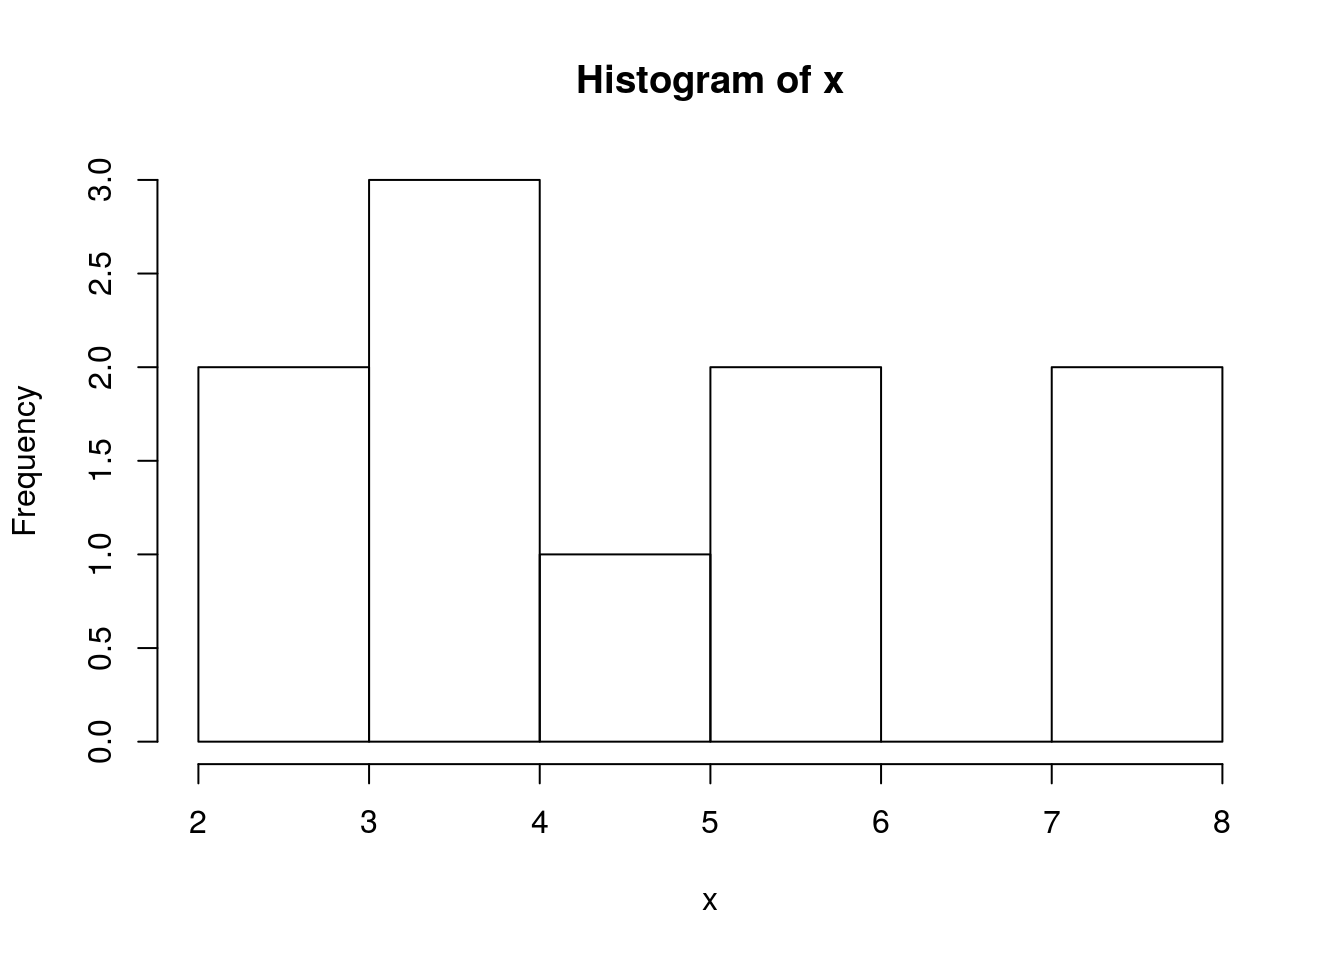
\includegraphics[width=0.5\linewidth]{Rcourse_files/figure-latex/unnamed-chunk-15-1}

R saves every object you create in RAM\footnote{S and S-Plus used to
  save objects on disk. Working from RAM has advantages and
  disadvantages. More on this in Chapter \ref{memory}.}. The collection
of all such objects is the \textbf{workspace} which you can inspect with

\begin{Shaded}
\begin{Highlighting}[]
\KeywordTok{ls}\NormalTok{()}
\end{Highlighting}
\end{Shaded}

\begin{verbatim}
## [1] "x"
\end{verbatim}

or with Ctrl+8 in RStudio.

If you lost your object, you can use \texttt{ls} with a text patter to
search for

\begin{Shaded}
\begin{Highlighting}[]
\KeywordTok{ls}\NormalTok{(}\DataTypeTok{pattern=}\StringTok{'x'}\NormalTok{)}
\end{Highlighting}
\end{Shaded}

\begin{verbatim}
## [1] "x"
\end{verbatim}

To remove objects from the workspace:

\begin{Shaded}
\begin{Highlighting}[]
\KeywordTok{rm}\NormalTok{(x) }\CommentTok{# remove variable}
\KeywordTok{ls}\NormalTok{() }\CommentTok{# verify}
\end{Highlighting}
\end{Shaded}

\begin{verbatim}
## character(0)
\end{verbatim}

You may think that if an object is removed then its memory is freed.
This is almost true, and depends on a negotiation mechanism between R
and the operating system. R's memory management is discussed in Chapter
\ref{memory}.

\section{Piping}\label{piping}

Because R originates in Unix and Linux environments, it inherits much of
its flavor.
\href{http://ryanstutorials.net/linuxtutorial/piping.php}{Piping} is an
idea take from the Linux shell which allows to use the output of one
expression as the input to another. Piping thus makes code easier to
read and write.

\BeginKnitrBlock{remark}
\iffalse {Remark. } \fi Volleyball fans may be confused with the idea of
spiking a ball from the 3-meter line, also called
\href{https://www.youtube.com/watch?v=GWW15Nr1lQM}{piping}. So: (a)
These are very different things. (b) If you can pipe,
\href{http://in.bgu.ac.il/sport/Pages/asa.aspx}{ASA-BGU} is looking for
you!
\EndKnitrBlock{remark}

Prerequisites:

\begin{Shaded}
\begin{Highlighting}[]
\KeywordTok{library}\NormalTok{(magrittr)}
\NormalTok{x <-}\StringTok{ }\KeywordTok{rbinom}\NormalTok{(}\DataTypeTok{n=}\DecValTok{1000}\NormalTok{, }\DataTypeTok{size=}\DecValTok{10}\NormalTok{, }\DataTypeTok{prob=}\FloatTok{0.5}\NormalTok{)}
\end{Highlighting}
\end{Shaded}

Examples

\begin{Shaded}
\begin{Highlighting}[]
\NormalTok{x %>%}\StringTok{ }\KeywordTok{var}\NormalTok{() }\CommentTok{# Instead of var(x)}
\NormalTok{x %>%}\StringTok{ }\KeywordTok{hist}\NormalTok{()  }\CommentTok{# Instead of hist(x)}
\NormalTok{x %>%}\StringTok{ }\KeywordTok{mean}\NormalTok{() %>%}\StringTok{ }\KeywordTok{round}\NormalTok{(}\DecValTok{2}\NormalTok{) %>%}\StringTok{ }\KeywordTok{add}\NormalTok{(}\DecValTok{10}\NormalTok{) }
\end{Highlighting}
\end{Shaded}

The next example\footnote{Taken from
  \url{http://cran.r-project.org/web/packages/magrittr/vignettes/magrittr.html}}
demonstrates the benefits of piping. The next two chunks of code do the
same thing. Try parsing them in your mind:

\begin{Shaded}
\begin{Highlighting}[]
\CommentTok{# Functional (onion) style}
\NormalTok{car_data <-}\StringTok{ }
\StringTok{  }\KeywordTok{transform}\NormalTok{(}\KeywordTok{aggregate}\NormalTok{(. ~}\StringTok{ }\NormalTok{cyl, }
                      \DataTypeTok{data =} \KeywordTok{subset}\NormalTok{(mtcars, hp >}\StringTok{ }\DecValTok{100}\NormalTok{), }
                      \DataTypeTok{FUN =} \NormalTok{function(x) }\KeywordTok{round}\NormalTok{(}\KeywordTok{mean}\NormalTok{(x, }\DecValTok{2}\NormalTok{))), }
            \DataTypeTok{kpl =} \NormalTok{mpg*}\FloatTok{0.4251}\NormalTok{)}
\end{Highlighting}
\end{Shaded}

\begin{Shaded}
\begin{Highlighting}[]
\CommentTok{# Piping (magrittr) style}
\NormalTok{car_data <-}\StringTok{ }
\StringTok{  }\NormalTok{mtcars %>%}
\StringTok{  }\KeywordTok{subset}\NormalTok{(hp >}\StringTok{ }\DecValTok{100}\NormalTok{) %>%}
\StringTok{  }\KeywordTok{aggregate}\NormalTok{(. ~}\StringTok{ }\NormalTok{cyl, }\DataTypeTok{data =} \NormalTok{., }\DataTypeTok{FUN =} \NormalTok{. %>%}\StringTok{ }\NormalTok{mean %>%}\StringTok{ }\KeywordTok{round}\NormalTok{(}\DecValTok{2}\NormalTok{)) %>%}
\StringTok{  }\KeywordTok{transform}\NormalTok{(}\DataTypeTok{kpl =} \NormalTok{mpg %>%}\StringTok{ }\KeywordTok{multiply_by}\NormalTok{(}\FloatTok{0.4251}\NormalTok{)) %>%}
\StringTok{  }\NormalTok{print}
\end{Highlighting}
\end{Shaded}

\section{Vector creation and
manipulation}\label{vector-creation-and-manipulation}

The most basic building block in R is the \textbf{vector}. We will now
see how to create them, and access their elements (i.e.~subsetting).
Here are three ways to create the same arbitrary vector:

\begin{Shaded}
\begin{Highlighting}[]
\KeywordTok{c}\NormalTok{(}\DecValTok{10}\NormalTok{, }\DecValTok{11}\NormalTok{, }\DecValTok{12}\NormalTok{, }\DecValTok{13}\NormalTok{, }\DecValTok{14}\NormalTok{, }\DecValTok{15}\NormalTok{, }\DecValTok{16}\NormalTok{, }\DecValTok{17}\NormalTok{, }\DecValTok{18}\NormalTok{, }\DecValTok{19}\NormalTok{, }\DecValTok{20}\NormalTok{, }\DecValTok{21}\NormalTok{) }\CommentTok{# manually}
\DecValTok{10}\NormalTok{:}\DecValTok{21} \CommentTok{# the `:` operator                            }
\KeywordTok{seq}\NormalTok{(}\DataTypeTok{from=}\DecValTok{10}\NormalTok{, }\DataTypeTok{to=}\DecValTok{21}\NormalTok{, }\DataTypeTok{by=}\DecValTok{1}\NormalTok{) }\CommentTok{# the seq() function}
\end{Highlighting}
\end{Shaded}

Lets assign it to the object named ``x'':

\begin{Shaded}
\begin{Highlighting}[]
\NormalTok{x <-}\StringTok{ }\KeywordTok{c}\NormalTok{(}\DecValTok{10}\NormalTok{, }\DecValTok{11}\NormalTok{, }\DecValTok{12}\NormalTok{, }\DecValTok{13}\NormalTok{, }\DecValTok{14}\NormalTok{, }\DecValTok{15}\NormalTok{, }\DecValTok{16}\NormalTok{, }\DecValTok{17}\NormalTok{, }\DecValTok{18}\NormalTok{, }\DecValTok{19}\NormalTok{, }\DecValTok{20}\NormalTok{, }\DecValTok{21}\NormalTok{)  }
\end{Highlighting}
\end{Shaded}

In the case you made a computation you do not want to repeat, you can
assign AFTER the computation is finished, since everything is saved by
the `.Last.value' variable.

\begin{Shaded}
\begin{Highlighting}[]
\KeywordTok{c}\NormalTok{(}\DecValTok{1}\NormalTok{,}\DecValTok{2}\NormalTok{,}\DecValTok{3}\NormalTok{)}
\NormalTok{y<-}\StringTok{ }\NormalTok{.Last.value }
\NormalTok{y}
\end{Highlighting}
\end{Shaded}

\begin{verbatim}
## [1] 1 2 3
## [1] "/home/johnros/workspace/Rcourse/docs/index.html"
\end{verbatim}

\BeginKnitrBlock{remark}
\iffalse {Remark. } \fi In line with the linux look and feel, variables
starting with a dot (.) are saved but are hidden. To show them see
\texttt{?ls}.
\EndKnitrBlock{remark}

Operations usually work element-wise:

\begin{Shaded}
\begin{Highlighting}[]
\NormalTok{x}\DecValTok{+2}
\end{Highlighting}
\end{Shaded}

\begin{verbatim}
##  [1] 12 13 14 15 16 17 18 19 20 21 22 23
\end{verbatim}

\begin{Shaded}
\begin{Highlighting}[]
\NormalTok{x*}\DecValTok{2}    
\end{Highlighting}
\end{Shaded}

\begin{verbatim}
##  [1] 20 22 24 26 28 30 32 34 36 38 40 42
\end{verbatim}

\begin{Shaded}
\begin{Highlighting}[]
\NormalTok{x^}\DecValTok{2}    
\end{Highlighting}
\end{Shaded}

\begin{verbatim}
##  [1] 100 121 144 169 196 225 256 289 324 361 400 441
\end{verbatim}

\begin{Shaded}
\begin{Highlighting}[]
\KeywordTok{sqrt}\NormalTok{(x)  }
\end{Highlighting}
\end{Shaded}

\begin{verbatim}
##  [1] 3.162278 3.316625 3.464102 3.605551 3.741657 3.872983 4.000000
##  [8] 4.123106 4.242641 4.358899 4.472136 4.582576
\end{verbatim}

\begin{Shaded}
\begin{Highlighting}[]
\KeywordTok{log}\NormalTok{(x)   }
\end{Highlighting}
\end{Shaded}

\begin{verbatim}
##  [1] 2.302585 2.397895 2.484907 2.564949 2.639057 2.708050 2.772589
##  [8] 2.833213 2.890372 2.944439 2.995732 3.044522
\end{verbatim}

\section{Search paths and packages}\label{search-paths-and-packages}

R can be easily extended with packages, which are merely a set of
functions and other objects, which can be loaded or unloaded at will.
Let's look at the function \texttt{sum}. We can see its contents by
calling it without arguments:

\begin{Shaded}
\begin{Highlighting}[]
\KeywordTok{print}\NormalTok{(read.csv)}
\end{Highlighting}
\end{Shaded}

\begin{verbatim}
## function (file, header = TRUE, sep = ",", quote = "\"", dec = ".", 
##     fill = TRUE, comment.char = "", ...) 
## read.table(file = file, header = header, sep = sep, quote = quote, 
##     dec = dec, fill = fill, comment.char = comment.char, ...)
## <bytecode: 0x4cec168>
## <environment: namespace:utils>
\end{verbatim}

Never mind what the function does. Note the
\texttt{environment:\ namespace:utils} line at the end. It tells us that
this function is part of the \textbf{utils} package. We did not need to
know this because it is loaded by default. Here are the packages that
are currently loaded:

\begin{Shaded}
\begin{Highlighting}[]
\KeywordTok{head}\NormalTok{(}\KeywordTok{search}\NormalTok{())}
\end{Highlighting}
\end{Shaded}

\begin{verbatim}
## [1] ".GlobalEnv"   "Penicillin"   "cases"        "Penicillin"  
## [5] "cases"        "package:grid"
\end{verbatim}

Other packages can be loaded via the \texttt{library} function, or
downloaded from the internet using the \texttt{install.packages}
function before loading with \texttt{library}. R's package import
mechanism is quite powerful, and is one of the reasons for R's success.

\section{Simple plotting}\label{simple-plotting}

R has many plotting facilities. We start with the simplest facilities,
namely, the \texttt{plot} function from the \textbf{graphics} package,
which is loaded by default.

\begin{Shaded}
\begin{Highlighting}[]
\NormalTok{x<-}\StringTok{ }\DecValTok{1}\NormalTok{:}\DecValTok{100}\NormalTok{; y<-}\StringTok{ }\DecValTok{3}\NormalTok{+}\KeywordTok{sin}\NormalTok{(x) }\CommentTok{# Create arbitrary data}
\KeywordTok{plot}\NormalTok{(}\DataTypeTok{x =} \NormalTok{x, }\DataTypeTok{y =} \NormalTok{y) }\CommentTok{# x,y syntax                         }
\end{Highlighting}
\end{Shaded}

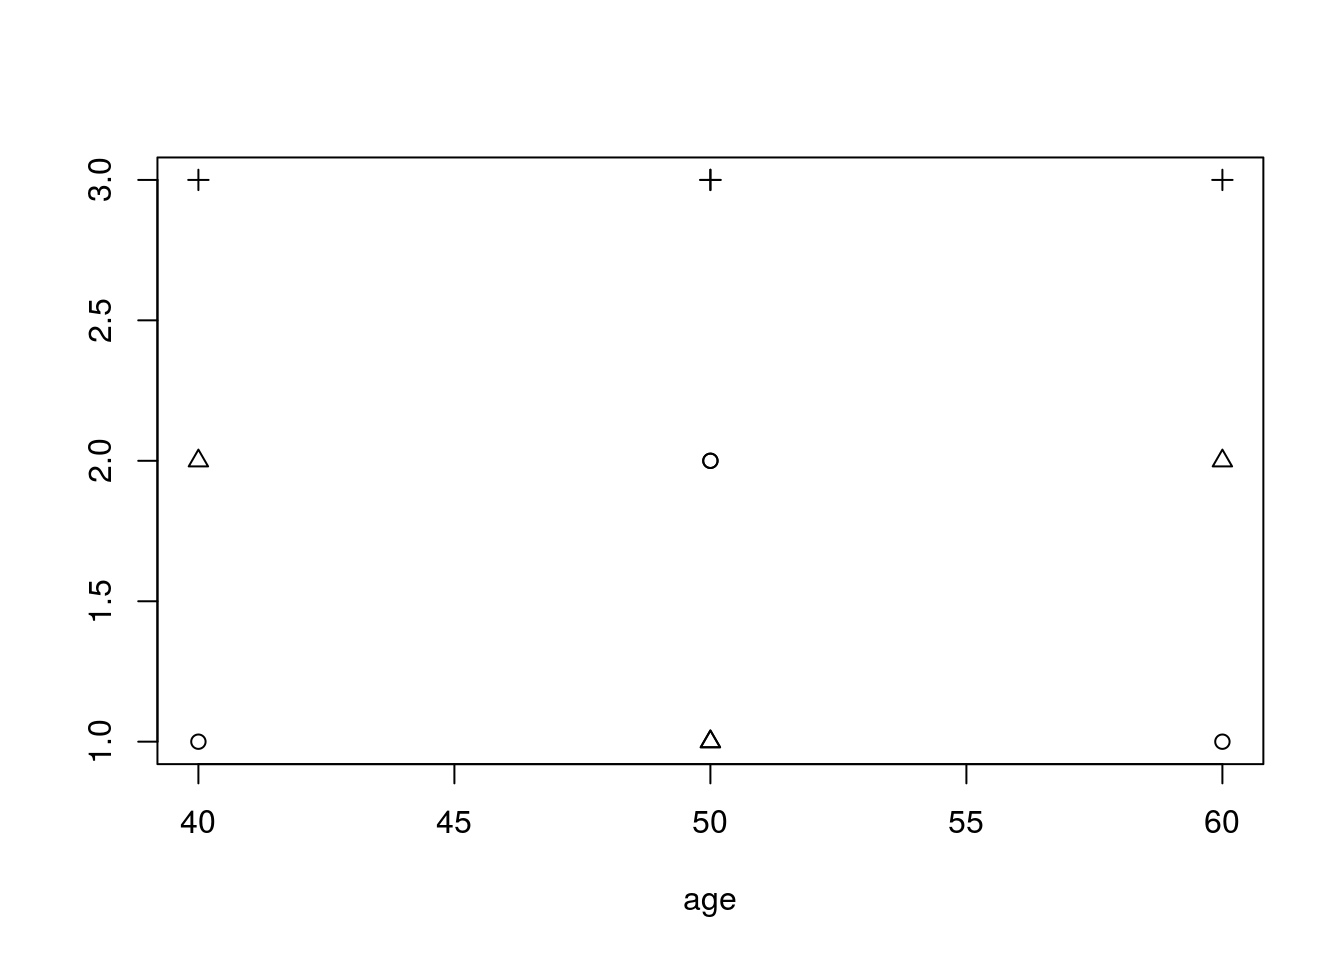
\includegraphics[width=0.5\linewidth]{Rcourse_files/figure-latex/unnamed-chunk-31-1}
Given an x argument and a y argument, \texttt{plot} tries to present a
scatter plot. We call this the ``x,y'' syntax. R has another, unique,
syntax to state functional relations. We call it the ``tilde'' syntax,
which originates in works of \citet{wilkinson1973symbolic}.

\begin{Shaded}
\begin{Highlighting}[]
\KeywordTok{plot}\NormalTok{(y ~}\StringTok{ }\NormalTok{x) }\CommentTok{# y~x syntax }
\end{Highlighting}
\end{Shaded}

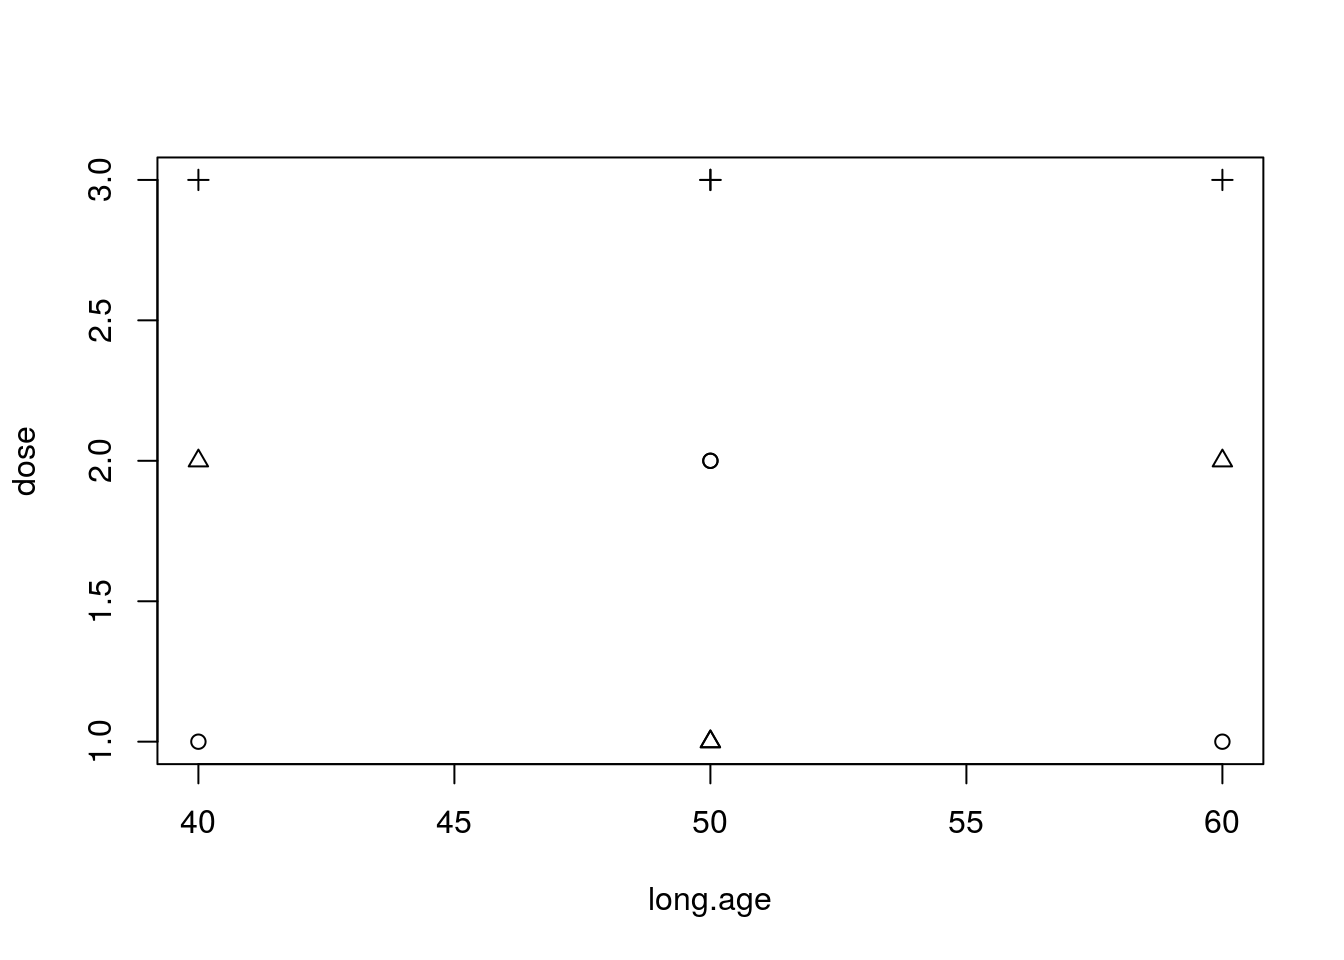
\includegraphics[width=0.5\linewidth]{Rcourse_files/figure-latex/unnamed-chunk-32-1}

The syntax \texttt{y\textasciitilde{}x} is read as ``y is a function of
x''. We will prefer the \texttt{y\textasciitilde{}x} syntax over the
\texttt{x,y} syntax since it is easier to read, and will be very useful
when we discuss more complicated models.

Here are some arguments that control the plot's appearance:

\begin{Shaded}
\begin{Highlighting}[]
\KeywordTok{plot}\NormalTok{(y~x, }\DataTypeTok{type=}\StringTok{'l'}\NormalTok{, }\DataTypeTok{main=}\StringTok{'Plotting a connected line'}\NormalTok{) }\CommentTok{# main title}
\end{Highlighting}
\end{Shaded}

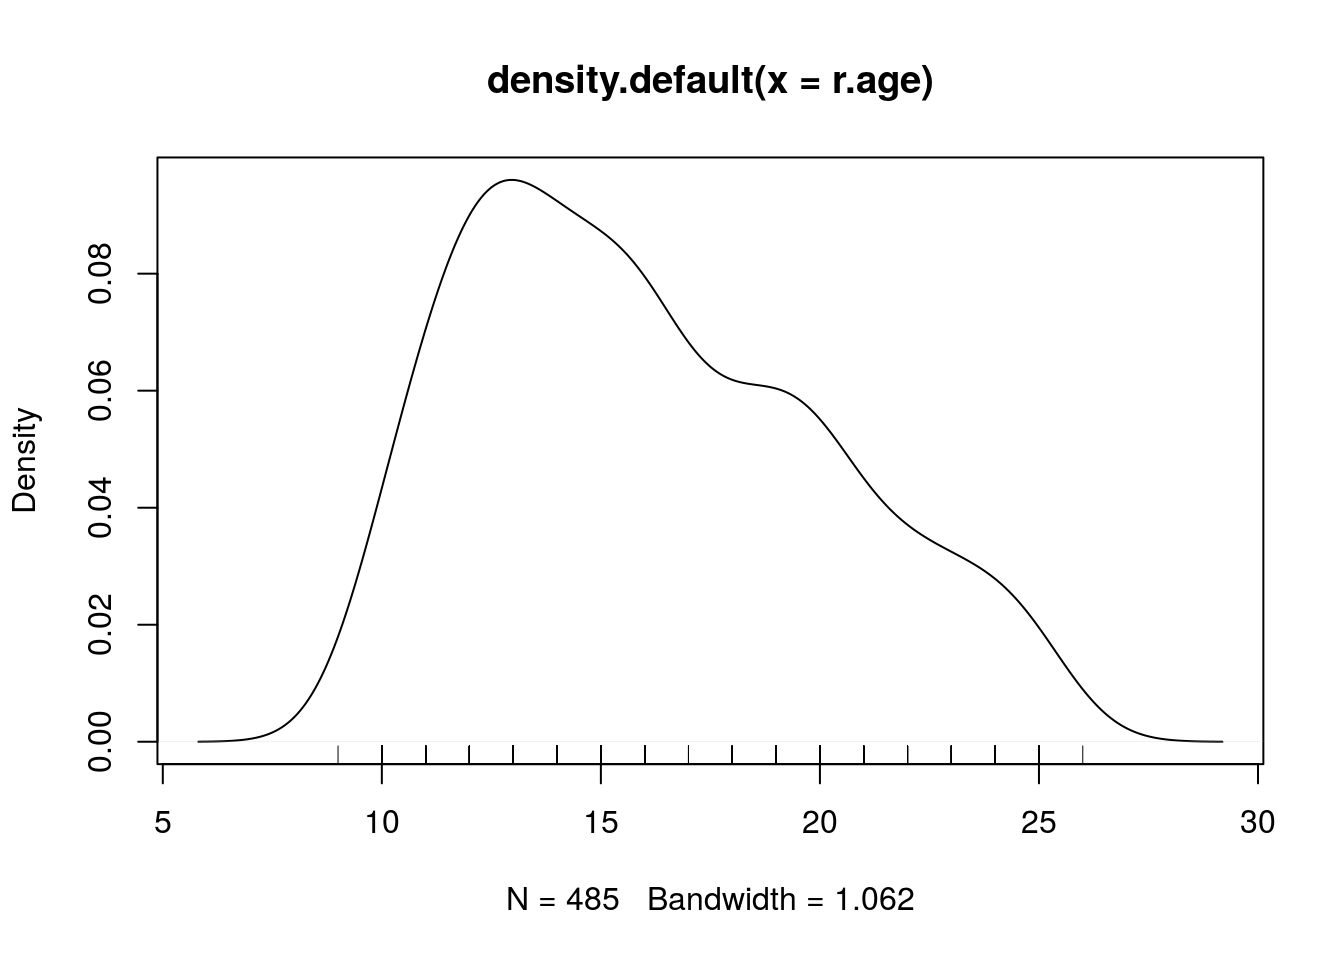
\includegraphics[width=0.5\linewidth]{Rcourse_files/figure-latex/unnamed-chunk-33-1}

\begin{Shaded}
\begin{Highlighting}[]
\KeywordTok{plot}\NormalTok{(y~x, }\DataTypeTok{type=}\StringTok{'h'}\NormalTok{, }\DataTypeTok{main=}\StringTok{'Sticks plot'}\NormalTok{, }\DataTypeTok{xlab=}\StringTok{'Insert x axis label'}\NormalTok{, }\DataTypeTok{ylab=}\StringTok{'Insert y axis label'}\NormalTok{) }\CommentTok{# axes labels}
\end{Highlighting}
\end{Shaded}

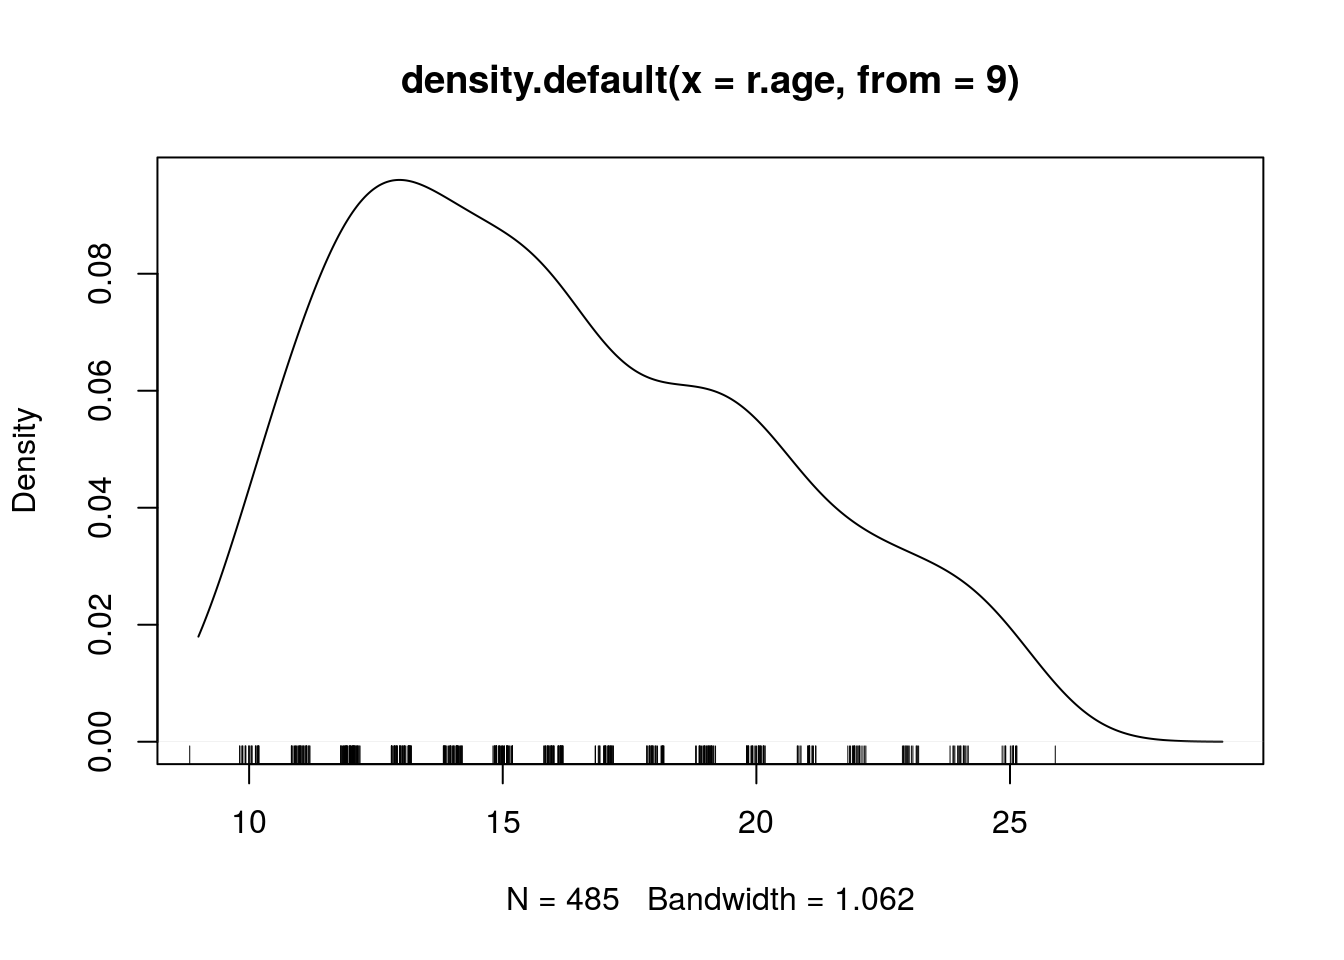
\includegraphics[width=0.5\linewidth]{Rcourse_files/figure-latex/unnamed-chunk-33-2}

\begin{Shaded}
\begin{Highlighting}[]
\KeywordTok{plot}\NormalTok{(y~x, }\DataTypeTok{pch=}\DecValTok{5}\NormalTok{) }\CommentTok{# Point type with pcf}
\end{Highlighting}
\end{Shaded}

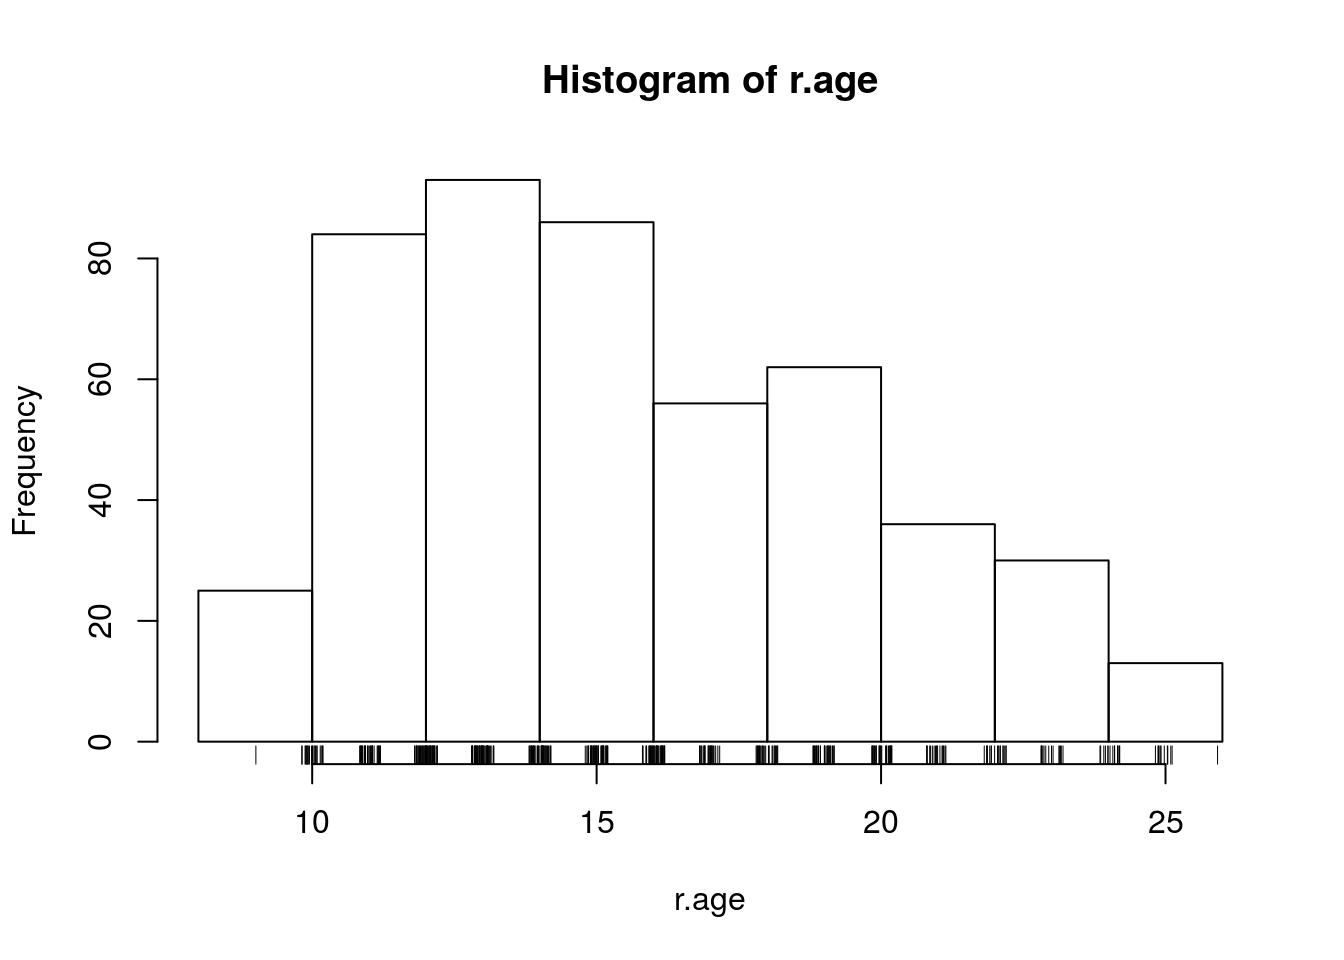
\includegraphics[width=0.5\linewidth]{Rcourse_files/figure-latex/unnamed-chunk-33-3}

\begin{Shaded}
\begin{Highlighting}[]
\KeywordTok{plot}\NormalTok{(y~x, }\DataTypeTok{pch=}\DecValTok{10}\NormalTok{, }\DataTypeTok{type=}\StringTok{'p'}\NormalTok{, }\DataTypeTok{col=}\StringTok{'blue'}\NormalTok{, }\DataTypeTok{cex=}\DecValTok{4}\NormalTok{) }\CommentTok{# More point parameters}
\KeywordTok{abline}\NormalTok{(}\DecValTok{3}\NormalTok{, }\FloatTok{0.002}\NormalTok{) }\CommentTok{# add linear line with slope b and intercept a}
\end{Highlighting}
\end{Shaded}

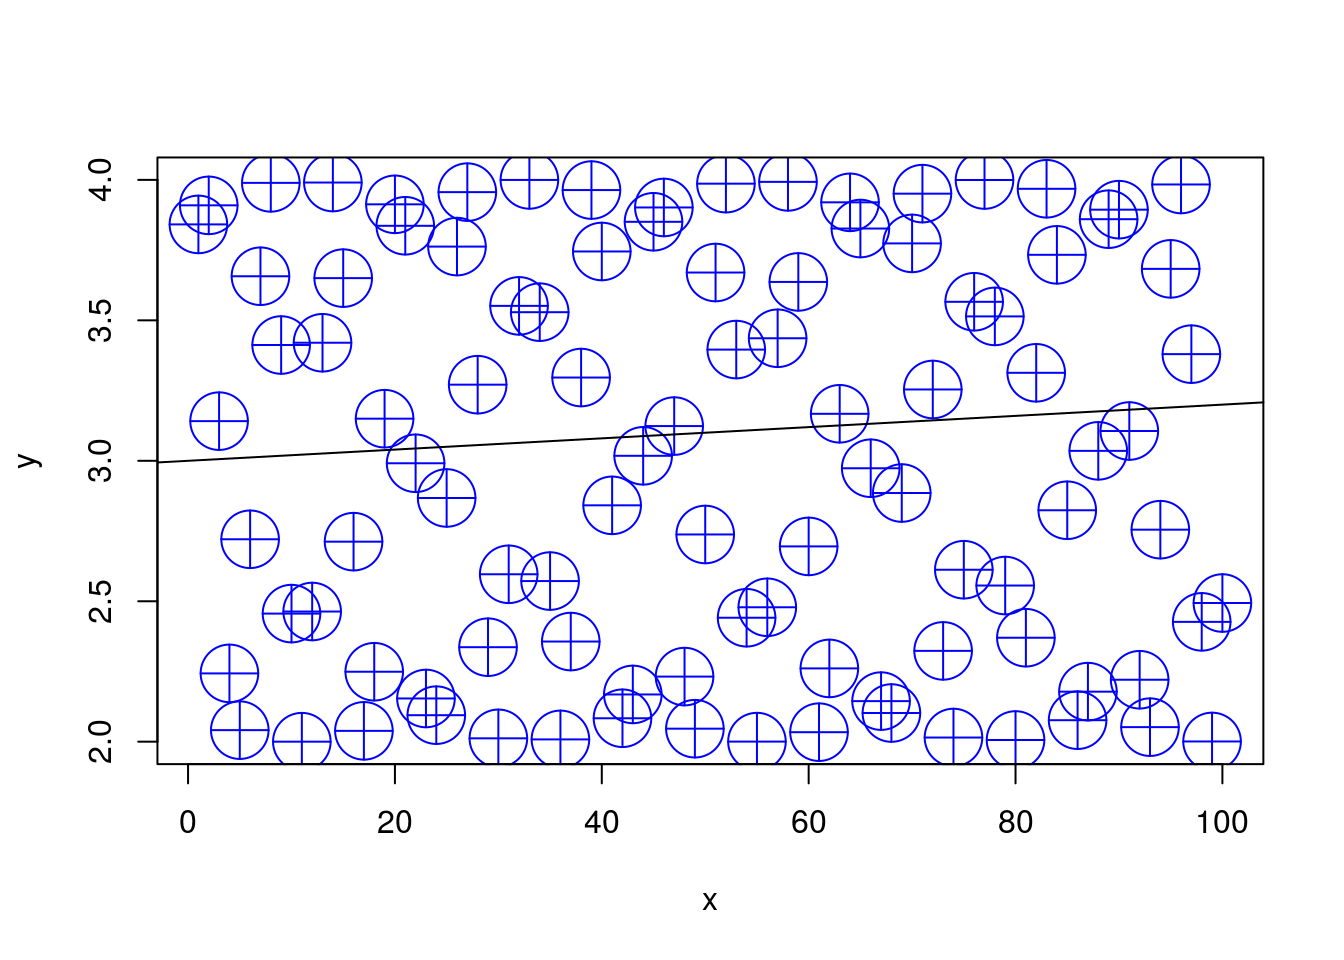
\includegraphics[width=0.5\linewidth]{Rcourse_files/figure-latex/unnamed-chunk-33-4}

For more plotting options run these

\begin{Shaded}
\begin{Highlighting}[]
\KeywordTok{example}\NormalTok{(plot)}
\KeywordTok{example}\NormalTok{(points)}
\NormalTok{?plot}
\KeywordTok{help}\NormalTok{(}\DataTypeTok{package=}\StringTok{'graphics'}\NormalTok{)}
\end{Highlighting}
\end{Shaded}

When your plotting gets serious, go to Chapter \ref{plotting}.

\section{Object types}\label{object-types}

We already saw that the basic building block of R objects is the vector.
Vectors can be of the following types:

\begin{itemize}
\tightlist
\item
  \textbf{character} Where each element is a string.
\item
  \textbf{numeric} Where each element is a ``real'' number in double
  precision floating point.
\item
  \textbf{integer} Where each element is an integer.
\item
  \textbf{logical} Where each element is either TRUE, FALSE, or
  NA\footnote{R uses a
    \href{https://en.wikipedia.org/wiki/Three-valued_logic}{three valued
    logic} where a missing value (NA) is neither TRUE, nor FALSE.}
\item
  \textbf{complex} Where each element is a complex number.
\item
  \textbf{list} Where each element is an arbitrary R object.
\item
  \textbf{factor} Factors are not actually vector objects, but they feel
  like such. They actually used to encode a finite set of values. This
  will be very useful when fitting linear model, but may be confusing if
  you think you are dealing with a character vector when in fact you are
  dealing with a factor. Be alert!
\end{itemize}

Vectors can be combined into larger objects. A \texttt{matrix} can be
thought of as the binding of several vectors of the same type. If
vectors of different types (but same length) are binded, we get a
\texttt{data\ frame} which is the most fundamental object in R for data
analysis.

\section{Data Frames}\label{data-frames}

Creating a simple data frame:

\begin{Shaded}
\begin{Highlighting}[]
\NormalTok{x<-}\StringTok{ }\DecValTok{1}\NormalTok{:}\DecValTok{10}
\NormalTok{y<-}\StringTok{ }\DecValTok{3} \NormalTok{+}\StringTok{ }\KeywordTok{sin}\NormalTok{(x) }
\NormalTok{frame1 <-}\StringTok{ }\KeywordTok{data.frame}\NormalTok{(}\DataTypeTok{x=}\NormalTok{x, }\DataTypeTok{sin=}\NormalTok{y)    }
\end{Highlighting}
\end{Shaded}

Lets inspect our data frame:

\begin{Shaded}
\begin{Highlighting}[]
\KeywordTok{head}\NormalTok{(frame1)}
\end{Highlighting}
\end{Shaded}

\begin{verbatim}
##   x      sin
## 1 1 3.841471
## 2 2 3.909297
## 3 3 3.141120
## 4 4 2.243198
## 5 5 2.041076
## 6 6 2.720585
\end{verbatim}

Now using the RStudio Excel-like viewer:

\begin{Shaded}
\begin{Highlighting}[]
\NormalTok{frame1 %>%}\StringTok{ }\KeywordTok{View}\NormalTok{() }
\end{Highlighting}
\end{Shaded}

We highly advise against editing the data this way since there will be
no documentation of the changes you made.

Verifying this is a data frame:

\begin{Shaded}
\begin{Highlighting}[]
\KeywordTok{class}\NormalTok{(frame1) }\CommentTok{# the object is of type data.frame}
\end{Highlighting}
\end{Shaded}

\begin{verbatim}
## [1] "data.frame"
\end{verbatim}

Check the dimension of the data

\begin{Shaded}
\begin{Highlighting}[]
\KeywordTok{dim}\NormalTok{(frame1)                             }
\end{Highlighting}
\end{Shaded}

\begin{verbatim}
## [1] 10  2
\end{verbatim}

Note that checking the dimension of a vector is different than checking
the dimension of a data frame.

\begin{Shaded}
\begin{Highlighting}[]
\KeywordTok{length}\NormalTok{(x)}
\end{Highlighting}
\end{Shaded}

\begin{verbatim}
## [1] 10
\end{verbatim}

A frame is a vector of column vectors, so its length is merely the
number of columns.

\begin{Shaded}
\begin{Highlighting}[]
\KeywordTok{length}\NormalTok{(frame1) }
\end{Highlighting}
\end{Shaded}

\begin{verbatim}
## [1] 2
\end{verbatim}

\section{Exctraction}\label{exctraction}

R provides many ways to subset and extract elements from vectors and
other objects. The basics are fairly simple, but not paying attention to
the ``personality'' of each extraction mechanism may cause you a lot of
headache.

For starters, extraction is done with the \texttt{{[}} operator. The
operator can take vectors of all types.

Extracting element with by integer index:

\begin{Shaded}
\begin{Highlighting}[]
\NormalTok{frame1[}\DecValTok{1}\NormalTok{, }\DecValTok{2}\NormalTok{]  }\CommentTok{# exctract the element in the 1st row and 2nd column.}
\end{Highlighting}
\end{Shaded}

\begin{verbatim}
## [1] 3.841471
\end{verbatim}

Extract \textbf{column} by index:

\begin{Shaded}
\begin{Highlighting}[]
\NormalTok{frame1[}\DecValTok{1}\NormalTok{, ]                             }
\end{Highlighting}
\end{Shaded}

\begin{verbatim}
##   x      sin
## 1 1 3.841471
\end{verbatim}

Extract column by name:

\begin{Shaded}
\begin{Highlighting}[]
\NormalTok{frame1[, }\StringTok{'sin'}\NormalTok{]}
\end{Highlighting}
\end{Shaded}

\begin{verbatim}
##  [1] 3.841471 3.909297 3.141120 2.243198 2.041076 2.720585 3.656987
##  [8] 3.989358 3.412118 2.455979
\end{verbatim}

What did we just extract?

\begin{Shaded}
\begin{Highlighting}[]
\KeywordTok{dim}\NormalTok{(frame1[, }\StringTok{'sin'}\NormalTok{])  }\CommentTok{# extracts a column vector}
\end{Highlighting}
\end{Shaded}

\begin{verbatim}
## NULL
\end{verbatim}

\begin{Shaded}
\begin{Highlighting}[]
\KeywordTok{dim}\NormalTok{(frame1[}\StringTok{'sin'}\NormalTok{])  }\CommentTok{# extracts a data frame}
\end{Highlighting}
\end{Shaded}

\begin{verbatim}
## [1] 10  1
\end{verbatim}

\begin{Shaded}
\begin{Highlighting}[]
\KeywordTok{dim}\NormalTok{(frame1[,}\DecValTok{1}\NormalTok{:}\DecValTok{2}\NormalTok{])  }\CommentTok{# extracts a data frame}
\end{Highlighting}
\end{Shaded}

\begin{verbatim}
## [1] 10  2
\end{verbatim}

\begin{Shaded}
\begin{Highlighting}[]
\KeywordTok{dim}\NormalTok{(frame1[}\DecValTok{2}\NormalTok{])  }\CommentTok{# extracts a data frame}
\end{Highlighting}
\end{Shaded}

\begin{verbatim}
## [1] 10  1
\end{verbatim}

\begin{Shaded}
\begin{Highlighting}[]
\KeywordTok{dim}\NormalTok{(frame1[}\DecValTok{2}\NormalTok{, ])  }\CommentTok{# extract a data frame}
\end{Highlighting}
\end{Shaded}

\begin{verbatim}
## [1] 1 2
\end{verbatim}

\begin{Shaded}
\begin{Highlighting}[]
\KeywordTok{dim}\NormalTok{(frame1$sin)  }\CommentTok{# extracts a column vector}
\end{Highlighting}
\end{Shaded}

\begin{verbatim}
## NULL
\end{verbatim}

The \texttt{subset()} function does the same

\begin{Shaded}
\begin{Highlighting}[]
\KeywordTok{subset}\NormalTok{(frame1, }\DataTypeTok{select=}\NormalTok{sin) }
\KeywordTok{subset}\NormalTok{(frame1, }\DataTypeTok{select=}\DecValTok{2}\NormalTok{)}
\KeywordTok{subset}\NormalTok{(frame1, }\DataTypeTok{select=} \KeywordTok{c}\NormalTok{(}\DecValTok{2}\NormalTok{,}\DecValTok{0}\NormalTok{))}
\end{Highlighting}
\end{Shaded}

If you are unsatisfied with the output of the \texttt{{[}} mechanism,
you can use \texttt{{[}{[}}, which gets the content of a vector, while
stripping the attributes.

\begin{Shaded}
\begin{Highlighting}[]
\NormalTok{a <-}\StringTok{ }\NormalTok{frame1[}\DecValTok{1}\NormalTok{] }\CommentTok{# [ extraction}
\NormalTok{b <-}\StringTok{ }\NormalTok{frame1[[}\DecValTok{1}\NormalTok{]] }\CommentTok{# [[ extraction}
\NormalTok{a==b }\CommentTok{# objects are element-wise identical }
\end{Highlighting}
\end{Shaded}

\begin{verbatim}
##          x
##  [1,] TRUE
##  [2,] TRUE
##  [3,] TRUE
##  [4,] TRUE
##  [5,] TRUE
##  [6,] TRUE
##  [7,] TRUE
##  [8,] TRUE
##  [9,] TRUE
## [10,] TRUE
\end{verbatim}

\begin{Shaded}
\begin{Highlighting}[]
\KeywordTok{class}\NormalTok{(a)==}\KeywordTok{class}\NormalTok{(b)}
\end{Highlighting}
\end{Shaded}

\begin{verbatim}
## [1] FALSE
\end{verbatim}

The different types of output causes different behaviors

\begin{Shaded}
\begin{Highlighting}[]
\NormalTok{a[}\DecValTok{1}\NormalTok{]}
\end{Highlighting}
\end{Shaded}

\begin{verbatim}
##     x
## 1   1
## 2   2
## 3   3
## 4   4
## 5   5
## 6   6
## 7   7
## 8   8
## 9   9
## 10 10
\end{verbatim}

\begin{Shaded}
\begin{Highlighting}[]
\NormalTok{b[}\DecValTok{1}\NormalTok{]}
\end{Highlighting}
\end{Shaded}

\begin{verbatim}
## [1] 1
\end{verbatim}

If you want to learn more about subsetting see
\href{http://adv-r.had.co.nz/Subsetting.html}{Hadley's guide}, and our
Chapter \ref{hadley}

\section{Data Import and Export}\label{data-import-and-export}

For any practical purpose, you will not be generating your data
manually. R comes with many importing and exporting mechanism which we
now present. If, however, you do a lot of data ``munging'', make sure to
see Hadley-verse Chapter \ref{hadley}. If you work with MASSIVE data
sets, read about the \textbf{data.table} package. For a complete review
see the \href{http://cran.r-project.org/doc/manuals/R-data.html}{R
manual}.

\subsection{Import from WEB}\label{import-from-web}

The \texttt{read.table} function is the main importing workhorse. It can
import directly from the web.

\begin{Shaded}
\begin{Highlighting}[]
\NormalTok{URL <-}\StringTok{ 'http://statweb.stanford.edu/~tibs/ElemStatLearn/datasets/bone.data'}
\NormalTok{tirgul1 <-}\StringTok{ }\KeywordTok{read.table}\NormalTok{(URL)}
\end{Highlighting}
\end{Shaded}

Always look at the imported result!

\begin{Shaded}
\begin{Highlighting}[]
\KeywordTok{head}\NormalTok{(tirgul1)}
\end{Highlighting}
\end{Shaded}

\begin{verbatim}
##      V1    V2     V3          V4
## 1 idnum   age gender      spnbmd
## 2     1  11.7   male  0.01808067
## 3     1  12.7   male  0.06010929
## 4     1 13.75   male 0.005857545
## 5     2 13.25   male  0.01026393
## 6     2  14.3   male   0.2105263
\end{verbatim}

Ohh dear. The header row was not recognized. Fix with
\texttt{header=TRUE}:

\begin{Shaded}
\begin{Highlighting}[]
\NormalTok{tirgul1 <-}\StringTok{ }\KeywordTok{read.table}\NormalTok{(URL, }\DataTypeTok{header =} \OtherTok{TRUE}\NormalTok{) }
\KeywordTok{head}\NormalTok{(tirgul1)}
\end{Highlighting}
\end{Shaded}

\subsection{Export as CSV}\label{export-as-csv}

Let's write a simple file so that we have something to import

\begin{Shaded}
\begin{Highlighting}[]
\KeywordTok{head}\NormalTok{(airquality) }\CommentTok{#  examine the data to export}
\end{Highlighting}
\end{Shaded}

\begin{verbatim}
##   Ozone Solar.R Wind Temp Month Day
## 1    41     190  7.4   67     5   1
## 2    36     118  8.0   72     5   2
## 3    12     149 12.6   74     5   3
## 4    18     313 11.5   62     5   4
## 5    NA      NA 14.3   56     5   5
## 6    28      NA 14.9   66     5   6
\end{verbatim}

\begin{Shaded}
\begin{Highlighting}[]
\NormalTok{temp.file.name <-}\StringTok{ }\KeywordTok{tempfile}\NormalTok{() }\CommentTok{# get some arbitrary file name}
\KeywordTok{write.csv}\NormalTok{(}\DataTypeTok{x =} \NormalTok{airquality, }\DataTypeTok{file =} \NormalTok{temp.file.name) }\CommentTok{# export}
\end{Highlighting}
\end{Shaded}

Now let's import the exported file. Being a .csv file, I can use
\texttt{read.csv} instead of \texttt{read.table}.

\begin{Shaded}
\begin{Highlighting}[]
\NormalTok{my.data<-}\StringTok{ }\KeywordTok{read.csv}\NormalTok{(}\DataTypeTok{file=}\NormalTok{temp.file.name) }\CommentTok{# import}
\KeywordTok{head}\NormalTok{(my.data) }\CommentTok{# verify import}
\end{Highlighting}
\end{Shaded}

\begin{verbatim}
##   X Ozone Solar.R Wind Temp Month Day
## 1 1    41     190  7.4   67     5   1
## 2 2    36     118  8.0   72     5   2
## 3 3    12     149 12.6   74     5   3
## 4 4    18     313 11.5   62     5   4
## 5 5    NA      NA 14.3   56     5   5
## 6 6    28      NA 14.9   66     5   6
\end{verbatim}

\BeginKnitrBlock{remark}
\iffalse {Remark. } \fi Windows users may need to use
``\textbackslash{}'' instead of ``/''.
\EndKnitrBlock{remark}

\subsection{Reading From Text Files}\label{reading-from-text-files}

Some general notes on importing text files via the \texttt{read.table}
function. But first, we need to know what is the active directory. Here
is how to get and set R's active directory:

\begin{Shaded}
\begin{Highlighting}[]
\KeywordTok{getwd}\NormalTok{() }\CommentTok{#What is the working directory?}
\KeywordTok{setwd}\NormalTok{() }\CommentTok{#Setting the working directory in Linux}
\end{Highlighting}
\end{Shaded}

We can now call the \texttt{read.table} function to import text files.
If you care about your sanity, see \texttt{?read.table} before starting
imports. Some notable properties of the function:

\begin{itemize}
\tightlist
\item
  \texttt{read.table} will try to guess column separators (tab, comma,
  etc.)
\item
  \texttt{read.table} will try to guess if a header row is present.
\item
  \texttt{read.table} will convert character vectors to factors unless
  told not to.
\item
  The output of \texttt{read.table} needs to be explicitly assigned to
  an object for it to be saved.
\end{itemize}

\subsection{Writing Data to Text
Files}\label{writing-data-to-text-files}

The function \texttt{write.table} is the exporting counterpart of
\texttt{read.table}.

\subsection{.XLS(X) files}\label{xlsx-files}

Strongly recommended to convert to .csv in Excel, and then import as
csv. If you still insist see
\href{http://cran.r-project.org/doc/manuals/R-data.html\#Reading-Excel-spreadsheets}{here}.

\subsection{Massive files}\label{massive-files}

The above importing and exporting mechanism were not designed for
massive files. See the section on Sparse Representation (\ref{sparse})
and Out-of-Ram Algorithms (\ref{memory}) for more on working with
massive data files.

\subsection{Databases}\label{databases}

R can does not need to read from text files; it can read directly from a
data base. This is very useful since it allows the filtering, selecting
and joining operations to rely on the database's optimized algorithms.
See
\href{https://rforanalytics.wordpress.com/useful-links-for-r/odbc-databases-for-r/}{here}.

\section{Functions}\label{functions}

One of the most basic building blocks of programming is the ability of
writing your own functions. A function in R, like everything else, is a
an object accessible using its name. We first define a simple function
that sums its two arguments

\begin{Shaded}
\begin{Highlighting}[]
\NormalTok{my.sum <-}\StringTok{ }\NormalTok{function(x,y) \{}
  \NormalTok{x+y}
\NormalTok{\}}
\KeywordTok{my.sum}\NormalTok{(}\DecValTok{10}\NormalTok{,}\DecValTok{2}\NormalTok{)}
\end{Highlighting}
\end{Shaded}

\begin{verbatim}
## [1] 12
\end{verbatim}

From this example you may notice that:

\begin{itemize}
\tightlist
\item
  The function \texttt{function} tells R to construct a function object.
\item
  The arguments of the \texttt{function}, i.e. \texttt{(x,y)}, need to
  be named but we are not required to specify their type.
\item
  A typical R function does not change objects\footnote{This is a
    classical \emph{functional programming} paradigm. If you are used to
    \emph{object oriented} programming, you may want to read about
    \href{http://adv-r.had.co.nz/R5.html}{references classes} which may
    be required if you are planning to compute with very complicated
    objects.} but rather creates new ones. To save the output pf
  \texttt{my.sum} we will need to assign it using the
  \texttt{\textless{}-} operator.
\item
  The function will output its last evaluated expression.
\end{itemize}

\section{Looping}\label{looping}

The real power of scripting is when repeated operations are done by
iteration. R supports the usual \texttt{for}, \texttt{while}, and
\texttt{repated} loops. Here is an embarrassingly simple example

\begin{Shaded}
\begin{Highlighting}[]
\NormalTok{for (i in }\DecValTok{1}\NormalTok{:}\DecValTok{5}\NormalTok{)\{}
    \KeywordTok{print}\NormalTok{(i)}
    \NormalTok{\}}
\end{Highlighting}
\end{Shaded}

\begin{verbatim}
## [1] 1
## [1] 2
## [1] 3
## [1] 4
## [1] 5
\end{verbatim}

\section{Recursion}\label{recursion}

The R compiler is really not designed for recursion, and you will rarely
need to do so.\\
See the RCpp Chapter \ref{rcpp} for linking C code, which is better
suited for recursion. If you really insist to write recursions in R,
make sure to use the \texttt{Recall} function, as this Fibonacci series
example demonstrates.

\begin{Shaded}
\begin{Highlighting}[]
\NormalTok{fib<-function(n) \{}
    \NormalTok{if (n <}\StringTok{ }\DecValTok{2}\NormalTok{) fn<-}\DecValTok{1} 
    \NormalTok{else fn<-}\KeywordTok{Recall}\NormalTok{(n -}\StringTok{ }\DecValTok{1}\NormalTok{) +}\StringTok{ }\KeywordTok{Recall}\NormalTok{(n -}\StringTok{ }\DecValTok{2}\NormalTok{) }
    \KeywordTok{return}\NormalTok{(fn)}
\NormalTok{\} }
\KeywordTok{fib}\NormalTok{(}\DecValTok{5}\NormalTok{)}
\end{Highlighting}
\end{Shaded}

\begin{verbatim}
## [1] 8
\end{verbatim}

\section{Bibliographic Notes}\label{bibliographic-notes-1}

There are endlessly many introductory texts on R. For a list of free
resources see
\href{http://stats.stackexchange.com/questions/138/free-resources-for-learning-r}{CrossValidated}.
I personally recommend the official introduction
\citet{venables2004introduction}, or anything else Bill Venables writes.
For advanced R programming see \citet{wickham2014advanced}, or anything
else Hadley Wickham writes.

\chapter{Exploratory Data Analysis}\label{eda}

Exploratory Data Analysis (EDA) is a term cast by
\href{https://en.wikipedia.org/wiki/John_Tukey}{John W. Tukey} in his
seminal book \citet{tukey1977exploratory}. It is the practice of
inspecting, exploring your data before stating hypotheses, fitting
predictors, and other more ambitious inferential goals. It typically
includes the computation of simple \emph{summary statistics} which
capture some property of interest in the data, and \emph{visualization}.
EDA can be thought of as an assumption free, purely algorithmic
practice.

In this text we present EDA techniques along the following lines:

\begin{itemize}
\tightlist
\item
  How we explore: with a summary statistic or visually.
\item
  How many variable analyzed simultaneously: univariate, bivariate, or
  multivariate.
\item
  What type of variable: categorical or continuous.
\end{itemize}

\section{Summary Statistics}\label{summary-statistics}

\subsection{Categorical Data}\label{categorical-data}

Categorical variable do not admit any mathematical operations on them.
We cannot sum them, or even sort them. We can only \textbf{count} them.
As such, summaries of categorical variables will always start with the
counting of the frequency of each category.

\subsubsection{Summary of Univariate Categorical
Data}\label{summary-of-univariate-categorical-data}

\begin{Shaded}
\begin{Highlighting}[]
\NormalTok{gender <-}\StringTok{ }\KeywordTok{c}\NormalTok{(}\KeywordTok{rep}\NormalTok{(}\StringTok{'Boy'}\NormalTok{, }\DecValTok{10}\NormalTok{), }\KeywordTok{rep}\NormalTok{(}\StringTok{'Girl'}\NormalTok{, }\DecValTok{12}\NormalTok{))}
\NormalTok{drink <-}\StringTok{ }\KeywordTok{c}\NormalTok{(}\KeywordTok{rep}\NormalTok{(}\StringTok{'Coke'}\NormalTok{, }\DecValTok{5}\NormalTok{), }\KeywordTok{rep}\NormalTok{(}\StringTok{'Sprite'}\NormalTok{, }\DecValTok{3}\NormalTok{), }\KeywordTok{rep}\NormalTok{(}\StringTok{'Coffee'}\NormalTok{, }\DecValTok{6}\NormalTok{), }\KeywordTok{rep}\NormalTok{(}\StringTok{'Tea'}\NormalTok{, }\DecValTok{7}\NormalTok{), }\KeywordTok{rep}\NormalTok{(}\StringTok{'Water'}\NormalTok{, }\DecValTok{1}\NormalTok{))  }
\NormalTok{age <-}\StringTok{  }\KeywordTok{sample}\NormalTok{(}\KeywordTok{c}\NormalTok{(}\StringTok{'Young'}\NormalTok{, }\StringTok{'Old'}\NormalTok{), }\DataTypeTok{size =} \KeywordTok{length}\NormalTok{(gender), }\DataTypeTok{replace =} \OtherTok{TRUE}\NormalTok{)}

\KeywordTok{table}\NormalTok{(gender)}
\end{Highlighting}
\end{Shaded}

\begin{verbatim}
## gender
##  Boy Girl 
##   10   12
\end{verbatim}

\begin{Shaded}
\begin{Highlighting}[]
\KeywordTok{table}\NormalTok{(drink)}
\end{Highlighting}
\end{Shaded}

\begin{verbatim}
## drink
## Coffee   Coke Sprite    Tea  Water 
##      6      5      3      7      1
\end{verbatim}

\begin{Shaded}
\begin{Highlighting}[]
\KeywordTok{table}\NormalTok{(age)}
\end{Highlighting}
\end{Shaded}

\begin{verbatim}
## age
##   Old Young 
##    11    11
\end{verbatim}

If instead of the level counts you want the proportions, you can use
\texttt{prop.table}

\begin{Shaded}
\begin{Highlighting}[]
\KeywordTok{prop.table}\NormalTok{(}\KeywordTok{table}\NormalTok{(gender))}
\end{Highlighting}
\end{Shaded}

\begin{verbatim}
## gender
##       Boy      Girl 
## 0.4545455 0.5454545
\end{verbatim}

\subsubsection{Summary of Bivariate Categorical
Data}\label{summary-of-bivariate-categorical-data}

\begin{Shaded}
\begin{Highlighting}[]
\KeywordTok{library}\NormalTok{(magrittr)}
\KeywordTok{cbind}\NormalTok{(gender, drink) %>%}\StringTok{ }\NormalTok{head }\CommentTok{# inspect the raw data}
\end{Highlighting}
\end{Shaded}

\begin{verbatim}
##      gender drink   
## [1,] "Boy"  "Coke"  
## [2,] "Boy"  "Coke"  
## [3,] "Boy"  "Coke"  
## [4,] "Boy"  "Coke"  
## [5,] "Boy"  "Coke"  
## [6,] "Boy"  "Sprite"
\end{verbatim}

\begin{Shaded}
\begin{Highlighting}[]
\NormalTok{table1 <-}\StringTok{ }\KeywordTok{table}\NormalTok{(gender, drink) }
\NormalTok{table1                                      }
\end{Highlighting}
\end{Shaded}

\begin{verbatim}
##       drink
## gender Coffee Coke Sprite Tea Water
##   Boy       2    5      3   0     0
##   Girl      4    0      0   7     1
\end{verbatim}

\subsubsection{Summary of Multivariate Categorical
Data}\label{summary-of-multivariate-categorical-data}

You may be wondering how does R handle tables with more than two
dimensions. It is indeed not trivial, and R offers several solutions.

\begin{Shaded}
\begin{Highlighting}[]
\NormalTok{table2}\FloatTok{.1} \NormalTok{<-}\StringTok{ }\KeywordTok{table}\NormalTok{(gender, drink, age) }\CommentTok{# A multilevel table. }
\NormalTok{table2}\FloatTok{.1}
\end{Highlighting}
\end{Shaded}

\begin{verbatim}
## , , age = Old
## 
##       drink
## gender Coffee Coke Sprite Tea Water
##   Boy       0    2      2   0     0
##   Girl      4    0      0   2     1
## 
## , , age = Young
## 
##       drink
## gender Coffee Coke Sprite Tea Water
##   Boy       2    3      1   0     0
##   Girl      0    0      0   5     0
\end{verbatim}

\begin{Shaded}
\begin{Highlighting}[]
\NormalTok{table}\FloatTok{.2.2} \NormalTok{<-}\StringTok{ }\KeywordTok{ftable}\NormalTok{(gender, drink, age) }\CommentTok{# A human readable table.}
\NormalTok{table}\FloatTok{.2.2}
\end{Highlighting}
\end{Shaded}

\begin{verbatim}
##               age Old Young
## gender drink               
## Boy    Coffee       0     2
##        Coke         2     3
##        Sprite       2     1
##        Tea          0     0
##        Water        0     0
## Girl   Coffee       4     0
##        Coke         0     0
##        Sprite       0     0
##        Tea          2     5
##        Water        1     0
\end{verbatim}

If you want proportions instead of counts, you need to specify the
denominator, i.e., the margins.

\begin{Shaded}
\begin{Highlighting}[]
\KeywordTok{prop.table}\NormalTok{(table1, }\DataTypeTok{margin =} \DecValTok{1}\NormalTok{)}
\end{Highlighting}
\end{Shaded}

\begin{verbatim}
##       drink
## gender     Coffee       Coke     Sprite        Tea      Water
##   Boy  0.20000000 0.50000000 0.30000000 0.00000000 0.00000000
##   Girl 0.33333333 0.00000000 0.00000000 0.58333333 0.08333333
\end{verbatim}

\begin{Shaded}
\begin{Highlighting}[]
\KeywordTok{prop.table}\NormalTok{(table1, }\DataTypeTok{margin =} \DecValTok{2}\NormalTok{)}
\end{Highlighting}
\end{Shaded}

\begin{verbatim}
##       drink
## gender    Coffee      Coke    Sprite       Tea     Water
##   Boy  0.3333333 1.0000000 1.0000000 0.0000000 0.0000000
##   Girl 0.6666667 0.0000000 0.0000000 1.0000000 1.0000000
\end{verbatim}

\subsection{Continous Data}\label{continous-data}

Continuous variables admit many more operations than categorical. We can
thus compute sums, means, quantiles, and more.

\subsubsection{Summary of Univariate Continous
Data}\label{summary-of-univariate-continous-data}

We distinguish between several types of summaries, each capturing a
different property of the data.

\subsubsection{Summary of Location}\label{summary-of-location}

Capture the ``location'' of the data. These include:

\BeginKnitrBlock{definition}
\protect\hypertarget{def:unnamed-chunk-64}{}{\label{def:unnamed-chunk-64}}The
mean, or average, of a sample \(x\) of lenth \(n\), denoted \(\bar x\)
is defined as \[ \bar x := n^{-1} \sum x_i \]
\EndKnitrBlock{definition}

The sample mean is \textbf{non robust}. A single large observation may
inflate the mean indefinitely. For this reason, we define several other
summaries of location, which are more robust, i.e., less affected by
``contaminations'' of the data.

We start by defining the sample quantiles, themselves \textbf{not} a
summary of location.

\BeginKnitrBlock{definition}
\protect\hypertarget{def:unnamed-chunk-65}{}{\label{def:unnamed-chunk-65}}The
\(\alpha\) quantile of a sample \(x\), denoted \(x_\alpha\), is (non
uniquely) defined as a value above \(100 \alpha \%\) of the sample, and
below \(100 (1-\alpha) \%\).
\EndKnitrBlock{definition}

We emphasize that sample quantiles are non-uniquely defined. See
\texttt{?quantile} for the 9(!) different definitions that R provides.

We can now define another summary of location, the median.

\BeginKnitrBlock{definition}
\protect\hypertarget{def:unnamed-chunk-66}{}{\label{def:unnamed-chunk-66}}The
median of a sample \(x\), denoted \(x_{0.5}\) is the \(\alpha=0.5\)
quantile of the sample.
\EndKnitrBlock{definition}

A whole family of summaries of locations is the \textbf{alpha trimmed
mean}.

\BeginKnitrBlock{definition}
\protect\hypertarget{def:unnamed-chunk-67}{}{\label{def:unnamed-chunk-67}}The
\(\alpha\) trimmed mean of a sample \(x\), denoted \(\bar x_\alpha\) is
the average of the sample after removing the \(\alpha\) largest and
\(\alpha\) smallest observations.
\EndKnitrBlock{definition}

The simple mean and median are instances of the alpha trimmed mean:
\(\bar x_0\) and \(\bar x_{0.5}\) respectively.

Here are the R implementations:

\begin{Shaded}
\begin{Highlighting}[]
\NormalTok{x <-}\StringTok{ }\KeywordTok{rexp}\NormalTok{(}\DecValTok{100}\NormalTok{)}
\KeywordTok{mean}\NormalTok{(x) }\CommentTok{# simple mean}
\end{Highlighting}
\end{Shaded}

\begin{verbatim}
## [1] 0.8588834
\end{verbatim}

\begin{Shaded}
\begin{Highlighting}[]
\KeywordTok{median}\NormalTok{(x) }\CommentTok{# median}
\end{Highlighting}
\end{Shaded}

\begin{verbatim}
## [1] 0.5913073
\end{verbatim}

\begin{Shaded}
\begin{Highlighting}[]
\KeywordTok{mean}\NormalTok{(x, }\DataTypeTok{trim =} \FloatTok{0.2}\NormalTok{) }\CommentTok{# alpha trimmed mean with alpha=0.2}
\end{Highlighting}
\end{Shaded}

\begin{verbatim}
## [1] 0.6556664
\end{verbatim}

\subsubsection{Summary of Scale}\label{summary-of-scale}

The scale of the data can be thought of its variability.

\BeginKnitrBlock{definition}
\protect\hypertarget{def:unnamed-chunk-69}{}{\label{def:unnamed-chunk-69}}The
standard deviation of a sample \(x\), denoted \(S(x)\), is defined as
\[ S(x):=\sqrt{(n-1)^{-1} \sum (x_i-\bar x)^2} \]
\EndKnitrBlock{definition}

For reasons of robustness, we define other, more robust, measures of
scale.

\BeginKnitrBlock{definition}
\protect\hypertarget{def:unnamed-chunk-70}{}{\label{def:unnamed-chunk-70}}The
Median Absolute Deviation from the median, denoted as \(MAD(x)\), is
defined as \[MAD(x):= c \: |x-x_{0.5}|_{0.5} \]
\EndKnitrBlock{definition}

where \(c\) is some constant, typically set to \(c=1.4826\) so that the
MAD is a robust estimate of \(S(x)\).

\BeginKnitrBlock{definition}
\protect\hypertarget{def:unnamed-chunk-71}{}{\label{def:unnamed-chunk-71}}The
Inter Quantile Range of a sample \(x\), denoted as \(IQR(x)\), is
defined as \[ IQR(x):= x_{0.75}-x_{0.25} \]
\EndKnitrBlock{definition}

Here are the R implementations

\begin{Shaded}
\begin{Highlighting}[]
\KeywordTok{sd}\NormalTok{(x) }\CommentTok{# standard deviation}
\end{Highlighting}
\end{Shaded}

\begin{verbatim}
## [1] 0.8450222
\end{verbatim}

\begin{Shaded}
\begin{Highlighting}[]
\KeywordTok{mad}\NormalTok{(x) }\CommentTok{# MAD}
\end{Highlighting}
\end{Shaded}

\begin{verbatim}
## [1] 0.5830955
\end{verbatim}

\begin{Shaded}
\begin{Highlighting}[]
\KeywordTok{IQR}\NormalTok{(x) }\CommentTok{# IQR}
\end{Highlighting}
\end{Shaded}

\begin{verbatim}
## [1] 0.8890492
\end{verbatim}

\subsubsection{Summary of Asymmetry}\label{summary-of-asymmetry}

The symmetry of a univariate sample is easily understood. Summaries of
asymmetry, also known as \emph{skewness} quantify the departure of the
\(x\) from a symmetric distribution.

\BeginKnitrBlock{definition}
\protect\hypertarget{def:unnamed-chunk-73}{}{\label{def:unnamed-chunk-73}}The
Yule measure of assymetry, denoted \(Yule(x)\) is defined as
\[Yule(x) := \frac{1/2 \: (x_{0.75}+x_{0.25}) - x_{0.5} }{1/2 \: IQR(x)} \]
\EndKnitrBlock{definition}

Here is an R implementation

\begin{Shaded}
\begin{Highlighting}[]
\NormalTok{yule <-}\StringTok{ }\NormalTok{function(x)\{}
  \NormalTok{numerator <-}\StringTok{ }\FloatTok{0.5} \NormalTok{*}\StringTok{ }\NormalTok{(}\KeywordTok{quantile}\NormalTok{(x,}\FloatTok{0.75}\NormalTok{) +}\StringTok{ }\KeywordTok{quantile}\NormalTok{(x,}\FloatTok{0.25}\NormalTok{))-}\KeywordTok{median}\NormalTok{(x) }
  \NormalTok{denominator <-}\StringTok{ }\FloatTok{0.5}\NormalTok{*}\StringTok{ }\KeywordTok{IQR}\NormalTok{(x)}
  \NormalTok{numerator/denominator}
\NormalTok{\}}
\KeywordTok{yule}\NormalTok{(x)}
\end{Highlighting}
\end{Shaded}

\begin{verbatim}
##       75% 
## 0.2527627
\end{verbatim}

\subsubsection{Summary of Bivariate Continous
Data}\label{summary-of-bivariate-continous-data}

When dealing with bivariate, or multivariate data, we can obviously
compute univariate summaries for each variable. This is \textbf{not} the
topic of this section, in which we want to summarize the association
\textbf{between} the variables, and not withing them.

\BeginKnitrBlock{definition}
\protect\hypertarget{def:unnamed-chunk-74}{}{\label{def:unnamed-chunk-74}}The
covariance between two samples, \(x\) and \(y\), of same length \(n\),
is defined as \[Cov(x,y):= (n-1)^{-1} \sum (x_i-\bar x)(y_i-\bar y)  \]
\EndKnitrBlock{definition}

We emphasize this is not the covariance you learned about in probability
classes, since it is not the covariance between two \emph{random
variables} but rather, between two \emph{samples}. For this reasons,
some authors call it the \emph{empirical} covariance.

\BeginKnitrBlock{definition}
\protect\hypertarget{def:unnamed-chunk-75}{}{\label{def:unnamed-chunk-75}}Peasrson's
correlation coefficient, a.k.a. Pearson's moment product correlation, or
simply, the correlation, denoted by is defined as
\[r(x,y):=\frac{Cov(x,y)}{S(x)S(y)} \]
\EndKnitrBlock{definition}

If you find this definition enigmatic, just think of the correlation as
the covariance between \(x\) and \(y\) after transforming each to the
unitless scale of z-scores.

\BeginKnitrBlock{definition}
\protect\hypertarget{def:unnamed-chunk-76}{}{\label{def:unnamed-chunk-76}}The
z-scores of a sample \(x\) are defined as the mean-centered, scale
normalized observations: \[z_i(x):= \frac{x_i-\bar x}{S(x)}\]
\EndKnitrBlock{definition}

We thus have that \(r(x,y)=Cov(z(x),z(y))\).

\subsubsection{Summary of Multivariate Continous
Data}\label{summary-of-multivariate-continous-data}

The covariance is a simple summary of association between two variables,
but it certainly may not capture the whole ``story''. Things get more
complicated when summarizing the relation between multiple variables.
The most common summary of relation, is the \textbf{covariance matrix},
but we warn that only the simplest multivariate relations are fully
summarized by this matrix.

\BeginKnitrBlock{definition}
\protect\hypertarget{def:unnamed-chunk-77}{}{\label{def:unnamed-chunk-77}}Given
\(n\) observations on \(p\) variables, the covariance matrix of the
sample, denoted \(\hat \Sigma\) is defined as
\[\hat \Sigma_{i,j}=Cov(x_i,x_j)\] where \(x_i,x_j\) are the \(n\)
observations on variables \(x_i\) and \(x_j\) respectively.
\EndKnitrBlock{definition}

\BeginKnitrBlock{remark}
\iffalse {Remark. } \fi \(\hat \Sigma\) is clearly non robust. How would
you define a robust covariance matrix?
\EndKnitrBlock{remark}

\section{Visualization}\label{visualization}

Summarizing the story in a variable to a single number clearly conceals
much of the story in the data. This is akin to inspecting a person by
its caricature, instead of a picture. Visualizing the data, when
possible, is more informative.

\subsection{Categorical Data}\label{categorical-data-1}

Recalling that with categorical variables we can only count the
frequency of each level, the plotting of such variables are typically
variations on the \emph{bar plot}.

\subsubsection{Visualizing Univariate Categorical
Data}\label{visualizing-univariate-categorical-data}

\begin{Shaded}
\begin{Highlighting}[]
\KeywordTok{plot}\NormalTok{(}\KeywordTok{table}\NormalTok{(age))}
\end{Highlighting}
\end{Shaded}

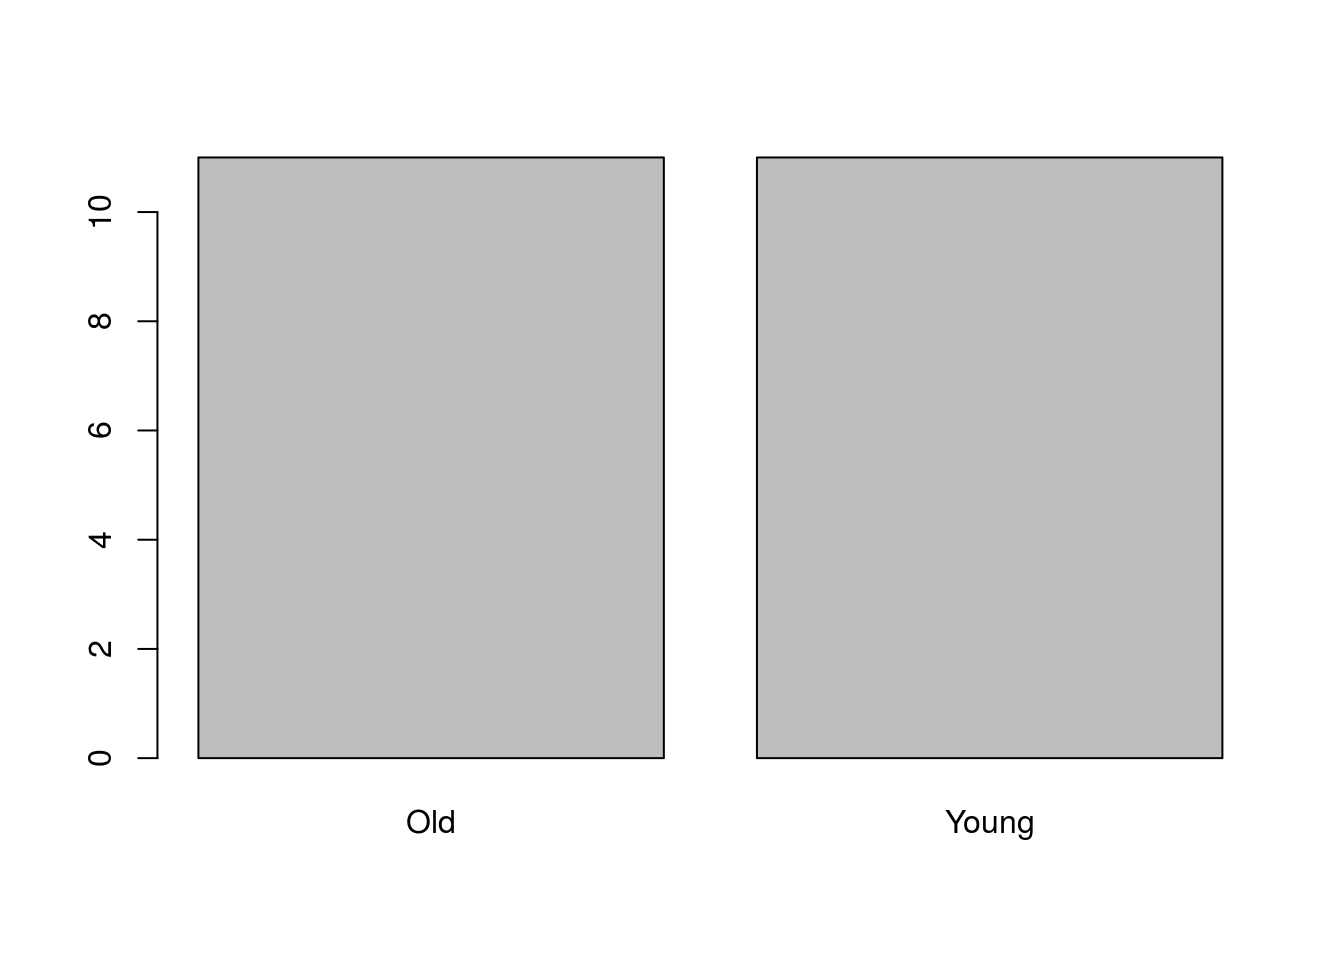
\includegraphics[width=0.5\linewidth]{Rcourse_files/figure-latex/barplot-1}

\subsubsection{Visualizing Bivariate Categorical
Data}\label{visualizing-bivariate-categorical-data}

There are several generalizations of the barplot, aimed to deal with the
visualization of bivariate categorical data. There are sometimes known
as the \emph{clustered bar plot} and the \emph{stacked bar plot}. In
this text, we advocate the use of the \emph{mosaic plot} which is also
the default in R.

\begin{Shaded}
\begin{Highlighting}[]
\KeywordTok{plot}\NormalTok{(table1, }\DataTypeTok{main=}\StringTok{'Bivariate mosaic plot'}\NormalTok{)}
\end{Highlighting}
\end{Shaded}

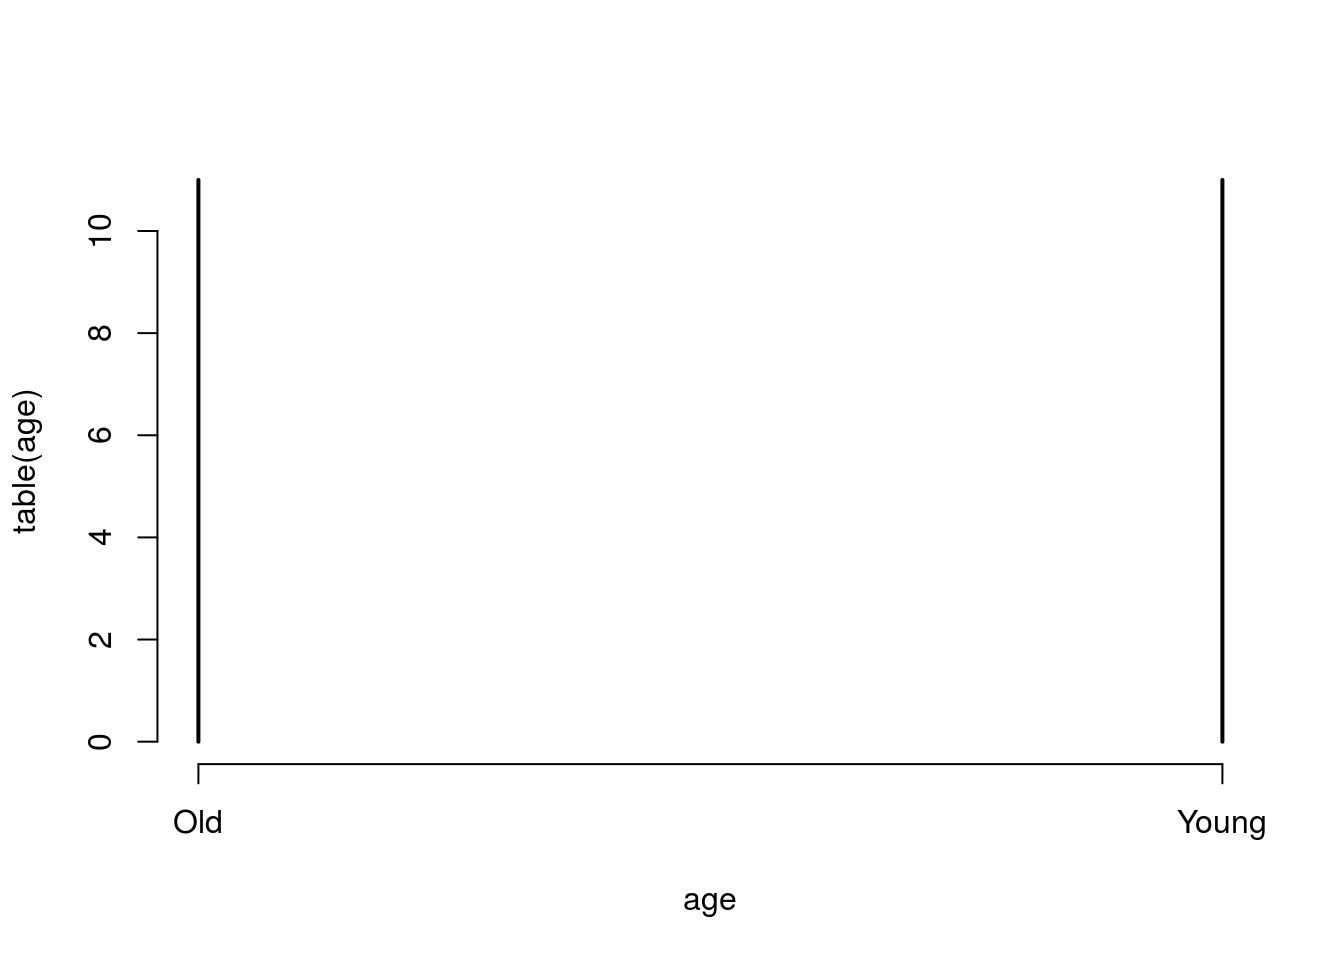
\includegraphics[width=0.5\linewidth]{Rcourse_files/figure-latex/unnamed-chunk-79-1}

\subsubsection{Visualizing Multivariate Categorical
Data}\label{visualizing-multivariate-categorical-data}

The \emph{mosaic plot} is not easy to generalize to more than two
variables, but it is still possible (at the cost of interpretability).

\begin{Shaded}
\begin{Highlighting}[]
\KeywordTok{plot}\NormalTok{(table2}\FloatTok{.1}\NormalTok{, }\DataTypeTok{main=}\StringTok{'Trivaraite mosaic plot'}\NormalTok{)}
\end{Highlighting}
\end{Shaded}

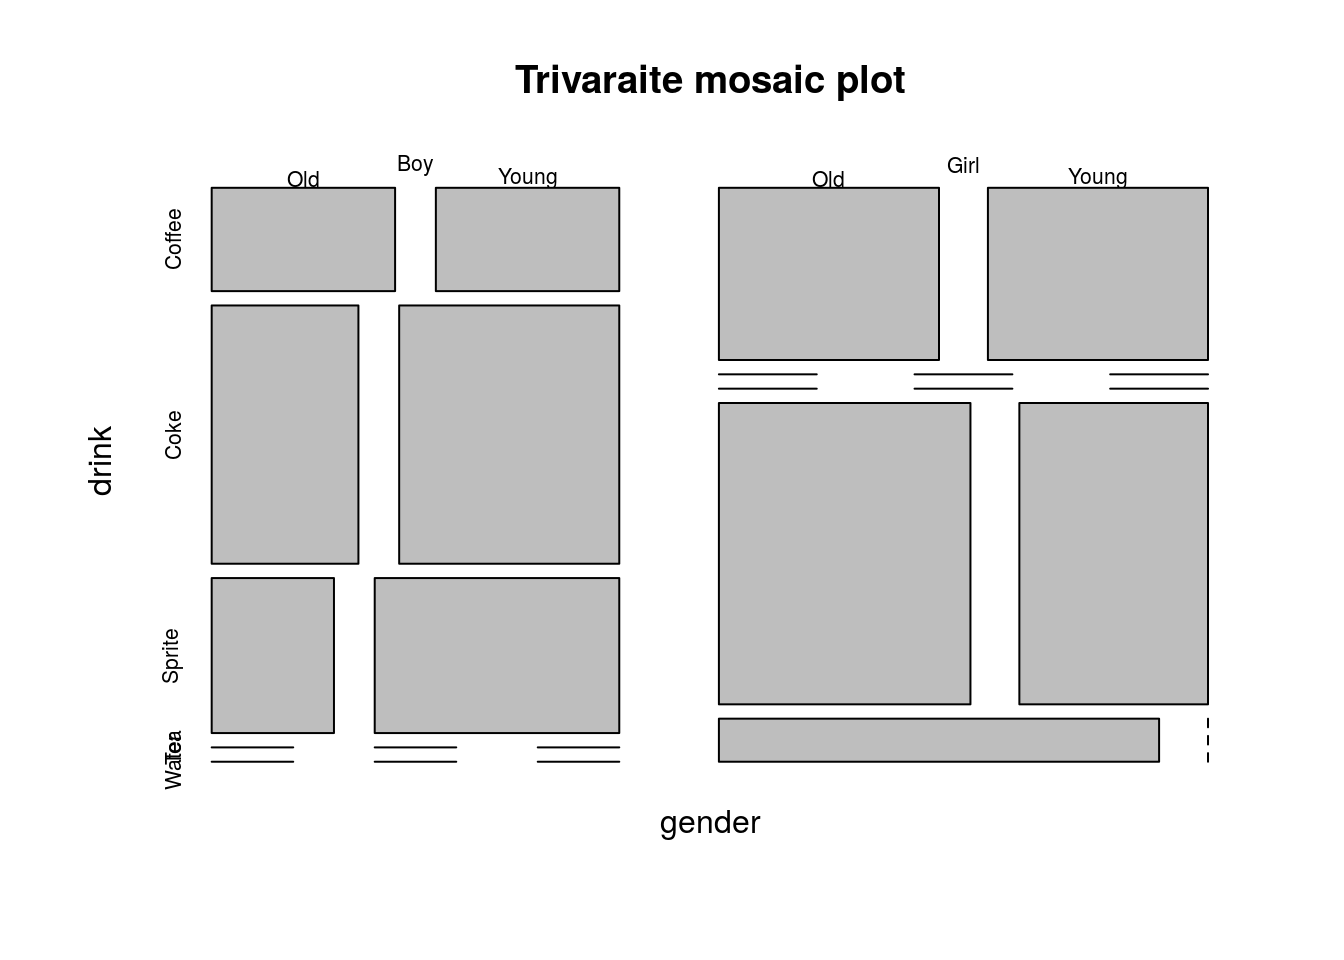
\includegraphics[width=0.5\linewidth]{Rcourse_files/figure-latex/unnamed-chunk-80-1}

\subsection{Continous Data}\label{continous-data-1}

\subsubsection{Visualizing Univariate Continous
Data}\label{visualizing-univariate-continous-data}

There are endlessly many way to visualize continuous univariate data.
The simplest way is to look at the raw data via the \texttt{stripcart}.

\begin{Shaded}
\begin{Highlighting}[]
\NormalTok{sample1 <-}\StringTok{ }\KeywordTok{rexp}\NormalTok{(}\DecValTok{10}\NormalTok{)                             }
\KeywordTok{stripchart}\NormalTok{(sample1)}
\end{Highlighting}
\end{Shaded}

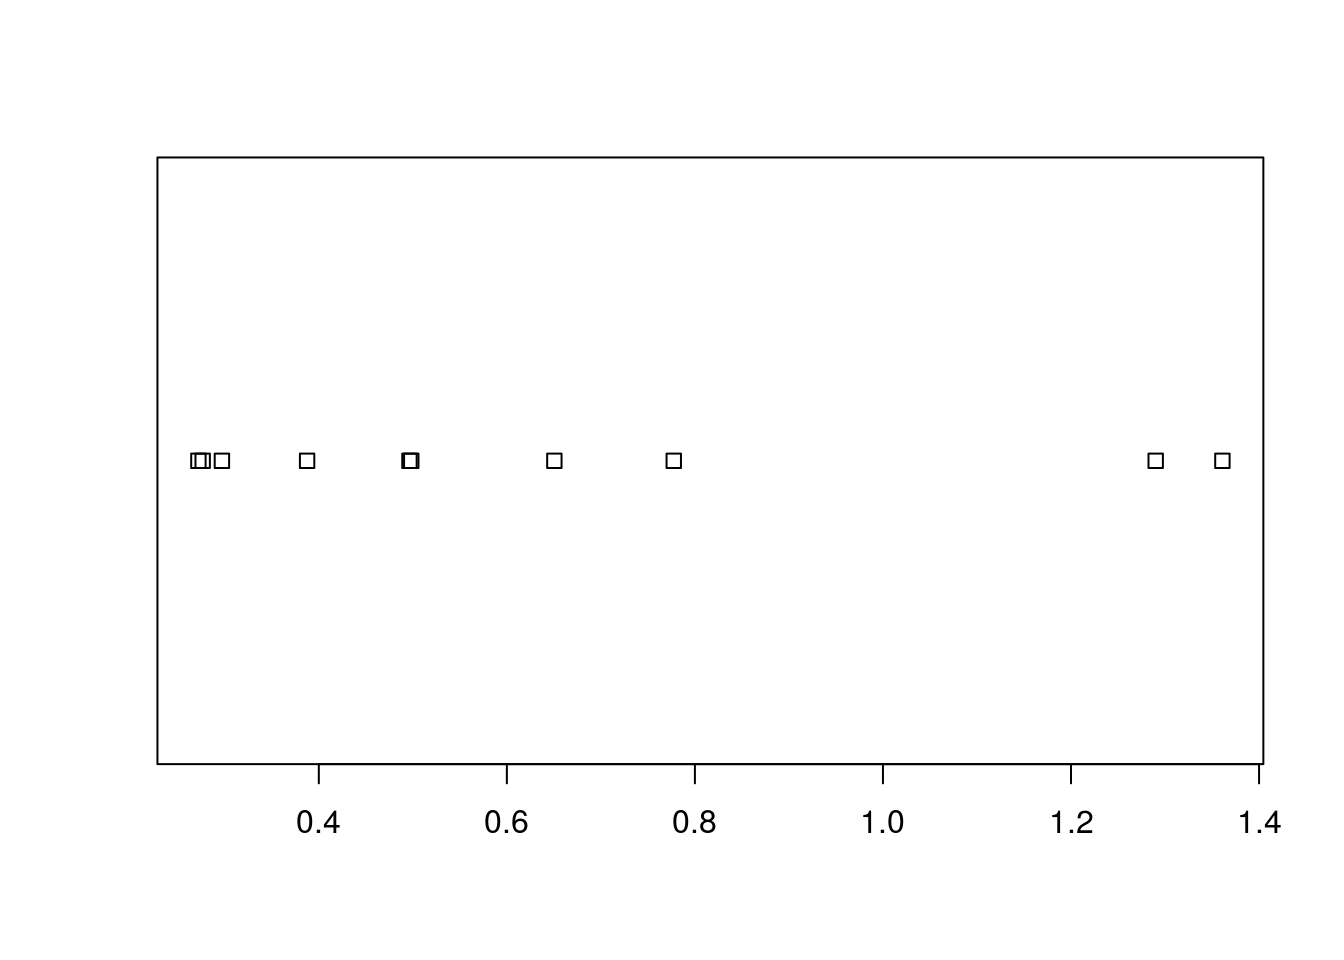
\includegraphics[width=0.5\linewidth]{Rcourse_files/figure-latex/unnamed-chunk-81-1}

Clearly, if there are many observations, the \texttt{stripchart} will be
a useless line of black dots. We thus bin them together, and look at the
frequency of each bin; this is the \emph{histogram}. R's
\texttt{histogram} function has very good defaults to choose the number
of bins.

\begin{Shaded}
\begin{Highlighting}[]
\NormalTok{sample1 <-}\StringTok{ }\KeywordTok{rexp}\NormalTok{(}\DecValTok{100}\NormalTok{)                            }
\KeywordTok{hist}\NormalTok{(sample1, }\DataTypeTok{freq=}\NormalTok{T, }\DataTypeTok{main=}\StringTok{'Counts'}\NormalTok{)        }
\end{Highlighting}
\end{Shaded}

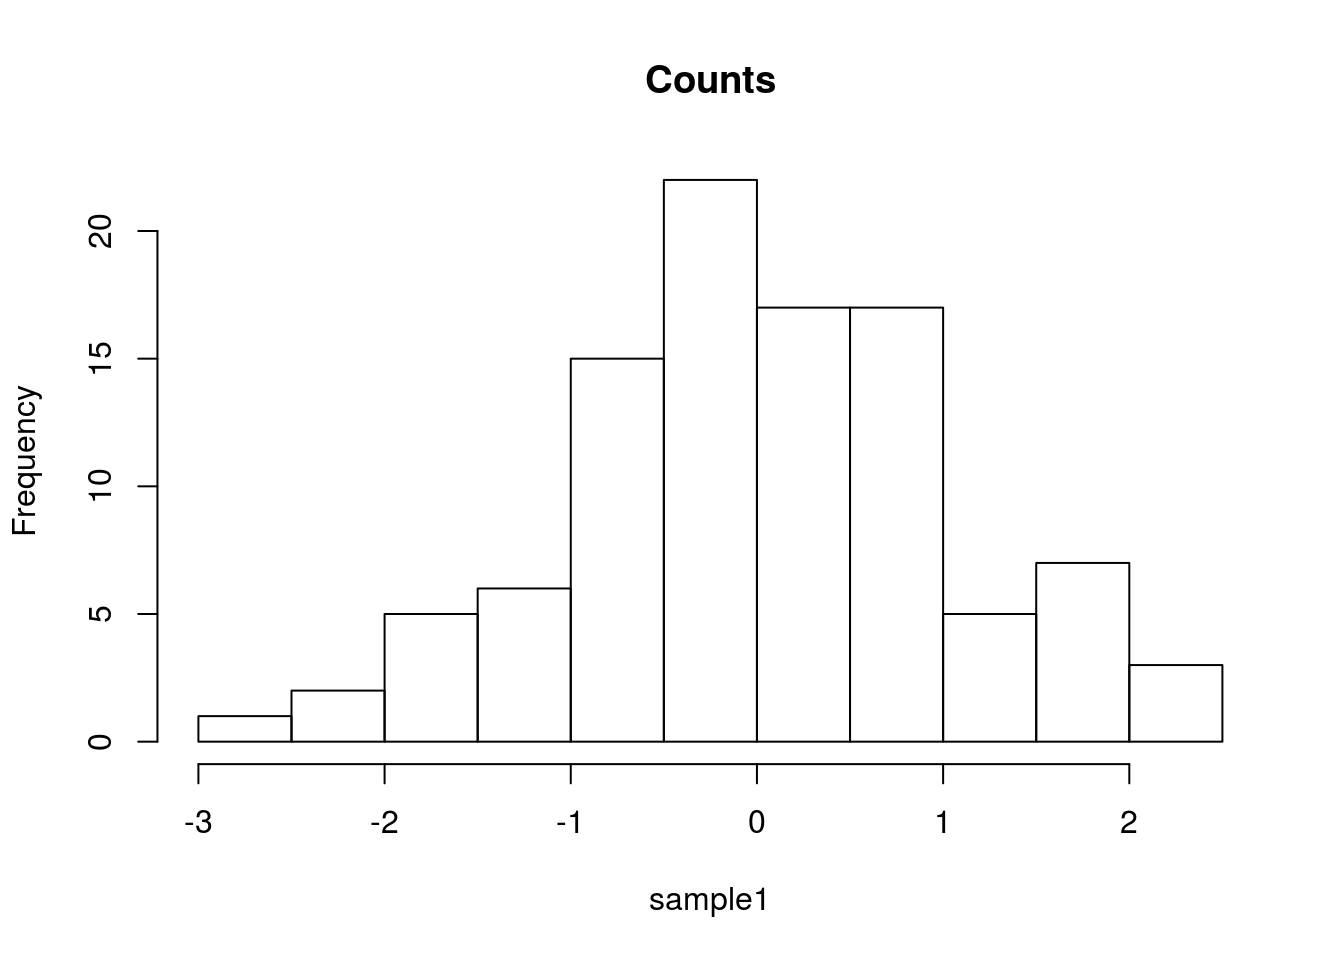
\includegraphics[width=0.5\linewidth]{Rcourse_files/figure-latex/unnamed-chunk-82-1}

\begin{Shaded}
\begin{Highlighting}[]
\KeywordTok{hist}\NormalTok{(sample1, }\DataTypeTok{freq=}\NormalTok{F, }\DataTypeTok{main=}\StringTok{'Frequencies'}\NormalTok{)   }
\end{Highlighting}
\end{Shaded}

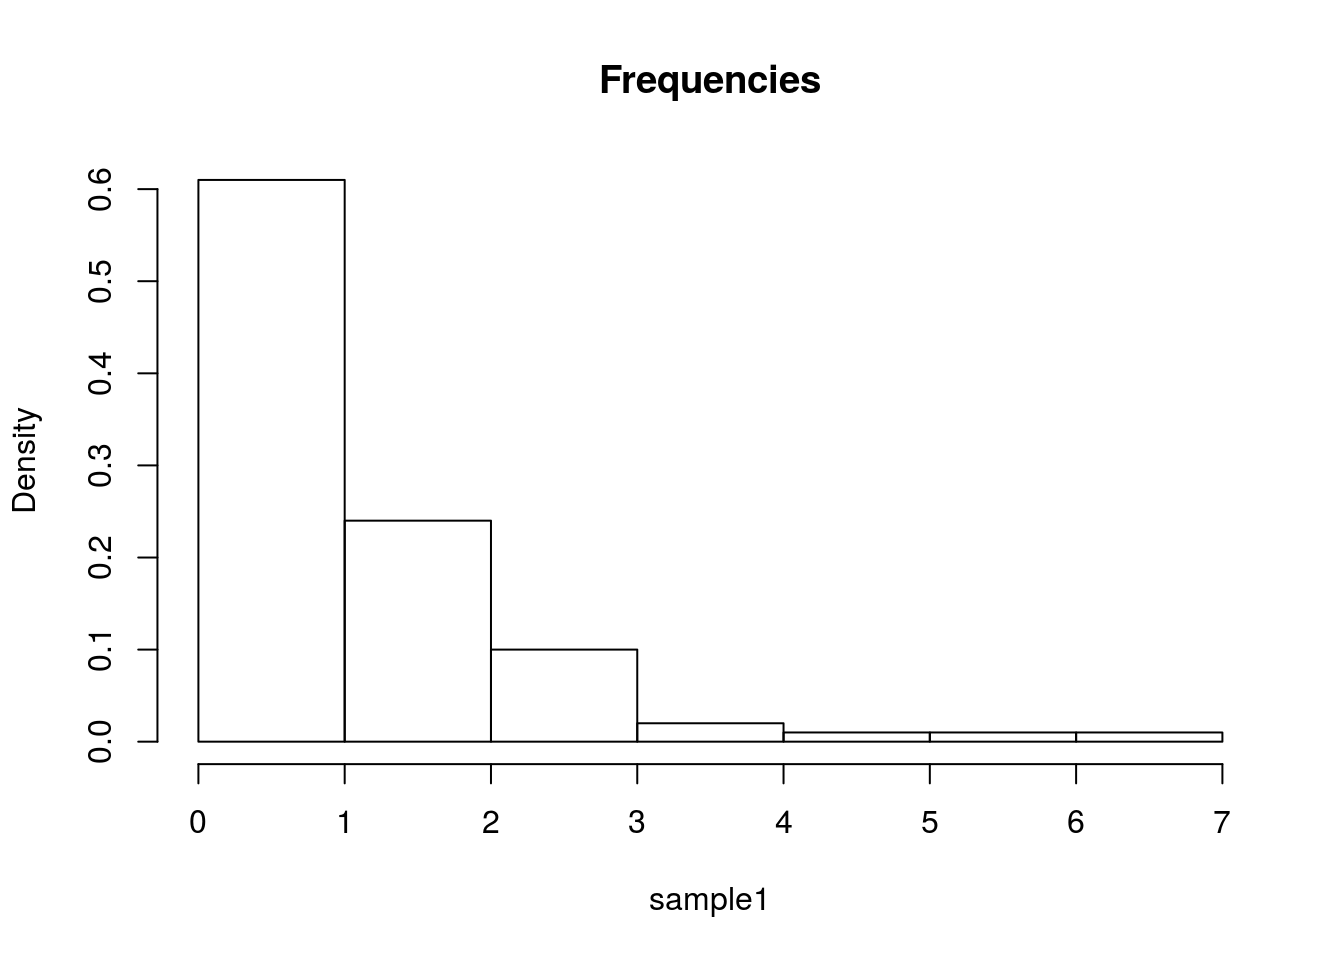
\includegraphics[width=0.5\linewidth]{Rcourse_files/figure-latex/unnamed-chunk-82-2}

The bins of a histogram are non overlapping. We can adopt a sliding
window approach, instead of binning. This is the \emph{density plot}
which is produce with the \texttt{density} functions, and added to an
existing plot with the \texttt{lines} function. The \texttt{rug}
function adds the original data points as ticks on the axes, and is
strongly recommended to detect artifacts due to the binning of the
histogram, or the smoothing of the density plot.

\begin{Shaded}
\begin{Highlighting}[]
\KeywordTok{hist}\NormalTok{(sample1, }\DataTypeTok{freq=}\NormalTok{F, }\DataTypeTok{main=}\StringTok{'Frequencies'}\NormalTok{)   }
\KeywordTok{lines}\NormalTok{(}\KeywordTok{density}\NormalTok{(sample1))                     }
\KeywordTok{rug}\NormalTok{(sample1)}
\end{Highlighting}
\end{Shaded}

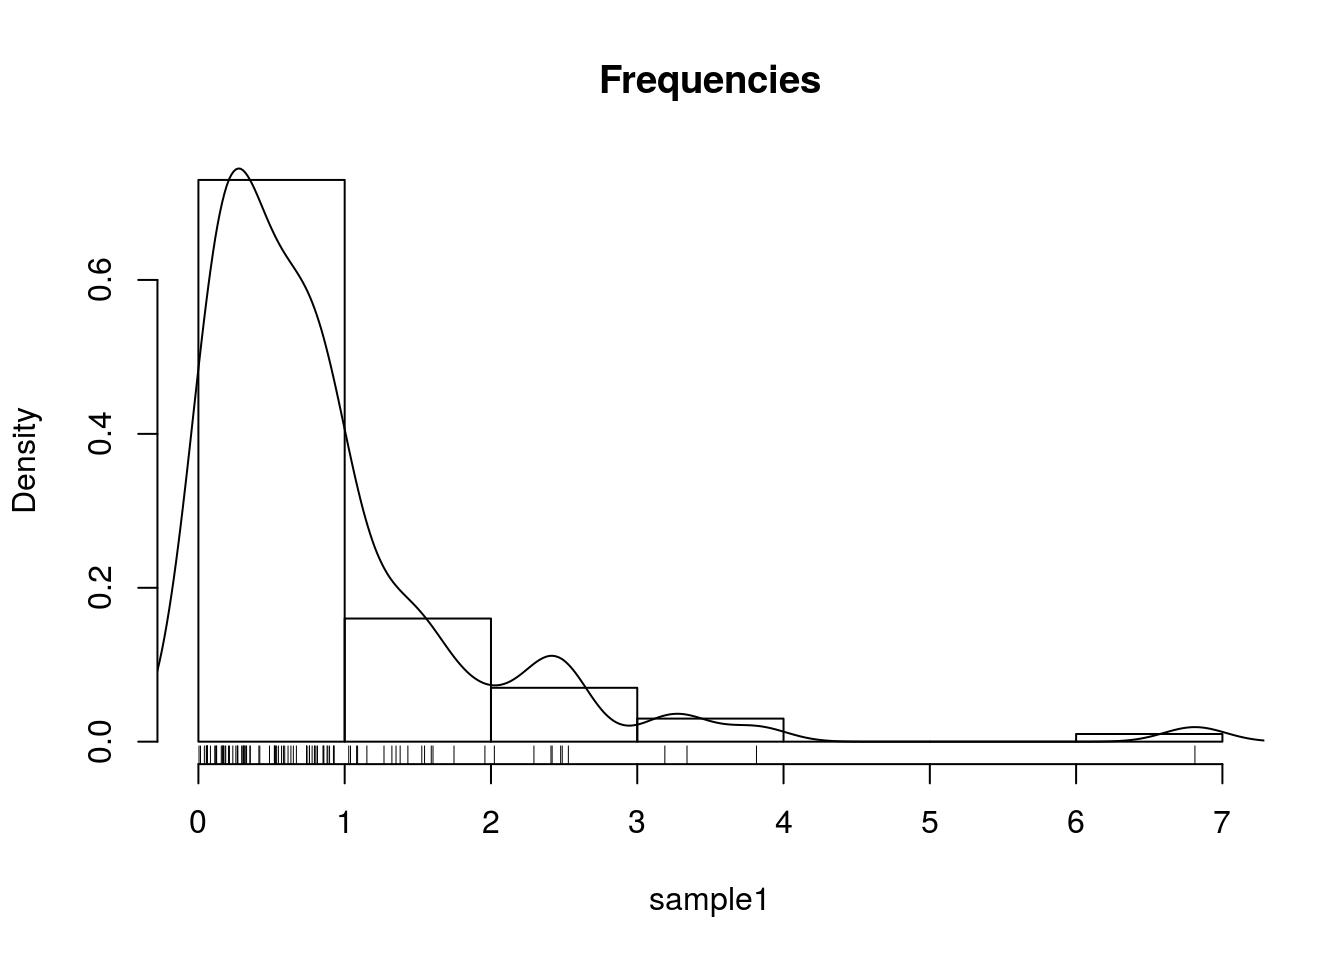
\includegraphics[width=0.5\linewidth]{Rcourse_files/figure-latex/unnamed-chunk-83-1}

\BeginKnitrBlock{remark}
\iffalse {Remark. } \fi Why would it make no sense of making a table, or
a barplot, of continous data?
\EndKnitrBlock{remark}

One particularly useful visualization, due to John w. Tukey, is the
\emph{boxplot}. The boxplot is designed to capture the main phenomena in
the data, and simultaneously point to outlines.

\begin{Shaded}
\begin{Highlighting}[]
\KeywordTok{boxplot}\NormalTok{(sample1)    }
\end{Highlighting}
\end{Shaded}

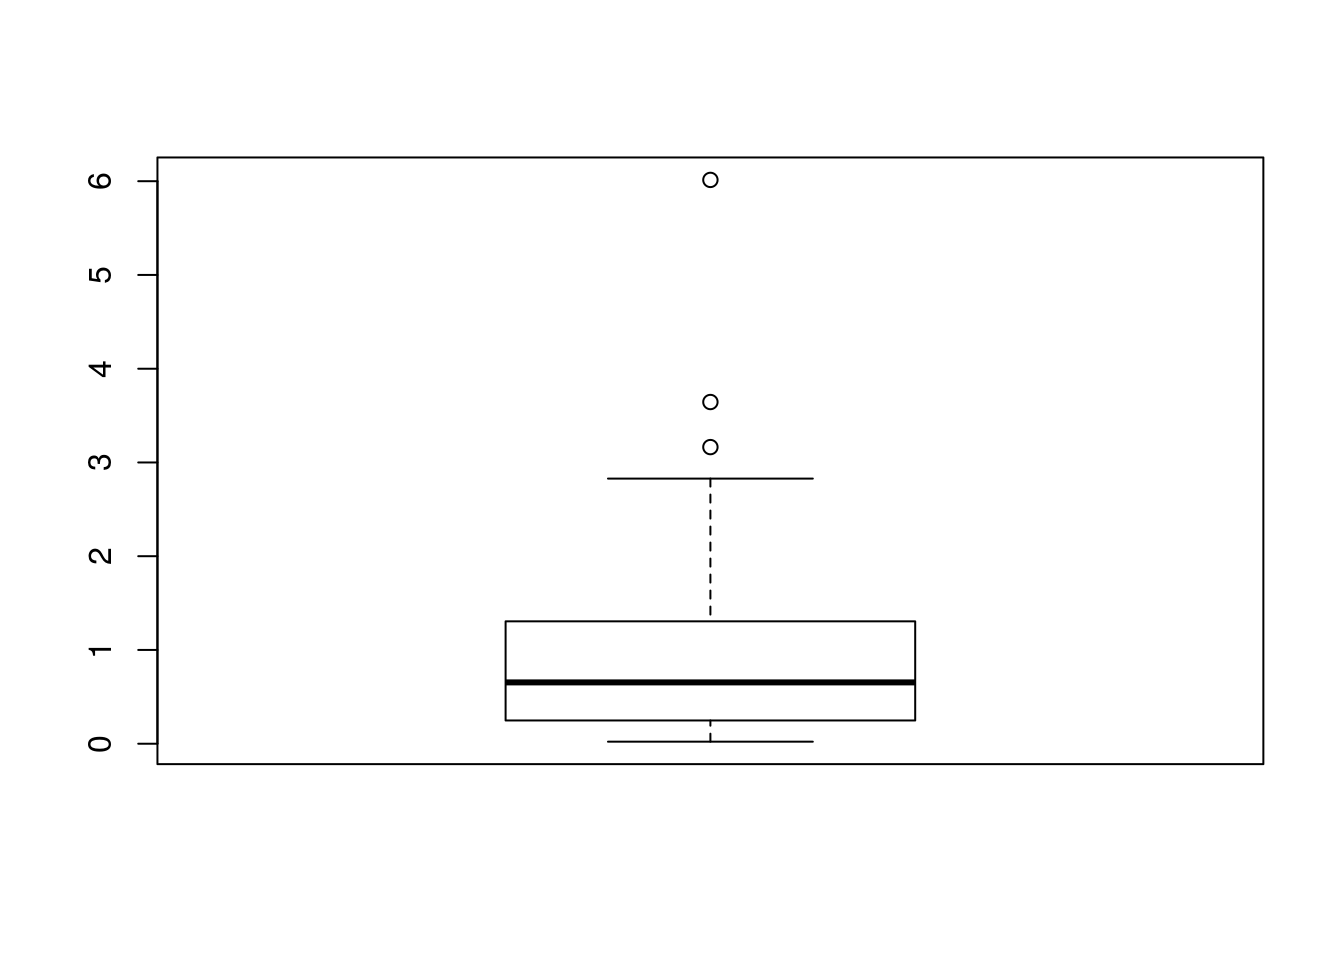
\includegraphics[width=0.5\linewidth]{Rcourse_files/figure-latex/unnamed-chunk-85-1}

\subsubsection{Visualizing Bivariate Continous
Data}\label{visualizing-bivariate-continous-data}

The bivariate counterpart of the \texttt{stipchart} is the celebrated
scatter plot.

\begin{Shaded}
\begin{Highlighting}[]
\NormalTok{n <-}\StringTok{ }\DecValTok{20}
\NormalTok{x1 <-}\StringTok{ }\KeywordTok{rexp}\NormalTok{(n)}
\NormalTok{x2 <-}\StringTok{ }\DecValTok{2}\NormalTok{*}\StringTok{ }\NormalTok{x1 +}\StringTok{ }\DecValTok{4} \NormalTok{+}\StringTok{ }\KeywordTok{rexp}\NormalTok{(n)}
\KeywordTok{plot}\NormalTok{(x2~x1)}
\end{Highlighting}
\end{Shaded}

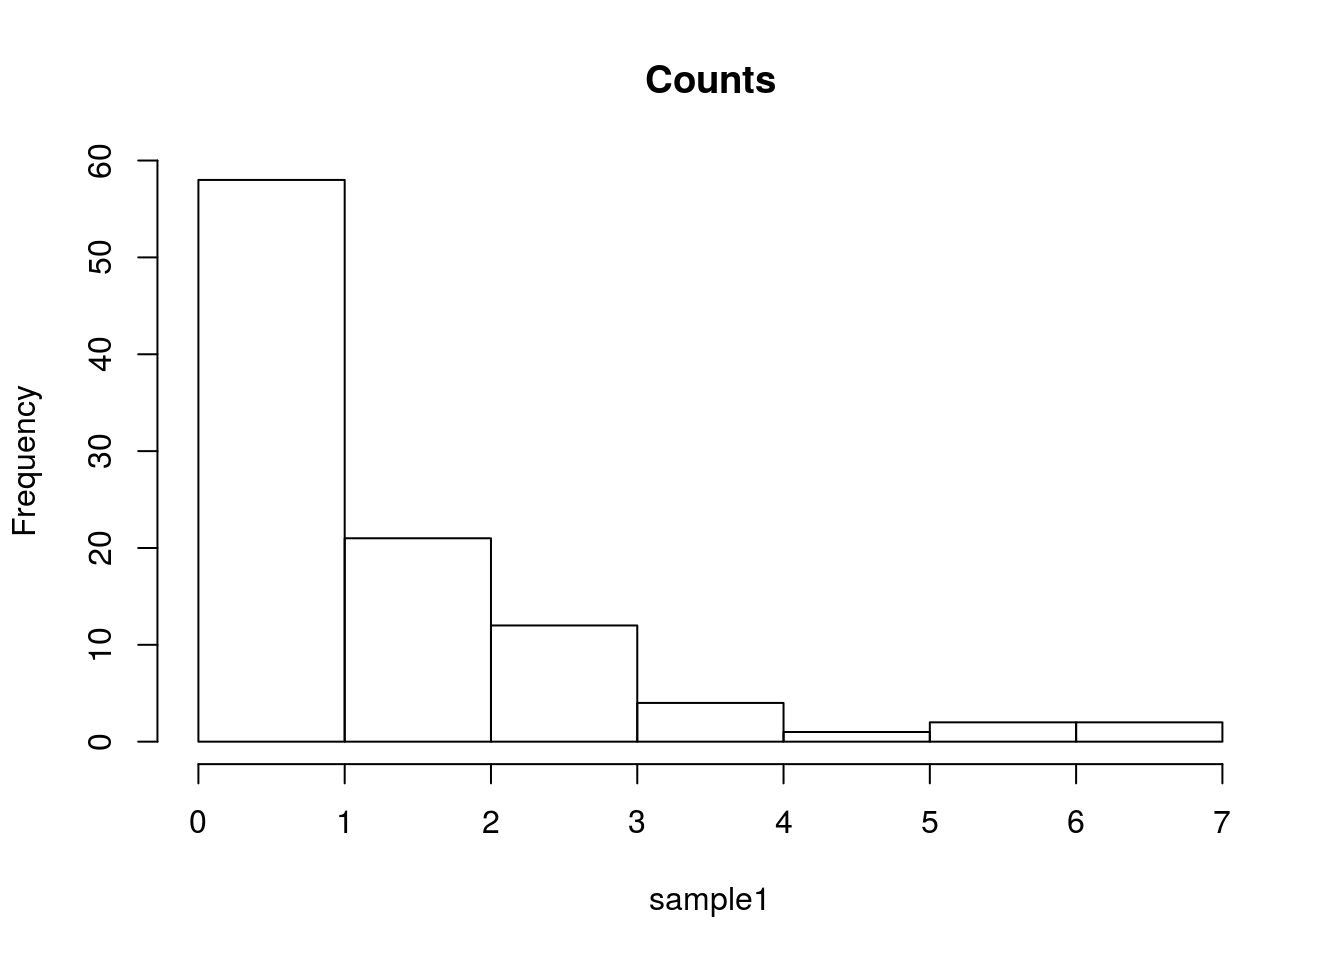
\includegraphics[width=0.5\linewidth]{Rcourse_files/figure-latex/unnamed-chunk-86-1}

Like the univariate \texttt{stripchart}, the scatter plot will be an
uninformative mess in the presence of a lot of data. A nice bivariate
counterpart of the univariate histogram is the \emph{hexbin plot}, which
tessellates the bivariate plane with hexagons.

\begin{Shaded}
\begin{Highlighting}[]
\KeywordTok{library}\NormalTok{(hexbin)}
\NormalTok{n <-}\StringTok{ }\FloatTok{2e5}
\NormalTok{x1 <-}\StringTok{ }\KeywordTok{rexp}\NormalTok{(n)}
\NormalTok{x2 <-}\StringTok{ }\DecValTok{2}\NormalTok{*}\StringTok{ }\NormalTok{x1 +}\StringTok{ }\DecValTok{4} \NormalTok{+}\StringTok{ }\KeywordTok{rnorm}\NormalTok{(n)}
\KeywordTok{plot}\NormalTok{(}\KeywordTok{hexbin}\NormalTok{(}\DataTypeTok{x =} \NormalTok{x1, }\DataTypeTok{y =} \NormalTok{x2))}
\end{Highlighting}
\end{Shaded}

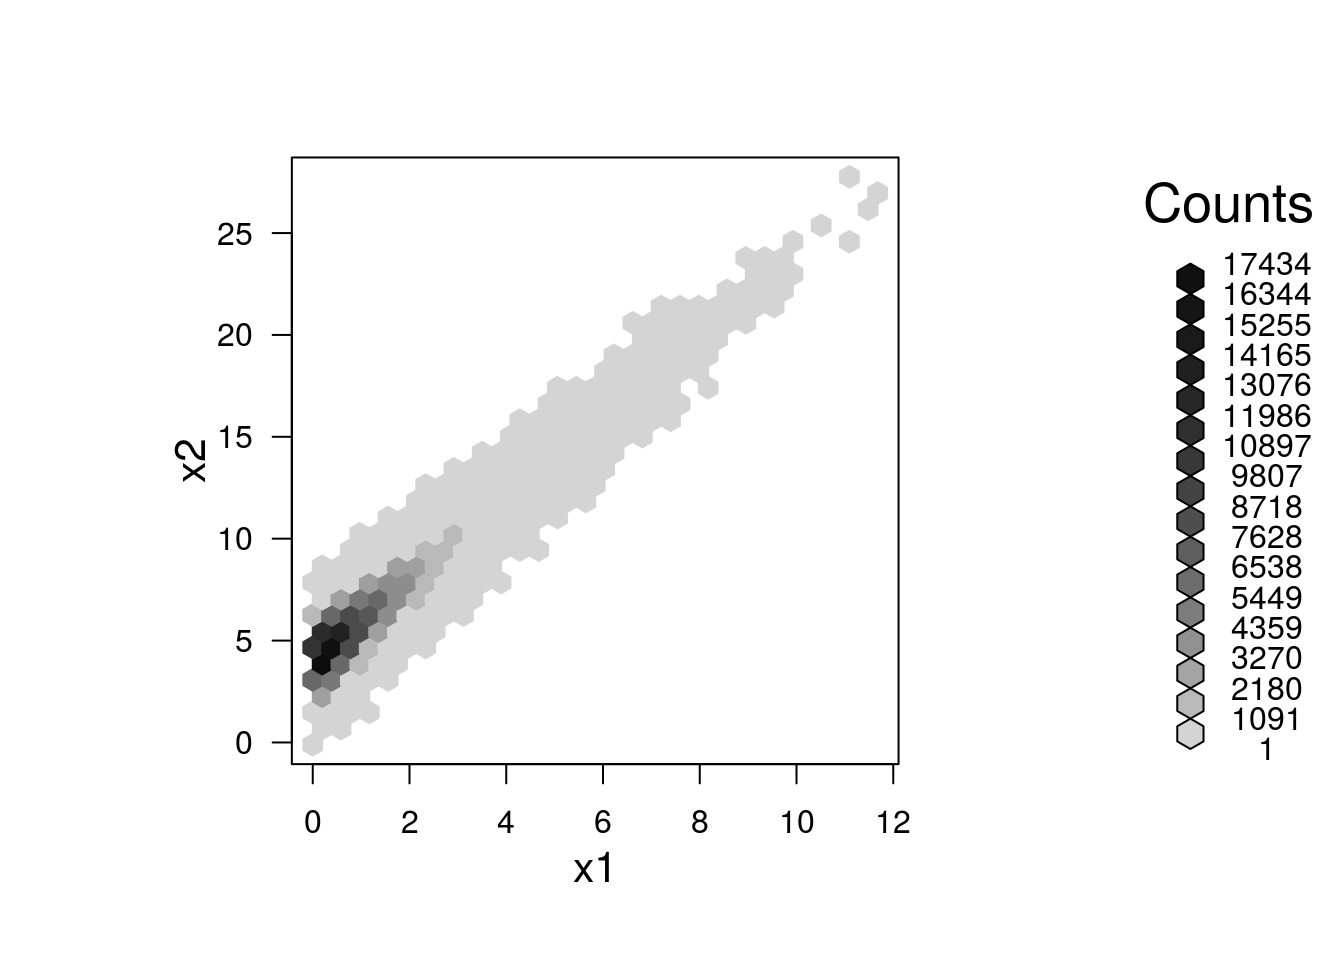
\includegraphics[width=0.5\linewidth]{Rcourse_files/figure-latex/unnamed-chunk-87-1}

\subsubsection{Visualizing Multivariate Continous
Data}\label{visualizing-multivariate-continous-data}

Visualizing multivariate data is a tremendous challenge given that we
cannot grasp \(4\) dimensional spaces, nor can the computer screen
present more than \(2\) dimensional spaces. We thus have several
options: (i) To project the data to 2D. This is discussed in the
Dimensionality Reduction section (\ref{dim-reduce}). (ii) To visualize
not the data, but the summaries. Like the covariance matrix.

Since the covariance matrix, \(\hat \Sigma\) is a matrix, it can be
visualized as a matrix.

\begin{Shaded}
\begin{Highlighting}[]
\NormalTok{covariance <-}\StringTok{ }\KeywordTok{cov}\NormalTok{(longley) }\CommentTok{# The covariance of the longley dataset}
\NormalTok{lattice::}\KeywordTok{levelplot}\NormalTok{(covariance)}
\end{Highlighting}
\end{Shaded}

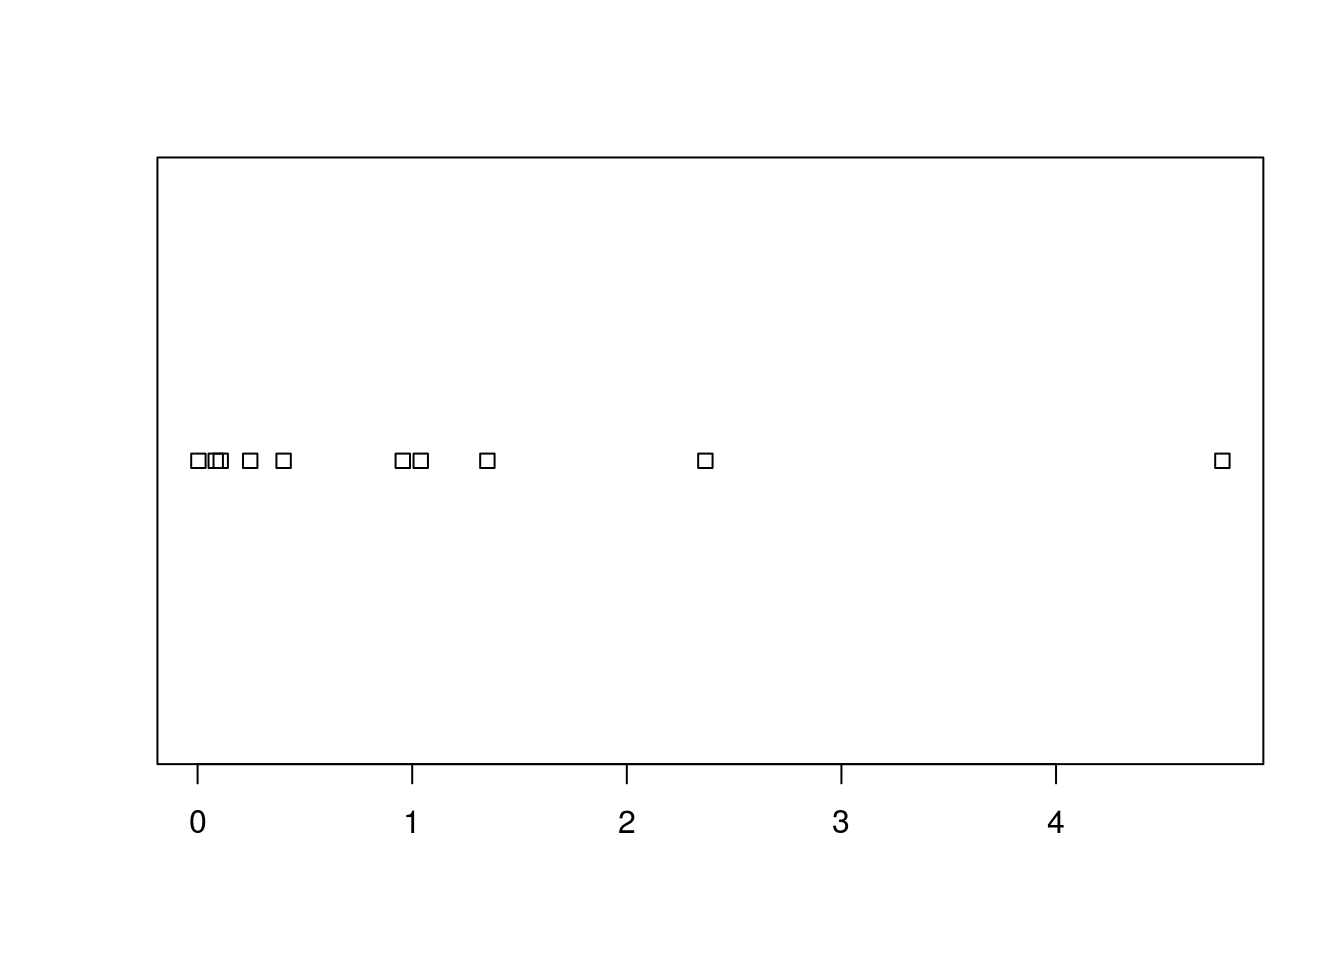
\includegraphics[width=0.5\linewidth]{Rcourse_files/figure-latex/unnamed-chunk-88-1}

\section{Bibliographic Notes}\label{bibliographic-notes-2}

Like any other topic in this book, you can consult
\citet{venables2013modern}. The seminal book on EDA, written long before
R was around, is \citet{tukey1977exploratory}.

\chapter{Linear Models}\label{lm}

\section{Problem Setup}\label{problem-setup}

\BeginKnitrBlock{example}
\protect\hypertarget{ex:cap-experiment}{}{\label{ex:cap-experiment}}Consider
a randomized experiment designed to study the effects of temperature and
pressure on the diameter of a bottle cap.
\EndKnitrBlock{example}

\BeginKnitrBlock{example}
\protect\hypertarget{ex:rental}{}{\label{ex:rental}}Consider the prediction
of rental prices given an appartment's attributes.
\EndKnitrBlock{example}

Both examples require some statistical model, but they are very
different. The first is a \emph{causal inference} problem: we want to
design an intervention so that we need to recover the causal effect of
temperature and pressure. The second is a \emph{prediction} problem. We
don't care about the causal effects, we just want good predictions.

In this chapter we discuss the causal problem in Example
\ref{ex:cap-experiment}. This means that when we assume a model, we
assume it is the actual \emph{data generating process}. The second type
of problems is discussed in the Supervised Learning Chapter
\ref{supervised}.

Lets present the linear model. We assume that a response\footnote{The
  ``response'' is also know as the ``dependent'' variable, of the
  ``labels'' in the machine learning literature.} variable is the sum of
effects of some factors\footnote{The ``factors'' are also known as the
  ``independent variable'', the ``design'', the ``features'' and the
  ``attributes''.}. Denoting the dependent by \(y\), the factors by
\(x\), and the effects by \(\beta\) the linear model assumption implies
that

\begin{align}
  E[y]=\sum_j x_j \beta_j=x'\beta .
  \label{eq:linear-mean}
\end{align}

Clearly, there may be other factors that affect the the caps' diameters.
We thus introduce an error term\footnote{The ``error term'' is also
  known as the ``noise'', or the ``common causes of variability''.},
denoted by \(\varepsilon\), to capture the effects of all unmodeled
factors. The implied generative process of a sample of \(i=1,\dots,n\)
observations it thus

\begin{align}
  y_i = \sum x_{i,j} \beta_j + \varepsilon_i , i=1,\dots,n .
  \label{eq:linear-observed}
\end{align}

or in matrix notation

\begin{align}
  y = X \beta + \varepsilon .
  \label{eq:linear-matrix}
\end{align}

Lets demonstrate Eq.\eqref{eq:linear-observed}:

In our cap example, assuming that pressure and temperature have two
levels each (say, high and low), we would write \(x_{i,1}=1\) if the
pressure of the \(i\)'th measurement was set to high, and \(x_{i,1}=-1\)
if the pressure was set to low. Similarly, we would write \(x_{i,2}=1\),
and \(x_{i,2}=-1\), if the temperature was set to high, or low,
respectively. The coding with \(\{-1,1\}\) is known as \emph{effect
coding}. If you prefer coding with \(\{0,1\}\), this is known as
\emph{dummy coding}.

In Gosset's classical regression problem, where we try to seek the
relation between the heights of sons and fathers then \(p=1\), \(y_i\)
is the height of the \(i\)'th father, and \(x_i\) the height of the
\(i\)'th son.

There are many reasons these models are so popular:

\begin{enumerate}
\def\labelenumi{\arabic{enumi}.}
\item
  Before the computer age, these were pretty much the only models that
  could actually be computed\footnote{By ``computed'' we mean what
    statisticians call ``fitted'', or ``estimated'', and computer
    scientists call ``learned''.}. The whole Analysis of Variance
  (ANOVA) literature is an instance of linear models.
\item
  For purposes of prediction, where the actual data generating process
  is not of primary importance, they are popular because they simply
  work. Why is that? They are simple so that they do not require a lot
  of data to be computed. Put differently, they may be biased, but their
  variance is small enough to make them more accurate than other models.
\item
  For categorical or factorial predictors, \textbf{any} functional
  relation can be cast as a linear model.
\item
  For the purpose of \emph{screening}, where we only want to show the
  existence of an effect, and are less interested in the magnitude of
  the effect, a linear model is enough.
\item
  If the true generative relation is not linear, but smooth enough, then
  the linear function is a good approximation via Taylor's theorem.
\end{enumerate}

There are still two matters we have to attend: How the estimate
\(\beta\), and how to perform inference.

In linear models the estimation of \(\beta\) is done using the method of
least squares. For this reason, a linear model with least squares
estimation is known as Ordinary Least Squares (OLS). The OLS problem:

\begin{align}
  \hat \beta_{OLS}:= argmin_\beta \{ \sum_i (y_i-x_i'\beta)^2 \},
  \label{eq:ols}
\end{align}

and in matrix notation

\begin{align}
  \hat \beta_{OLS}:= argmin_\beta \{ \Vert y-X\beta \Vert^2_2 \}.
  \label{eq:ols-matrix}
\end{align}

\BeginKnitrBlock{remark}
\iffalse {Remark. } \fi Personally, I prefer the matrix notation because
it suggests of the geometry of the problem. The reader is referred to
\citet{friedman2001elements}, Sec 3.2, for more on the geometry of OLS.
\EndKnitrBlock{remark}

Different software suits, and even different R packages, solve
Eq.\eqref{eq:ols} in different ways so that we skip the details of how
exactly it is solved.

The last matter we need to attend is how to do inference on
\(\hat \beta_{OLS}\). For that, we will need some assumptions on
\(\varepsilon\). A typical set of assumptions is the following:

\begin{enumerate}
\def\labelenumi{\arabic{enumi}.}
\tightlist
\item
  \textbf{Independence}: we assume \(\varepsilon_i\) are independent of
  everything else. Think of them as the measurement error of an
  instrument: it is independent of the measured value and of previous
  measurements.
\item
  \textbf{Centered}: we assume that \(E[\varepsilon]=0\), meaning there
  is no systematic error.
\item
  \textbf{Normality}: we will typically assume that
  \(\varepsilon \sim \mathcal{N}(0,\sigma^2)\), but we will later see
  that this is not really required.
\end{enumerate}

We emphasize that these assumptions are only needed for inference on
\(\hat \beta\) and not for the estimation itself, which is done by the
purely algorithmic framework of OLS.

Given the above assumptions, we can apply some probability theory and
linear algebra to get

\begin{align}
  \hat \beta_{OLS} \sim \mathcal{N}(\beta, (X'X)^{-1} \sigma^2)
  \label{eq:ols-distribution}
\end{align}

The reason I am not too strict about the normality assumption above, is
that Eq.\eqref{eq:ols-distribution} is approximately correct even if
\(\varepsilon\) is not normal, provided that there are many more
observations than factors (\(n \gg p\)).

\section{OLS Estimation}\label{ols-estimation}

We are now ready to estimate some linear models with R. We will use the
\texttt{whiteside} data from the \textbf{MASS} package,recording the
outside temperature and gas consumption, before and after insulation.

\begin{Shaded}
\begin{Highlighting}[]
\KeywordTok{library}\NormalTok{(MASS)}
\KeywordTok{data}\NormalTok{(whiteside)}
\KeywordTok{head}\NormalTok{(whiteside) }\CommentTok{# inspect the data}
\end{Highlighting}
\end{Shaded}

\begin{verbatim}
##    Insul Temp Gas
## 1 Before -0.8 7.2
## 2 Before -0.7 6.9
## 3 Before  0.4 6.4
## 4 Before  2.5 6.0
## 5 Before  2.9 5.8
## 6 Before  3.2 5.8
\end{verbatim}

We do the OLS estimation with \texttt{lm} function, possibly the most
important function in R.

\begin{Shaded}
\begin{Highlighting}[]
\NormalTok{lm}\FloatTok{.1} \NormalTok{<-}\StringTok{ }\KeywordTok{lm}\NormalTok{(Gas~Temp, }\DataTypeTok{data=}\NormalTok{whiteside[whiteside$Insul==}\StringTok{'Before'}\NormalTok{,]) }\CommentTok{# OLS estimation }
\end{Highlighting}
\end{Shaded}

Things to note:

\begin{itemize}
\tightlist
\item
  We used the tilde syntax \texttt{Gas\textasciitilde{}Temp}, reading
  ``gas as linear function of temperature''.
\item
  The \texttt{data} argument tells R where to look for the variables Gas
  and Temp. We used only observations before the insulation.
\item
  The result is assigned to the object \texttt{lm.1}.
\end{itemize}

Alternative formulations with the same results would be

\begin{Shaded}
\begin{Highlighting}[]
\NormalTok{lm}\FloatTok{.1} \NormalTok{<-}\StringTok{ }\KeywordTok{lm}\NormalTok{(}\DataTypeTok{y=}\NormalTok{Gas, }\DataTypeTok{x=}\NormalTok{Temp, }\DataTypeTok{data=}\NormalTok{whiteside[whiteside$Insul==}\StringTok{'Before'}\NormalTok{,]) }
\NormalTok{lm}\FloatTok{.1} \NormalTok{<-}\StringTok{ }\KeywordTok{lm}\NormalTok{(}\DataTypeTok{y=}\NormalTok{whiteside[whiteside$Insul==}\StringTok{'Before'}\NormalTok{,]$Gas, }\DataTypeTok{x=}\NormalTok{whiteside[whiteside$Insul==}\StringTok{'Before'}\NormalTok{,]$Temp)  }
\end{Highlighting}
\end{Shaded}

The output is an object of class \texttt{lm}.

\begin{Shaded}
\begin{Highlighting}[]
\KeywordTok{class}\NormalTok{(lm}\FloatTok{.1}\NormalTok{)}
\end{Highlighting}
\end{Shaded}

\begin{verbatim}
## [1] "lm"
\end{verbatim}

Objects of class \texttt{lm} are very complicated. It stored a lot of
information which will be later used for inference, plotting, etc. The
\texttt{str} function, short for ``structure'' shows us the various
elements of the object.

\begin{Shaded}
\begin{Highlighting}[]
\KeywordTok{str}\NormalTok{(lm}\FloatTok{.1}\NormalTok{)}
\end{Highlighting}
\end{Shaded}

\begin{verbatim}
## List of 12
##  $ coefficients : Named num [1:2] 6.854 -0.393
##   ..- attr(*, "names")= chr [1:2] "(Intercept)" "Temp"
##  $ residuals    : Named num [1:26] 0.0316 -0.2291 -0.2965 0.1293 0.0866 ...
##   ..- attr(*, "names")= chr [1:26] "1" "2" "3" "4" ...
##  $ effects      : Named num [1:26] -24.2203 -5.6485 -0.2541 0.1463 0.0988 ...
##   ..- attr(*, "names")= chr [1:26] "(Intercept)" "Temp" "" "" ...
##  $ rank         : int 2
##  $ fitted.values: Named num [1:26] 7.17 7.13 6.7 5.87 5.71 ...
##   ..- attr(*, "names")= chr [1:26] "1" "2" "3" "4" ...
##  $ assign       : int [1:2] 0 1
##  $ qr           :List of 5
##   ..$ qr   : num [1:26, 1:2] -5.099 0.196 0.196 0.196 0.196 ...
##   .. ..- attr(*, "dimnames")=List of 2
##   .. .. ..$ : chr [1:26] "1" "2" "3" "4" ...
##   .. .. ..$ : chr [1:2] "(Intercept)" "Temp"
##   .. ..- attr(*, "assign")= int [1:2] 0 1
##   ..$ qraux: num [1:2] 1.2 1.35
##   ..$ pivot: int [1:2] 1 2
##   ..$ tol  : num 1e-07
##   ..$ rank : int 2
##   ..- attr(*, "class")= chr "qr"
##  $ df.residual  : int 24
##  $ xlevels      : Named list()
##  $ call         : language lm(formula = Gas ~ Temp, data = whiteside[whiteside$Insul == "Before",      ])
##  $ terms        :Classes 'terms', 'formula'  language Gas ~ Temp
##   .. ..- attr(*, "variables")= language list(Gas, Temp)
##   .. ..- attr(*, "factors")= int [1:2, 1] 0 1
##   .. .. ..- attr(*, "dimnames")=List of 2
##   .. .. .. ..$ : chr [1:2] "Gas" "Temp"
##   .. .. .. ..$ : chr "Temp"
##   .. ..- attr(*, "term.labels")= chr "Temp"
##   .. ..- attr(*, "order")= int 1
##   .. ..- attr(*, "intercept")= int 1
##   .. ..- attr(*, "response")= int 1
##   .. ..- attr(*, ".Environment")=<environment: R_GlobalEnv> 
##   .. ..- attr(*, "predvars")= language list(Gas, Temp)
##   .. ..- attr(*, "dataClasses")= Named chr [1:2] "numeric" "numeric"
##   .. .. ..- attr(*, "names")= chr [1:2] "Gas" "Temp"
##  $ model        :'data.frame':   26 obs. of  2 variables:
##   ..$ Gas : num [1:26] 7.2 6.9 6.4 6 5.8 5.8 5.6 4.7 5.8 5.2 ...
##   ..$ Temp: num [1:26] -0.8 -0.7 0.4 2.5 2.9 3.2 3.6 3.9 4.2 4.3 ...
##   ..- attr(*, "terms")=Classes 'terms', 'formula'  language Gas ~ Temp
##   .. .. ..- attr(*, "variables")= language list(Gas, Temp)
##   .. .. ..- attr(*, "factors")= int [1:2, 1] 0 1
##   .. .. .. ..- attr(*, "dimnames")=List of 2
##   .. .. .. .. ..$ : chr [1:2] "Gas" "Temp"
##   .. .. .. .. ..$ : chr "Temp"
##   .. .. ..- attr(*, "term.labels")= chr "Temp"
##   .. .. ..- attr(*, "order")= int 1
##   .. .. ..- attr(*, "intercept")= int 1
##   .. .. ..- attr(*, "response")= int 1
##   .. .. ..- attr(*, ".Environment")=<environment: R_GlobalEnv> 
##   .. .. ..- attr(*, "predvars")= language list(Gas, Temp)
##   .. .. ..- attr(*, "dataClasses")= Named chr [1:2] "numeric" "numeric"
##   .. .. .. ..- attr(*, "names")= chr [1:2] "Gas" "Temp"
##  - attr(*, "class")= chr "lm"
\end{verbatim}

At this point, we only want \(\hat \beta_{OLS}\) which can be extracted
with the \texttt{coef} function.

\begin{Shaded}
\begin{Highlighting}[]
\KeywordTok{coef}\NormalTok{(lm}\FloatTok{.1}\NormalTok{)}
\end{Highlighting}
\end{Shaded}

\begin{verbatim}
## (Intercept)        Temp 
##   6.8538277  -0.3932388
\end{verbatim}

Things to note:

\begin{itemize}
\item
  R automatically adds an \texttt{(Intercept)} term. This means we
  estimate \(y_i=\beta_0 + \beta_1 Gas + \varepsilon\) and not
  \(y_i=\beta_1 Gas + \varepsilon_i\). This makes sense because we are
  interested in the variability of the gas consumption about its mean,
  and not about zero.
\item
  The effect of temperature, i.e., \(\hat \beta_1\), is -0.39. The
  negative sign means that the higher the temperature, the less gas is
  consumed. The magnitude of the coefficient means that for a unit
  increase in the outside temperature, the gas consumption decreases by
  0.39 units.
\end{itemize}

We can use the \texttt{predict} function to make predictions, but we
emphasize that if the purpose of the model is to make predictions, and
not interpret coefficients, better skip to The Supervised Learning
Chapter \ref{supervised}.

\begin{Shaded}
\begin{Highlighting}[]
\KeywordTok{plot}\NormalTok{(}\KeywordTok{predict}\NormalTok{(lm}\FloatTok{.1}\NormalTok{)~whiteside[whiteside$Insul==}\StringTok{'Before'}\NormalTok{,]$Gas)}
\KeywordTok{abline}\NormalTok{(}\DecValTok{0}\NormalTok{,}\DecValTok{1}\NormalTok{, }\DataTypeTok{lty=}\DecValTok{2}\NormalTok{)}
\end{Highlighting}
\end{Shaded}

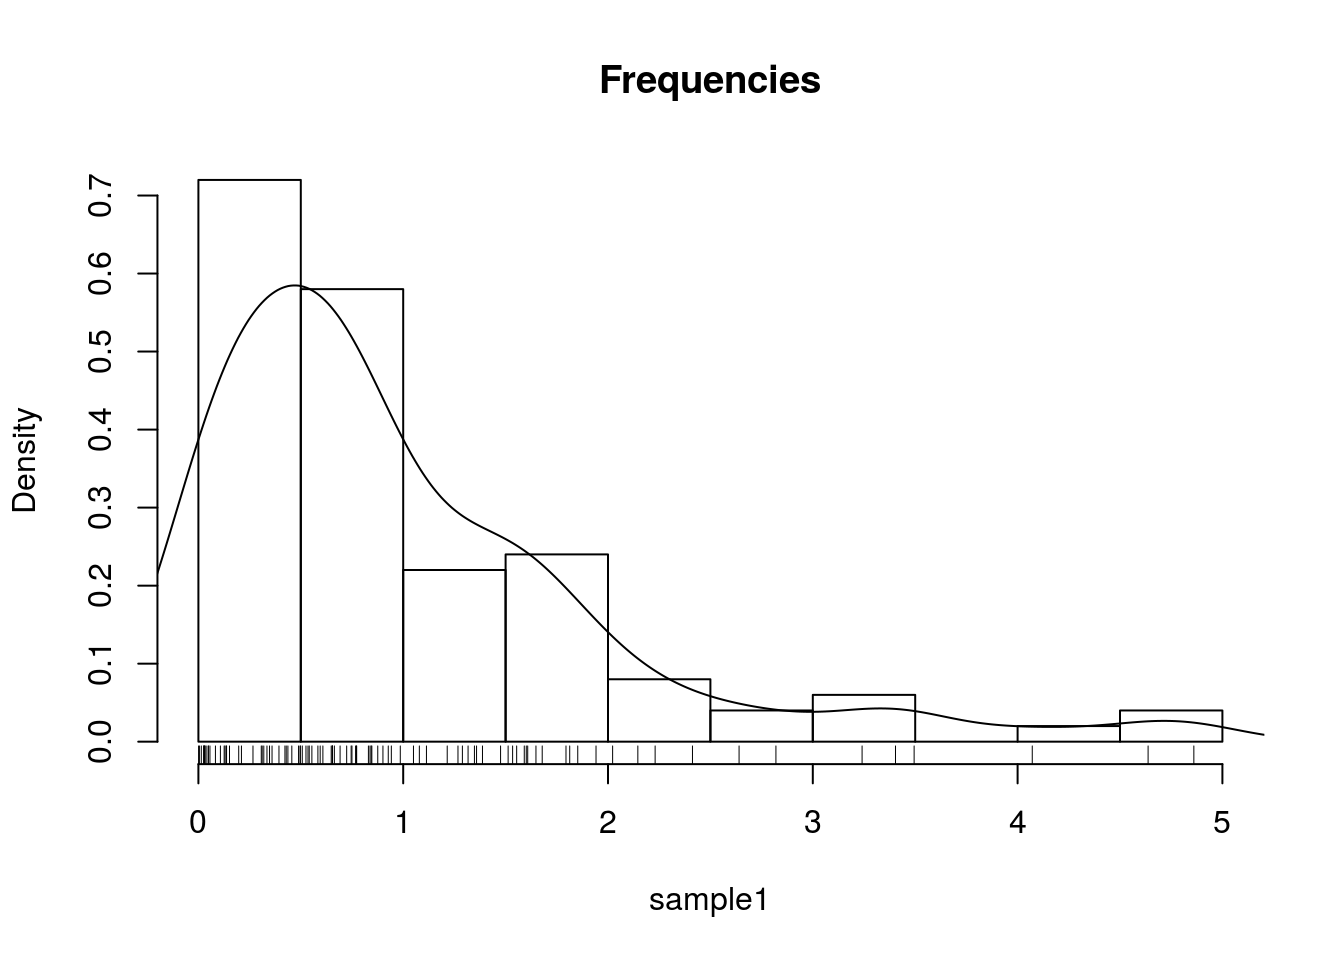
\includegraphics[width=0.5\linewidth]{Rcourse_files/figure-latex/unnamed-chunk-96-1}

The model seems to fit the data nicely. A common measure of the goodness
of fit is the \emph{coefficient of determination}, more commonly known
as the \(R^2\).

\BeginKnitrBlock{definition}
\protect\hypertarget{def:unnamed-chunk-97}{}{\label{def:unnamed-chunk-97}}The
coefficient of determination, denoted \(R^2\), is defined as

\begin{align}
  R^2:= 1-\frac{\sum_i (y_i - \hat y_i)^2}{\sum_i (y_i - \bar y)^2}
\end{align}

Where \(\hat y_i\) is the model's prediction,
\(\hat y_i = x_i \hat \beta\).
\EndKnitrBlock{definition}

It can be easily computed

\begin{Shaded}
\begin{Highlighting}[]
\NormalTok{R2 <-}\StringTok{ }\NormalTok{function(y, y.hat)\{}
  \NormalTok{numerator <-}\StringTok{ }\NormalTok{(y-y.hat)^}\DecValTok{2} \NormalTok\StringTok{ }\NormalTok{sum}
  \NormalTok{denominator <-}\StringTok{ }\NormalTok{(y-}\KeywordTok{mean}\NormalTok{(y))^}\DecValTok{2} \NormalTok\StringTok{ }\NormalTok{sum}
  \DecValTok{1}\NormalTok{-numerator/denominator}
\NormalTok{\}}
\KeywordTok{R2}\NormalTok{(whiteside[whiteside$Insul==}\StringTok{'Before'}\NormalTok{,]$Gas, }\KeywordTok{predict}\NormalTok{(lm}\FloatTok{.1}\NormalTok{))}
\end{Highlighting}
\end{Shaded}

\begin{verbatim}
## [1] 0.9438081
\end{verbatim}

Obviously, R does provide the means to compute something as basic as
\(R^2\), but I will let you find it for yourselves.

\section{Inference}\label{inference}

To perform inference on \(\hat \beta\) in order to test hypotheses and
construct confidence intervals, we need to quantify the uncertainly in
the reported \(\hat \beta\). This is exactly what
Eq.\eqref{eq:ols-distribution} gives us.

Luckily, we don't need to manipulate multivariate distributions
manually, and everything we need is already implemented. The most
important function is \texttt{summary} which gives us an overview of the
model's fit. We emphasize that that fitting a model with \texttt{lm} is
an assumption free algorithmic step. Inference using \texttt{summary} is
\textbf{not} assumption free, and requires the set of assumptions
leading to Eq.\eqref{eq:ols-distribution}.

\begin{Shaded}
\begin{Highlighting}[]
\KeywordTok{summary}\NormalTok{(lm}\FloatTok{.1}\NormalTok{)}
\end{Highlighting}
\end{Shaded}

\begin{verbatim}
## 
## Call:
## lm(formula = Gas ~ Temp, data = whiteside[whiteside$Insul == 
##     "Before", ])
## 
## Residuals:
##      Min       1Q   Median       3Q      Max 
## -0.62020 -0.19947  0.06068  0.16770  0.59778 
## 
## Coefficients:
##             Estimate Std. Error t value Pr(>|t|)    
## (Intercept)  6.85383    0.11842   57.88   <2e-16 ***
## Temp        -0.39324    0.01959  -20.08   <2e-16 ***
## ---
## Signif. codes:  0 '***' 0.001 '**' 0.01 '*' 0.05 '.' 0.1 ' ' 1
## 
## Residual standard error: 0.2813 on 24 degrees of freedom
## Multiple R-squared:  0.9438, Adjusted R-squared:  0.9415 
## F-statistic: 403.1 on 1 and 24 DF,  p-value: < 2.2e-16
\end{verbatim}

Things to note:

\begin{itemize}
\tightlist
\item
  The estimated \(\hat \beta\) is reported in the `Coefficients' table,
  which has point estimates, standard errors, t-statistics, and the
  p-values of a two-sided hypothesis test for each coefficient
  \(H_{0,j}:\beta_j=0, j=1,\dots,p\).
\item
  The \(R^2\) is reported at the bottom. The ``Adjusted R-squared'' is a
  variation that compensates for the model's complexity.
\item
  The original call to \texttt{lm} is saved in the \texttt{Call}
  section.
\item
  Some summary statistics of the residuals (\(y_i-\hat y_i\)) in the
  \texttt{Residuals} section.
\item
  The ``residuals standard error''\footnote{Sometimes known as the Root
    Mean Squared Error (RMSE).} is
  \(\sqrt{(n-p)^{-1} \sum_i (y_i-\hat y_i)^2}\). The ``degrees of
  freedom'' are \(n-p\) which can be thought of as the hardness of the
  problem.
\end{itemize}

As the name suggests, \texttt{summary} is merely a summary. The full
\texttt{summary(lm.1)} object is a monstrous object. Its various
elements can be queried using \texttt{str(sumary(lm.1))}.

Can we check the assumptions required for inference? Some. Let's start
with the linearity assumption. If we were wrong, and the data is not
arranged about a linear line, the residuals will have some shape.

\begin{Shaded}
\begin{Highlighting}[]
\KeywordTok{plot}\NormalTok{(}\KeywordTok{residuals}\NormalTok{(lm}\FloatTok{.1}\NormalTok{)~whiteside[whiteside$Insul==}\StringTok{'Before'}\NormalTok{,]$Temp); }\KeywordTok{abline}\NormalTok{(}\DecValTok{0}\NormalTok{,}\DecValTok{0}\NormalTok{, }\DataTypeTok{lty=}\DecValTok{2}\NormalTok{)}
\end{Highlighting}
\end{Shaded}

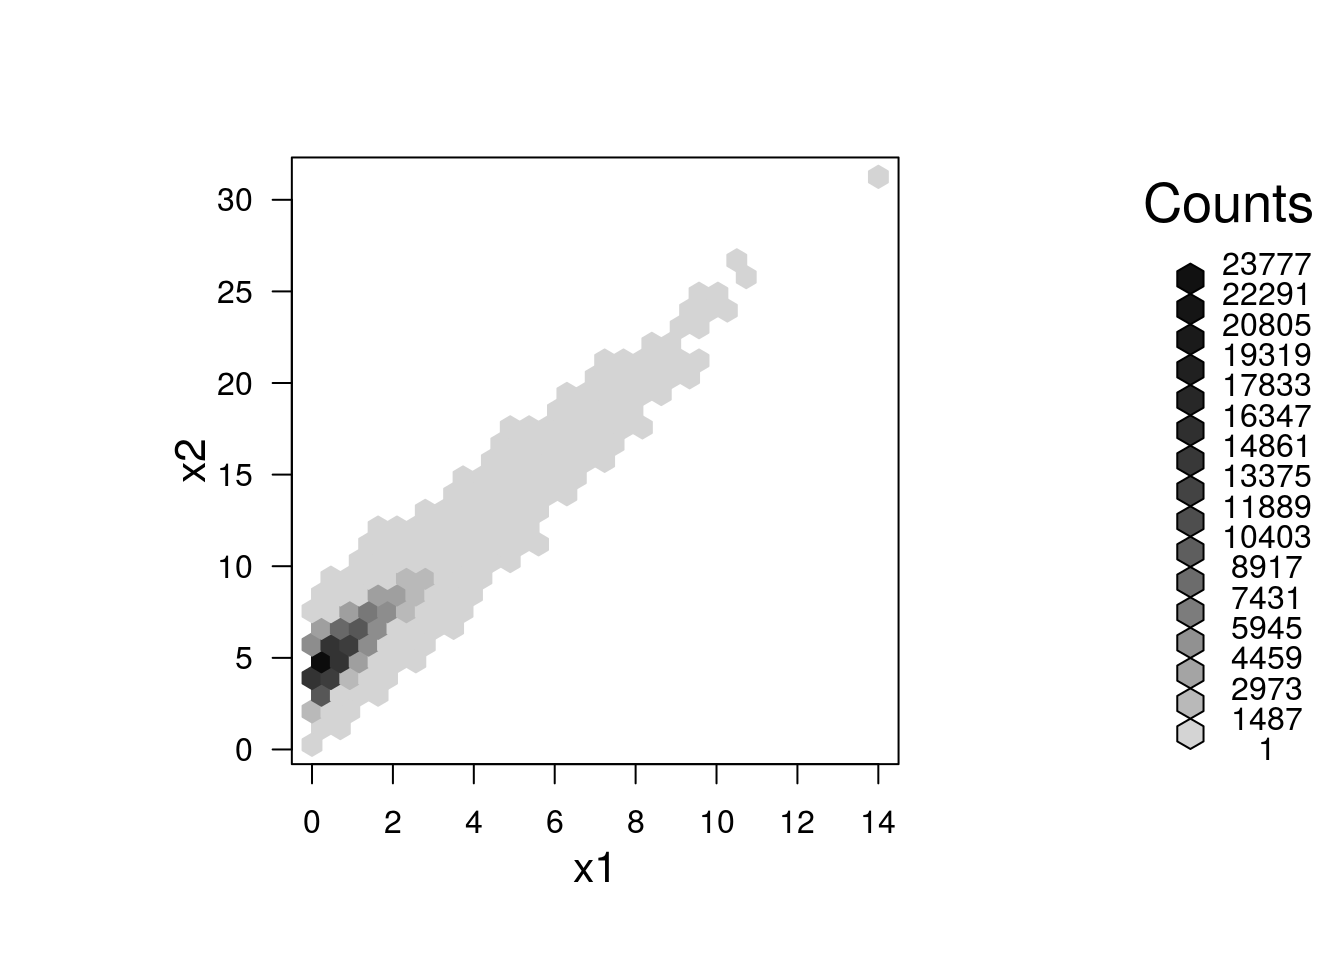
\includegraphics[width=0.5\linewidth]{Rcourse_files/figure-latex/unnamed-chunk-100-1}

I can't say I see any shape. Let's fit a \textbf{wrong} model, just to
see what ``shape'' means.

\begin{Shaded}
\begin{Highlighting}[]
\NormalTok{lm}\FloatTok{.1.1} \NormalTok{<-}\StringTok{ }\KeywordTok{lm}\NormalTok{(Gas~}\KeywordTok{I}\NormalTok{(Temp^}\DecValTok{2}\NormalTok{), }\DataTypeTok{data=}\NormalTok{whiteside[whiteside$Insul==}\StringTok{'Before'}\NormalTok{,])}
\KeywordTok{plot}\NormalTok{(}\KeywordTok{residuals}\NormalTok{(lm}\FloatTok{.1.1}\NormalTok{)~whiteside[whiteside$Insul==}\StringTok{'Before'}\NormalTok{,]$Temp); }\KeywordTok{abline}\NormalTok{(}\DecValTok{0}\NormalTok{,}\DecValTok{0}\NormalTok{, }\DataTypeTok{lty=}\DecValTok{2}\NormalTok{)}
\end{Highlighting}
\end{Shaded}

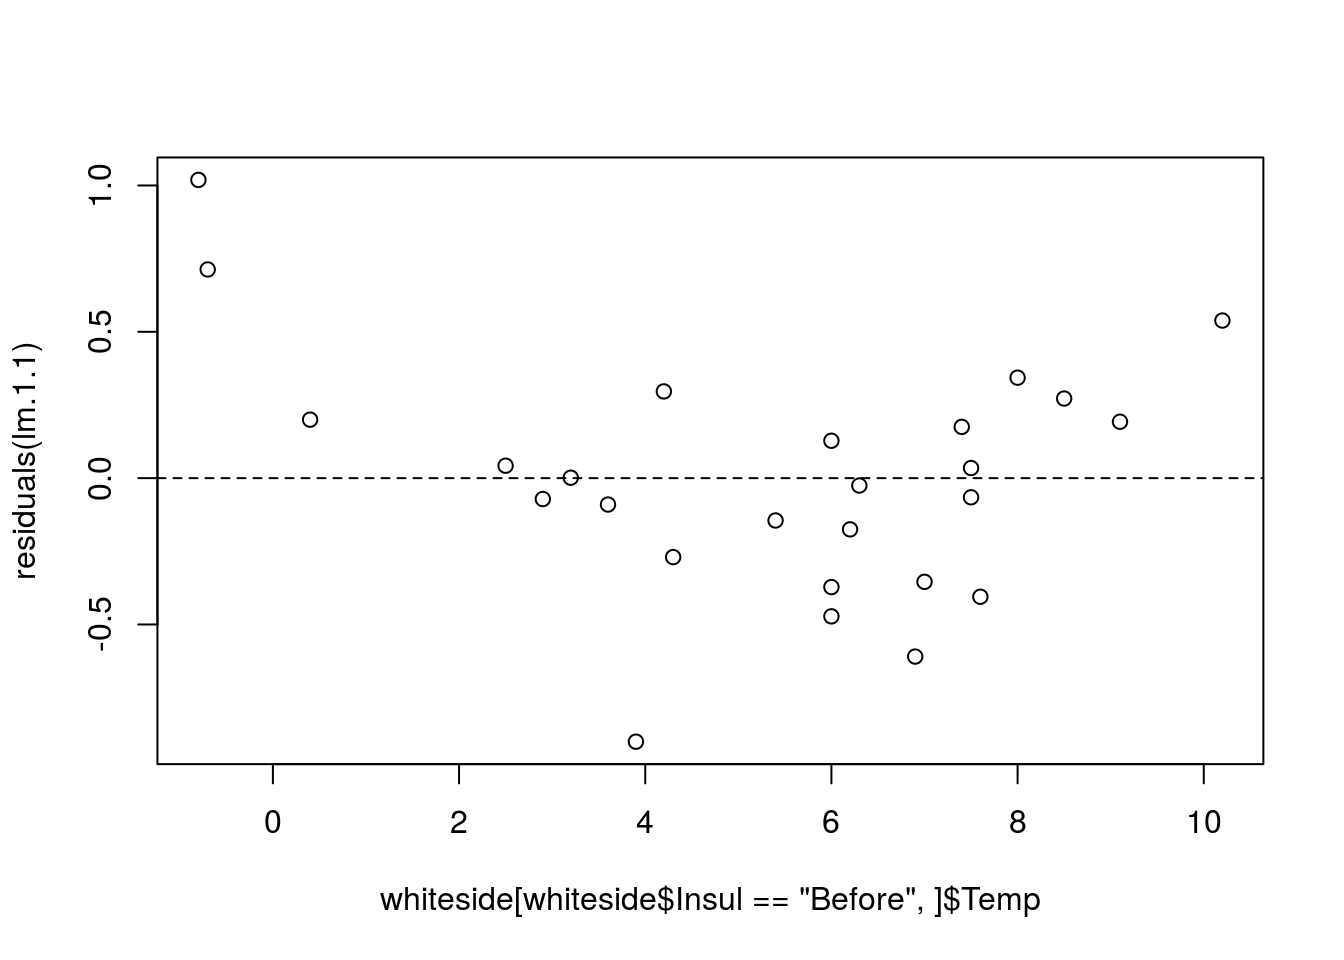
\includegraphics[width=0.5\linewidth]{Rcourse_files/figure-latex/unnamed-chunk-101-1}

Things to note:

\begin{itemize}
\tightlist
\item
  We used \texttt{I(Temp)\^{}2} to specify the model
  \(Gas_i=\beta_0 + \beta_1 Temp^2+ \varepsilon\).
\item
  The residuals have a ``belly''. Because they are not a cloud of noise
  around the linear trend, and we have the wrong model.
\end{itemize}

To the next assumption. We assumed \(\varepsilon_i\) are independent of
everything else. The residuals, \(y_i-\hat y_i\) can be thought of a
sample of \(\varepsilon_i\). When diagnosing the linearity assumption,
we already saw their distribution does not vary with the \(x\)'s,
\texttt{Temp} in our case. They may be correlated with themselves; a
positive departure from the model, may be followed by a series of
positive departures etc. Diagnosing these \emph{auto-correlations} is a
real art, which is not part of our course.

The last assumption we required is normality. As previously stated, if
\(n \gg p\), this assumption is not really needed. If \(n \sim p\),
i.e., \(n\) is in the order of \(p\), we need to verify this assumption.
My favorite tool for this task is the \emph{qqplot}. A qqplot compares
the quantiles of the sample with the respective quantiles of an assumed
distribution. If quantiles align along a line, the assumed distribution
if OK. If quantiles depart from a line, then clearly the assumed
distribution does not fit the sample.

\begin{Shaded}
\begin{Highlighting}[]
\KeywordTok{qqnorm}\NormalTok{(}\KeywordTok{resid}\NormalTok{((lm}\FloatTok{.1}\NormalTok{)))}
\end{Highlighting}
\end{Shaded}

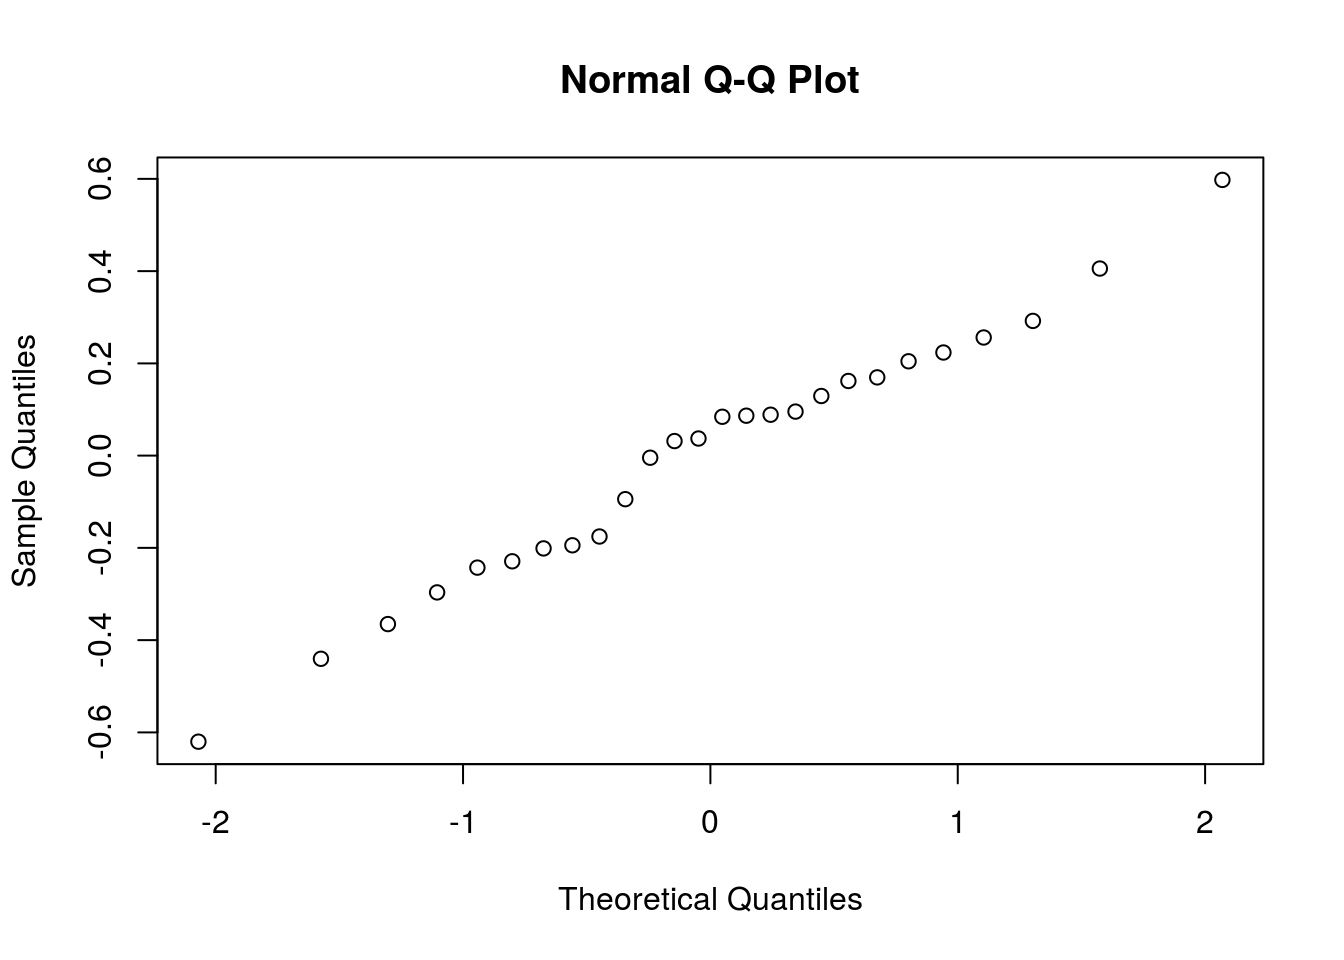
\includegraphics[width=0.5\linewidth]{Rcourse_files/figure-latex/unnamed-chunk-102-1}

The \texttt{qqnorm} function plots a qqplot against a normal
distribution. Judging from the figure, the normality assumption is quite
plausible. Let's try the same on a non-normal sample, namely a uniformly
distributed sample, to see how that would look.

\begin{Shaded}
\begin{Highlighting}[]
\KeywordTok{qqnorm}\NormalTok{(}\KeywordTok{runif}\NormalTok{(}\DecValTok{100}\NormalTok{))}
\end{Highlighting}
\end{Shaded}

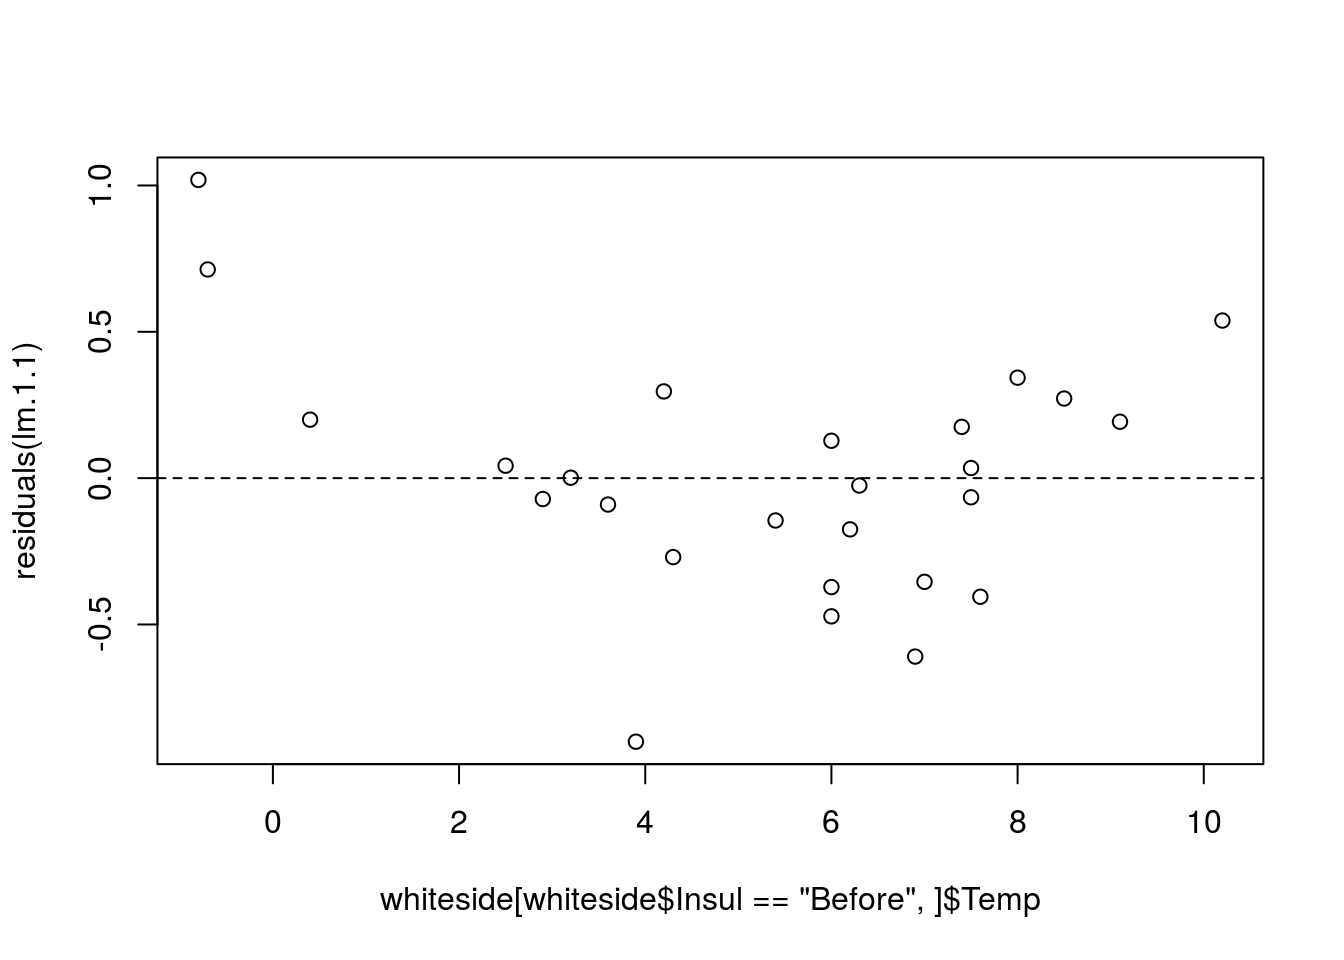
\includegraphics[width=0.5\linewidth]{Rcourse_files/figure-latex/unnamed-chunk-103-1}

\subsection{Testing a Hypothesis on a Single
Coefficient}\label{testing-a-hypothesis-on-a-single-coefficient}

The first inferential test we consider is a hypothesis test on a single
coefficient. In our gas example, we may want to test that the
temperature has no effect on the gas consumption. The answer for that is
given immediately by \texttt{summary(lm.1)}

\begin{Shaded}
\begin{Highlighting}[]
\NormalTok{summary.lm1 <-}\StringTok{ }\KeywordTok{summary}\NormalTok{(lm}\FloatTok{.1}\NormalTok{)}
\NormalTok{coefs.lm1 <-}\StringTok{ }\NormalTok{summary.lm1$coefficients}
\NormalTok{coefs.lm1}
\end{Highlighting}
\end{Shaded}

\begin{verbatim}
##               Estimate Std. Error   t value     Pr(>|t|)
## (Intercept)  6.8538277 0.11842341  57.87561 2.717533e-27
## Temp        -0.3932388 0.01958601 -20.07754 1.640469e-16
\end{verbatim}

We see that the p-value for \(H_{0,1}:\hat \beta_1=0\) against a two
sided alternative is effectively 0.

\subsection{Constructing a Confidence Interval on a Single
Coefficient}\label{constructing-a-confidence-interval-on-a-single-coefficient}

Since the \texttt{summary} function gives us the standard errors of
\(\hat \beta\), we can immediately compute
\(\hat \beta_j \pm 2 \sqrt{Var[\hat \beta_j]}\) to get ourselves a
(roughly) \(95\%\) confidence interval. In our example the interval is

\begin{Shaded}
\begin{Highlighting}[]
\NormalTok{coefs.lm1[}\DecValTok{2}\NormalTok{,}\DecValTok{1}\NormalTok{] +}\StringTok{ }\KeywordTok{c}\NormalTok{(-}\DecValTok{1}\NormalTok{,}\DecValTok{1}\NormalTok{) *}\StringTok{ }\NormalTok{coefs.lm1[}\DecValTok{2}\NormalTok{,}\DecValTok{2}\NormalTok{]}
\end{Highlighting}
\end{Shaded}

\begin{verbatim}
## [1] -0.4128248 -0.3736528
\end{verbatim}

\subsection{Multiple Regression}\label{multiple-regression}

\BeginKnitrBlock{remark}
\iffalse {Remark. } \fi \emph{Multiple regression} is not to be confused
with \emph{multivariate regression} discussed in Chapter
\ref{multivariate}.
\EndKnitrBlock{remark}

The data we now use\footnote{The example is taken from
  \url{http://rtutorialseries.blogspot.co.il/2011/02/r-tutorial-series-two-way-anova-with.html}}
contains a hypothetical sample of \(60\) participants who are divided
into three stress reduction treatment groups (mental, physical, and
medical) and two gender groups (male and female). The stress reduction
values are represented on a scale that ranges from 1 to 5. This dataset
can be conceptualized as a comparison between three stress treatment
programs, one using mental methods, one using physical training, and one
using medication across genders. The values represent how effective the
treatment programs were at reducing participant's stress levels, with
higher numbers indicating higher effectiveness.

\begin{Shaded}
\begin{Highlighting}[]
\NormalTok{data <-}\StringTok{ }\KeywordTok{read.csv}\NormalTok{(}\StringTok{'dataset_anova_twoWay_comparisons.csv'}\NormalTok{)}
\KeywordTok{head}\NormalTok{(data)}
\end{Highlighting}
\end{Shaded}

\begin{verbatim}
##   Treatment   Age StressReduction
## 1    mental young              10
## 2    mental young               9
## 3    mental young               8
## 4    mental   mid               7
## 5    mental   mid               6
## 6    mental   mid               5
\end{verbatim}

How many observations per group?

\begin{Shaded}
\begin{Highlighting}[]
\KeywordTok{table}\NormalTok{(data$Treatment, data$Age)}
\end{Highlighting}
\end{Shaded}

\begin{verbatim}
##           
##            mid old young
##   medical    3   3     3
##   mental     3   3     3
##   physical   3   3     3
\end{verbatim}

Since we have two factorial predictors, this multiple regression is
nothing but a \emph{two way ANOVA}. Let's fit the model and inspect it.

\begin{Shaded}
\begin{Highlighting}[]
\NormalTok{lm}\FloatTok{.2} \NormalTok{<-}\StringTok{ }\KeywordTok{lm}\NormalTok{(StressReduction~.-}\DecValTok{1}\NormalTok{,}\DataTypeTok{data=}\NormalTok{data)}
\KeywordTok{summary}\NormalTok{(lm}\FloatTok{.2}\NormalTok{)}
\end{Highlighting}
\end{Shaded}

\begin{verbatim}
## 
## Call:
## lm(formula = StressReduction ~ . - 1, data = data)
## 
## Residuals:
##    Min     1Q Median     3Q    Max 
##     -1     -1      0      1      1 
## 
## Coefficients:
##                   Estimate Std. Error t value Pr(>|t|)    
## Treatmentmedical    4.0000     0.3892  10.276 7.34e-10 ***
## Treatmentmental     6.0000     0.3892  15.414 2.84e-13 ***
## Treatmentphysical   5.0000     0.3892  12.845 1.06e-11 ***
## Ageold             -3.0000     0.4264  -7.036 4.65e-07 ***
## Ageyoung            3.0000     0.4264   7.036 4.65e-07 ***
## ---
## Signif. codes:  0 '***' 0.001 '**' 0.01 '*' 0.05 '.' 0.1 ' ' 1
## 
## Residual standard error: 0.9045 on 22 degrees of freedom
## Multiple R-squared:  0.9794, Adjusted R-squared:  0.9747 
## F-statistic:   209 on 5 and 22 DF,  p-value: < 2.2e-16
\end{verbatim}

Things to note:

\begin{itemize}
\item
  The \texttt{StressReduction\textasciitilde{}.} syntax is read as
  ``Stress reduction as a function of everything else''.
\item
  The \texttt{StressReduction\textasciitilde{}.-1} means that I do not
  want an intercept in the model, so that the baseline response is 0.
\item
  All the (main) effects seem to be significant.
\item
  The data has 2 factors, but the coefficients table has 4 predictors.
  This is because \texttt{lm} noticed that \texttt{Treatment} and
  \texttt{Age} are factors. Their numerical values are meaningless, and
  it has thus constructed a dummy variable for each level of each
  factor. The names of the effect are a concatenation of the factor's
  name, and its level. You can inspect these dummy variables with the
  \texttt{model.matrix} command.
\end{itemize}

\begin{Shaded}
\begin{Highlighting}[]
\KeywordTok{head}\NormalTok{(}\KeywordTok{model.matrix}\NormalTok{(lm}\FloatTok{.2}\NormalTok{))}
\end{Highlighting}
\end{Shaded}

\begin{verbatim}
##   Treatmentmedical Treatmentmental Treatmentphysical Ageold Ageyoung
## 1                0               1                 0      0        1
## 2                0               1                 0      0        1
## 3                0               1                 0      0        1
## 4                0               1                 0      0        0
## 5                0               1                 0      0        0
## 6                0               1                 0      0        0
\end{verbatim}

If you don't want the default dummy coding, look at \texttt{?contrasts}.

If you are more familiar with the ANOVA literature, or that you don't
want the effects of each level separately, but rather, the effect of
\textbf{all} the levels of each factor, use the \texttt{anova} command.

\begin{Shaded}
\begin{Highlighting}[]
\KeywordTok{anova}\NormalTok{(lm}\FloatTok{.2}\NormalTok{)}
\end{Highlighting}
\end{Shaded}

\begin{verbatim}
## Analysis of Variance Table
## 
## Response: StressReduction
##           Df Sum Sq Mean Sq F value Pr(>F)    
## Treatment  3    693 231.000  282.33 <2e-16 ***
## Age        2    162  81.000   99.00  1e-11 ***
## Residuals 22     18   0.818                   
## ---
## Signif. codes:  0 '***' 0.001 '**' 0.01 '*' 0.05 '.' 0.1 ' ' 1
\end{verbatim}

Things to note:

\begin{itemize}
\tightlist
\item
  The ANOVA table, unlike the \texttt{summary} function, tests if any of
  the levels of a factor has an effect, and not one level at a time.
\item
  The significance of each factor is computed using an F-test.
\item
  The degrees of freedom, encoding the nubmer of levels of a factor, is
  given in the \texttt{Df} column.
\item
  The StressReduction seems to vary for different ages and treatments,
  since both factors are significant.
\end{itemize}

As in any two-way ANOVA, we may want to ask if different age groups
respond differently to different treatments. In the statistical
parlance, this is called an \emph{interaction}, or more precisely, an
\emph{interaction of order 2}.

\begin{Shaded}
\begin{Highlighting}[]
\NormalTok{lm}\FloatTok{.3} \NormalTok{<-}\StringTok{ }\KeywordTok{lm}\NormalTok{(StressReduction~Treatment+Age+Treatment:Age}\DecValTok{-1}\NormalTok{,}\DataTypeTok{data=}\NormalTok{data)}
\end{Highlighting}
\end{Shaded}

The syntax
\texttt{StressReduction\textasciitilde{}Treatment+Age+Treatment:Age-1}
tells R to include main effects of Treatment, Age, and their
interactions. Here are other ways to specify the same model.

\begin{Shaded}
\begin{Highlighting}[]
\NormalTok{lm}\FloatTok{.3} \NormalTok{<-}\StringTok{ }\KeywordTok{lm}\NormalTok{(StressReduction ~}\StringTok{ }\NormalTok{Treatment *}\StringTok{ }\NormalTok{Age -}\StringTok{ }\DecValTok{1}\NormalTok{,}\DataTypeTok{data=}\NormalTok{data)}
\NormalTok{lm}\FloatTok{.3} \NormalTok{<-}\StringTok{ }\KeywordTok{lm}\NormalTok{(StressReduction~(.)^}\DecValTok{2} \NormalTok{-}\StringTok{ }\DecValTok{1}\NormalTok{,}\DataTypeTok{data=}\NormalTok{data)}
\end{Highlighting}
\end{Shaded}

The syntax \texttt{Treatment\ *\ Age} means ``mains effects with second
order interactions''. The syntax \texttt{(.)\^{}2} means ``everything
with second order interactions''

Lets inspect the model

\begin{Shaded}
\begin{Highlighting}[]
\KeywordTok{summary}\NormalTok{(lm}\FloatTok{.3}\NormalTok{)}
\end{Highlighting}
\end{Shaded}

\begin{verbatim}
## 
## Call:
## lm(formula = StressReduction ~ Treatment + Age + Treatment:Age - 
##     1, data = data)
## 
## Residuals:
##    Min     1Q Median     3Q    Max 
##     -1     -1      0      1      1 
## 
## Coefficients:
##                              Estimate Std. Error t value Pr(>|t|)    
## Treatmentmedical            4.000e+00  5.774e-01   6.928 1.78e-06 ***
## Treatmentmental             6.000e+00  5.774e-01  10.392 4.92e-09 ***
## Treatmentphysical           5.000e+00  5.774e-01   8.660 7.78e-08 ***
## Ageold                     -3.000e+00  8.165e-01  -3.674  0.00174 ** 
## Ageyoung                    3.000e+00  8.165e-01   3.674  0.00174 ** 
## Treatmentmental:Ageold      4.246e-16  1.155e+00   0.000  1.00000    
## Treatmentphysical:Ageold    1.034e-15  1.155e+00   0.000  1.00000    
## Treatmentmental:Ageyoung   -3.126e-16  1.155e+00   0.000  1.00000    
## Treatmentphysical:Ageyoung  5.128e-16  1.155e+00   0.000  1.00000    
## ---
## Signif. codes:  0 '***' 0.001 '**' 0.01 '*' 0.05 '.' 0.1 ' ' 1
## 
## Residual standard error: 1 on 18 degrees of freedom
## Multiple R-squared:  0.9794, Adjusted R-squared:  0.9691 
## F-statistic:    95 on 9 and 18 DF,  p-value: 2.556e-13
\end{verbatim}

Things to note:

\begin{itemize}
\tightlist
\item
  There are still \(5\) main effects, but also \(4\) interactions. This
  is because when allowing a different average response for every
  \(Treatment*Age\) combination, we are effectively estimating \(3*3=9\)
  cell means, even if they are not parametrized as cell means, but
  rather as main effect and interactions.
\item
  The interactions do not seem to be significant.
\end{itemize}

Asking if all the interactions are significant, is asking if the
different age groups have the same response to different treatments. Can
we answer that based on the various interactions? We might, but it is
possible that no single interaction is significant, while the
combination is. To test for all the interactions together, we can simply
check if the model without interactions is (significantly) better than a
model with interactions. I.e., compare \texttt{lm.2} to \texttt{lm.3}.
This is done with the \texttt{anova} command.

\begin{Shaded}
\begin{Highlighting}[]
\KeywordTok{anova}\NormalTok{(lm}\FloatTok{.2}\NormalTok{,lm}\FloatTok{.3}\NormalTok{, }\DataTypeTok{test=}\StringTok{'F'}\NormalTok{)}
\end{Highlighting}
\end{Shaded}

\begin{verbatim}
## Analysis of Variance Table
## 
## Model 1: StressReduction ~ (Treatment + Age) - 1
## Model 2: StressReduction ~ Treatment + Age + Treatment:Age - 1
##   Res.Df RSS Df Sum of Sq  F Pr(>F)
## 1     22  18                       
## 2     18  18  4         0  0      1
\end{verbatim}

We see that \texttt{lm.3} is \textbf{not} better than \texttt{lm.2}, so
that we can conclude that there are no interactions: different ages have
the same response to different treatments.

\subsection{Testing a Hypothesis on a Single
Contrast}\label{testing-a-hypothesis-on-a-single-contrast}

Returning to \texttt{lm.2}.

\begin{Shaded}
\begin{Highlighting}[]
\KeywordTok{coef}\NormalTok{(}\KeywordTok{summary}\NormalTok{(lm}\FloatTok{.2}\NormalTok{))}
\end{Highlighting}
\end{Shaded}

\begin{verbatim}
##                   Estimate Std. Error   t value     Pr(>|t|)
## Treatmentmedical         4  0.3892495 10.276186 7.336391e-10
## Treatmentmental          6  0.3892495 15.414279 2.835706e-13
## Treatmentphysical        5  0.3892495 12.845233 1.064101e-11
## Ageold                  -3  0.4264014 -7.035624 4.647299e-07
## Ageyoung                 3  0.4264014  7.035624 4.647299e-07
\end{verbatim}

We see that the effect of the various treatments is rather similar. It
is possible that all treatments actually have the same effect. Comparing
the levels of a factor is called a \emph{contrast}. Let's test if the
medical treatment, has in fact, the same effect as the physical
treatment.

\begin{Shaded}
\begin{Highlighting}[]
\KeywordTok{library}\NormalTok{(multcomp)}
\NormalTok{my.contrast <-}\StringTok{ }\KeywordTok{matrix}\NormalTok{(}\KeywordTok{c}\NormalTok{(-}\DecValTok{1}\NormalTok{,}\DecValTok{0}\NormalTok{,}\DecValTok{1}\NormalTok{,}\DecValTok{0}\NormalTok{,}\DecValTok{0}\NormalTok{), }\DataTypeTok{nrow =}  \DecValTok{1}\NormalTok{)}
\NormalTok{lm}\FloatTok{.4} \NormalTok{<-}\StringTok{ }\KeywordTok{glht}\NormalTok{(lm}\FloatTok{.2}\NormalTok{, }\DataTypeTok{linfct=}\NormalTok{my.contrast)}
\KeywordTok{summary}\NormalTok{(lm}\FloatTok{.4}\NormalTok{)}
\end{Highlighting}
\end{Shaded}

\begin{verbatim}
## 
##   Simultaneous Tests for General Linear Hypotheses
## 
## Fit: lm(formula = StressReduction ~ . - 1, data = data)
## 
## Linear Hypotheses:
##        Estimate Std. Error t value Pr(>|t|)  
## 1 == 0   1.0000     0.4264   2.345   0.0284 *
## ---
## Signif. codes:  0 '***' 0.001 '**' 0.01 '*' 0.05 '.' 0.1 ' ' 1
## (Adjusted p values reported -- single-step method)
\end{verbatim}

Things to note:

\begin{itemize}
\tightlist
\item
  A contrast is a linear function of the coefficients. In our example
  \(H_0:\beta_1-\beta_3=0\), which justifies the construction of
  `my.contrast'.
\item
  We used the \texttt{glht} function (generalized linear hypothesis
  test) from the package \textbf{multcompt}.
\item
  The contrast is significant, i.e., the effect of a medical treatment,
  is different than that of a physical treatment.
\end{itemize}

\section{Bibliographic Notes}\label{bibliographic-notes-3}

Like any other topic in this book, you can consult
\citet{venables2013modern} for more on linear models. For the theory of
linear models, I like \citet{greene2003econometric}.

\chapter{Generalized Linear Models}\label{glm}

\BeginKnitrBlock{example}
\protect\hypertarget{ex:cigarettes}{}{\label{ex:cigarettes}}Consider the
relation between cigarettes smoked, and the occurance of lung cancer. Do
we expect it to be liner? Probably not. Do we expect the variability to
be constant about the trend, be it linear or not? Probably not.
\EndKnitrBlock{example}

\section{Problem Setup}\label{problem-setup-1}

In the Linear Models Chapter \ref{lm}, we assumed the generative process
to be

\begin{align}
  y|x=x'\beta+\varepsilon
  \label{eq:linear-mean-again}
\end{align}

This does not allow for assumingly non-linear relations, nor does it
allow for the variability of \(\varepsilon\) to change with \(x\).
Generalize linear models (GLM), as the name suggests, are a
generalization that allow that.

\BeginKnitrBlock{remark}
\iffalse {Remark. } \fi Do not confuse \emph{generalized linear models}
with \emph{non-linear regression}, or \emph{generalized least squares}.
These are different things, that we will not discuss.
\EndKnitrBlock{remark}

To understand GLM, we recall that with the normality of \(\varepsilon\),
Eq.\eqref{eq:linear-mean-again} implies that \[
 y|x \sim \mathcal{N}(x'\beta, \sigma^2)
\] For Example \ref{ex:cigarettes}, we would like something in the lines
of \[
 y|x \sim Binom(1,p(x))
\] More generally, for some distribution \(F(\theta)\), with a parameter
\(\theta\), we would like

\begin{align}
  y|x \sim F(\theta(x))
\end{align}

Possible examples include

\begin{align}
 y|x &\sim Poisson(\lambda(x)) \\
 y|x &\sim Exp(\lambda(x)) \\
 y|x &\sim \mathcal{N}(\mu(x),\sigma^2(x)) 
\end{align}

GLMs constrain \(\theta\) to be some function, \(g\), of a linear
combination of the \(x\)'s. Formally, \[\theta(x)=g(x'\beta)\], where
\[x'\beta=\beta_0 + \sum_j x_j \beta_j\]. The function \(g\) is called
the \emph{link} function.

\section{Logistic Regression}\label{logistic-regression}

The best known of the GLM class of models is the \emph{logistic
regression} that deals with Binomial, or more precisely, Bernoulli
distributed data. The link function implied by the logistic regression
is the logistic function

\begin{align}
  g(t)=\frac{e^t}{(1+e^t)}
  \label{eq:logistic-link}  
\end{align}

implying that

\begin{align}
  y|x \sim Binom \left( 1, p=\frac{e^{x'\beta}}{1+e^{x'\beta}} \right)
  \label{eq:logistic}
\end{align}

Before we fit such a model, we try to justify this construction, in
particular, this enigmatic link function in Eq.\eqref{eq:logistic-link}.
Let's look at the simplest possible case: the comparison of two groups
indexed by \(x\): \(x=0\) for the first, and \(x=1\) for the second.

\begin{align}
   p(x=0)=P(y=1|x=0) &= \frac{e^{\beta_0}}{(1+e^{\beta_0})} \label{eq:odds-one} \\ 
   \Rightarrow 
   \frac{P(y=1|x=0)}{P(y=0|x=0)} &= e^{\beta_0} \\
   p(x=1)= P(y=1|x=1) &= \frac{e^{\beta_0+\beta_1}}{(1+e^{\beta_0+\beta_1})} \\
   \Rightarrow 
   \frac{P(y=1|x=1)}{P(y=0|x=1)} &= e^{\beta_0+\beta_1} \label{eq:odds-two}\\
   \Rightarrow 
   \frac{P(y=1|x=1)/P(y=0|x=1)}{P(y=1|x=0)/P(y=0|x=0)} 
   &= e^{\beta_1}  \label{eq:odds-ratio} \\
   \Rightarrow 
   \log \frac{P(y=1|x=1)/P(y=0|x=1)}{P(y=1|x=0)/P(y=0|x=0)} &= \beta_1. \label{eq:log-odds-ratio}
\end{align}

The magnitudes in Eqs.\eqref{eq:odds-one} and \eqref{eq:odds-two}, are known
as the \emph{odds}. Odds are the same as probabilities, but instead of
of telling me there is a \(66\%\) of success, they tell me the odds of
success are ``2 to 1''.

The magnitude in Eq.\eqref{eq:odds-ratio} is known as the \emph{odds
ratio}. The odds ratio compares between the probabilities of two groups,
only that it does not compare them in probability scale, but rather in
odds scale.

The magnitude in Eq.\eqref{eq:log-odds-ratio} is known as the \emph{log
odds ratio}. Besides some nice theoretical properties of log odds
ratios, which we will not discuss, they are important since it
demystifies the choice of the link function in \eqref{eq:logistic-link}:
\textbf{it allows us to interpret \(\beta\) of the logistic regression
as the odds-ratios (in log scale)}.

Another popular link function is the normal quantile function, a.k.a.,
the Gaussian inverse CDF, leading to \emph{probit regression} instead of
logistic regression.

\subsection{Logistic Regression with
R}\label{logistic-regression-with-r}

Let's get us some data. The \texttt{PlantGrowth} data records the weight
of plants under three conditions: control, treatment1, and treatment2.

\begin{Shaded}
\begin{Highlighting}[]
\KeywordTok{head}\NormalTok{(PlantGrowth)}
\end{Highlighting}
\end{Shaded}

\begin{verbatim}
##   weight group
## 1   4.17  ctrl
## 2   5.58  ctrl
## 3   5.18  ctrl
## 4   6.11  ctrl
## 5   4.50  ctrl
## 6   4.61  ctrl
\end{verbatim}

We will now \texttt{attach} the data so that its contents is available
in the workspace (don't forget to \texttt{detach} afterwards, or you can
expect some conflicting object names). We will also use the \texttt{cut}
function to create a two-class response variable for Light, and Heavy
plants (we are doing logistic regression, so we need a two-class
response). As a general rule of thumb, when we discretize continuous
variables, we lose information. for pedagogical reasons, however, we
will proceed with this bad practice.

\begin{Shaded}
\begin{Highlighting}[]
\KeywordTok{attach}\NormalTok{(PlantGrowth)}
\NormalTok{weight.factor<-}\StringTok{ }\KeywordTok{cut}\NormalTok{(weight, }\DecValTok{2}\NormalTok{, }\DataTypeTok{labels=}\KeywordTok{c}\NormalTok{(}\StringTok{'Light'}\NormalTok{, }\StringTok{'Heavy'}\NormalTok{))}
\KeywordTok{plot}\NormalTok{(}\KeywordTok{table}\NormalTok{(group, weight.factor))}
\end{Highlighting}
\end{Shaded}

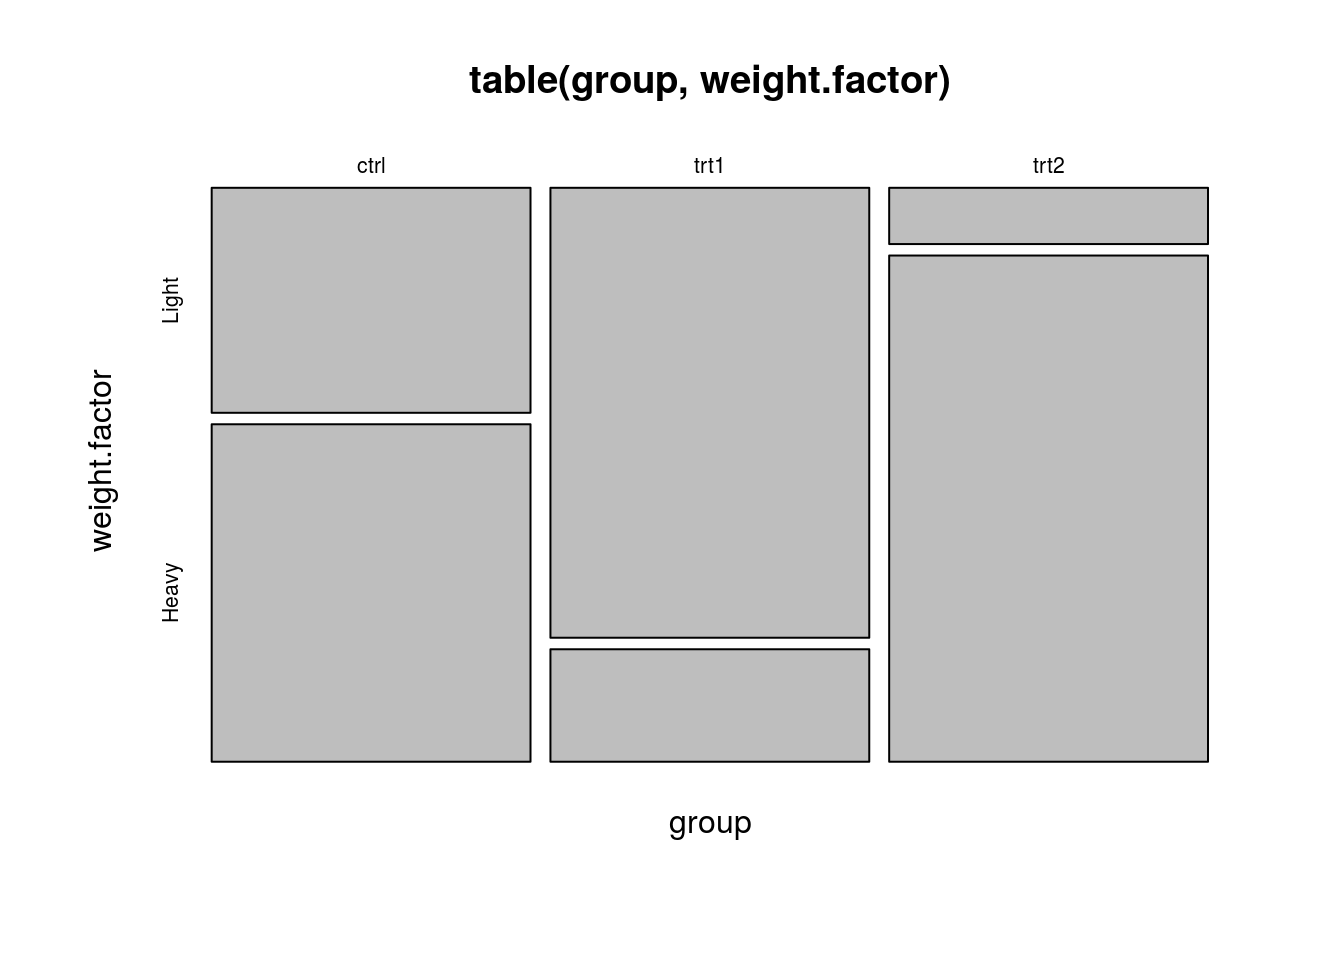
\includegraphics[width=0.5\linewidth]{Rcourse_files/figure-latex/unnamed-chunk-120-1}

Let's fit a logistic regression, and inspect the output.

\begin{Shaded}
\begin{Highlighting}[]
\NormalTok{glm}\FloatTok{.1}\NormalTok{<-}\StringTok{ }\KeywordTok{glm}\NormalTok{(weight.factor~group, }\DataTypeTok{family=}\NormalTok{binomial)}
\KeywordTok{summary}\NormalTok{(glm}\FloatTok{.1}\NormalTok{)}
\end{Highlighting}
\end{Shaded}

\begin{verbatim}
## 
## Call:
## glm(formula = weight.factor ~ group, family = binomial)
## 
## Deviance Residuals: 
##     Min       1Q   Median       3Q      Max  
## -2.1460  -0.6681   0.4590   0.8728   1.7941  
## 
## Coefficients:
##             Estimate Std. Error z value Pr(>|z|)  
## (Intercept)   0.4055     0.6455   0.628   0.5299  
## grouptrt1    -1.7918     1.0206  -1.756   0.0792 .
## grouptrt2     1.7918     1.2360   1.450   0.1471  
## ---
## Signif. codes:  0 '***' 0.001 '**' 0.01 '*' 0.05 '.' 0.1 ' ' 1
## 
## (Dispersion parameter for binomial family taken to be 1)
## 
##     Null deviance: 41.054  on 29  degrees of freedom
## Residual deviance: 29.970  on 27  degrees of freedom
## AIC: 35.97
## 
## Number of Fisher Scoring iterations: 4
\end{verbatim}

Things to note:

\begin{itemize}
\tightlist
\item
  The \texttt{glm} function is our workhorse for all GLM models.
\item
  The \texttt{family} argument of \texttt{glm} tells R the output is
  binomial, thus, performing a logistic regression.
\item
  The \texttt{summary} function is content aware. It gives a different
  output for \texttt{glm} class objects than for other objects, such as
  the \texttt{lm} we saw in Chapter \ref{lm}.
\item
  As usual, we get the coefficients table, but recall that they are to
  be interpreted as (log) odd-ratios.
\item
  As usual, we get the significance for the test of no-effect, versus a
  two-sided alternative.
\item
  The residuals of \texttt{glm} are slightly different than the
  \texttt{lm} residuals, and called \emph{Deviance Residuals}.
\item
  For help see \texttt{?glm}, \texttt{?family}, and
  \texttt{?summary.glm}.
\end{itemize}

Like for linear models, we can use an ANOVA table to check if treatments
have any effect, and not one treatment at a time. In the case of GLMS,
this is called an \emph{analysis of deviance} table.

\begin{Shaded}
\begin{Highlighting}[]
\KeywordTok{anova}\NormalTok{(glm}\FloatTok{.1}\NormalTok{, }\DataTypeTok{test=}\StringTok{'LRT'}\NormalTok{)}
\end{Highlighting}
\end{Shaded}

\begin{verbatim}
## Analysis of Deviance Table
## 
## Model: binomial, link: logit
## 
## Response: weight.factor
## 
## Terms added sequentially (first to last)
## 
## 
##       Df Deviance Resid. Df Resid. Dev Pr(>Chi)   
## NULL                     29     41.054            
## group  2   11.084        27     29.970 0.003919 **
## ---
## Signif. codes:  0 '***' 0.001 '**' 0.01 '*' 0.05 '.' 0.1 ' ' 1
\end{verbatim}

Things to note:

\begin{itemize}
\tightlist
\item
  The \texttt{anova} function, like the \texttt{summary} function, are
  content-aware and produce a different output for the \texttt{glm}
  class than for the \texttt{lm} class.
\item
  In GLMs there is no canonical test (like the F test for \texttt{lm}).
  We thus specify the type of test desired with the \texttt{test}
  argument.
\item
  The distribution of the weights of the plants does vary with the
  treatment given, as we may see from the significance of the
  \texttt{group} factor.
\item
  Readers familiar with ANOVA tables, should know that we computed the
  GLM equivalent of a type I sum- of-squares. Run
  \texttt{drop1(glm.1,\ test=\textquotesingle{}Chisq\textquotesingle{})}
  for a GLM equivalent of a type III sum-of-squares.
\item
  For help see \texttt{?anova.glm}.
\end{itemize}

Let's predict the probability of a heavy plant for each treatment.

\begin{Shaded}
\begin{Highlighting}[]
\KeywordTok{predict}\NormalTok{(glm}\FloatTok{.1}\NormalTok{, }\DataTypeTok{type=}\StringTok{'response'}\NormalTok{)}
\end{Highlighting}
\end{Shaded}

\begin{verbatim}
##   1   2   3   4   5   6   7   8   9  10  11  12  13  14  15  16  17  18 
## 0.6 0.6 0.6 0.6 0.6 0.6 0.6 0.6 0.6 0.6 0.2 0.2 0.2 0.2 0.2 0.2 0.2 0.2 
##  19  20  21  22  23  24  25  26  27  28  29  30 
## 0.2 0.2 0.9 0.9 0.9 0.9 0.9 0.9 0.9 0.9 0.9 0.9
\end{verbatim}

Things to note:

\begin{itemize}
\tightlist
\item
  Like the \texttt{summary} and \texttt{anova} functions, the
  \texttt{predict} function is aware that its input is of \texttt{glm}
  class.
\item
  In GLMs there are many types of predictions. The \texttt{type}
  argument controls which type is returned.
\item
  How do I know we are predicting the probability of a heavy plant, and
  not a light plant? Just run \texttt{contrasts(weight.factor)} to see
  which of the categories of the factor \texttt{weight.factor} is
  encoded as 1, and which as 0.
\item
  For help see \texttt{?predict.glm}.
\end{itemize}

Let's detach the data so it is no longer in our workspace, and object
names do not collide.

\begin{Shaded}
\begin{Highlighting}[]
\KeywordTok{detach}\NormalTok{(PlantGrowth)}
\end{Highlighting}
\end{Shaded}

We gave an example with a factorial (i.e.~discrete) predictor. We can do
the same with multiple continuous predictors.

\begin{Shaded}
\begin{Highlighting}[]
\KeywordTok{data}\NormalTok{(}\StringTok{'Pima.te'}\NormalTok{, }\DataTypeTok{package=}\StringTok{'MASS'}\NormalTok{) }\CommentTok{# Loads data}
\KeywordTok{head}\NormalTok{(Pima.te)}
\end{Highlighting}
\end{Shaded}

\begin{verbatim}
##   npreg glu bp skin  bmi   ped age type
## 1     6 148 72   35 33.6 0.627  50  Yes
## 2     1  85 66   29 26.6 0.351  31   No
## 3     1  89 66   23 28.1 0.167  21   No
## 4     3  78 50   32 31.0 0.248  26  Yes
## 5     2 197 70   45 30.5 0.158  53  Yes
## 6     5 166 72   19 25.8 0.587  51  Yes
\end{verbatim}

\begin{Shaded}
\begin{Highlighting}[]
\NormalTok{glm}\FloatTok{.2}\NormalTok{<-}\StringTok{ }\KeywordTok{step}\NormalTok{(}\KeywordTok{glm}\NormalTok{(type~., }\DataTypeTok{data=}\NormalTok{Pima.te, }\DataTypeTok{family=}\NormalTok{binomial))}
\end{Highlighting}
\end{Shaded}

\begin{verbatim}
## Start:  AIC=301.79
## type ~ npreg + glu + bp + skin + bmi + ped + age
## 
##         Df Deviance    AIC
## - skin   1   286.22 300.22
## - bp     1   286.26 300.26
## - age    1   286.76 300.76
## <none>       285.79 301.79
## - npreg  1   291.60 305.60
## - ped    1   292.15 306.15
## - bmi    1   293.83 307.83
## - glu    1   343.68 357.68
## 
## Step:  AIC=300.22
## type ~ npreg + glu + bp + bmi + ped + age
## 
##         Df Deviance    AIC
## - bp     1   286.73 298.73
## - age    1   287.23 299.23
## <none>       286.22 300.22
## - npreg  1   292.35 304.35
## - ped    1   292.70 304.70
## - bmi    1   302.55 314.55
## - glu    1   344.60 356.60
## 
## Step:  AIC=298.73
## type ~ npreg + glu + bmi + ped + age
## 
##         Df Deviance    AIC
## - age    1   287.44 297.44
## <none>       286.73 298.73
## - npreg  1   293.00 303.00
## - ped    1   293.35 303.35
## - bmi    1   303.27 313.27
## - glu    1   344.67 354.67
## 
## Step:  AIC=297.44
## type ~ npreg + glu + bmi + ped
## 
##         Df Deviance    AIC
## <none>       287.44 297.44
## - ped    1   294.54 302.54
## - bmi    1   303.72 311.72
## - npreg  1   304.01 312.01
## - glu    1   349.80 357.80
\end{verbatim}

\begin{Shaded}
\begin{Highlighting}[]
\KeywordTok{summary}\NormalTok{(glm}\FloatTok{.2}\NormalTok{)}
\end{Highlighting}
\end{Shaded}

\begin{verbatim}
## 
## Call:
## glm(formula = type ~ npreg + glu + bmi + ped, family = binomial, 
##     data = Pima.te)
## 
## Deviance Residuals: 
##     Min       1Q   Median       3Q      Max  
## -2.9845  -0.6462  -0.3661   0.5977   2.5304  
## 
## Coefficients:
##              Estimate Std. Error z value Pr(>|z|)    
## (Intercept) -9.552177   1.096207  -8.714  < 2e-16 ***
## npreg        0.178066   0.045343   3.927  8.6e-05 ***
## glu          0.037971   0.005442   6.978  3.0e-12 ***
## bmi          0.084107   0.021950   3.832 0.000127 ***
## ped          1.165658   0.444054   2.625 0.008664 ** 
## ---
## Signif. codes:  0 '***' 0.001 '**' 0.01 '*' 0.05 '.' 0.1 ' ' 1
## 
## (Dispersion parameter for binomial family taken to be 1)
## 
##     Null deviance: 420.30  on 331  degrees of freedom
## Residual deviance: 287.44  on 327  degrees of freedom
## AIC: 297.44
## 
## Number of Fisher Scoring iterations: 5
\end{verbatim}

Things to note:

\begin{itemize}
\tightlist
\item
  We used the \texttt{\textasciitilde{}.} syntax to tell R to fit a
  model with all the available predictors.
\item
  Since we want to focus on significant predictors, we used the
  \texttt{step} function to perform a \emph{step-wise} regression,
  i.e.~sequentially remove non-significant predictors. The function
  reports each model it has checked, and the variable it has decided to
  remove at each step.
\item
  The output of \texttt{step} is a single model, with the subset of
  significant predictors.
\end{itemize}

\section{Poisson Regression}\label{poisson-regression}

Poisson regression means we fit a model assuming
\(y|x \sim Poisson(\lambda(x))\). Put differently, we assume that for
each treatment, encoded as a combinations of predictors \(x\), the
response is Poisson distributed with a rate that depends on the
predictors.

The typical link function for Poisson regression is \(g(t)=e^t\). This
means that we assume \(y|x \sim Poisson(\lambda(x) = e^{x'\beta})\). Why
is this a good choice? We again resort to the two-group case, encoded by
\(x=1\) and \(x=0\), to understand this model:
\(\lambda(x=1)=e^{\beta_0+\beta_1}=e^{beta_0} \; e^{\beta_1}= \lambda(x=0) \; e^{\beta_1}\).
We thus see that this link function implies that a change in \(x\)
\textbf{multiples} the rate of events. For our example\footnote{Taken
  from
  \url{http://www.theanalysisfactor.com/generalized-linear-models-in-r-part-6-poisson-regression-count-variables/}}
we inspect the number of infected high-school kids, as a function of the
days since the outbreak.

\begin{Shaded}
\begin{Highlighting}[]
\NormalTok{cases <-}\StringTok{  }
\KeywordTok{structure}\NormalTok{(}\KeywordTok{list}\NormalTok{(}\DataTypeTok{Days =} \KeywordTok{c}\NormalTok{(1L, 2L, 3L, 3L, 4L, 4L, 4L, 6L, 7L, 8L, }
\NormalTok{8L, 8L, 8L, 12L, 14L, 15L, 17L, 17L, 17L, 18L, 19L, 19L, 20L, }
\NormalTok{23L, 23L, 23L, 24L, 24L, 25L, 26L, 27L, 28L, 29L, 34L, 36L, 36L, }
\NormalTok{42L, 42L, 43L, 43L, 44L, 44L, 44L, 44L, 45L, 46L, 48L, 48L, 49L, }
\NormalTok{49L, 53L, 53L, 53L, 54L, 55L, 56L, 56L, 58L, 60L, 63L, 65L, 67L, }
\NormalTok{67L, 68L, 71L, 71L, 72L, 72L, 72L, 73L, 74L, 74L, 74L, 75L, 75L, }
\NormalTok{80L, 81L, 81L, 81L, 81L, 88L, 88L, 90L, 93L, 93L, 94L, 95L, 95L, }
\NormalTok{95L, 96L, 96L, 97L, 98L, 100L, 101L, 102L, 103L, 104L, 105L, }
\NormalTok{106L, 107L, 108L, 109L, 110L, 111L, 112L, 113L, 114L, 115L), }
    \DataTypeTok{Students =} \KeywordTok{c}\NormalTok{(6L, 8L, 12L, 9L, 3L, 3L, 11L, 5L, 7L, 3L, 8L, }
    \NormalTok{4L, 6L, 8L, 3L, 6L, 3L, 2L, 2L, 6L, 3L, 7L, 7L, 2L, 2L, 8L, }
    \NormalTok{3L, 6L, 5L, 7L, 6L, 4L, 4L, 3L, 3L, 5L, 3L, 3L, 3L, 5L, 3L, }
    \NormalTok{5L, 6L, 3L, 3L, 3L, 3L, 2L, 3L, 1L, 3L, 3L, 5L, 4L, 4L, 3L, }
    \NormalTok{5L, 4L, 3L, 5L, 3L, 4L, 2L, 3L, 3L, 1L, 3L, 2L, 5L, 4L, 3L, }
    \NormalTok{0L, 3L, 3L, 4L, 0L, 3L, 3L, 4L, 0L, 2L, 2L, 1L, 1L, 2L, 0L, }
    \NormalTok{2L, 1L, 1L, 0L, 0L, 1L, 1L, 2L, 2L, 1L, 1L, 1L, 1L, 0L, 0L, }
    \NormalTok{0L, 1L, 1L, 0L, 0L, 0L, 0L, 0L)), }\DataTypeTok{.Names =} \KeywordTok{c}\NormalTok{(}\StringTok{"Days"}\NormalTok{, }\StringTok{"Students"}
\NormalTok{), }\DataTypeTok{class =} \StringTok{"data.frame"}\NormalTok{, }\DataTypeTok{row.names =} \KeywordTok{c}\NormalTok{(}\OtherTok{NA}\NormalTok{, -109L))}
\KeywordTok{attach}\NormalTok{(cases)}
\end{Highlighting}
\end{Shaded}

\begin{verbatim}
## The following objects are masked from cases (pos = 4):
## 
##     Days, Students
\end{verbatim}

\begin{verbatim}
## The following objects are masked from cases (pos = 6):
## 
##     Days, Students
\end{verbatim}

\begin{verbatim}
## The following objects are masked from cases (pos = 9):
## 
##     Days, Students
\end{verbatim}

\begin{verbatim}
## The following objects are masked from cases (pos = 44):
## 
##     Days, Students
\end{verbatim}

\begin{verbatim}
## The following objects are masked from cases (pos = 49):
## 
##     Days, Students
\end{verbatim}

\begin{Shaded}
\begin{Highlighting}[]
\KeywordTok{head}\NormalTok{(cases) }
\end{Highlighting}
\end{Shaded}

\begin{verbatim}
##   Days Students
## 1    1        6
## 2    2        8
## 3    3       12
## 4    3        9
## 5    4        3
## 6    4        3
\end{verbatim}

And visually:

\begin{Shaded}
\begin{Highlighting}[]
\KeywordTok{plot}\NormalTok{(Days, Students, }\DataTypeTok{xlab =} \StringTok{"DAYS"}\NormalTok{, }\DataTypeTok{ylab =} \StringTok{"STUDENTS"}\NormalTok{, }\DataTypeTok{pch =} \DecValTok{16}\NormalTok{)}
\end{Highlighting}
\end{Shaded}

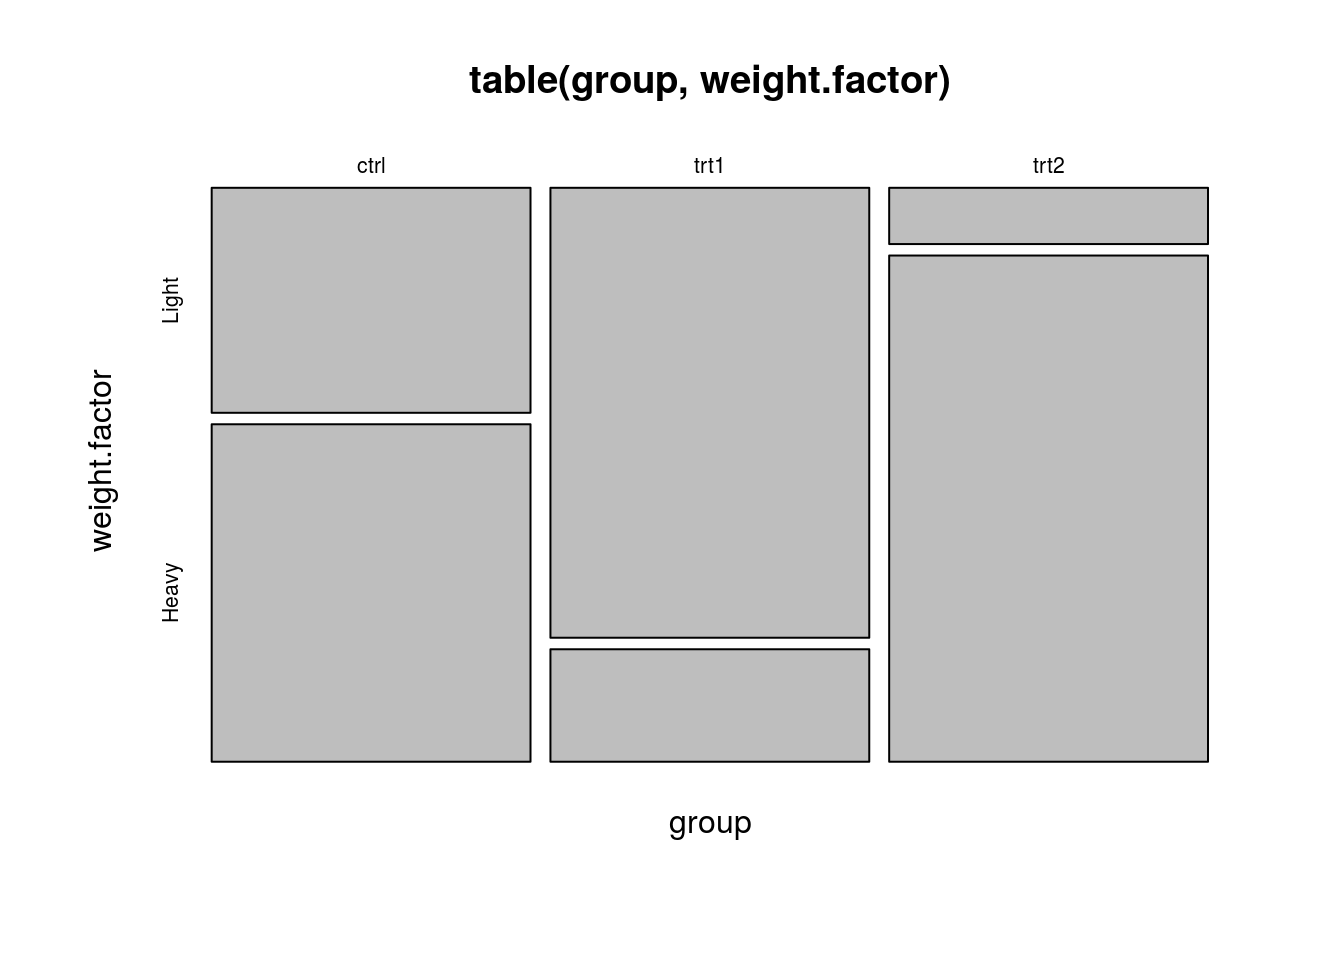
\includegraphics[width=0.5\linewidth]{Rcourse_files/figure-latex/unnamed-chunk-128-1}

We now fit a model to check for the change in the rate of events as a
function of the days since the outbreak.

\begin{Shaded}
\begin{Highlighting}[]
\NormalTok{glm}\FloatTok{.3} \NormalTok{<-}\StringTok{ }\KeywordTok{glm}\NormalTok{(Students ~}\StringTok{ }\NormalTok{Days, }\DataTypeTok{family =} \NormalTok{poisson)}
\KeywordTok{summary}\NormalTok{(glm}\FloatTok{.3}\NormalTok{)}
\end{Highlighting}
\end{Shaded}

\begin{verbatim}
## 
## Call:
## glm(formula = Students ~ Days, family = poisson)
## 
## Deviance Residuals: 
##      Min        1Q    Median        3Q       Max  
## -2.00482  -0.85719  -0.09331   0.63969   1.73696  
## 
## Coefficients:
##              Estimate Std. Error z value Pr(>|z|)    
## (Intercept)  1.990235   0.083935   23.71   <2e-16 ***
## Days        -0.017463   0.001727  -10.11   <2e-16 ***
## ---
## Signif. codes:  0 '***' 0.001 '**' 0.01 '*' 0.05 '.' 0.1 ' ' 1
## 
## (Dispersion parameter for poisson family taken to be 1)
## 
##     Null deviance: 215.36  on 108  degrees of freedom
## Residual deviance: 101.17  on 107  degrees of freedom
## AIC: 393.11
## 
## Number of Fisher Scoring iterations: 5
\end{verbatim}

Things to note:

\begin{itemize}
\tightlist
\item
  We used \texttt{family=poisson} in the \texttt{glm} function to tell R
  that we assume a Poisson distribution.
\item
  The coefficients table is there as usual. When interpreting the table,
  we need to recall that the effect, i.e.~the \(\hat \beta\), are
  \textbf{multiplicative} by assumption.
\item
  Each day \textbf{decreases} the rate of events by a factor of about
  0.02.
\item
  For more information see \texttt{?glm} and \texttt{?family}.
\end{itemize}

\section{Extensions}\label{extensions}

As we already implied, GLMs are a very wide class of models. We do not
need to use the default link function,but more importantly, we are not
constrained to Binomial, or Poisson distributed response. For
exponential, gamma, and other response distributions, see \texttt{?glm}
or the references in the Bibliographic Notes section.

\section{Bibliographic Notes}\label{bibliographic-notes-4}

The ultimate reference on GLMs is \citet{mccullagh1984generalized}. For
a less technical exposition, we refer to the usual
\citet{venables2013modern}.

\chapter{Linear Mixed Models}\label{lme}

\BeginKnitrBlock{example}
\protect\hypertarget{ex:fixed-effects}{}{\label{ex:fixed-effects}}Consider
the problem of testing for a change in the distribution of the bottle
caps produced. Bottle caps are produced by several machines. We could
standardize by removing each machine's average. This first practice
implies the within-machine variability is the only source of
variability. Alternatively, we could ignore the machine of origin. This
second practice implies there are two sources of variability: the
within-machine variability, and the between-machine variability. The
former practice is known as a \emph{fixed effects} model. The latter as
a \emph{random effects} model.
\EndKnitrBlock{example}

\BeginKnitrBlock{example}
\protect\hypertarget{ex:random-effects}{}{\label{ex:random-effects}}Consider
a crossover\footnote{If you are unfamiliar with design of experiments,
  have a look at Chapter 6 of my Quality Engineering
  \href{https://github.com/johnros/qualityEngineering/blob/master/Class_notes/notes.pdf}{class
  notes}.} experimenal design where each subject is given 2 types of
diets, and his/hers health condition is recorded. We could standardize
by removing each subject's average, before comparing the diets (think of
a paired t-test). This first practice implies the within-subject
variability is the only source of variability. Alternatively, we could
ignore the subject of origin. When doing so, we need to recall that
observations from the same subject will be correlated. This second
practice implies there are two sources of variability: the
within-subject variability and the betwee-subject variability.
\EndKnitrBlock{example}

The unifying theme of the above two examples, is that the variability we
want to infer against has several sources. This is typical in mixed
models, which are so popular, that they have earned many names:

\begin{itemize}
\tightlist
\item
  \textbf{Mixed Effects}: Because we may have both \emph{fixed effects}
  we want to estimate and remove, and \emph{random effects} which
  contribute to the variability.
\item
  \textbf{Variance Components}: Because as the examples show, variance
  has more than a single source (like in the Linear Models of Chapter
  \ref{lm}).
\item
  \textbf{Hirarchial Models}: Because as Example \ref{ex:random-effects}
  demonstrates, we can think of the sampling as hierarchical-- first
  sample a subject, and then sample its response.
\item
  \textbf{Repeated Measures}: Because we many have several measurements
  from each unit, like in \ref{ex:random-effects}.
\item
  \textbf{Longitudinal Data}: Because we follow units over time, like in
  Example \ref{ex:random-effects}.
\item
  \textbf{Panel Data}: Is the term typically used in econometric for
  such longitudinal data.
\end{itemize}

We now emphasize:

\begin{enumerate}
\def\labelenumi{\arabic{enumi}.}
\tightlist
\item
  Mixed effect models are a way to infer against the right level of
  variability. Using a naive linear model (which assumes a single source
  of variability) instead of a mixed effects model, probably means your
  inference is overly anti-conservative, i.e., error rates are higher
  than you think.
\item
  A mixed effect models, as we will later see, is typically specified
  via its fixed and random effects. It is possible, however, to specify
  a mixed effects model by putting all the fixed effects into a linear
  model, and putting all the random effects into the covariance between
  \(\varepsilon\). For more on this view, see Chapter 8 in (the
  excellent) \citet{weiss2005modeling}.
\item
  Like in previous chapters, by ``model'' we refer to the assumed
  generative distribution, i.e., the sampling distribution.
\item
  If you are using the model merely for predictions, and not for
  inference on the fixed effects or variance components, then stating
  the generative distribution may be be useful, but not necessarily. See
  the Supervised Learning Chapter \ref{supervised} for more on
  prediction problems.
\end{enumerate}

\section{Problem Setup}\label{problem-setup-2}

\begin{align}
  y|x,u = x'\beta + z'u + \varepsilon
  \label{eq:mixed-model}  
\end{align}

where \(x\) are the factor with fixed effects, \(\beta\) which we may
want to study. The factors \(z\), with effects \(u\), are the random
effects which contribute to variability. Put differently, we state
\(y|x,u\) merely as a convenient way to do inference on \(y|x\), instead
of directly specifying \(Var[y|x]\) as a function of \(u\).

Given a sample of \(n\) observations \((y_i,x_i,z_i)\) from model
\eqref{eq:mixed-model}, we will want to estimate \((\beta,u)\). Under some
assumption on the distribution of \(\varepsilon\) and \(z\), we can use
\emph{maximum likelihood} (ML). In the context of mixed-models, however,
ML is typically replaced with \emph{restricted maximum likelihood}
(ReML), because it returns unbiased estimates of \(Var[y|x]\) and ML
does not.

\section{Mixed Models with R}\label{mixed-models-with-r}

We will fit mixed models with the \texttt{lmer} function from the
\textbf{lme4} package. We start with a small simulation demonstrating
the importance of acknowledging your sources of variability.

\begin{Shaded}
\begin{Highlighting}[]
\NormalTok{n.groups <-}\StringTok{ }\DecValTok{10}
\NormalTok{n.repeats <-}\StringTok{ }\DecValTok{2}
\NormalTok{groups <-}\StringTok{ }\KeywordTok{gl}\NormalTok{(}\DataTypeTok{n =} \NormalTok{n.groups, }\DataTypeTok{k =} \NormalTok{n.repeats)}
\NormalTok{n <-}\StringTok{ }\KeywordTok{length}\NormalTok{(groups)}
\NormalTok{z0 <-}\StringTok{ }\KeywordTok{rnorm}\NormalTok{(}\DecValTok{10}\NormalTok{,}\DecValTok{0}\NormalTok{,}\DecValTok{10}\NormalTok{)}
\NormalTok{z <-}\StringTok{ }\NormalTok{z0[}\KeywordTok{as.numeric}\NormalTok{(groups)] }\CommentTok{# create the random effect vector.}
\NormalTok{epsilon <-}\StringTok{ }\KeywordTok{rnorm}\NormalTok{(n,}\DecValTok{0}\NormalTok{,}\DecValTok{1}\NormalTok{) }\CommentTok{# create the measurement error vector.}
\NormalTok{beta0 <-}\StringTok{ }\DecValTok{2} \CommentTok{# create the global mean}
\NormalTok{y <-}\StringTok{ }\NormalTok{beta0 +}\StringTok{ }\NormalTok{z  +}\StringTok{ }\NormalTok{epsilon }\CommentTok{# generate synthetic sample}
\NormalTok{lm}\FloatTok{.5} \NormalTok{<-}\StringTok{ }\KeywordTok{lm}\NormalTok{(y~z)  }\CommentTok{# fit a linear model}
\KeywordTok{library}\NormalTok{(lme4)}
\NormalTok{lme}\FloatTok{.5} \NormalTok{<-}\StringTok{ }\KeywordTok{lmer}\NormalTok{(y~}\DecValTok{1}\NormalTok{|z) }\CommentTok{# fit a mixed-model}
\end{Highlighting}
\end{Shaded}

The summary of the linear model

\begin{Shaded}
\begin{Highlighting}[]
\NormalTok{summary.lm}\FloatTok{.5} \NormalTok{<-}\StringTok{ }\KeywordTok{summary}\NormalTok{(lm}\FloatTok{.5}\NormalTok{)}
\NormalTok{summary.lm}\FloatTok{.5}
\end{Highlighting}
\end{Shaded}

\begin{verbatim}
## 
## Call:
## lm(formula = y ~ z)
## 
## Residuals:
##     Min      1Q  Median      3Q     Max 
## -1.8115 -0.4222  0.2243  0.3970  2.8710 
## 
## Coefficients:
##             Estimate Std. Error t value Pr(>|t|)    
## (Intercept)   1.8614     0.2397   7.764 3.75e-07 ***
## z             0.9770     0.0225  43.422  < 2e-16 ***
## ---
## Signif. codes:  0 '***' 0.001 '**' 0.01 '*' 0.05 '.' 0.1 ' ' 1
## 
## Residual standard error: 1.031 on 18 degrees of freedom
## Multiple R-squared:  0.9905, Adjusted R-squared:   0.99 
## F-statistic:  1885 on 1 and 18 DF,  p-value: < 2.2e-16
\end{verbatim}

The summary of the mixed-model

\begin{Shaded}
\begin{Highlighting}[]
\NormalTok{summary.lme}\FloatTok{.5} \NormalTok{<-}\StringTok{ }\KeywordTok{summary}\NormalTok{(lme}\FloatTok{.5}\NormalTok{)}
\NormalTok{summary.lme}\FloatTok{.5}
\end{Highlighting}
\end{Shaded}

\begin{verbatim}
## Linear mixed model fit by REML ['lmerMod']
## Formula: y ~ 1 | z
## 
## REML criterion at convergence: 109.7
## 
## Scaled residuals: 
##      Min       1Q   Median       3Q      Max 
## -1.90939 -0.18185  0.03551  0.17218  1.73061 
## 
## Random effects:
##  Groups   Name        Variance Std.Dev.
##  z        (Intercept) 110.725  10.523  
##  Residual               1.515   1.231  
## Number of obs: 20, groups:  z, 10
## 
## Fixed effects:
##             Estimate Std. Error t value
## (Intercept)    4.733      3.339   1.417
\end{verbatim}

Look at the standard error of the global mean, i.e., the intercept: for
\texttt{lm} it is 0.2397539, and for \texttt{lme} it is
\texttt{summary.lme.5\$coefficients{[}1,2{]}}. Why this difference?
Because \texttt{lm} discounts the group effect, while it should treat it
as another source of variability. Clearly, inference using \texttt{lm}
is overly optimistic.

\subsection{A Single Random Effect}\label{a-single-random-effect}

We will use the \texttt{Dyestuff} data from the package, which encodes
the yield, in grams, of a coloring solution (dyestuff), produced in 6
batches using 5 different preparations.

\begin{Shaded}
\begin{Highlighting}[]
\KeywordTok{data}\NormalTok{(Dyestuff, }\DataTypeTok{package=}\StringTok{'lme4'}\NormalTok{)}
\KeywordTok{attach}\NormalTok{(Dyestuff)}
\KeywordTok{head}\NormalTok{(Dyestuff)}
\end{Highlighting}
\end{Shaded}

\begin{verbatim}
##   Batch Yield
## 1     A  1545
## 2     A  1440
## 3     A  1440
## 4     A  1520
## 5     A  1580
## 6     B  1540
\end{verbatim}

And visually

\begin{Shaded}
\begin{Highlighting}[]
\KeywordTok{plot}\NormalTok{(Yield~Batch)}
\end{Highlighting}
\end{Shaded}

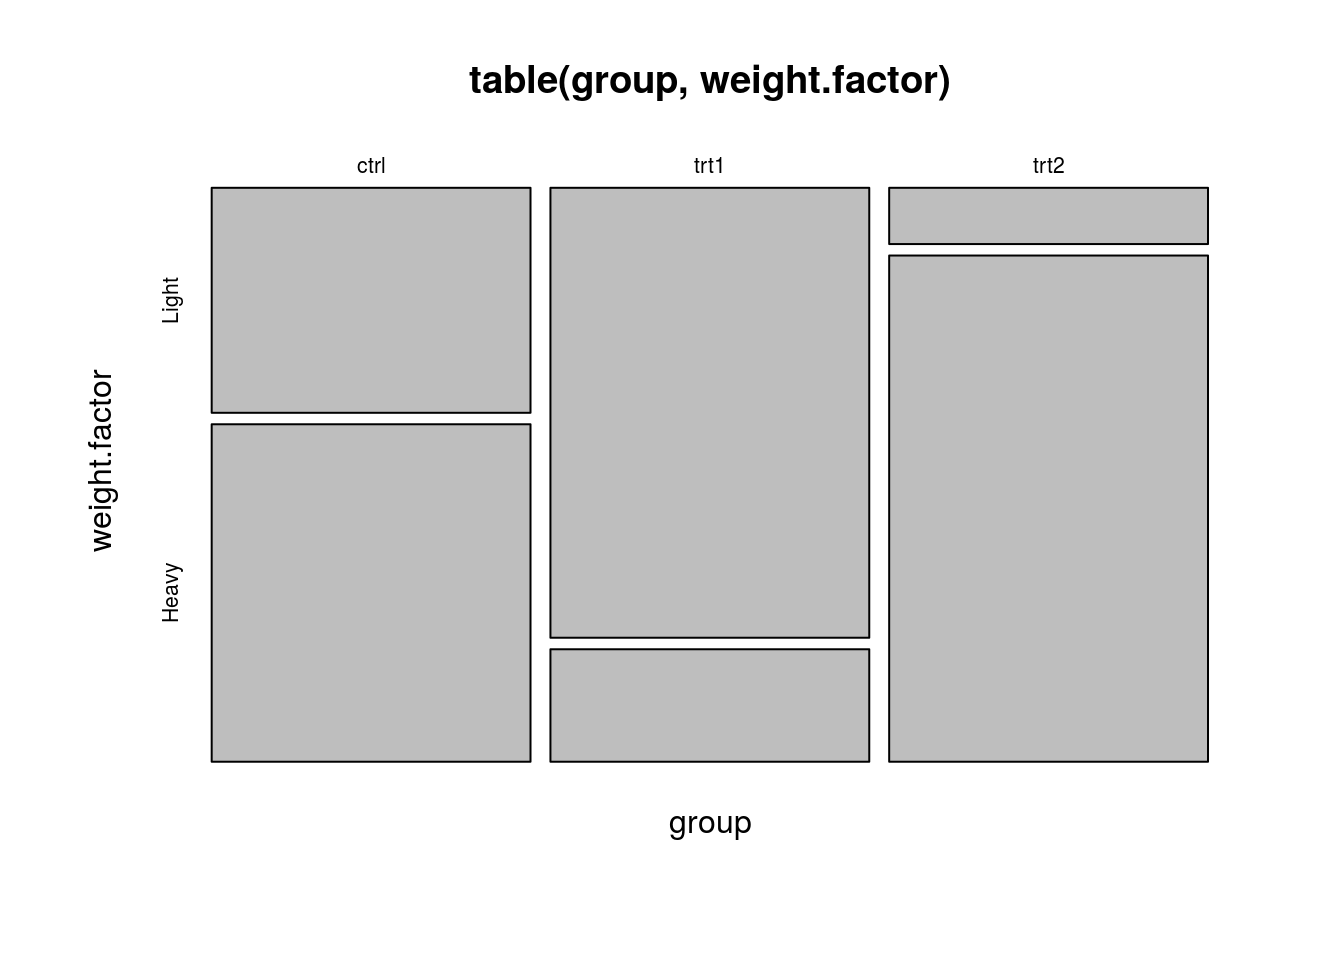
\includegraphics[width=0.5\linewidth]{Rcourse_files/figure-latex/unnamed-chunk-131-1}

If we want to do inference on the mean yield, we need to account for the
two sources of variability: the batch effect, and the measurement error.
We thus fit a mixed model, with an intercept and random batch effect
(which means this is it not a bona-fide mixed-model, but rather, a
simple random-effect model).

\begin{Shaded}
\begin{Highlighting}[]
\NormalTok{lme}\FloatTok{.1}\NormalTok{<-}\StringTok{ }\KeywordTok{lmer}\NormalTok{( Yield ~}\StringTok{ }\DecValTok{1}  \NormalTok{|}\StringTok{ }\NormalTok{Batch  , Dyestuff )}
\KeywordTok{summary}\NormalTok{(lme}\FloatTok{.1}\NormalTok{)}
\end{Highlighting}
\end{Shaded}

\begin{verbatim}
## Linear mixed model fit by REML ['lmerMod']
## Formula: Yield ~ 1 | Batch
##    Data: Dyestuff
## 
## REML criterion at convergence: 319.7
## 
## Scaled residuals: 
##     Min      1Q  Median      3Q     Max 
## -1.4117 -0.7634  0.1418  0.7792  1.8296 
## 
## Random effects:
##  Groups   Name        Variance Std.Dev.
##  Batch    (Intercept) 1764     42.00   
##  Residual             2451     49.51   
## Number of obs: 30, groups:  Batch, 6
## 
## Fixed effects:
##             Estimate Std. Error t value
## (Intercept)  1527.50      19.38    78.8
\end{verbatim}

Things to note:

\begin{itemize}
\tightlist
\item
  As usual, \texttt{summary} is content aware and has a different
  behavior for \texttt{lme} class objects.
\item
  The syntax \texttt{Yield\ \textasciitilde{}\ 1\ \ \textbar{}\ Batch}
  tells R to fit a model with a global intercept (\texttt{1}) and a
  random Batch effect (\texttt{\textbar{}Batch}). More on that later.
\item
  The output distinguishes between random effects, a source of
  variability, and fixed effect, white's coefficients we want to study.
\item
  Were we not interested in the variance components, an (almost)
  equivalent \texttt{lm} formulation is
  \texttt{lm(Yield\ \textasciitilde{}\ Batch)}.
\end{itemize}

Some utility functions let us query the \texttt{lme} object. The
function \texttt{coef} will work, but will return a cumbersome output.
Better use \texttt{fixef} to extract the fixed effects, and
\texttt{ranef} to extract the random effects. The model matrix (of the
fixed effects alone), can be extracted with \texttt{model.matrix}, and
predictions made with \texttt{predict}. Note, however, that predictions
with mixed-effect models are (i) a delicate matter, and (ii) better
treated as prediction problems as in the Supervised Learning Chapter
\ref{supervised}.

\subsection{Several Random Effects}\label{several-random-effects}

Let's make things more interesting. In the \texttt{Penicillin} data, we
measured the diameter of spread of an organism, along the plate used (a
to x), and penicillin type (A to F).

\begin{Shaded}
\begin{Highlighting}[]
\KeywordTok{detach}\NormalTok{(Dyestuff)}
\KeywordTok{head}\NormalTok{(Penicillin)}
\end{Highlighting}
\end{Shaded}

\begin{verbatim}
##   diameter plate sample
## 1       27     a      A
## 2       23     a      B
## 3       26     a      C
## 4       23     a      D
## 5       23     a      E
## 6       21     a      F
\end{verbatim}

One sample per combination:

\begin{Shaded}
\begin{Highlighting}[]
\KeywordTok{attach}\NormalTok{(Penicillin)}
\end{Highlighting}
\end{Shaded}

\begin{verbatim}
## The following objects are masked from Penicillin (pos = 4):
## 
##     diameter, plate, sample
\end{verbatim}

\begin{verbatim}
## The following objects are masked from Penicillin (pos = 6):
## 
##     diameter, plate, sample
\end{verbatim}

\begin{verbatim}
## The following objects are masked from Penicillin (pos = 9):
## 
##     diameter, plate, sample
\end{verbatim}

\begin{verbatim}
## The following objects are masked from Penicillin (pos = 44):
## 
##     diameter, plate, sample
\end{verbatim}

\begin{verbatim}
## The following objects are masked from Penicillin (pos = 47):
## 
##     diameter, plate, sample
\end{verbatim}

\begin{Shaded}
\begin{Highlighting}[]
\KeywordTok{table}\NormalTok{(sample, plate)}
\end{Highlighting}
\end{Shaded}

\begin{verbatim}
##       plate
## sample a b c d e f g h i j k l m n o p q r s t u v w x
##      A 1 1 1 1 1 1 1 1 1 1 1 1 1 1 1 1 1 1 1 1 1 1 1 1
##      B 1 1 1 1 1 1 1 1 1 1 1 1 1 1 1 1 1 1 1 1 1 1 1 1
##      C 1 1 1 1 1 1 1 1 1 1 1 1 1 1 1 1 1 1 1 1 1 1 1 1
##      D 1 1 1 1 1 1 1 1 1 1 1 1 1 1 1 1 1 1 1 1 1 1 1 1
##      E 1 1 1 1 1 1 1 1 1 1 1 1 1 1 1 1 1 1 1 1 1 1 1 1
##      F 1 1 1 1 1 1 1 1 1 1 1 1 1 1 1 1 1 1 1 1 1 1 1 1
\end{verbatim}

And visually:

\begin{Shaded}
\begin{Highlighting}[]
\NormalTok{lattice::}\KeywordTok{dotplot}\NormalTok{(}\KeywordTok{reorder}\NormalTok{(plate, diameter) ~}\StringTok{ }\NormalTok{diameter,}\DataTypeTok{data=}\NormalTok{Penicillin,}
              \DataTypeTok{groups =} \NormalTok{sample,}
              \DataTypeTok{ylab =} \StringTok{"Plate"}\NormalTok{, }\DataTypeTok{xlab =} \StringTok{"Diameter of growth inhibition zone (mm)"}\NormalTok{,}
              \DataTypeTok{type =} \KeywordTok{c}\NormalTok{(}\StringTok{"p"}\NormalTok{, }\StringTok{"a"}\NormalTok{), }\DataTypeTok{auto.key =} \KeywordTok{list}\NormalTok{(}\DataTypeTok{columns =} \DecValTok{6}\NormalTok{, }\DataTypeTok{lines =} \OtherTok{TRUE}\NormalTok{))}
\end{Highlighting}
\end{Shaded}

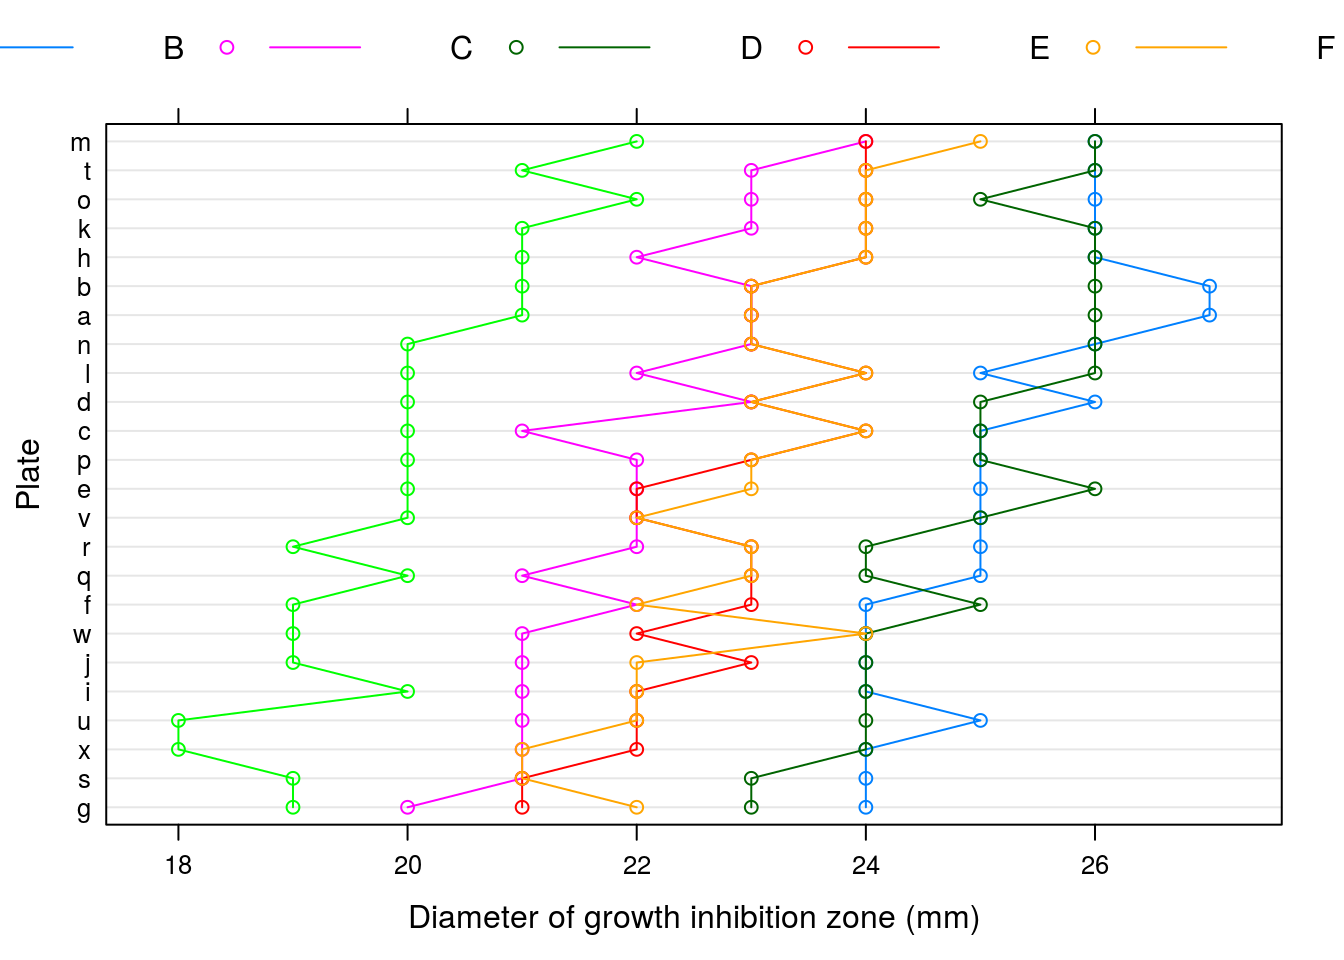
\includegraphics[width=0.5\linewidth]{Rcourse_files/figure-latex/unnamed-chunk-134-1}

Let's fit a mixed-effects model with a random plate effect, and a random
sample effect:

\begin{Shaded}
\begin{Highlighting}[]
\NormalTok{lme}\FloatTok{.2} \NormalTok{<-}\StringTok{ }\KeywordTok{lmer} \NormalTok{( diameter ~}\StringTok{  }\DecValTok{1}\NormalTok{+}\StringTok{ }\NormalTok{(}\DecValTok{1}\NormalTok{|}\StringTok{ }\NormalTok{plate ) +}\StringTok{ }\NormalTok{(}\DecValTok{1}\NormalTok{|}\StringTok{ }\NormalTok{sample ) , Penicillin )}
\KeywordTok{fixef}\NormalTok{(lme}\FloatTok{.2}\NormalTok{) }\CommentTok{# Fixed effects}
\end{Highlighting}
\end{Shaded}

\begin{verbatim}
## (Intercept) 
##    22.97222
\end{verbatim}

\begin{Shaded}
\begin{Highlighting}[]
\KeywordTok{ranef}\NormalTok{(lme}\FloatTok{.2}\NormalTok{) }\CommentTok{# Random effects}
\end{Highlighting}
\end{Shaded}

\begin{verbatim}
## $plate
##   (Intercept)
## a  0.80454704
## b  0.80454704
## c  0.18167191
## d  0.33739069
## e  0.02595313
## f -0.44120322
## g -1.37551591
## h  0.80454704
## i -0.75264078
## j -0.75264078
## k  0.96026582
## l  0.49310948
## m  1.42742217
## n  0.49310948
## o  0.96026582
## p  0.02595313
## q -0.28548443
## r -0.28548443
## s -1.37551591
## t  0.96026582
## u -0.90835956
## v -0.28548443
## w -0.59692200
## x -1.21979713
## 
## $sample
##   (Intercept)
## A  2.18705797
## B -1.01047615
## C  1.93789946
## D -0.09689497
## E -0.01384214
## F -3.00374417
\end{verbatim}

Things to note:

\begin{itemize}
\tightlist
\item
  The syntax
  \texttt{1+\ (1\textbar{}\ plate\ )\ +\ (1\textbar{}\ sample\ )} fits a
  global intercept (mean), a random plate effect, and a random sample
  effect.
\item
  Were we not interested in the variance components, an (almost)
  equivalent \texttt{lm} formulation is
  \texttt{lm(diameter\ \textasciitilde{}\ plate\ +\ sample)}.
\end{itemize}

Since we have two random effect, we may compute the variability of the
global mean (the only fixed effect) as we did before. Perhaps more
interestingly, we can compute the variability in the response, for a
particular plate or sample type.

\begin{Shaded}
\begin{Highlighting}[]
\NormalTok{random.effect.lme2 <-}\StringTok{ }\KeywordTok{ranef}\NormalTok{(lme}\FloatTok{.2}\NormalTok{, }\DataTypeTok{condVar =} \OtherTok{TRUE}\NormalTok{) }
\NormalTok{qrr2 <-}\StringTok{ }\NormalTok{lattice::}\KeywordTok{dotplot}\NormalTok{(random.effect.lme2, }\DataTypeTok{strip =} \OtherTok{FALSE}\NormalTok{)}
\end{Highlighting}
\end{Shaded}

Things to note:

\begin{itemize}
\tightlist
\item
  The \texttt{condVar} argument of the \texttt{ranef} function tells R
  to compute the variability in response conditional on each random
  effect at a time.
\item
  The \texttt{dotplot} function, from the \textbf{lattice} package, is
  only there for the fancy plotting.
\end{itemize}

Variability in response for each plate, over various sample types:

\begin{Shaded}
\begin{Highlighting}[]
\KeywordTok{print}\NormalTok{(qrr2[[}\DecValTok{1}\NormalTok{]]) }
\end{Highlighting}
\end{Shaded}

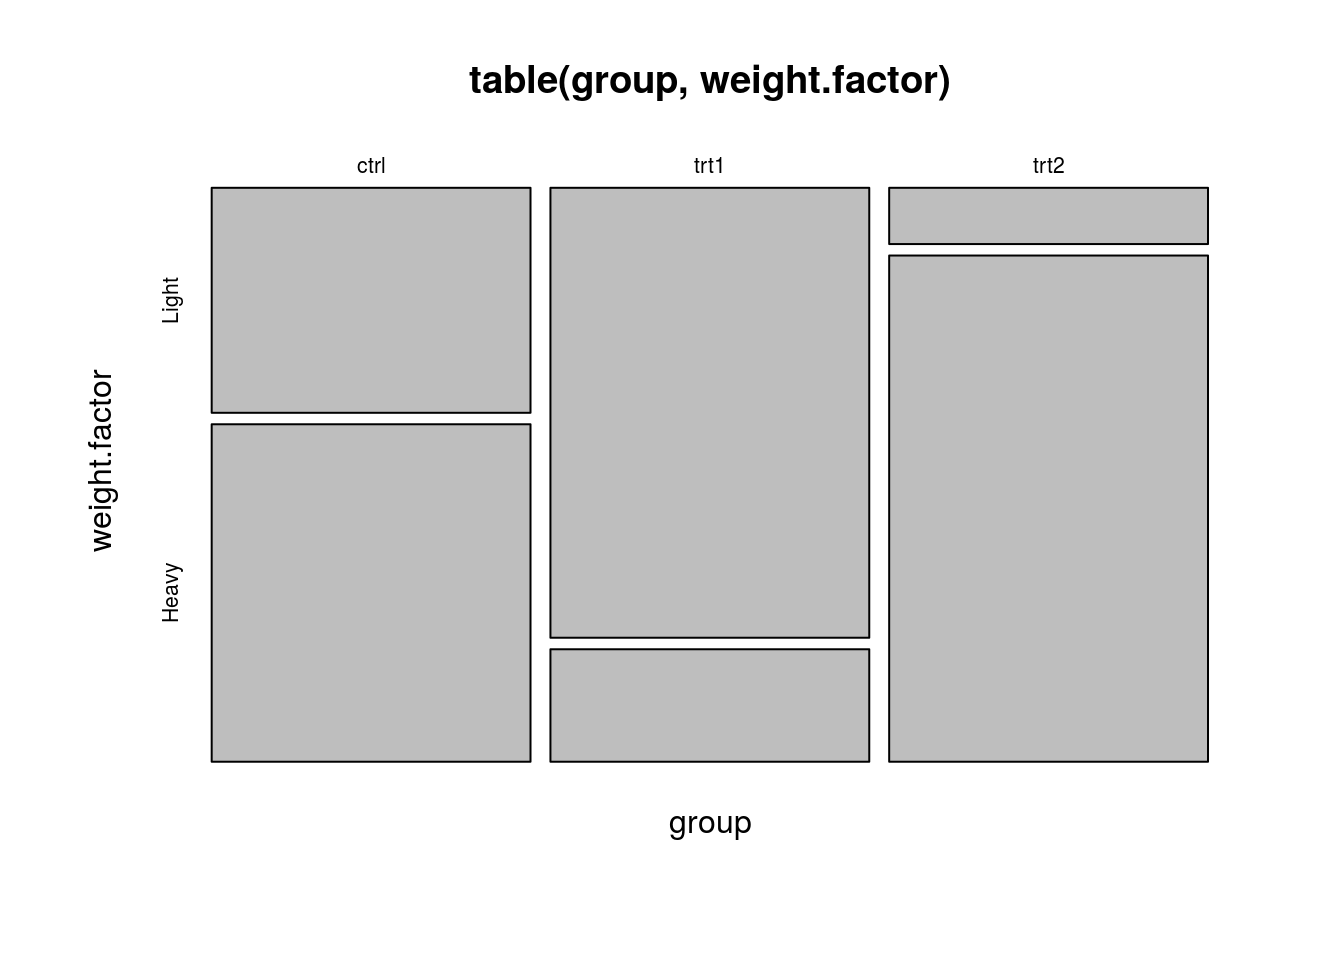
\includegraphics[width=0.5\linewidth]{Rcourse_files/figure-latex/unnamed-chunk-137-1}

Variability in response for each sample type, over the various plates:

\begin{Shaded}
\begin{Highlighting}[]
\KeywordTok{print}\NormalTok{(qrr2[[}\DecValTok{2}\NormalTok{]])  }
\end{Highlighting}
\end{Shaded}

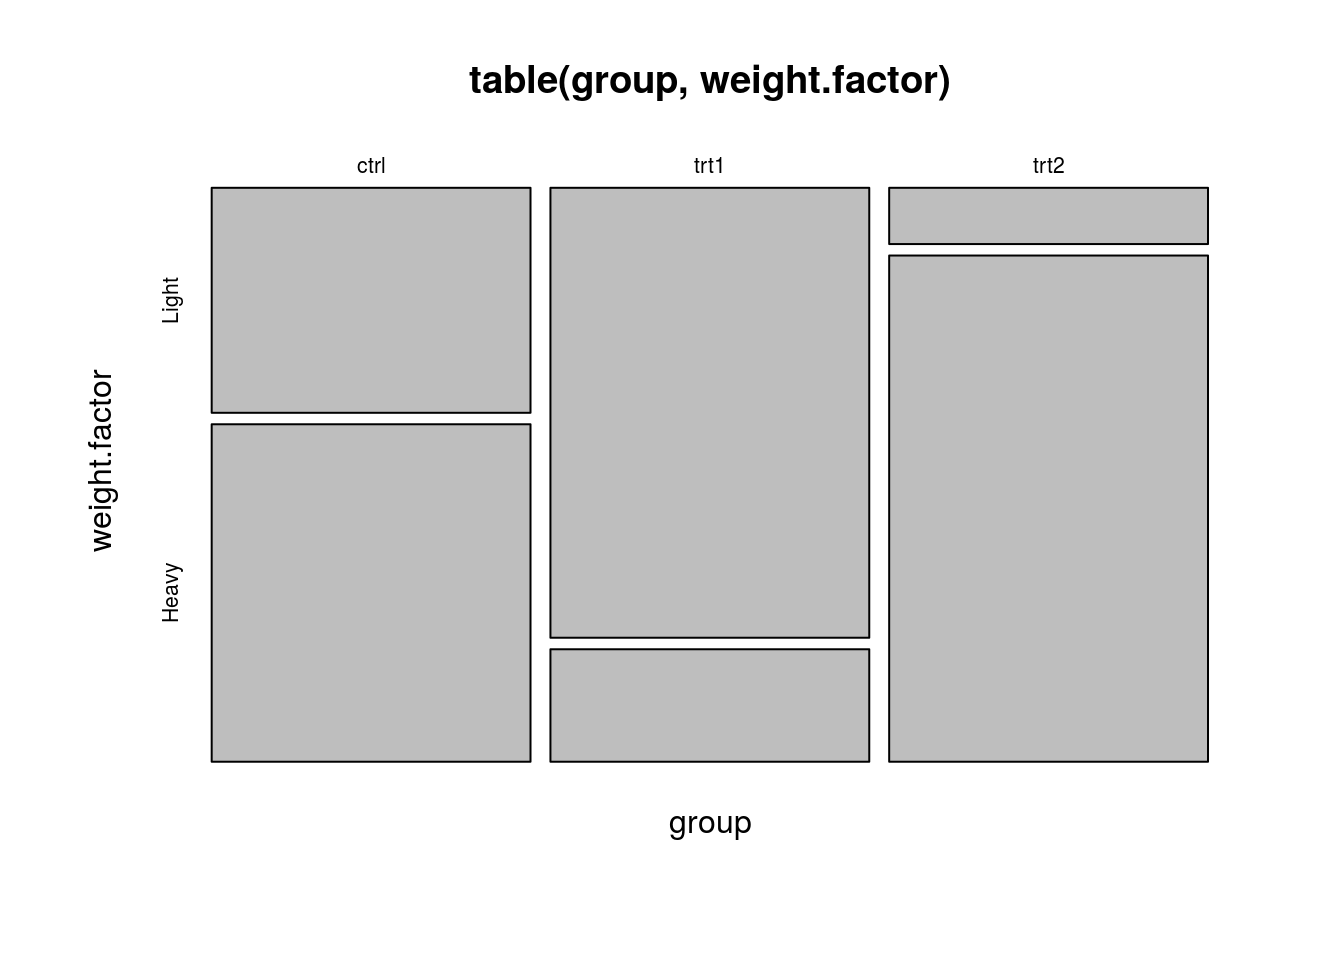
\includegraphics[width=0.5\linewidth]{Rcourse_files/figure-latex/unnamed-chunk-138-1}

\subsection{A Full Mixed-Model}\label{a-full-mixed-model}

In the \texttt{sleepstudy} data, we recorded the reaction times to a
series of tests (\texttt{Reaction}), after various subject
(\texttt{Subject}) underwent various amounts of sleep deprivation
(\texttt{Day}).

\begin{Shaded}
\begin{Highlighting}[]
\KeywordTok{data}\NormalTok{(sleepstudy)}
\NormalTok{lattice::}\KeywordTok{xyplot}\NormalTok{(Reaction ~}\StringTok{ }\NormalTok{Days |}\StringTok{ }\NormalTok{Subject, sleepstudy, }\DataTypeTok{aspect =} \StringTok{"xy"}\NormalTok{,}
             \DataTypeTok{layout =} \KeywordTok{c}\NormalTok{(}\DecValTok{9}\NormalTok{,}\DecValTok{2}\NormalTok{), }\DataTypeTok{type =} \KeywordTok{c}\NormalTok{(}\StringTok{"g"}\NormalTok{, }\StringTok{"p"}\NormalTok{, }\StringTok{"r"}\NormalTok{),}
             \DataTypeTok{index.cond =} \NormalTok{function(x,y) }\KeywordTok{coef}\NormalTok{(}\KeywordTok{lm}\NormalTok{(y ~}\StringTok{ }\NormalTok{x))[}\DecValTok{1}\NormalTok{],}
             \DataTypeTok{xlab =} \StringTok{"Days of sleep deprivation"}\NormalTok{,}
             \DataTypeTok{ylab =} \StringTok{"Average reaction time (ms)"}\NormalTok{)}
\end{Highlighting}
\end{Shaded}

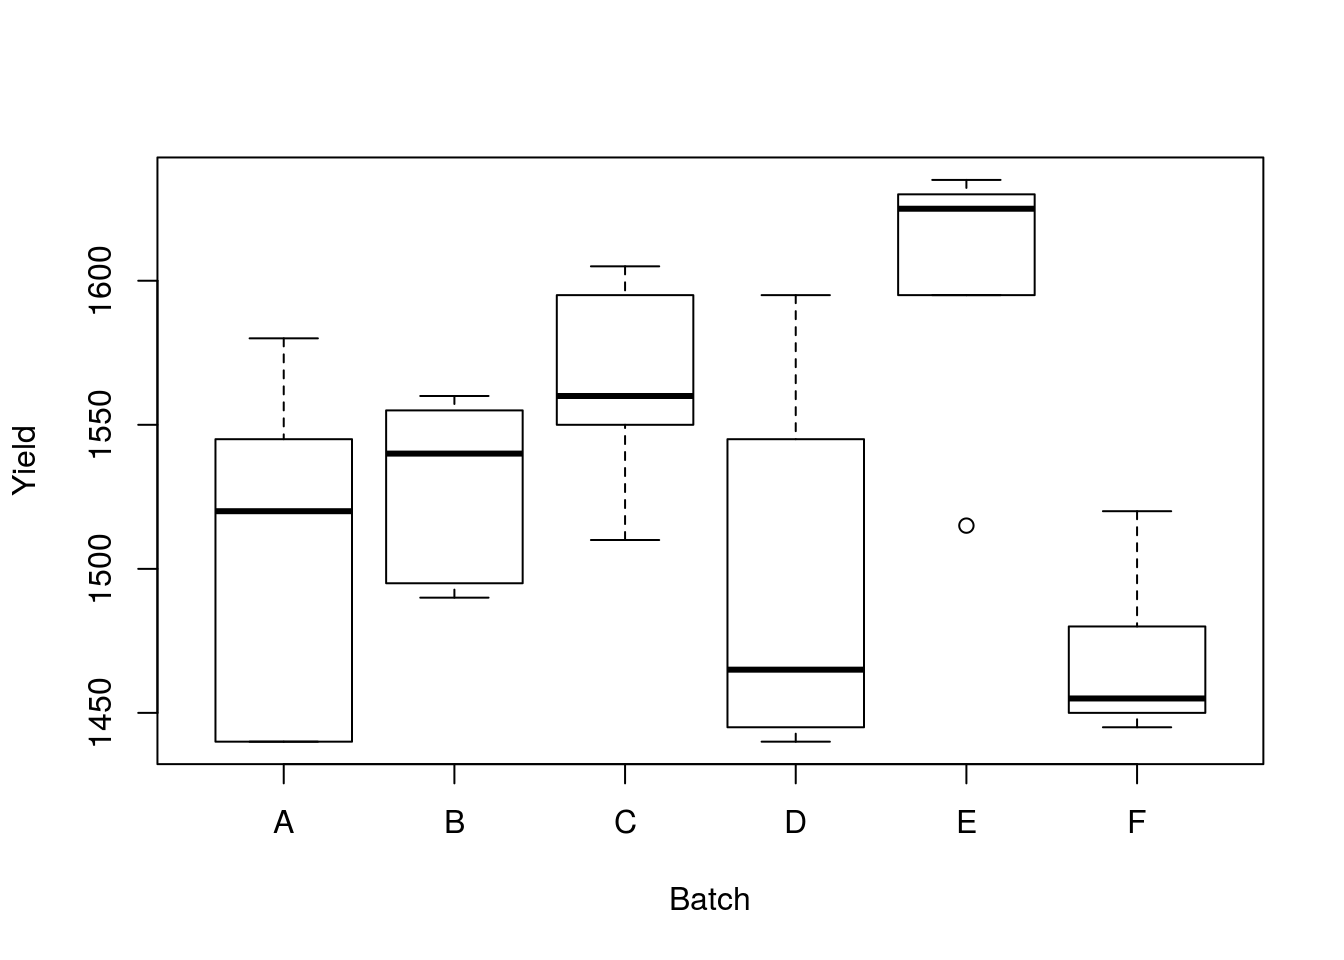
\includegraphics[width=0.5\linewidth]{Rcourse_files/figure-latex/unnamed-chunk-139-1}

We now want to estimate the (fixed) effect of the days of deprivation,
while allowing each subject to have his/hers own effect. The fixed
effect can thus be thought of as the average slope over subjects.

\begin{Shaded}
\begin{Highlighting}[]
\NormalTok{lme}\FloatTok{.3} \NormalTok{<-}\StringTok{ }\KeywordTok{lmer} \NormalTok{( Reaction ~}\StringTok{ }\NormalTok{Days +}\StringTok{ }\NormalTok{( Days |}\StringTok{ }\NormalTok{Subject ) , }\DataTypeTok{data=} \NormalTok{sleepstudy )}
\end{Highlighting}
\end{Shaded}

Things to note:

\begin{itemize}
\tightlist
\item
  We used the \texttt{Days\textbar{}Subect} syntax to tell R we want to
  fit the model \texttt{\textasciitilde{}Days} within each subject.
\item
  Were we fitting the model for purposes of prediction only, an (almost)
  equivalent \texttt{lm}formulation is
  \texttt{lm(Reaction\textasciitilde{}Days*Subject)}.
\end{itemize}

The fixed (i.e.~average) day effect is:

\begin{Shaded}
\begin{Highlighting}[]
\KeywordTok{fixef}\NormalTok{(lme}\FloatTok{.3}\NormalTok{)}
\end{Highlighting}
\end{Shaded}

\begin{verbatim}
## (Intercept)        Days 
##   251.40510    10.46729
\end{verbatim}

The variability in the average response (intercept) and day effect is

\begin{Shaded}
\begin{Highlighting}[]
\KeywordTok{ranef}\NormalTok{(lme}\FloatTok{.3}\NormalTok{)}
\end{Highlighting}
\end{Shaded}

\begin{verbatim}
## $Subject
##     (Intercept)        Days
## 308   2.2585654   9.1989719
## 309 -40.3985770  -8.6197032
## 310 -38.9602459  -5.4488799
## 330  23.6904985  -4.8143313
## 331  22.2602027  -3.0698946
## 332   9.0395259  -0.2721707
## 333  16.8404312  -0.2236244
## 334  -7.2325792   1.0745761
## 335  -0.3336959 -10.7521591
## 337  34.8903509   8.6282839
## 349 -25.2101104   1.1734143
## 350 -13.0699567   6.6142050
## 351   4.5778352  -3.0152572
## 352  20.8635925   3.5360133
## 369   3.2754530   0.8722166
## 370 -25.6128694   4.8224646
## 371   0.8070397  -0.9881551
## 372  12.3145394   1.2840297
\end{verbatim}

Did we really need the whole \texttt{lme} machinery to fit a
within-subject linear regression and then average over subjects? The
answer is yes. The assumptions on the distribution of random effect,
namely, that they are normally distributed, allows us to pool
information from one subject to another. In the words of John Tukey:
``we borrow strength over subjects''. Is this a good thing? If the
normality assumption is true, it certainly is.

To demonstrate the ``strength borrowing'', here is a comparison of the
subject-wise intercepts of the mixed-model, versus a subject-wise linear
model. They are not the same.

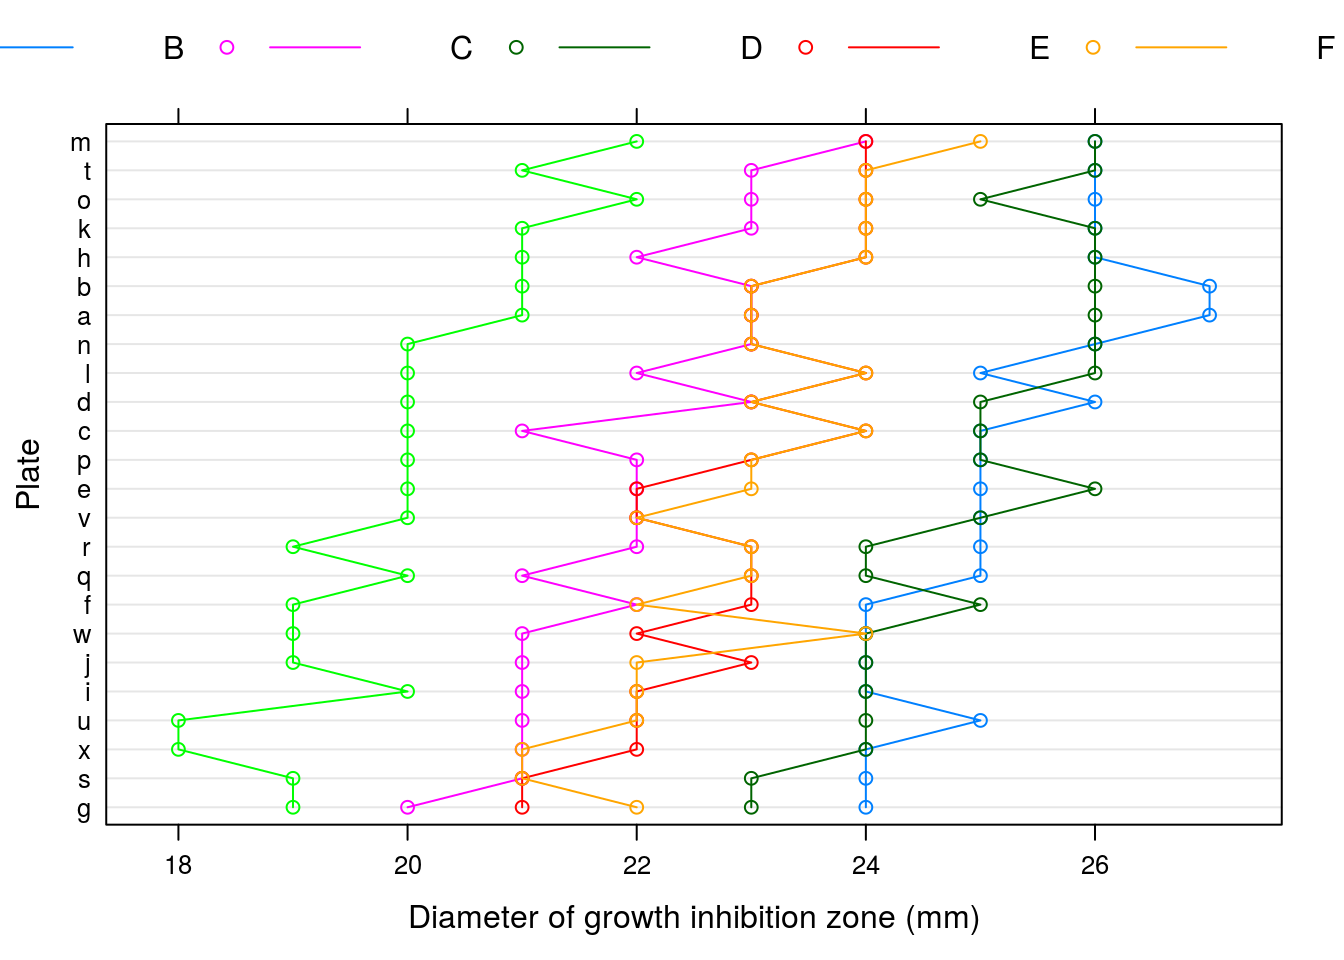
\includegraphics[width=0.5\linewidth]{Rcourse_files/figure-latex/unnamed-chunk-142-1}

Here is a comparison of the random-day effect from \texttt{lme} versus a
subject-wise linear model. They are not the same.

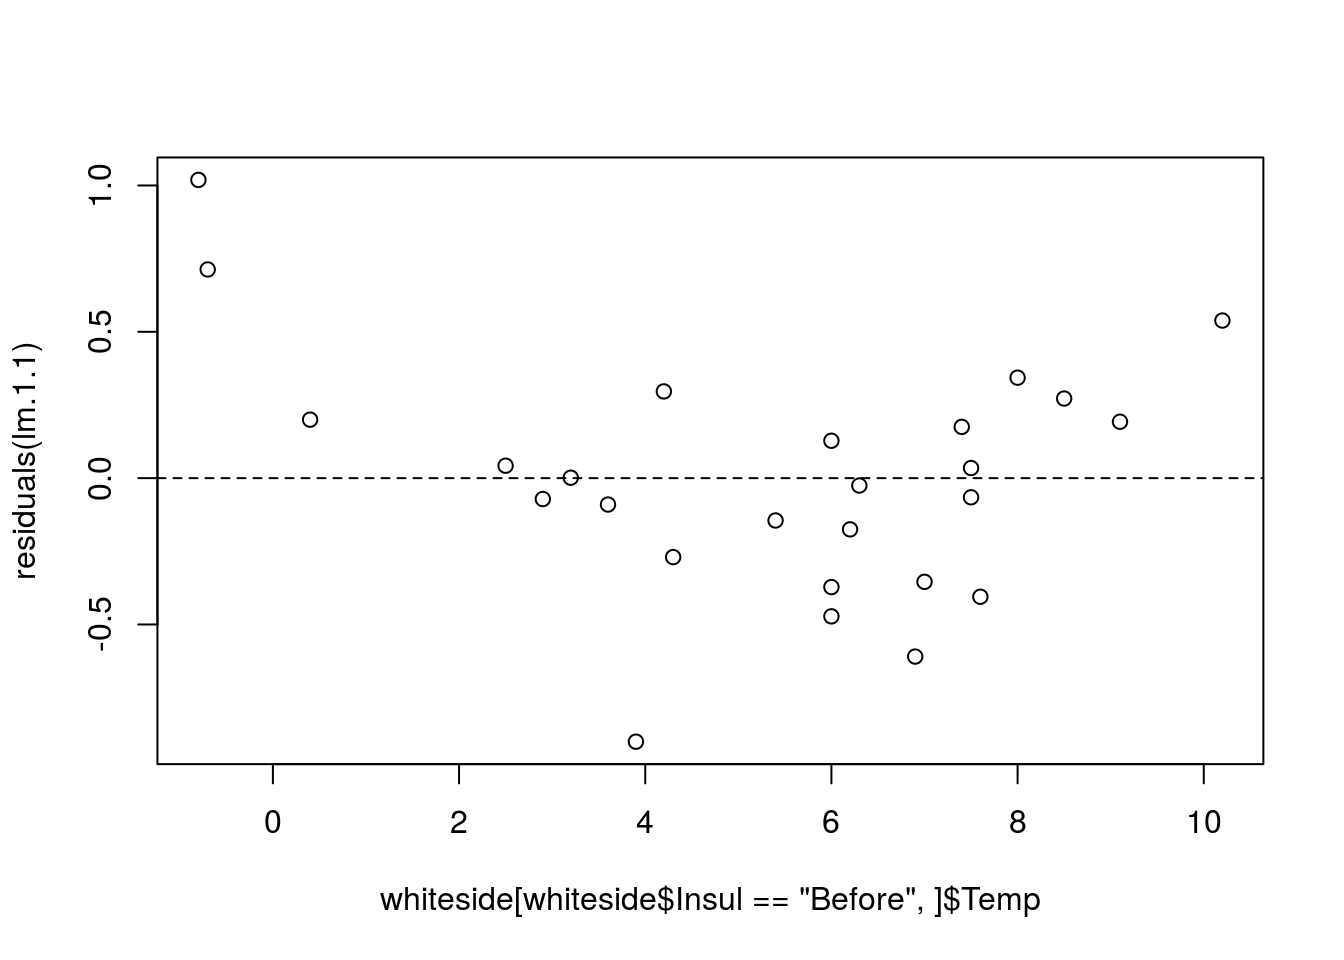
\includegraphics[width=0.5\linewidth]{Rcourse_files/figure-latex/unnamed-chunk-143-1}

\section{Bibliographic Notes}\label{bibliographic-notes-5}

Most of the examples in this chapter are from the documentation of the
\textbf{lme4} package \citep{lme4}. For a more theoretical view see
\citet{weiss2005modeling} or \citet{searle2009variance}. As usual, a
hands on view can be found in \citet{venables2013modern}.

\chapter{Multivariate Data Analysis}\label{multivariate}

The term ``multivariate data analysis'' is so broad and so overloaded,
that we start by clarifying what is discussed and what is not discussed
in this chapter. Broadly speaking, we will discuss statistical
inference, and leave more ``exploratory flavored'' matters like
clustering, and visualization, to the Unsupervised Learning Chapter
\ref{unsupervised}.

More formally, let \(y\) be a \(p\) variate random vector, with
\(E[y]=\mu\). We will discuss the problems of

\begin{itemize}
\tightlist
\item
  \textbf{Signal detection}: a.k.a. \emph{multivariate hypothesis
  testing}, i.e., testing if \(\mu\) equals \(\mu_0\) and for
  \(\mu_0=0\) in particular.
\item
  \textbf{Signal counting}: Counting the number of elements in \(\mu\)
  that differ from \(\mu_0\), and for \(\mu_0=0\) in particular.
\item
  \textbf{Signal identification}: a.k.a. \emph{multiple testing}, i.e.,
  testing which of the elements in \(\mu\) differ from \(\mu_0\) and for
  \(\mu_0=0\) in particular.
\item
  \textbf{Signal estimation}: a.k.a. \emph{selective inference}, i.e.,
  estimating the magnitudes of the departure of \(\mu\) from \(\mu_0\),
  and for \(\mu_0=0\) in particular.
\item
  \textbf{Multivariate Regression}: a.k.a. \emph{MANOVA} in statistical
  literature, and \emph{structured learning} in the machine learning
  literature.
\item
  \textbf{Distribution fitting}: A.k.a. \emph{structure learning} in the
  machine learning literature, deals with the fitting a distribution to
  samples from \(y\). In particular, it deals with the identification of
  independencies between elements of \(y\). For samples from a
  multivariate Gaussian distribution, learning the distribution implies
  all the above problem applied to \(Var[y]\), instead of \(E[y]\).
\end{itemize}

\section{Signal Detection}\label{signal-detection}

\section{Signal Counting}\label{signal-counting}

\section{Signal Identification}\label{signal-identification}

\section{Signal Estimation}\label{signal-estimation}

\section{Multivariate Regression}\label{multivariate-regression}

\section{Distribution Fitting}\label{distribution-fitting}

\chapter{Supervised Learning}\label{supervised}

Machine learning is very similar to statistics, but it is certainly not
the same. As the name suggests, in machine learning we want machines to
learn. This means that we want to replace hard-coded expert algorithm,
with data-driven self-learned algorithm.

There are many learning setups, that depend on what is available to the
machine. The most common setup, discussed in this chapter, is
\emph{supervised learning}. The name takes from the fact that by giving
the machine data samples with known inputs (a.k.a. features) and desired
outputs (a.k.a. labels), the human is effectively supervising the
learning. If we think of the inputs as predictors, and outcomes as
predicted, it is no wonder that supervised learning is very similar to
statistical prediction. When asked ``are these the same?'' I like to
give the example of internet fraud. If you take a sample of fraud
``attacks'', a statistical formulation of the problem is highly
unlikely. This is because fraud events are not randomly drawn from some
distribution, but rather, arrive from an adversary learning the defenses
and adapting to it. This instance of supervised learning belongs in game
theory, more than it does in statistics.

Other types of machine learning problems include:

\begin{itemize}
\tightlist
\item
  \textbf{Unsupervised learning}: See Chapter \ref{unsupervised}.
\item
  \textbf{Semi supervised learning}: Where only part of the samples are
  labeled. A.k.a. \emph{co-training}, \emph{learning from labeled and
  unlabeled data}, \emph{transductive learning}.
\item
  \textbf{Active learning}: Where the machine is allowed to query the
  user for labels. Very similar to \emph{adaptive design of
  experiments}.
\item
  \textbf{Reinforcement learning}: Similar to active learning, in that
  the machine may query for labels. Different from active learning, in
  that the machine does not receive labels, but \emph{rewards}.
\item
  \textbf{Learning on a budget}: A version of active learning where
  querying for labels induces variable costs.
\item
  \textbf{Structure learning}: The learning of the dependence structure
  between variables.
\item
  \textbf{Learning to learn}: Deals with the carriage of ``experience''
  from one learning problem to another. A.k.a. \emph{cummulative
  learning} and \emph{meta learning}.
\item
  \textbf{Manifold learning}: An instance of unsupervised learning,
  where the goal is to reduce the dimension of the data by embedding it
  into a lower dimensional manifold. A.k.a. \emph{support estimation}.
\end{itemize}

\section{Problem setup}\label{problem-setup-3}

We now present the \emph{empirical risk minimization} to supervised
learning.

\BeginKnitrBlock{remark}
\iffalse {Remark. } \fi We do not discuss purely algorithmic approaches
such as K-nearest neighbour and \emph{kernel smoothing} due to space
constraints. For a broader review of supervised learning, see the
Bibliographic Notes section.
\EndKnitrBlock{remark}

Given \(n\) samples with inputs \(x\) from some space \(\mathcal{X}\)
and desired outcome, \(y\), from some space \(\mathcal{Y}\). Samples,
\((x,y)\) have some distribution we denote \(P\). We want to learn a
function that maps inputs to outputs. This function is called a
\emph{hypothesis}, or \emph{predictor}, or \emph{classifier} denoted
\(f\), that belongs to a hypothesis class \(\mathcal{F}\) such that
\(f:\mathcal{X} \to \mathcal{Y}\). We also choose some other function
that fines us for erroneous prediction. This function is called the
\emph{loss}, and we denote it by
\(l:\mathcal{Y}\times \mathcal{Y} \to \mathbb{R}^+\).

\BeginKnitrBlock{remark}
\iffalse {Remark. } \fi The \emph{hypothesis} in machine learning is
only vaguely related the \emph{hypothesis} in statistical testing, which
is quite confusing.
\EndKnitrBlock{remark}

\BeginKnitrBlock{remark}
\iffalse {Remark. } \fi The \emph{hypothesis} in machine learning is not
a bona-fide \emph{statistical model} since we don't assume it is the
data generating process, but rather some function which we choose for
its good predictive performance.
\EndKnitrBlock{remark}

The fundamental task in supervised (statistical) learning is to recover
a hypothesis that minimizes the average loss in the sample, and not in
the population. This is know as the \emph{risk minimization problem}.

\begin{align}
  f^* := argmin_f \{ E_P[l(f(x),y)] \}
  \label{eq:risk}  
\end{align}

To make things more explicit, \(f\) may be a linear function, and \(l\)
a squared error loss, in which case problem \eqref{eq:risk} collapses to

\begin{align}
  f^* := argmin_\beta \{ E_P[(x'\beta-y)^2] \}
\end{align}

Another fundamental problem is that we do not know the distribution of
all possible inputs and outputs, \(P\). We typically only have a sample
of \((x_i,y_i), i=1,\dots,n\). We thus state the \emph{empirical}
counterpart of \eqref{eq:risk}, which consists of minimizing the average
loss. This is known as the \emph{empirical risk miminization} problem
(ERM).

\begin{align}
  \hat f := argmin_f \{ \sum_i l(f(x_i),y_i) \}
  \label{eq:erm}  
\end{align}

Making things more explicit again by using a linear hypothesis with
squared loss, we see that the empirical risk minimization problem
collapses to an ordinary least-squares problem:

\begin{align}
  \hat f := argmin_\beta \{ \sum_i (x_\beta-y_i)^2 \}
\end{align}

When data is samples are independent, then maximum likelihood estimation
is also an instance of ERM, when using the (negative) log likelihood as
the loss function.

If we don't assume any structure on the hypothesis, \(f\), then
\(\hat f\) from \eqref{eq:erm} will interpolate the data, and will be a
very bad predictor. We say, it will \emph{overfit} the observed data,
and will have bad performance on new data.

We have several ways to avoid overfitting:

\begin{enumerate}
\def\labelenumi{\arabic{enumi}.}
\tightlist
\item
  Restrict the hypothesis class \(\mathcal{F}\) (such as linear
  functions).
\item
  Penalize for the complexity of \(f\). The penalty denoted by
  \(\Vert f \Vert\).
\item
  Unbiased risk estimation, where we deal with the overfitted optimism
  of the empirical risk by debiasing it.
\end{enumerate}

\subsection{Common Hypothesis Classes}\label{common-hypothesis-classes}

Some common hypothesis classes, \(\mathcal{F}\), with restricted
complexity, are:

\begin{enumerate}
\def\labelenumi{\arabic{enumi}.}
\tightlist
\item
  \textbf{Linear hypotheses}: such as linear models, GLMs, and (linear)
  support vector machines (SVM).
\item
  \textbf{Neural networks}: a.k.a. \emph{feed-forward} neural nets,
  \emph{artificial} neural nets, and the celebrated class of \emph{deep}
  neural nets.
\item
  \textbf{Tree}: a.k.a. \emph{decision rules}, is a class of hypotheses
  which can be stated as ``if-then'' rules.
\item
  \textbf{Reproducing Kernel Hilbert Space}: a.k.a. RKHS, is a subset of
  ``the space of all functions\footnote{It is even a subset of the
    Hilbert space, itself a subset of the space of all functions.}''
  that is both large enough to capture very complicated relations, but
  small enough so that it is less prone to overfitting, and also
  surprisingly simple to compute with.
\item
  \textbf{Ensembles}: a ``meta'' hypothesis class, which consists of
  taking multiple hypotheses, possibly from different classes, and
  combining them.
\end{enumerate}

\subsection{Common Complexity
Penalties}\label{common-complexity-penalties}

The most common complexity penalty applied to classes that have a finite
dimensional parametric representation, such as a the linear class
parametrized via its coefficients \(\beta\). In such classes we may
penalize for the norm of the parameters. Common penalties include:

\begin{enumerate}
\def\labelenumi{\arabic{enumi}.}
\tightlist
\item
  \textbf{Ridge penalty}: penalizing the \(l_2\) norm of the parameter.
  I.e. \(\Vert f \Vert=\Vert \beta \Vert_2^2=\sum_j \beta_j^2\).
\item
  \textbf{Lasso penalty}: penalizing the \(l_1\) norm of the parameter.
  I.e., \(\Vert f \Vert=\Vert \beta \Vert_1=\sum_j |\beta_j|\)
\item
  \textbf{Elastic net}: a combination of the lasso and ridge penalty.
  I.e.
  ,\(\Vert f \Vert= \alpha \Vert \beta \Vert_2^2 + (a-\alpha) \Vert \beta \Vert_1\).
\end{enumerate}

If the hypothesis class \(\mathcal{F}\) does not admit a finite
dimensional parametric representation, we may penalize it with some
functional norm such as \(\Vert f \Vert_2^2=\int f(t)^2 dt\).

\subsection{Unbiased Risk Estimation}\label{unbiased-risk-estimation}

The fundamental problem of overfitting, is that the empirical risk,
\eqref{eq:erm}, is downward biased to the true risk \eqref{eq:risk}, a.k.a.
\emph{generalization error}, and \emph{test error}. Why is that? Think
of estimating a population's mean with the sample minimum. It can be
done, but the minimum has to be debiased for it to estimate the
population mean. Debiasing methods broadly fall under purely algorithmic
\emph{resampling} based approaches, and theory driven debiasing
corrections. These corrections feel like the penalties above, but we
state them here because unlike the ridge, and lasso, they are designed
for a different purpose.

\begin{enumerate}
\def\labelenumi{\arabic{enumi}.}
\tightlist
\item
  \textbf{Train,Validate,Test}: The simplest form of validation is to
  split the data. A \emph{train} set to train a set of hypotheses. A
  \emph{validation} set to compute the out-of-sample expected loss, and
  pick the best performing hypothesis. A \emph{test} sample to compute
  the out-of-sample performance of the selected hypothesis. This is a
  very simple approach, but it is very ``data inefficient'', thus
  motivating the next method.
\item
  \textbf{V-fold cross validation}: By far the most popular performance
  assessment algorithm, in \emph{V-fold CV} we ``fold'' the data into
  \(V\) non-overlapping sets. For each of the \(V\) sets, we fit a
  hypothesis to the non-selected fold, and assess the expected loss on
  the selected loss. We then aggregate results over the \(V\) folds,
  typically by averaging.
\item
  \textbf{AIC}: Akaike's information criterion (AIC) is a theory driven
  correction of the empirical risk, so that it is unbiased to the true
  risk. It is appropriate when using the likelihood loss.
\item
  \textbf{Cp}: Mallow's Cp is an instance of AIC for likelihood loss
  under normal noise.
\end{enumerate}

Other theory driven unbiased risk estimators include the \emph{Bayesian
Information Criterion} (BIC, aka SBC, aka SBIC), the \emph{Minimum
Description Length} (MDL), \emph{Vapnic's Structural Risk Minimization}
(SRM), the \emph{Deviance Information Criterion} (DIC), and the
\emph{Hannan-Quinn Information Criterion} (HQC).

Other resampling based unbiased risk estimators include resampling
\textbf{without replacement} algorithms like \emph{delete-d cross
validation} with its many variations, and \textbf{resampling with
replacement}, like the \emph{bootstrap}, with its many variations.

\subsection{Collecting the Pieces}\label{collecting-the-pieces}

An ERM problem with regularization will look like

\begin{align}
  \hat f := argmin_f \{ \sum_i l(f(x_i),y_i)  + \lambda \Vert f \Vert \}
  \label{eq:erm-regularized}  
\end{align}

Collecting ideas from the above sections, a typical supervised learning
pipeline will include: choosing the hypothesis class, choosing the
penalty function and level, choosing the assessment algorithm. We
emphasize that choosing the penalty function is not enough, and we need
to choose how ``hard'' to apply it. This if known as the
\emph{regularization level}, typically denoted by \(\lambda\), which
enters

Examples of such combos include:

\begin{enumerate}
\def\labelenumi{\arabic{enumi}.}
\tightlist
\item
  Linear regression, no penalty, train-validate test.
\item
  Linear regression, no penalty, AIC.
\item
  Linear regression, \(l_2\) penalty, V-fold CV. This combo is typically
  known as \emph{ridge regression}.
\item
  Linear regression, \(l_1\) penalty, V-fold CV. This combo is typically
  known as \emph{lasso regression}.
\item
  Linear regression, \(l_1\) and \(l_2\) penalty, V-fold CV. This combo
  is typically known as \emph{elastic net regression}.
\item
  Logistic regression, \(l_2\) penalty, V-fold CV.
\item
  SVM classification, \(l_2\) penalty, V-fold CV.
\item
  Deep network, no penalty, V-fold CV.
\end{enumerate}

For fans of statistical hypothesis testing we will also emphasize:
Testing and prediction are related, but are not the same. \textbf{It is
indeed possible that we will want to ignore a significant predictor, and
add a non-significant one!} \citep{foster2004variable} Some authors will
use hypothesis testing as an initial screening of candidate predictors.
This is a useful heuristic, but that is all it is-- a heuristic.

\section{Supervised Learning in R}\label{supervised-learning-in-r}

At this point, we have a rich enough language to do supervised learning
with R.

In these examples, I will use two data sets from the
\textbf{ElemStatLearn} package: \texttt{spam} for categorical
predictions (spam mail or not spam?), and \texttt{prostate} for
continuous predictions (size of cancerous tumor). In \texttt{spam} we
will try to decide if a mail is spam or not. In \texttt{prostate} we
will try to predict the size of a cancerous tumor. You can now call
\texttt{?prostate} and \texttt{?spam} to learn more about these data
sets.

Some boring pre-processing.

\begin{Shaded}
\begin{Highlighting}[]
\KeywordTok{library}\NormalTok{(ElemStatLearn) }\CommentTok{# for data}
\KeywordTok{data}\NormalTok{(}\StringTok{"prostate"}\NormalTok{)}
\KeywordTok{data}\NormalTok{(}\StringTok{"spam"}\NormalTok{)}

\KeywordTok{library}\NormalTok{(magrittr) }\CommentTok{# for piping}

\CommentTok{# Preparing prostate data}
\NormalTok{prostate.train <-}\StringTok{ }\NormalTok{prostate[prostate$train, }\KeywordTok{names}\NormalTok{(prostate)!=}\StringTok{'train'}\NormalTok{]}
\NormalTok{prostate.test <-}\StringTok{ }\NormalTok{prostate[!prostate$train, }\KeywordTok{names}\NormalTok{(prostate)!=}\StringTok{'train'}\NormalTok{] }
\NormalTok{y.train <-}\StringTok{ }\NormalTok{prostate.train$lcavol}
\NormalTok{X.train <-}\StringTok{ }\KeywordTok{as.matrix}\NormalTok{(prostate.train[, }\KeywordTok{names}\NormalTok{(prostate.train)!=}\StringTok{'lcavol'}\NormalTok{] )}
\NormalTok{y.test <-}\StringTok{ }\NormalTok{prostate.test$lcavol }
\NormalTok{X.test <-}\StringTok{ }\KeywordTok{as.matrix}\NormalTok{(prostate.test[, }\KeywordTok{names}\NormalTok{(prostate.test)!=}\StringTok{'lcavol'}\NormalTok{] )}

\CommentTok{# Preparing spam data:}
\NormalTok{n <-}\StringTok{ }\KeywordTok{nrow}\NormalTok{(spam)}

\NormalTok{train.prop <-}\StringTok{ }\FloatTok{0.66}
\NormalTok{train.ind <-}\StringTok{ }\KeywordTok{c}\NormalTok{(}\OtherTok{TRUE}\NormalTok{,}\OtherTok{FALSE}\NormalTok{) %>%}\StringTok{  }
\StringTok{  }\KeywordTok{sample}\NormalTok{(}\DataTypeTok{size =} \NormalTok{n, }\DataTypeTok{prob =} \KeywordTok{c}\NormalTok{(train.prop,}\DecValTok{1}\NormalTok{-train.prop), }\DataTypeTok{replace=}\OtherTok{TRUE}\NormalTok{)}
\NormalTok{spam.train <-}\StringTok{ }\NormalTok{spam[train.ind,]}
\NormalTok{spam.test <-}\StringTok{ }\NormalTok{spam[!train.ind,]}

\NormalTok{y.train.spam <-}\StringTok{ }\NormalTok{spam.train$spam}
\NormalTok{X.train.spam <-}\StringTok{ }\KeywordTok{as.matrix}\NormalTok{(spam.train[,}\KeywordTok{names}\NormalTok{(spam.train)!=}\StringTok{'spam'}\NormalTok{] )}
\NormalTok{y.test.spam <-}\StringTok{ }\NormalTok{spam.test$spam}
\NormalTok{X.test.spam <-}\StringTok{  }\KeywordTok{as.matrix}\NormalTok{(spam.test[,}\KeywordTok{names}\NormalTok{(spam.test)!=}\StringTok{'spam'}\NormalTok{]) }

\NormalTok{spam.dummy <-}\StringTok{ }\NormalTok{spam}
\NormalTok{spam.dummy$spam <-}\StringTok{ }\KeywordTok{as.numeric}\NormalTok{(spam$spam==}\StringTok{'spam'}\NormalTok{) }
\NormalTok{spam.train.dummy <-}\StringTok{ }\NormalTok{spam.dummy[train.ind,]}
\NormalTok{spam.test.dummy <-}\StringTok{ }\NormalTok{spam.dummy[!train.ind,]}
\end{Highlighting}
\end{Shaded}

We also load some utility functions that we will require down the road.

\begin{Shaded}
\begin{Highlighting}[]
\NormalTok{l2 <-}\StringTok{ }\NormalTok{function(x) x^}\DecValTok{2} \NormalTok\StringTok{ }\NormalTok{sum %>%}\StringTok{ }\NormalTok{sqrt }
\NormalTok{l1 <-}\StringTok{ }\NormalTok{function(x) }\KeywordTok{abs}\NormalTok{(x) %>%}\StringTok{ }\NormalTok{sum  }
\NormalTok{MSE <-}\StringTok{ }\NormalTok{function(x) x^}\DecValTok{2} \NormalTok\StringTok{ }\NormalTok{mean }
\NormalTok{missclassification <-}\StringTok{ }\NormalTok{function(tab) }\KeywordTok{sum}\NormalTok{(tab[}\KeywordTok{c}\NormalTok{(}\DecValTok{2}\NormalTok{,}\DecValTok{3}\NormalTok{)])/}\KeywordTok{sum}\NormalTok{(tab)}
\end{Highlighting}
\end{Shaded}

\subsection{Linear Models with Least Squares Loss}\label{least-squares}

Starting with OLS regression, and a train-test data approach. Notice the
better in-sample MSE than the out-of-sample. That is overfitting in
action.

\begin{Shaded}
\begin{Highlighting}[]
\NormalTok{ols}\FloatTok{.1} \NormalTok{<-}\StringTok{ }\KeywordTok{lm}\NormalTok{(lcavol~. ,}\DataTypeTok{data =} \NormalTok{prostate.train)}
\CommentTok{# Train error:}
\KeywordTok{MSE}\NormalTok{( }\KeywordTok{predict}\NormalTok{(ols}\FloatTok{.1}\NormalTok{)-}\StringTok{ }\NormalTok{prostate.train$lcavol) }
\end{Highlighting}
\end{Shaded}

\begin{verbatim}
## [1] 0.4383709
\end{verbatim}

\begin{Shaded}
\begin{Highlighting}[]
\CommentTok{# Test error:}
\KeywordTok{MSE}\NormalTok{( }\KeywordTok{predict}\NormalTok{(ols}\FloatTok{.1}\NormalTok{, }\DataTypeTok{newdata =} \NormalTok{prostate.test)-}\StringTok{ }\NormalTok{prostate.test$lcavol)}
\end{Highlighting}
\end{Shaded}

\begin{verbatim}
## [1] 0.5084068
\end{verbatim}

We now implement a V-fold CV, instead of our train-test approach. The
assignment of each observation to each fold is encoded in
\texttt{fold.assignment}. The following implementation is extremely
inefficient, but easy to read.

\begin{Shaded}
\begin{Highlighting}[]
\NormalTok{folds <-}\StringTok{ }\DecValTok{10}
\NormalTok{fold.assignment <-}\StringTok{ }\KeywordTok{sample}\NormalTok{(}\DecValTok{1}\NormalTok{:}\DecValTok{5}\NormalTok{, }\KeywordTok{nrow}\NormalTok{(prostate), }\DataTypeTok{replace =} \OtherTok{TRUE}\NormalTok{)}
\NormalTok{errors <-}\StringTok{ }\OtherTok{NULL}

\NormalTok{for (k in }\DecValTok{1}\NormalTok{:folds)\{}
  \NormalTok{prostate.cross.train <-}\StringTok{ }\NormalTok{prostate[fold.assignment!=k,] }\CommentTok{# train subset}
  \NormalTok{prostate.cross.test <-}\StringTok{  }\NormalTok{prostate[fold.assignment==k,] }\CommentTok{# test subset}
  \NormalTok{.ols <-}\StringTok{ }\KeywordTok{lm}\NormalTok{(lcavol~. ,}\DataTypeTok{data =} \NormalTok{prostate.cross.train) }\CommentTok{# train}
  \NormalTok{.predictions <-}\StringTok{ }\KeywordTok{predict}\NormalTok{(.ols, }\DataTypeTok{newdata=}\NormalTok{prostate.cross.test)}
  \NormalTok{.errors <-}\StringTok{  }\NormalTok{.predictions -}\StringTok{ }\NormalTok{prostate.cross.test$lcavol }\CommentTok{# save prediction errors in the fold}
  \NormalTok{errors <-}\StringTok{ }\KeywordTok{c}\NormalTok{(errors, .errors) }\CommentTok{# aggregate error over folds.}
\NormalTok{\}}

\CommentTok{# Cross validated prediction error:}
\KeywordTok{MSE}\NormalTok{(errors)}
\end{Highlighting}
\end{Shaded}

\begin{verbatim}
## [1] 0.6024089
\end{verbatim}

Let's try all possible models, and choose the best performer with
respect to the Cp criterion. We see that the best performer has 3
predictors.

\begin{Shaded}
\begin{Highlighting}[]
\KeywordTok{library}\NormalTok{(leaps)}
\NormalTok{regfit.full <-}\StringTok{ }\NormalTok{prostate.train %>%}\StringTok{ }
\StringTok{  }\KeywordTok{regsubsets}\NormalTok{(lcavol~.,}\DataTypeTok{data =} \NormalTok{., }\DataTypeTok{method =} \StringTok{'exhaustive'}\NormalTok{) }\CommentTok{# best subset selection}
\KeywordTok{plot}\NormalTok{(regfit.full, }\DataTypeTok{scale =} \StringTok{"Cp"}\NormalTok{)}
\end{Highlighting}
\end{Shaded}

\includegraphics[width=0.5\linewidth]{Rcourse_files/figure-latex/all subset-1}

Instead of the Cp criterion, we now compute the train and test errors
for all the possible predictors\footnote{Example taken from
  \url{https://lagunita.stanford.edu/c4x/HumanitiesScience/StatLearning/asset/ch6.html}}.

\begin{Shaded}
\begin{Highlighting}[]
\NormalTok{model.n <-}\StringTok{ }\NormalTok{regfit.full %>%}\StringTok{ }\NormalTok{summary %>%}\StringTok{ }\NormalTok{length}
\NormalTok{X.train.named <-}\StringTok{ }\NormalTok{prostate.train %>%}\StringTok{ }\KeywordTok{model.matrix}\NormalTok{(lcavol ~}\StringTok{ }\NormalTok{., }\DataTypeTok{data =} \NormalTok{.)}
\NormalTok{X.train.named <-}\StringTok{ }\KeywordTok{model.matrix}\NormalTok{(lcavol ~}\StringTok{ }\NormalTok{., }\DataTypeTok{data =} \NormalTok{prostate.train ) }
\NormalTok{X.test.named <-}\StringTok{ }\KeywordTok{model.matrix}\NormalTok{(lcavol ~}\StringTok{ }\NormalTok{., }\DataTypeTok{data =} \NormalTok{prostate.test ) }


\NormalTok{val.errors <-}\StringTok{ }\KeywordTok{rep}\NormalTok{(}\OtherTok{NA}\NormalTok{, model.n)}
\NormalTok{train.errors <-}\StringTok{ }\KeywordTok{rep}\NormalTok{(}\OtherTok{NA}\NormalTok{, model.n)}
\NormalTok{for (i in }\DecValTok{1}\NormalTok{:model.n) \{}
    \NormalTok{coefi <-}\StringTok{ }\KeywordTok{coef}\NormalTok{(regfit.full, }\DataTypeTok{id =} \NormalTok{i)}
    
    \NormalTok{pred <-}\StringTok{  }\NormalTok{X.train.named[, }\KeywordTok{names}\NormalTok{(coefi)] %*%}\StringTok{ }\NormalTok{coefi}
    \NormalTok{train.errors[i] <-}\StringTok{ }\KeywordTok{MSE}\NormalTok{(y.train -}\StringTok{ }\NormalTok{pred)}

    \NormalTok{pred <-}\StringTok{  }\NormalTok{X.test.named[, }\KeywordTok{names}\NormalTok{(coefi)] %*%}\StringTok{ }\NormalTok{coefi}
    \NormalTok{val.errors[i] <-}\StringTok{ }\KeywordTok{MSE}\NormalTok{(y.test -}\StringTok{ }\NormalTok{pred)}
\NormalTok{\}}
\KeywordTok{plot}\NormalTok{(train.errors, }\DataTypeTok{ylab =} \StringTok{"MSE"}\NormalTok{, }\DataTypeTok{pch =} \DecValTok{19}\NormalTok{, }\DataTypeTok{type =} \StringTok{"o"}\NormalTok{)}
\KeywordTok{points}\NormalTok{(val.errors, }\DataTypeTok{pch =} \DecValTok{19}\NormalTok{, }\DataTypeTok{type =} \StringTok{"b"}\NormalTok{, }\DataTypeTok{col=}\StringTok{"blue"}\NormalTok{)}
\KeywordTok{legend}\NormalTok{(}\StringTok{"topright"}\NormalTok{, }
       \DataTypeTok{legend =} \KeywordTok{c}\NormalTok{(}\StringTok{"Training"}\NormalTok{, }\StringTok{"Validation"}\NormalTok{), }
       \DataTypeTok{col =} \KeywordTok{c}\NormalTok{(}\StringTok{"black"}\NormalTok{, }\StringTok{"blue"}\NormalTok{), }
       \DataTypeTok{pch =} \DecValTok{19}\NormalTok{)}
\end{Highlighting}
\end{Shaded}

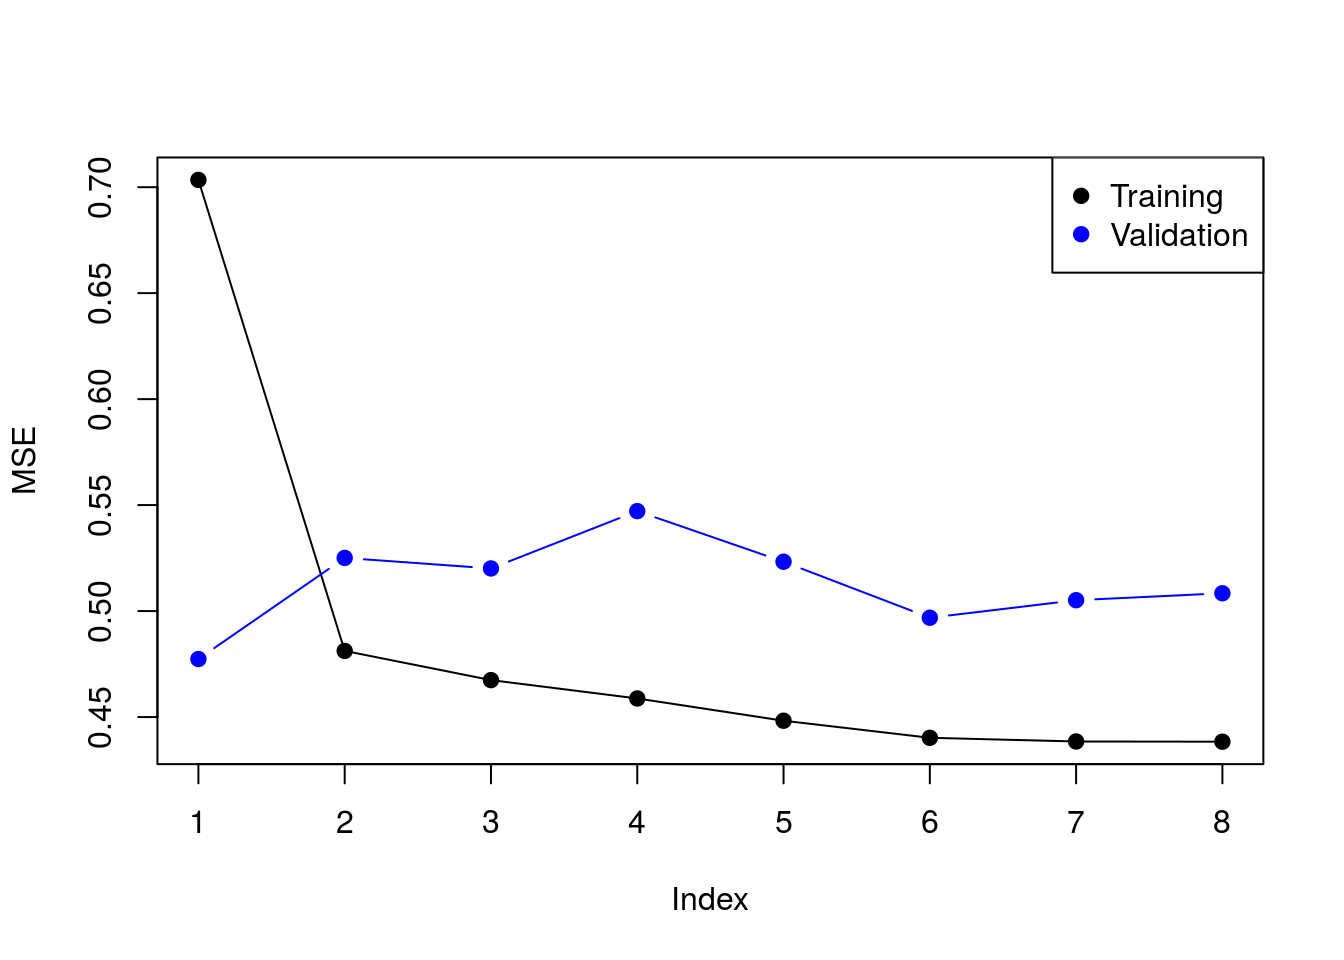
\includegraphics[width=0.5\linewidth]{Rcourse_files/figure-latex/unnamed-chunk-148-1}

Checking all possible models is computationally very hard. \emph{Forward
selection} is a greedy approach that adds one variable at a time, using
the AIC criterion. If AIC falls, the variable is added.

\begin{Shaded}
\begin{Highlighting}[]
\NormalTok{ols}\FloatTok{.0} \NormalTok{<-}\StringTok{ }\KeywordTok{lm}\NormalTok{(lcavol~}\DecValTok{1} \NormalTok{,}\DataTypeTok{data =} \NormalTok{prostate.train)}
\NormalTok{model.scope <-}\StringTok{ }\KeywordTok{list}\NormalTok{(}\DataTypeTok{upper=}\NormalTok{ols}\FloatTok{.1}\NormalTok{, }\DataTypeTok{lower=}\NormalTok{ols}\FloatTok{.0}\NormalTok{)}
\KeywordTok{step}\NormalTok{(ols}\FloatTok{.0}\NormalTok{, }\DataTypeTok{scope=}\NormalTok{model.scope, }\DataTypeTok{direction=}\StringTok{'forward'}\NormalTok{, }\DataTypeTok{trace =} \OtherTok{TRUE}\NormalTok{)}
\end{Highlighting}
\end{Shaded}

\begin{verbatim}
## Start:  AIC=30.1
## lcavol ~ 1
## 
##           Df Sum of Sq     RSS     AIC
## + lpsa     1    54.776  47.130 -19.570
## + lcp      1    48.805  53.101 -11.578
## + svi      1    35.829  66.077   3.071
## + pgg45    1    23.789  78.117  14.285
## + gleason  1    18.529  83.377  18.651
## + lweight  1     9.186  92.720  25.768
## + age      1     8.354  93.552  26.366
## <none>                 101.906  30.097
## + lbph     1     0.407 101.499  31.829
## 
## Step:  AIC=-19.57
## lcavol ~ lpsa
## 
##           Df Sum of Sq    RSS     AIC
## + lcp      1   14.8895 32.240 -43.009
## + svi      1    5.0373 42.093 -25.143
## + gleason  1    3.5500 43.580 -22.817
## + pgg45    1    3.0503 44.080 -22.053
## + lbph     1    1.8389 45.291 -20.236
## + age      1    1.5329 45.597 -19.785
## <none>                 47.130 -19.570
## + lweight  1    0.4106 46.719 -18.156
## 
## Step:  AIC=-43.01
## lcavol ~ lpsa + lcp
## 
##           Df Sum of Sq    RSS     AIC
## <none>                 32.240 -43.009
## + age      1   0.92315 31.317 -42.955
## + pgg45    1   0.29594 31.944 -41.627
## + gleason  1   0.21500 32.025 -41.457
## + lbph     1   0.13904 32.101 -41.298
## + lweight  1   0.05504 32.185 -41.123
## + svi      1   0.02069 32.220 -41.052
\end{verbatim}

\begin{verbatim}
## 
## Call:
## lm(formula = lcavol ~ lpsa + lcp, data = prostate.train)
## 
## Coefficients:
## (Intercept)         lpsa          lcp  
##     0.08798      0.53369      0.38879
\end{verbatim}

We now learn a linear predictor on the \texttt{spam} data using, with
least squares loss, and train-test validation.

\begin{Shaded}
\begin{Highlighting}[]
\CommentTok{# train the predictor}
\NormalTok{ols}\FloatTok{.2} \NormalTok{<-}\StringTok{ }\KeywordTok{lm}\NormalTok{(spam~., }\DataTypeTok{data =} \NormalTok{spam.train.dummy) }

\CommentTok{# make in-sample predictions}
\NormalTok{.predictions.train <-}\StringTok{ }\KeywordTok{predict}\NormalTok{(ols}\FloatTok{.2}\NormalTok{) >}\StringTok{ }\FloatTok{0.5} 
\CommentTok{# inspect the confusion matrix}
\NormalTok{(confusion.train <-}\StringTok{ }\KeywordTok{table}\NormalTok{(}\DataTypeTok{prediction=}\NormalTok{.predictions.train, }\DataTypeTok{truth=}\NormalTok{spam.train.dummy$spam)) }
\end{Highlighting}
\end{Shaded}

\begin{verbatim}
##           truth
## prediction    0    1
##      FALSE 1748  234
##      TRUE    84  956
\end{verbatim}

\begin{Shaded}
\begin{Highlighting}[]
\CommentTok{# compute the train (in sample) misclassification}
\KeywordTok{missclassification}\NormalTok{(confusion.train) }
\end{Highlighting}
\end{Shaded}

\begin{verbatim}
## [1] 0.1052283
\end{verbatim}

\begin{Shaded}
\begin{Highlighting}[]
\CommentTok{# make out-of-sample prediction}
\NormalTok{.predictions.test <-}\StringTok{ }\KeywordTok{predict}\NormalTok{(ols}\FloatTok{.2}\NormalTok{, }\DataTypeTok{newdata =} \NormalTok{spam.test.dummy) >}\StringTok{ }\FloatTok{0.5} 
\CommentTok{# inspect the confusion matrix}
\NormalTok{(confusion.test <-}\StringTok{ }\KeywordTok{table}\NormalTok{(}\DataTypeTok{prediction=}\NormalTok{.predictions.test, }\DataTypeTok{truth=}\NormalTok{spam.test.dummy$spam))}
\end{Highlighting}
\end{Shaded}

\begin{verbatim}
##           truth
## prediction   0   1
##      FALSE 917 129
##      TRUE   39 494
\end{verbatim}

\begin{Shaded}
\begin{Highlighting}[]
\CommentTok{# compute the train (in sample) misclassification}
\KeywordTok{missclassification}\NormalTok{(confusion.test)}
\end{Highlighting}
\end{Shaded}

\begin{verbatim}
## [1] 0.1063965
\end{verbatim}

The \texttt{glmnet} package is an excellent package that provides ridge,
lasso, and elastic net regularization, for all GLMs, so for linear
models in particular.

\begin{Shaded}
\begin{Highlighting}[]
\KeywordTok{suppressMessages}\NormalTok{(}\KeywordTok{library}\NormalTok{(glmnet))}
\NormalTok{ridge}\FloatTok{.2} \NormalTok{<-}\StringTok{ }\KeywordTok{glmnet}\NormalTok{(}\DataTypeTok{x=}\NormalTok{X.train, }\DataTypeTok{y=}\NormalTok{y.train, }\DataTypeTok{family =} \StringTok{'gaussian'}\NormalTok{, }\DataTypeTok{alpha =} \DecValTok{0}\NormalTok{)}

\CommentTok{# Train error:}
\KeywordTok{MSE}\NormalTok{( }\KeywordTok{predict}\NormalTok{(ridge}\FloatTok{.2}\NormalTok{, }\DataTypeTok{newx =}\NormalTok{X.train)-}\StringTok{ }\NormalTok{y.train)}
\end{Highlighting}
\end{Shaded}

\begin{verbatim}
## [1] 1.006028
\end{verbatim}

\begin{Shaded}
\begin{Highlighting}[]
\CommentTok{# Test error:}
\KeywordTok{MSE}\NormalTok{( }\KeywordTok{predict}\NormalTok{(ridge}\FloatTok{.2}\NormalTok{, }\DataTypeTok{newx =} \NormalTok{X.test)-}\StringTok{ }\NormalTok{y.test)}
\end{Highlighting}
\end{Shaded}

\begin{verbatim}
## [1] 0.7678264
\end{verbatim}

Things to note:

\begin{itemize}
\tightlist
\item
  The \texttt{alpha=0} parameters tells R to do ridge regression.
  Setting \(alpha=1\) will do lasso, and any other value, with return an
  elastic net with appropriate weights.
\item
  The `family=`gaussian' argument tells R to fit a linear model, with
  least squares loss.
\end{itemize}

We now use the lasso penalty.

\begin{Shaded}
\begin{Highlighting}[]
\NormalTok{lasso}\FloatTok{.1} \NormalTok{<-}\StringTok{ }\KeywordTok{glmnet}\NormalTok{(}\DataTypeTok{x=}\NormalTok{X.train, }\DataTypeTok{y=}\NormalTok{y.train, , }\DataTypeTok{family=}\StringTok{'gaussian'}\NormalTok{, }\DataTypeTok{alpha =} \DecValTok{1}\NormalTok{)}

\CommentTok{# Train error:}
\KeywordTok{MSE}\NormalTok{( }\KeywordTok{predict}\NormalTok{(lasso}\FloatTok{.1}\NormalTok{, }\DataTypeTok{newx =}\NormalTok{X.train)-}\StringTok{ }\NormalTok{y.train)}
\end{Highlighting}
\end{Shaded}

\begin{verbatim}
## [1] 0.5525279
\end{verbatim}

\begin{Shaded}
\begin{Highlighting}[]
\CommentTok{# Test error:}
\KeywordTok{MSE}\NormalTok{( }\KeywordTok{predict}\NormalTok{(lasso}\FloatTok{.1}\NormalTok{, }\DataTypeTok{newx =} \NormalTok{X.test)-}\StringTok{ }\NormalTok{y.test)}
\end{Highlighting}
\end{Shaded}

\begin{verbatim}
## [1] 0.5211263
\end{verbatim}

We now use \texttt{glmnet} for classification.

\begin{Shaded}
\begin{Highlighting}[]
\NormalTok{logistic}\FloatTok{.2} \NormalTok{<-}\StringTok{ }\KeywordTok{cv.glmnet}\NormalTok{(}\DataTypeTok{x=}\NormalTok{X.train.spam, }\DataTypeTok{y=}\NormalTok{y.train.spam, }\DataTypeTok{family =} \StringTok{"binomial"}\NormalTok{, }\DataTypeTok{alpha =} \DecValTok{0}\NormalTok{)}
\end{Highlighting}
\end{Shaded}

Things to note:

\begin{itemize}
\tightlist
\item
  We used \texttt{cv.glmnet} to do an automatic search for the optimal
  level of regularization (the \texttt{lambda} argument in
  \texttt{glmnet}).
\item
  We set \texttt{alpha=0} for ridge regression.
\end{itemize}

\begin{Shaded}
\begin{Highlighting}[]
\CommentTok{# Train confusion matrix:}
\NormalTok{.predictions.train <-}\StringTok{ }\KeywordTok{predict}\NormalTok{(logistic}\FloatTok{.2}\NormalTok{, }\DataTypeTok{newx =} \NormalTok{X.train.spam, }\DataTypeTok{type =} \StringTok{'class'}\NormalTok{) }
\NormalTok{(confusion.train <-}\StringTok{ }\KeywordTok{table}\NormalTok{(}\DataTypeTok{prediction=}\NormalTok{.predictions.train, }\DataTypeTok{truth=}\NormalTok{spam.train$spam))}
\end{Highlighting}
\end{Shaded}

\begin{verbatim}
##           truth
## prediction email spam
##      email  1753  178
##      spam     79 1012
\end{verbatim}

\begin{Shaded}
\begin{Highlighting}[]
\CommentTok{# Train misclassification error}
\KeywordTok{missclassification}\NormalTok{(confusion.train)}
\end{Highlighting}
\end{Shaded}

\begin{verbatim}
## [1] 0.08504302
\end{verbatim}

\begin{Shaded}
\begin{Highlighting}[]
\CommentTok{# Test confusion matrix:}
\NormalTok{.predictions.test <-}\StringTok{ }\KeywordTok{predict}\NormalTok{(logistic}\FloatTok{.2}\NormalTok{, }\DataTypeTok{newx =} \NormalTok{X.test.spam, }\DataTypeTok{type=}\StringTok{'class'}\NormalTok{) }
\NormalTok{(confusion.test <-}\StringTok{ }\KeywordTok{table}\NormalTok{(}\DataTypeTok{prediction=}\NormalTok{.predictions.test, }\DataTypeTok{truth=}\NormalTok{y.test.spam))}
\end{Highlighting}
\end{Shaded}

\begin{verbatim}
##           truth
## prediction email spam
##      email   915   93
##      spam     41  530
\end{verbatim}

\begin{Shaded}
\begin{Highlighting}[]
\CommentTok{# Test misclassification error:}
\KeywordTok{missclassification}\NormalTok{(confusion.test)}
\end{Highlighting}
\end{Shaded}

\begin{verbatim}
## [1] 0.08486384
\end{verbatim}

\subsection{SVM}\label{svm}

A support vector machine (SVM) is a linear model with a particular loss
function known as a \emph{hinge loss}. We learn an SVM with the
\texttt{svm} function from the \textbf{e1071} package, which is merely a
wrapper for the \textbf{libsvm} C library, which is the most popular
implementation of SVM today.

\begin{Shaded}
\begin{Highlighting}[]
\KeywordTok{library}\NormalTok{(e1071)}
\NormalTok{svm}\FloatTok{.1} \NormalTok{<-}\StringTok{ }\KeywordTok{svm}\NormalTok{(spam~., }\DataTypeTok{data =} \NormalTok{spam.train)}

\CommentTok{# Train confusion matrix:}
\NormalTok{.predictions.train <-}\StringTok{ }\KeywordTok{predict}\NormalTok{(svm}\FloatTok{.1}\NormalTok{) }
\NormalTok{(confusion.train <-}\StringTok{ }\KeywordTok{table}\NormalTok{(}\DataTypeTok{prediction=}\NormalTok{.predictions.train, }\DataTypeTok{truth=}\NormalTok{spam.train$spam))}
\end{Highlighting}
\end{Shaded}

\begin{verbatim}
##           truth
## prediction email spam
##      email  1775   98
##      spam     57 1092
\end{verbatim}

\begin{Shaded}
\begin{Highlighting}[]
\KeywordTok{missclassification}\NormalTok{(confusion.train)}
\end{Highlighting}
\end{Shaded}

\begin{verbatim}
## [1] 0.05129054
\end{verbatim}

\begin{Shaded}
\begin{Highlighting}[]
\CommentTok{# Test confusion matrix:}
\NormalTok{.predictions.test <-}\StringTok{ }\KeywordTok{predict}\NormalTok{(svm}\FloatTok{.1}\NormalTok{, }\DataTypeTok{newdata =} \NormalTok{spam.test) }
\NormalTok{(confusion.test <-}\StringTok{ }\KeywordTok{table}\NormalTok{(}\DataTypeTok{prediction=}\NormalTok{.predictions.test, }\DataTypeTok{truth=}\NormalTok{spam.test$spam))}
\end{Highlighting}
\end{Shaded}

\begin{verbatim}
##           truth
## prediction email spam
##      email   920   77
##      spam     36  546
\end{verbatim}

\begin{Shaded}
\begin{Highlighting}[]
\KeywordTok{missclassification}\NormalTok{(confusion.test)}
\end{Highlighting}
\end{Shaded}

\begin{verbatim}
## [1] 0.07156428
\end{verbatim}

We can also use SVM for regression.

\begin{Shaded}
\begin{Highlighting}[]
\NormalTok{svm}\FloatTok{.2} \NormalTok{<-}\StringTok{ }\KeywordTok{svm}\NormalTok{(lcavol~., }\DataTypeTok{data =} \NormalTok{prostate.train)}

\CommentTok{# Train error:}
\KeywordTok{MSE}\NormalTok{( }\KeywordTok{predict}\NormalTok{(svm}\FloatTok{.2}\NormalTok{)-}\StringTok{ }\NormalTok{prostate.train$lcavol)}
\end{Highlighting}
\end{Shaded}

\begin{verbatim}
## [1] 0.3336868
\end{verbatim}

\begin{Shaded}
\begin{Highlighting}[]
\CommentTok{# Test error:}
\KeywordTok{MSE}\NormalTok{( }\KeywordTok{predict}\NormalTok{(svm}\FloatTok{.2}\NormalTok{, }\DataTypeTok{newdata =} \NormalTok{prostate.test)-}\StringTok{ }\NormalTok{prostate.test$lcavol)}
\end{Highlighting}
\end{Shaded}

\begin{verbatim}
## [1] 0.5633183
\end{verbatim}

\subsection{Neural Nets}\label{neural-nets}

Neural nets (non deep) can be fitted, for example, with the
\texttt{nnet} function in the \textbf{nnet} package. We start with a
nnet regression.

\begin{Shaded}
\begin{Highlighting}[]
\KeywordTok{library}\NormalTok{(nnet)}
\NormalTok{nnet}\FloatTok{.1} \NormalTok{<-}\StringTok{ }\KeywordTok{nnet}\NormalTok{(lcavol~., }\DataTypeTok{size=}\DecValTok{20}\NormalTok{, }\DataTypeTok{data=}\NormalTok{prostate.train, }\DataTypeTok{rang =} \FloatTok{0.1}\NormalTok{, }\DataTypeTok{decay =} \FloatTok{5e-4}\NormalTok{, }\DataTypeTok{maxit =} \DecValTok{1000}\NormalTok{, }\DataTypeTok{trace=}\OtherTok{FALSE}\NormalTok{)}

\CommentTok{# Train error:}
\KeywordTok{MSE}\NormalTok{( }\KeywordTok{predict}\NormalTok{(nnet}\FloatTok{.1}\NormalTok{)-}\StringTok{ }\NormalTok{prostate.train$lcavol)}
\end{Highlighting}
\end{Shaded}

\begin{verbatim}
## [1] 1.174269
\end{verbatim}

\begin{Shaded}
\begin{Highlighting}[]
\CommentTok{# Test error:}
\KeywordTok{MSE}\NormalTok{( }\KeywordTok{predict}\NormalTok{(nnet}\FloatTok{.1}\NormalTok{, }\DataTypeTok{newdata =} \NormalTok{prostate.test)-}\StringTok{ }\NormalTok{prostate.test$lcavol)}
\end{Highlighting}
\end{Shaded}

\begin{verbatim}
## [1] 1.476749
\end{verbatim}

And nnet classification.

\begin{Shaded}
\begin{Highlighting}[]
\NormalTok{nnet}\FloatTok{.2} \NormalTok{<-}\StringTok{ }\KeywordTok{nnet}\NormalTok{(spam~., }\DataTypeTok{size=}\DecValTok{5}\NormalTok{, }\DataTypeTok{data=}\NormalTok{spam.train, }\DataTypeTok{rang =} \FloatTok{0.1}\NormalTok{, }\DataTypeTok{decay =} \FloatTok{5e-4}\NormalTok{, }\DataTypeTok{maxit =} \DecValTok{1000}\NormalTok{, }\DataTypeTok{trace=}\OtherTok{FALSE}\NormalTok{)}

\CommentTok{# Train confusion matrix:}
\NormalTok{.predictions.train <-}\StringTok{ }\KeywordTok{predict}\NormalTok{(nnet}\FloatTok{.2}\NormalTok{, }\DataTypeTok{type=}\StringTok{'class'}\NormalTok{) }
\NormalTok{(confusion.train <-}\StringTok{ }\KeywordTok{table}\NormalTok{(}\DataTypeTok{prediction=}\NormalTok{.predictions.train, }\DataTypeTok{truth=}\NormalTok{spam.train$spam))}
\end{Highlighting}
\end{Shaded}

\begin{verbatim}
##           truth
## prediction email spam
##      email  1779   59
##      spam     53 1131
\end{verbatim}

\begin{Shaded}
\begin{Highlighting}[]
\KeywordTok{missclassification}\NormalTok{(confusion.train)}
\end{Highlighting}
\end{Shaded}

\begin{verbatim}
## [1] 0.03706155
\end{verbatim}

\begin{Shaded}
\begin{Highlighting}[]
\CommentTok{# Test confusion matrix:}
\NormalTok{.predictions.test <-}\StringTok{ }\KeywordTok{predict}\NormalTok{(nnet}\FloatTok{.2}\NormalTok{, }\DataTypeTok{newdata =} \NormalTok{spam.test, }\DataTypeTok{type=}\StringTok{'class'}\NormalTok{) }
\NormalTok{(confusion.test <-}\StringTok{ }\KeywordTok{table}\NormalTok{(}\DataTypeTok{prediction=}\NormalTok{.predictions.test, }\DataTypeTok{truth=}\NormalTok{spam.test$spam))}
\end{Highlighting}
\end{Shaded}

\begin{verbatim}
##           truth
## prediction email spam
##      email   915   58
##      spam     41  565
\end{verbatim}

\begin{Shaded}
\begin{Highlighting}[]
\KeywordTok{missclassification}\NormalTok{(confusion.test)}
\end{Highlighting}
\end{Shaded}

\begin{verbatim}
## [1] 0.06269791
\end{verbatim}

\subsection{Classification and Regression Trees
(CART)}\label{classification-and-regression-trees-cart}

A CART, is not a linear model. It partitions the feature space
\(\mathcal{X}\), thus creating a set of if-then rules for prediction or
classification. This view clarifies the name of the function
\texttt{rpart}, which \emph{recursively partitions} the feature space.

We start with a regression tree.

\begin{Shaded}
\begin{Highlighting}[]
\KeywordTok{library}\NormalTok{(rpart)}
\NormalTok{tree}\FloatTok{.1} \NormalTok{<-}\StringTok{ }\KeywordTok{rpart}\NormalTok{(lcavol~., }\DataTypeTok{data=}\NormalTok{prostate.train)}

\CommentTok{# Train error:}
\KeywordTok{MSE}\NormalTok{( }\KeywordTok{predict}\NormalTok{(tree}\FloatTok{.1}\NormalTok{)-}\StringTok{ }\NormalTok{prostate.train$lcavol)}
\end{Highlighting}
\end{Shaded}

\begin{verbatim}
## [1] 0.4909568
\end{verbatim}

\begin{Shaded}
\begin{Highlighting}[]
\CommentTok{# Test error:}
\KeywordTok{MSE}\NormalTok{( }\KeywordTok{predict}\NormalTok{(tree}\FloatTok{.1}\NormalTok{, }\DataTypeTok{newdata =} \NormalTok{prostate.test)-}\StringTok{ }\NormalTok{prostate.test$lcavol)}
\end{Highlighting}
\end{Shaded}

\begin{verbatim}
## [1] 0.5623316
\end{verbatim}

Tree are very prone to overfitting. To avoid this, we reduce a tree's
complexity by \emph{pruning} it. This is done with the \texttt{prune}
function.

We now fit a classification tree.

\begin{Shaded}
\begin{Highlighting}[]
\NormalTok{tree}\FloatTok{.2} \NormalTok{<-}\StringTok{ }\KeywordTok{rpart}\NormalTok{(spam~., }\DataTypeTok{data=}\NormalTok{spam.train)}

\CommentTok{# Train confusion matrix:}
\NormalTok{.predictions.train <-}\StringTok{ }\KeywordTok{predict}\NormalTok{(tree}\FloatTok{.2}\NormalTok{, }\DataTypeTok{type=}\StringTok{'class'}\NormalTok{) }
\NormalTok{(confusion.train <-}\StringTok{ }\KeywordTok{table}\NormalTok{(}\DataTypeTok{prediction=}\NormalTok{.predictions.train, }\DataTypeTok{truth=}\NormalTok{spam.train$spam))}
\end{Highlighting}
\end{Shaded}

\begin{verbatim}
##           truth
## prediction email spam
##      email  1755  216
##      spam     77  974
\end{verbatim}

\begin{Shaded}
\begin{Highlighting}[]
\KeywordTok{missclassification}\NormalTok{(confusion.train)}
\end{Highlighting}
\end{Shaded}

\begin{verbatim}
## [1] 0.09695566
\end{verbatim}

\begin{Shaded}
\begin{Highlighting}[]
\CommentTok{# Test confusion matrix:}
\NormalTok{.predictions.test <-}\StringTok{ }\KeywordTok{predict}\NormalTok{(tree}\FloatTok{.2}\NormalTok{, }\DataTypeTok{newdata =} \NormalTok{spam.test, }\DataTypeTok{type=}\StringTok{'class'}\NormalTok{) }
\NormalTok{(confusion.test <-}\StringTok{ }\KeywordTok{table}\NormalTok{(}\DataTypeTok{prediction=}\NormalTok{.predictions.test, }\DataTypeTok{truth=}\NormalTok{spam.test$spam))}
\end{Highlighting}
\end{Shaded}

\begin{verbatim}
##           truth
## prediction email spam
##      email   909  137
##      spam     47  486
\end{verbatim}

\begin{Shaded}
\begin{Highlighting}[]
\KeywordTok{missclassification}\NormalTok{(confusion.test)}
\end{Highlighting}
\end{Shaded}

\begin{verbatim}
## [1] 0.1165294
\end{verbatim}

\subsection{K-nearest neighbour (KNN)}\label{k-nearest-neighbour-knn}

KNN is not an ERM problem. For completeness, we still show how to fit
such a hypothesis.

\begin{Shaded}
\begin{Highlighting}[]
\KeywordTok{library}\NormalTok{(class)}
\NormalTok{knn}\FloatTok{.1} \NormalTok{<-}\StringTok{ }\KeywordTok{knn}\NormalTok{(}\DataTypeTok{train =} \NormalTok{X.train.spam, }\DataTypeTok{test =} \NormalTok{X.test.spam, }\DataTypeTok{cl =}\NormalTok{y.train.spam, }\DataTypeTok{k =} \DecValTok{1}\NormalTok{)}

\CommentTok{# Test confusion matrix:}
\NormalTok{.predictions.test <-}\StringTok{ }\NormalTok{knn}\FloatTok{.1} 
\NormalTok{(confusion.test <-}\StringTok{ }\KeywordTok{table}\NormalTok{(}\DataTypeTok{prediction=}\NormalTok{.predictions.test, }\DataTypeTok{truth=}\NormalTok{spam.test$spam))}
\end{Highlighting}
\end{Shaded}

\begin{verbatim}
##           truth
## prediction email spam
##      email   814  153
##      spam    142  470
\end{verbatim}

\begin{Shaded}
\begin{Highlighting}[]
\KeywordTok{missclassification}\NormalTok{(confusion.test)}
\end{Highlighting}
\end{Shaded}

\begin{verbatim}
## [1] 0.1868271
\end{verbatim}

\subsection{Linear Discriminant Analysis
(LDA)}\label{linear-discriminant-analysis-lda}

LDA is equivalent to least squares classification \ref{least-squares}.
There are, however, some dedicated functions to fit it.

\begin{Shaded}
\begin{Highlighting}[]
\KeywordTok{library}\NormalTok{(MASS) }
\NormalTok{lda}\FloatTok{.1} \NormalTok{<-}\StringTok{ }\KeywordTok{lda}\NormalTok{(spam~., spam.train)}

\CommentTok{# Train confusion matrix:}
\NormalTok{.predictions.train <-}\StringTok{ }\KeywordTok{predict}\NormalTok{(lda}\FloatTok{.1}\NormalTok{)$class}
\NormalTok{(confusion.train <-}\StringTok{ }\KeywordTok{table}\NormalTok{(}\DataTypeTok{prediction=}\NormalTok{.predictions.train, }\DataTypeTok{truth=}\NormalTok{spam.train$spam))}
\end{Highlighting}
\end{Shaded}

\begin{verbatim}
##           truth
## prediction email spam
##      email  1748  234
##      spam     84  956
\end{verbatim}

\begin{Shaded}
\begin{Highlighting}[]
\KeywordTok{missclassification}\NormalTok{(confusion.train)}
\end{Highlighting}
\end{Shaded}

\begin{verbatim}
## [1] 0.1052283
\end{verbatim}

\begin{Shaded}
\begin{Highlighting}[]
\CommentTok{# Test confusion matrix:}
\NormalTok{.predictions.test <-}\StringTok{ }\KeywordTok{predict}\NormalTok{(lda}\FloatTok{.1}\NormalTok{, }\DataTypeTok{newdata =} \NormalTok{spam.test)$class}
\NormalTok{(confusion.test <-}\StringTok{ }\KeywordTok{table}\NormalTok{(}\DataTypeTok{prediction=}\NormalTok{.predictions.test, }\DataTypeTok{truth=}\NormalTok{spam.test$spam))}
\end{Highlighting}
\end{Shaded}

\begin{verbatim}
##           truth
## prediction email spam
##      email   917  125
##      spam     39  498
\end{verbatim}

\begin{Shaded}
\begin{Highlighting}[]
\KeywordTok{missclassification}\NormalTok{(confusion.test)}
\end{Highlighting}
\end{Shaded}

\begin{verbatim}
## [1] 0.1038632
\end{verbatim}

\subsection{Naive Bayes}\label{naive-bayes}

A Naive-Bayes classifier is also not part of the ERM framework. It is,
however, very popular, so we present it.

\begin{Shaded}
\begin{Highlighting}[]
\KeywordTok{library}\NormalTok{(e1071)}
\NormalTok{nb}\FloatTok{.1} \NormalTok{<-}\StringTok{ }\KeywordTok{naiveBayes}\NormalTok{(spam~., }\DataTypeTok{data =} \NormalTok{spam.train)}

\CommentTok{# Train confusion matrix:}
\NormalTok{.predictions.train <-}\StringTok{ }\KeywordTok{predict}\NormalTok{(nb}\FloatTok{.1}\NormalTok{, }\DataTypeTok{newdata =} \NormalTok{spam.train)}
\NormalTok{(confusion.train <-}\StringTok{ }\KeywordTok{table}\NormalTok{(}\DataTypeTok{prediction=}\NormalTok{.predictions.train, }\DataTypeTok{truth=}\NormalTok{spam.train$spam))}
\end{Highlighting}
\end{Shaded}

\begin{verbatim}
##           truth
## prediction email spam
##      email  1068   74
##      spam    764 1116
\end{verbatim}

\begin{Shaded}
\begin{Highlighting}[]
\KeywordTok{missclassification}\NormalTok{(confusion.train)}
\end{Highlighting}
\end{Shaded}

\begin{verbatim}
## [1] 0.2772998
\end{verbatim}

\begin{Shaded}
\begin{Highlighting}[]
\CommentTok{# Test confusion matrix:}
\NormalTok{.predictions.test <-}\StringTok{ }\KeywordTok{predict}\NormalTok{(nb}\FloatTok{.1}\NormalTok{, }\DataTypeTok{newdata =} \NormalTok{spam.test)}
\NormalTok{(confusion.test <-}\StringTok{ }\KeywordTok{table}\NormalTok{(}\DataTypeTok{prediction=}\NormalTok{.predictions.test, }\DataTypeTok{truth=}\NormalTok{spam.test$spam))}
\end{Highlighting}
\end{Shaded}

\begin{verbatim}
##           truth
## prediction email spam
##      email   548   27
##      spam    408  596
\end{verbatim}

\begin{Shaded}
\begin{Highlighting}[]
\KeywordTok{missclassification}\NormalTok{(confusion.test)}
\end{Highlighting}
\end{Shaded}

\begin{verbatim}
## [1] 0.2754908
\end{verbatim}

\section{Bibliographic Notes}\label{bibliographic-notes-6}

The ultimate reference on (statistical) machine learning is
\citet{friedman2001elements}. For a softer introduction, see
\citet{james2013introduction}. A statistician will also like
\citet{ripley2007pattern}. For an R oriented view see
\citet{lantz2013machine}. For a very algorithmic view, see the seminal
\citet{leskovec2014mining} or \citet{conway2012machine}. For a much more
theoretical reference, see \citet{mohri2012foundations},
\citet{vapnik2013nature}, \citet{shalev2014understanding}. Terminology
taken from \citet{sammut2011encyclopedia}. For a review of resampling
based unbiased risk estimation (i.e.~cross validation) see the
exceptional review of \citet{arlot2010survey}.

\chapter{Unsupervised Learning}\label{unsupervised}

This chapter deals with machine learning problems which are
unsupervised. This means the machine has access to a set of inputs,
\(x\), but the desired outcome, \(y\) is not available. Clearly,
learning a relation between inputs and outcomes is impossible, but there
are still a lot of problems of interest. In particular, we may want to
find a compact representation of the inputs, be it for visualization of
further processing. This is the problem of \emph{dimensionality
reduction}. For the same reasons we may want to group similar inputs.
This is the problem of \emph{clustering}.

In the statistical terminology, and with some exceptions, this chapter
can be thought of as multivariate \textbf{exploratory} statistics. For
multivariate \textbf{inference}, see Chapter \ref{multivariate}.

\section{Dimensionality Reduction}\label{dim-reduce}

\BeginKnitrBlock{example}
\protect\hypertarget{ex:bmi}{}{\label{ex:bmi}}Consider the heights and
weights of a sample of individuals. The data may seemingly reside in
\(2\) dimensions but given the height, we have a pretty good guess of a
persons weight, and vice versa. We can thus state that heights and
weights are not really two dimensional, but roughly lay on a \(1\)
dimensional subspace of \(\mathbb{R}^2\).
\EndKnitrBlock{example}

\BeginKnitrBlock{example}
\protect\hypertarget{ex:iq}{}{\label{ex:iq}}Consider the correctness of the
answers to a questionnaire with \(p\) questions. The data may seemingly
reside in a \(p\) dimensional space, but assuming there is a thing as
``skill'', then given the correctness of a person's reply to a subset of
questions, we have a good idea how he scores on the rest. Put
differently, we don't really need a \(200\) question questionnaire--
\(100\) is more than enough. If skill is indeed a one dimensional
quality, then the questionnaire data should organize around a single
line in the \(p\) dimensional cube.
\EndKnitrBlock{example}

\BeginKnitrBlock{example}
\protect\hypertarget{ex:blind-signal}{}{\label{ex:blind-signal}}Consider
\(n\) microphones recording an individual. The digitized recording
consists of \(p\) samples. Are the recordings really a shapeless cloud
of \(n\) points in \(\mathbb{R}^p\)? Since they all record the same
sound, one would expect the \(n\) \(p\)-dimensional points to arrange
around the source sound bit: a point in \(\mathbb{R}^p\). If microphones
have different distances to the source, volumes may differ. We would
thus expect the \(n\) points to arrange about a line that ends at the
source.
\EndKnitrBlock{example}

\subsection{Principal Component Analysis}\label{pca}

\emph{Principal Component Analysis} (PCA) is such a basic technique, it
has been rediscovered and renamed independently in many fields. It can
be found under the names of Discrete Karhunen--Loève Transform;
Hotteling Transform; Proper Orthogonal Decomposition; Eckart--Young
Theorem; Schmidt--Mirsky Theorem; Empirical Orthogonal Functions;
Empirical Eigenfunction Decomposition; Empirical Component Analysis;
Quasi-Harmonic Modes; Spectral Decomposition; Empirical Modal Analysis,
and possibly more\footnote{\url{http://en.wikipedia.org/wiki/Principal_component_analysis}}.
The many names are quite interesting as they offer an insight into the
different problems that led to PCA's (re)discovery.

Return to the BMI problem in Example \ref{ex:bmi}. Assume you wish to
give each individual a ``size score'', that is a \textbf{linear}
combination of height and weight: PCA does just that. It returns the
linear combination that has the largest variability, i.e., the
combination which best distinguishes between individuals.

The variance maximizing motivation above was the one that guided
\citet{hotelling1933analysis}. But \(30\) years before him,
\citet{pearson1901liii} derived the same procedure with a different
motivation in mind. Pearson was also trying to give each individual a
score. He did not care about variance maximization, however. He simply
wanted a small set of coordinates in some (linear) space that
approximates the original data well. Before we proceed, we give an
example to fix ideas. Consider the crime rate data in
\texttt{USArrests}, which encodes reported murder events, assaults,
rapes, and the urban population of each american state.

\begin{Shaded}
\begin{Highlighting}[]
\KeywordTok{head}\NormalTok{(USArrests)}
\end{Highlighting}
\end{Shaded}

\begin{verbatim}
##            Murder Assault UrbanPop Rape
## Alabama      13.2     236       58 21.2
## Alaska       10.0     263       48 44.5
## Arizona       8.1     294       80 31.0
## Arkansas      8.8     190       50 19.5
## California    9.0     276       91 40.6
## Colorado      7.9     204       78 38.7
\end{verbatim}

Following Hotelling's motivation, we may want to given each state a
``crimilality score''. PCA returns the sequence of \(1,\dots,4\) scores
that best separate between states.

\begin{Shaded}
\begin{Highlighting}[]
\NormalTok{USArrests}\FloatTok{.1} \NormalTok{<-}\StringTok{ }\NormalTok{USArrests[,-}\DecValTok{3}\NormalTok{] %>%}\StringTok{ }\NormalTok{scale }\CommentTok{# note the scaling, which is required by some}
\NormalTok{pca}\FloatTok{.1} \NormalTok{<-}\StringTok{ }\KeywordTok{prcomp}\NormalTok{(USArrests}\FloatTok{.1}\NormalTok{, }\DataTypeTok{scale =} \OtherTok{TRUE}\NormalTok{)}
\NormalTok{pca}\FloatTok{.1}
\end{Highlighting}
\end{Shaded}

\begin{verbatim}
## Standard deviations:
## [1] 1.5357670 0.6767949 0.4282154
## 
## Rotation:
##                PC1        PC2        PC3
## Murder  -0.5826006  0.5339532 -0.6127565
## Assault -0.6079818  0.2140236  0.7645600
## Rape    -0.5393836 -0.8179779 -0.1999436
\end{verbatim}

Things to note:

\begin{itemize}
\tightlist
\item
  Distinguishing between states, i.e., finding the variance maximizing
  scores, should be indifferent to the \textbf{average} of each
  variable. We also don't want the score to be sensitive to the
  measurement \textbf{scale}. We thus perform PCA in the z-score scale
  of each variable, obtained with the \texttt{scale} function.
\item
  PCA is performed with the \texttt{prcomp} function. It returns the
  contribution (weight) of the original variables, to the new crimeness
  score.\\
  These weights are called the \emph{loadings}.
\item
  The number of possible scores, is the same as the number of original
  variables in the data.
\item
  The new scores are called the \emph{principal components}, labeled
  \texttt{PC1},\ldots{},\texttt{PC4} in our output.
\item
  The loadings on PC1 tell us that the best separation between states is
  along the average crime rate. Why is this? Because all the \(3\) crime
  variables have a similar loading on PC1.
\item
  The other PCs are slightly harder to interpret, but it is an
  interesting exercise.
\end{itemize}

\textbf{If we now represent each state, not with its original \(4\)
variables, but only with the first \(2\) PCs (for example), we have
reduced the dimensionality of the data.}

\subsection{Preliminaries}\label{preliminaries}

Before presenting methods other than PCA, we need some terminology.

\begin{itemize}
\tightlist
\item
  \textbf{Variable}: A.k.a. \emph{dimension}, or \emph{feature}, or
  \emph{column} for reasons that will be obvious in the next item.
\item
  \textbf{Data}: A.k.a. \emph{sample}, \emph{observations}. Will
  typically consist of \(n\), \(p\) dimensional vectors. We typically
  denote the data as a \(n\times p\) matrix \(X\).
\item
  \textbf{Manifold}: A generalization of a linear space, which is
  regular enough so that, \textbf{locally}, it has all the properties of
  a linear space. We will denote an arbitrary manifold by
  \(\mathcal{M}\), and by \(\mathcal{M}_q\) a \(q\)
  dimensional\footnote{You are probably used to thinking of the
    \textbf{dimension} of linear spaces. We will not rigorously define
    what is the dimension of a manifold, but you may think of it as the
    number of free coordinates needed to navigate along the manifold.}
  manifold.
\item
  \textbf{Embedding}: Informally speaking: a ``shape preserving''
  mapping of a space into another.
\item
  \textbf{Linear Embedding}: An embedding done via a linear operation
  (thus representable by a matrix).
\item
  \textbf{Generative Model}: Known to statisticians as the
  \textbf{sampling distribution}. The assumed stochastic process that
  generated the observed \(X\).
\end{itemize}

There are many motivations for dimensionality reduction:

\begin{enumerate}
\def\labelenumi{\arabic{enumi}.}
\tightlist
\item
  \textbf{Scoring}: Give each observation an interpretable, simple score
  (Hotelling's motivation).
\item
  \textbf{Latent structure}: Recover unobservables from indirect
  measurements. E.g: Blind signal reconstruction, CT scan, cryo-electron
  microscopy, etc.
\item
  \textbf{Signal to Noise}: Denoise measurements before further
  processing like clustering, supervised learning, etc.
\item
  \textbf{Compression}: Save on RAM ,CPU, and communication when
  operating on a lower dimensional representation of the data.
\end{enumerate}

\subsection{Latent Variable
Approaches}\label{latent-variable-approaches}

All generative approaches to dimensionality reduction will include some
unobserved set of variables, which we can try to recover from the
observable \(X\). The unobservable variables will typically have a lower
dimension than the observables, thus, dimension is reduced. We start
with the simplest case of linear Factor Analysis.

\subsubsection{Factor Analysis (FA)}\label{factor-analysis-fa}

FA originates from the psychometric literature. We thus revisit the IQ
(actually g-factor\footnote{\url{https://en.wikipedia.org/wiki/G_factor_(psychometrics)}})
Example\textasciitilde{}\ref{ex:iq}:

\BeginKnitrBlock{example}
\protect\hypertarget{ex:unnamed-chunk-156}{}{\label{ex:unnamed-chunk-156}}Assume
\(n\) respondents answer \(p\) quantitative questions:
\(x_i \in \mathbb{R}^p, i=1,\dots,n\). Also assume, their responses are
some linear function \(A \in \mathbb{R}^p\) of a single personality
attribute, \(s_i\). We can think of \(s_i\) as the subject's
``intelligence''. We thus have

\begin{align}
    x_i = A s_i + \varepsilon_i
\end{align}

And in matrix notation, for \(q<p\) latent attributes:

\begin{align}
    X = S A+\varepsilon,
    \label{eq:factor}
\end{align}

where \(A\) is the \(q \times p\) matrix of factor loadings, and \(S\)
the \(n \times q\) matrix of latent personality traits. In our
particular example where \(q=1\), the problem is to recover the
unobservable intelligence scores, \(s_1,\dots,s_n\), from the observed
answers \(X\).
\EndKnitrBlock{example}

We may try to estimate \(S A\) by assuming some distribution on \(S\)
and \(\varepsilon\) and apply maximum likelihood. Under standard
assumptions on the distribution of \(S\) and \(\varepsilon\), recovering
\(S\) from \(\widehat{S A }\) is still impossible as there are
infinitely many such solutions. In the statistical parlance we say the
problem is \emph{non identifiable}, and in the applied mathematics
parlance we say the problem is \emph{ill posed}. To see this, consider
an orthogonal \emph{rotation} matrix \(R\) (\(R' R=I\)). For each such
\(R\): \$ S A = A R' R S = S\textsuperscript{* A}* \$. While both solve
Eq.\eqref{eq:factor}, \(A\) and \(A^*\) may have very different
interpretations. This is why many researchers find FA an unsatisfactory
inference tool.

\BeginKnitrBlock{remark}
\iffalse {Remark. } \fi The non-uniqueness (non-identifiability) of the
FA solution under variable rotation is never mentioned in the PCA
context. Why is this? This is because the methods solve different
problems. The reason the solution to PCA is well defined is that PCA
does not seek a single \(S\) but rather a \textbf{sequence} of \(S_q\)
with dimensions growing from \(q=1\) to \(q=p\).
\EndKnitrBlock{remark}

\BeginKnitrBlock{remark}
\iffalse {Remark. } \fi In classical FA in Eq.\eqref{eq:factor} is clearly
an embedding to a linear space. The one spanned by \(S\). Under the
classical probabilistic assumptions on \(S\) and \(\varepsilon\) the
embedding itself is also linear, and is sometimes solved with PCA. Being
a generative model, there is no restriction for the embedding to be
linear, and there certainly exists sets of assumptions for which the FA
embedding is non linear.
\EndKnitrBlock{remark}

The FA terminology is slightly different than PCA:

\begin{itemize}
\tightlist
\item
  \textbf{Factors}: The unobserved attributes \(S\). Not to be confused
  with the \emph{principal components} in the context of PCA.
\item
  \textbf{Loading}: The \(A\) matrix; the contribution of each factor to
  the observed \(X\).
\item
  \textbf{Rotation}: An arbitrary orthogonal re-combination of the
  factors, \(S\), and loadings, \(A\), which changes the interpretation
  of the result.
\end{itemize}

The FA literature does offer several heuristics to ``fix'' the solution
of the FA. These are known as \emph{rotations}, and go under the names
of \emph{Varimax}, \emph{Quartimax}, \emph{Equimax}, \emph{Oblimin},
\emph{Promax}, and possibly others.

\subsubsection{Independent Component Analysis
(ICA)}\label{independent-component-analysis-ica}

Like FA, \emph{independent compoent analysis} (ICA) is a family of
latent space models, thus, a \emph{meta-method}. It assumes data is
generated as some function of the latent variables \(S\). In many cases
this function is assumed to be linear in \(S\) so that ICA is compared,
if not confused, with PCA and even more so with FA.

The fundamental idea of ICA is that \(S\) has a joint distribution of
\textbf{non-Gaussian}, \textbf{independent} variables. This independence
assumption, solves the the non-uniqueness of \(S\) in FA.

Being a generative model, estimation of \(S\) can then be done using
maximum likelihood, or other estimation principles.

ICA is a popular technique in signal processing, where \(A\) is actually
the signal, such as sound in Example \ref{ex:blind-signal}. Recovering
\(A\) is thus recovering the original signals mixing in the recorded
\(X\).

\subsection{Purely Algorithmic
Approaches}\label{purely-algorithmic-approaches}

We now discuss dimensionality reduction approaches that are not stated
via their generative model, but rather, directly as an algorithm. This
does not mean that they cannot be cast via their generative model, but
rather they were not motivated as such.

\subsubsection{Multidimensional Scaling
(MDS)}\label{multidimensional-scaling-mds}

MDS can be thought of as a variation on PCA, that begins with a distance
graph\footnote{The term Graph is typically used in this context instead
  of Network. But a graph allows only yes/no relations, while a network,
  which is a weighted graph, allows a continuous measure of similarity
  (or dissimilarity). \emph{Network} is thus more appropriate than
  \emph{graph}.}\}.

MDS aims at embedding a graph of distances, while preserving the
original distances. Basic results in graph/network theory
\citep{graham1988isometric} suggest that the geometry of a graph cannot
be preserved when embedding it into lower dimensions. The different
types of MDSs, such as \emph{Classical MDS}, and \emph{Sammon Mappings},
differ in the \emph{stress function} penalizing for geometric
distortion.

\subsubsection{Local Multidimensional Scaling (Local
MDS)}\label{local-multidimensional-scaling-local-mds}

\BeginKnitrBlock{example}
\protect\hypertarget{ex:non-euclidean}{}{\label{ex:non-euclidean}}Consider
data of coordinates on the globe. At short distances, constructing a
dissimilarity graph with Euclidean distances will capture the true
distance between points. At long distances, however, the Euclidean
distances as grossly inappropriate. A more extreme example is
coordinates on the brain's cerebral cortex. Being a highly folded
surface, the Euclidean distance between points is far from the true
geodesic distances along the cortex's surface\footnote{Then again, it is
  possible that the true distances are the white matter fibers
  connecting going within the cortex, in which case, Euclidean distances
  are more appropriate than geodesic distances. We put that aside for
  now.}.
\EndKnitrBlock{example}

Local MDS is aimed at solving the case where we don't know how to
properly measure distances. It is an algorithm that compounds both the
construction of the dissimilarity graph, and the embedding. The solution
of local MDS, as the name suggests, rests on the computation of
\emph{local} distances, where the Euclidean assumption may still be
plausible, and then aggregate many such local distances, before calling
upon regular MDS for the embedding.

Because local MDS ends with a regular MDS, it can be seen as a
non-linear embedding into a linear \(\mathcal{M}\).

Local MDS is not popular. Why is this? Because it makes no sense: If we
believe the points reside in a non-Euclidean space, thus motivating the
use of geodesic distances, why would we want to wrap up with regular
MDS, which embeds in a linear space?!

\subsubsection{Isometric Feature Mapping (IsoMap)}\label{isomap}

Like localMDS, only that the embedding, and not only the computation of
the distances, is local.

\subsubsection{Local Linear Embedding
(LLE)}\label{local-linear-embedding-lle}

Very similar to IsoMap \ref{isomap}.

\subsubsection{Kernel PCA}\label{kernel-pca}

TODO

\subsubsection{Simplified Component Technique LASSO
(SCoTLASS)}\label{simplified-component-technique-lasso-scotlass}

TODO

\subsubsection{Sparse Principal Component Analysis
(sPCA)}\label{sparse-principal-component-analysis-spca}

TODO

\subsubsection{Sparse kernel principal component analysis
(skPCA)}\label{sparse-kernel-principal-component-analysis-skpca}

TODO

\subsection{Dimensionality Reduction in
R}\label{dimensionality-reduction-in-r}

\subsubsection{PCA}\label{pca}

We already saw the basics of PCA in \ref{pca}. The fitting is done with
the \texttt{procomp} function. The \emph{bi-plot} is a useful way to
visualize the output of PCA.

\begin{Shaded}
\begin{Highlighting}[]
\KeywordTok{library}\NormalTok{(devtools)}
\CommentTok{# install_github("vqv/ggbiplot")}
\NormalTok{ggbiplot::}\KeywordTok{ggbiplot}\NormalTok{(pca}\FloatTok{.1}\NormalTok{) }
\end{Highlighting}
\end{Shaded}

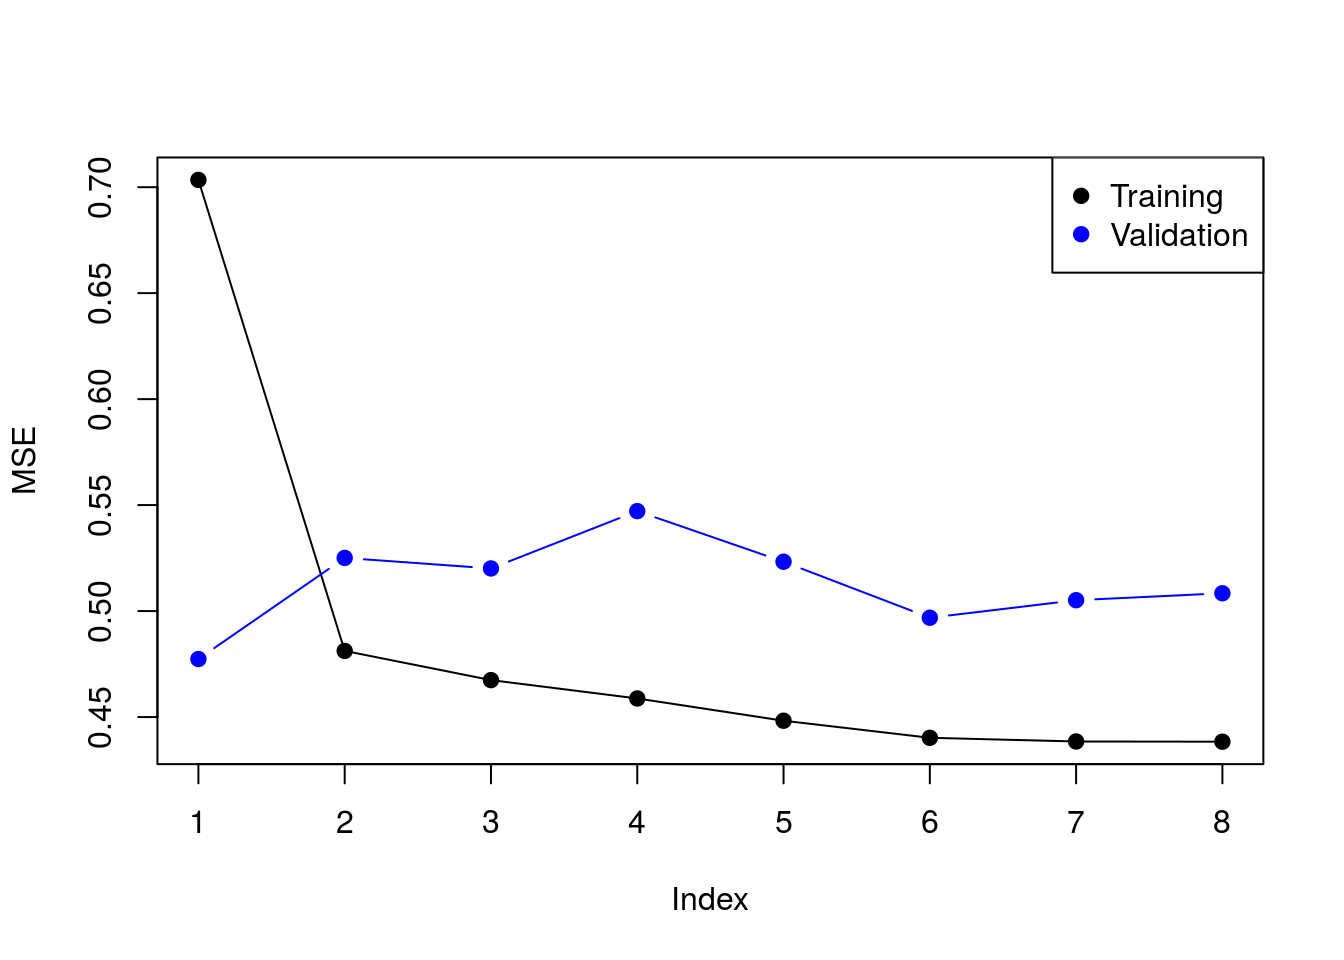
\includegraphics[width=0.5\linewidth]{Rcourse_files/figure-latex/unnamed-chunk-159-1}

Things to note:

\begin{itemize}
\tightlist
\item
  The bi-plot plots each data point along its PCs.
\item
  We used the \texttt{ggbiplot} function from the \textbf{ggbiplot}
  (available from github, but not from CRAN), because it has a nicer
  output than \texttt{stats::biplot}.
\item
  The bi-plot also plots the loadings as arrows. The coordinates of the
  arrows belong to the weight of each of the original variables in each
  PC. For example, the x-value of each arrow is the loadings on the
  first PC (on the x-axis). Since the weights of Murder, Assault, and
  Rape are almost the same, and larger then UrbanPop, we conclude that
  PC1 captures the average crime rate in each state.
\end{itemize}

The \emph{scree plot} depicts the quality of the approximation of \(X\)
as \(q\) grows. This is depicted using the proportion of variability in
\(X\) that is removed by each added PC. It is customary to choose \(q\)
as the first PC that has a relative low contribution to the
approximation of \(X\).

\begin{Shaded}
\begin{Highlighting}[]
\NormalTok{ggbiplot::}\KeywordTok{ggscreeplot}\NormalTok{(pca}\FloatTok{.1}\NormalTok{)}
\end{Highlighting}
\end{Shaded}

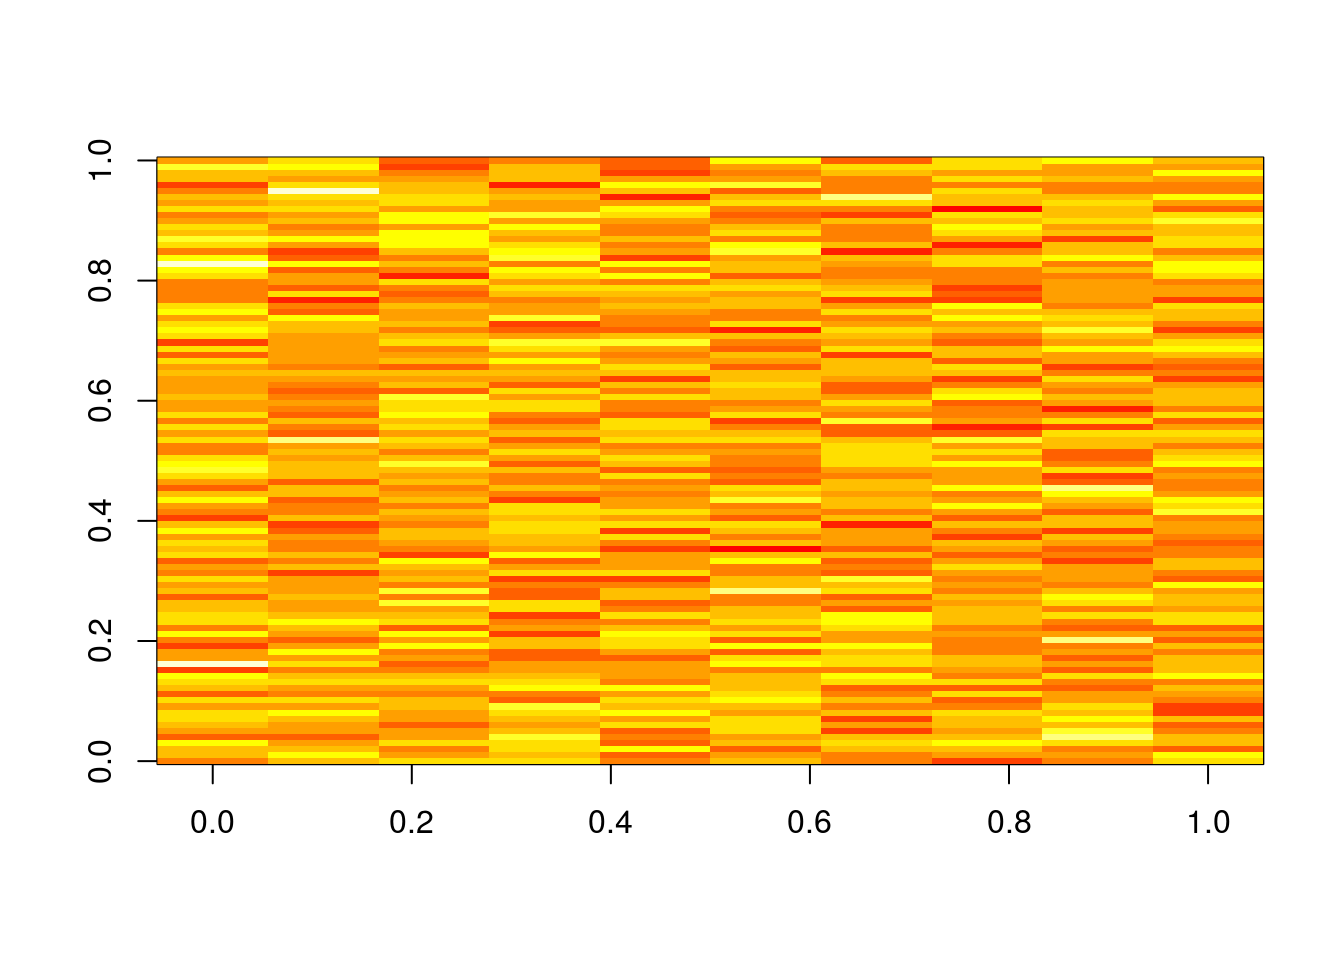
\includegraphics[width=0.5\linewidth]{Rcourse_files/figure-latex/unnamed-chunk-160-1}

See how the first PC captures the variability in the Assault levels and
Murder levels, with a single score.

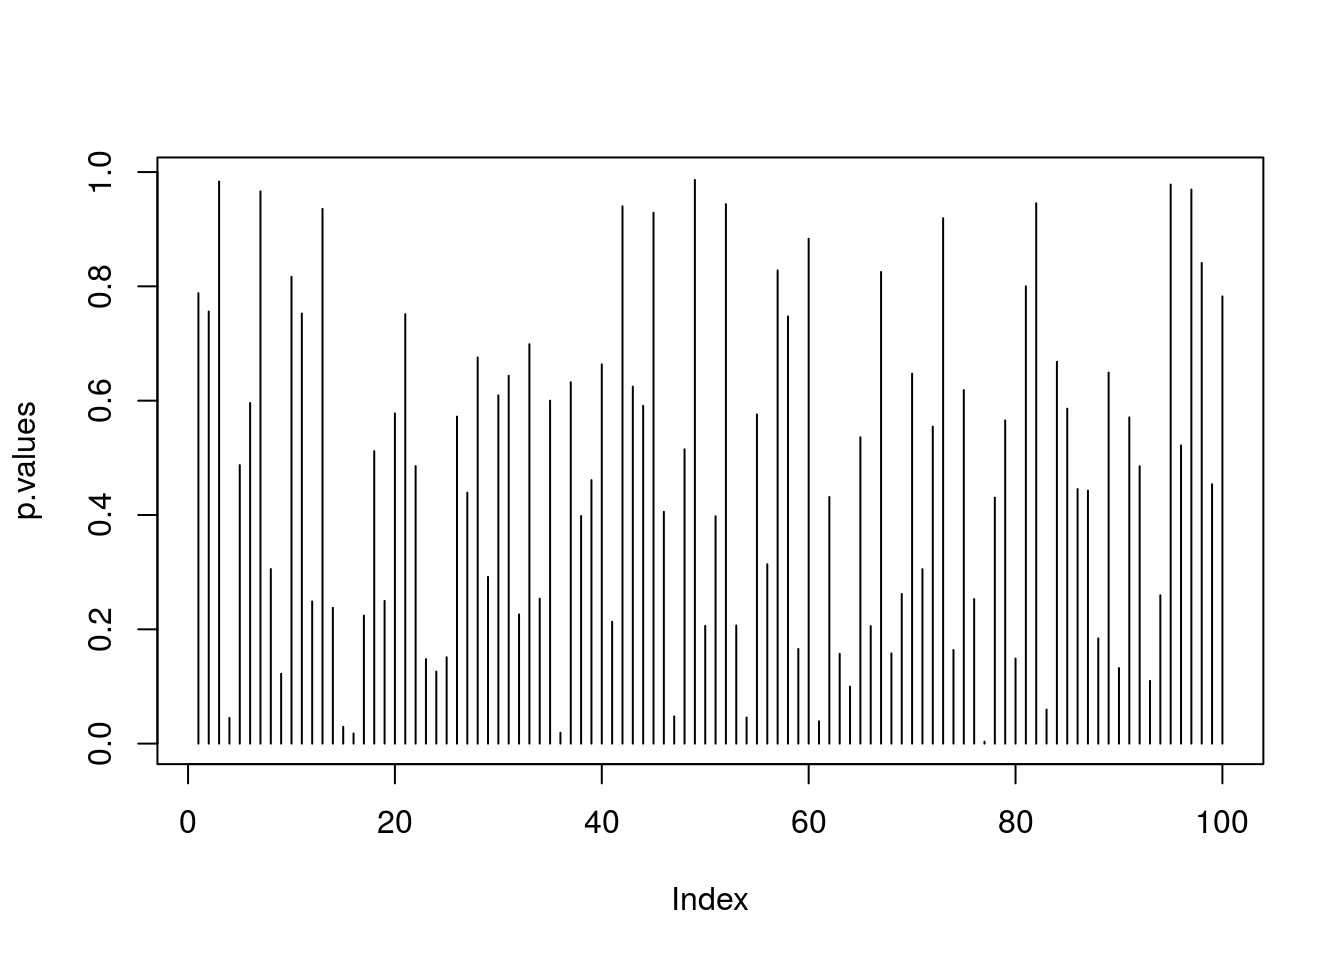
\includegraphics[width=0.5\linewidth]{Rcourse_files/figure-latex/unnamed-chunk-161-1}

More implementations of PCA:

\begin{Shaded}
\begin{Highlighting}[]
\CommentTok{# FAST solutions:}
\NormalTok{gmodels::}\KeywordTok{fast.prcomp}\NormalTok{()}

\CommentTok{# More detail in output:}
\NormalTok{FactoMineR::}\KeywordTok{PCA}\NormalTok{()}

\CommentTok{# For flexibility in algorithms and visualization:}
\NormalTok{ade4::}\KeywordTok{dudi.pca}\NormalTok{()}

\CommentTok{# Another one...}
\NormalTok{amap::}\KeywordTok{acp}\NormalTok{()}
\end{Highlighting}
\end{Shaded}

\subsubsection{FA}\label{fa}

\begin{Shaded}
\begin{Highlighting}[]
\NormalTok{fa}\FloatTok{.1} \NormalTok{<-}\StringTok{ }\NormalTok{psych::}\KeywordTok{principal}\NormalTok{(USArrests}\FloatTok{.1}\NormalTok{, }\DataTypeTok{nfactors =} \DecValTok{2}\NormalTok{, }\DataTypeTok{rotate =} \StringTok{"none"}\NormalTok{)}
\NormalTok{fa}\FloatTok{.1}
\end{Highlighting}
\end{Shaded}

\begin{verbatim}
## Principal Components Analysis
## Call: psych::principal(r = USArrests.1, nfactors = 2, rotate = "none")
## Standardized loadings (pattern matrix) based upon correlation matrix
##          PC1   PC2   h2     u2 com
## Murder  0.89 -0.36 0.93 0.0688 1.3
## Assault 0.93 -0.14 0.89 0.1072 1.0
## Rape    0.83  0.55 0.99 0.0073 1.7
## 
##                        PC1  PC2
## SS loadings           2.36 0.46
## Proportion Var        0.79 0.15
## Cumulative Var        0.79 0.94
## Proportion Explained  0.84 0.16
## Cumulative Proportion 0.84 1.00
## 
## Mean item complexity =  1.4
## Test of the hypothesis that 2 components are sufficient.
## 
## The root mean square of the residuals (RMSR) is  0.05 
##  with the empirical chi square  0.87  with prob <  NA 
## 
## Fit based upon off diagonal values = 0.99
\end{verbatim}

\begin{Shaded}
\begin{Highlighting}[]
\KeywordTok{biplot}\NormalTok{(fa}\FloatTok{.1}\NormalTok{, }\DataTypeTok{labels =}  \KeywordTok{rownames}\NormalTok{(USArrests}\FloatTok{.1}\NormalTok{)) }
\end{Highlighting}
\end{Shaded}

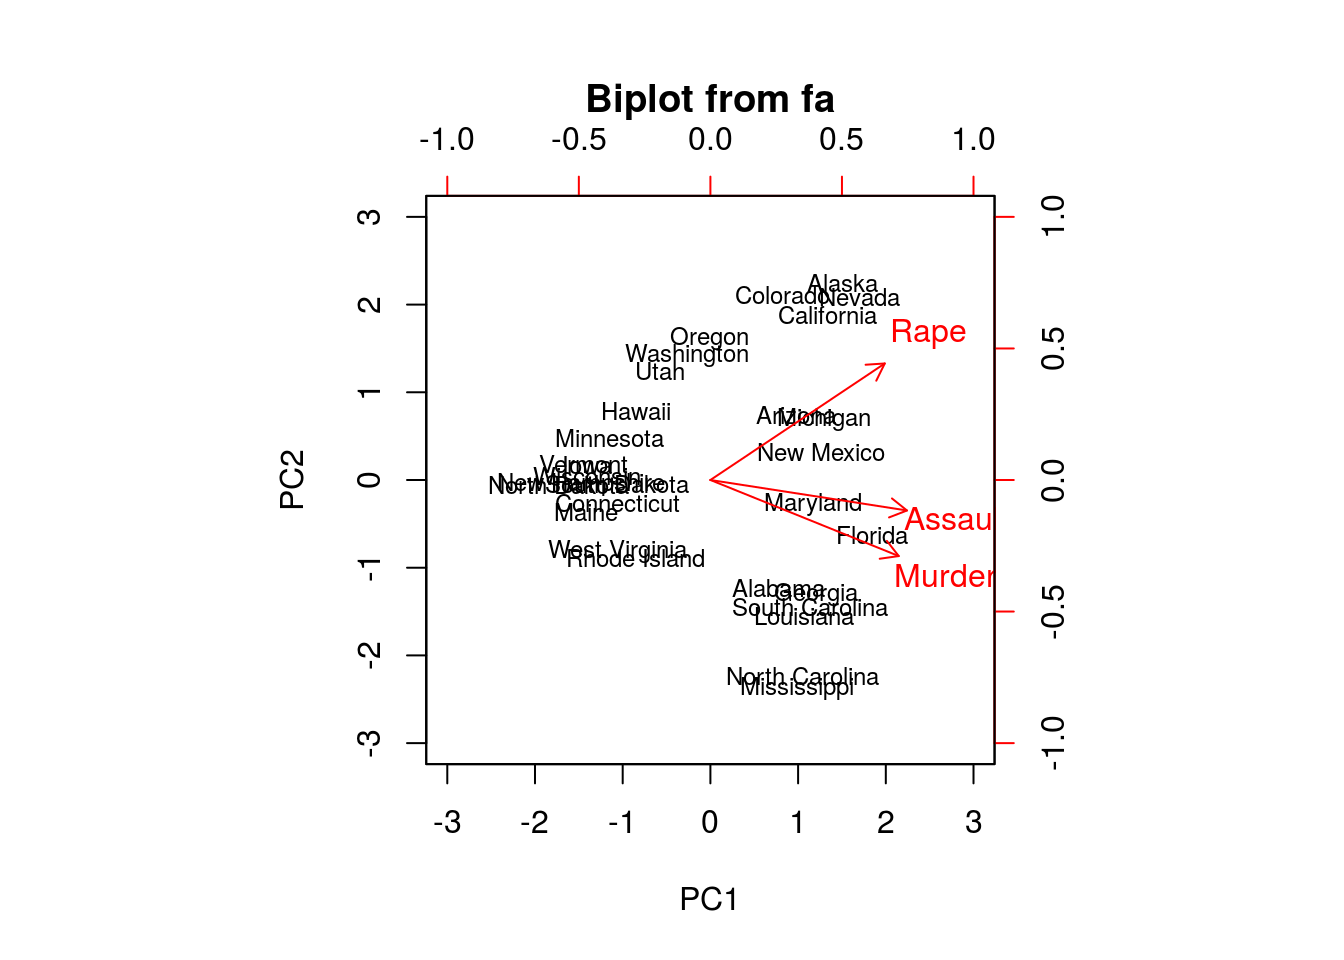
\includegraphics[width=0.5\linewidth]{Rcourse_files/figure-latex/FA-1}

\begin{Shaded}
\begin{Highlighting}[]
\CommentTok{# Numeric comparison with PCA:}
\NormalTok{fa}\FloatTok{.1}\NormalTok{$loadings}
\end{Highlighting}
\end{Shaded}

\begin{verbatim}
## 
## Loadings:
##         PC1    PC2   
## Murder   0.895 -0.361
## Assault  0.934 -0.145
## Rape     0.828  0.554
## 
##                  PC1   PC2
## SS loadings    2.359 0.458
## Proportion Var 0.786 0.153
## Cumulative Var 0.786 0.939
\end{verbatim}

\begin{Shaded}
\begin{Highlighting}[]
\NormalTok{pca}\FloatTok{.1}\NormalTok{$rotation}
\end{Highlighting}
\end{Shaded}

\begin{verbatim}
##                PC1        PC2        PC3
## Murder  -0.5826006  0.5339532 -0.6127565
## Assault -0.6079818  0.2140236  0.7645600
## Rape    -0.5393836 -0.8179779 -0.1999436
\end{verbatim}

Things to note:

\begin{itemize}
\tightlist
\item
  We perform FA with the \texttt{psych::principal} function.
\item
  The first factor (\texttt{fa.1\$loadings}) has different weights than
  the first PC (\texttt{pca.1\$rotation}) because of normalization. They
  are the same, however, in that the first PC, and the first factor,
  capture average crime levels.
\end{itemize}

Graphical model fans will like the following plot, where the
contribution of each variable to each factor is encoded in the width of
the arrow.

\begin{Shaded}
\begin{Highlighting}[]
\CommentTok{# Graph comparison: loadings encoded in colors}
\NormalTok{qgraph::}\KeywordTok{qgraph}\NormalTok{(fa}\FloatTok{.1}\NormalTok{)}
\end{Highlighting}
\end{Shaded}

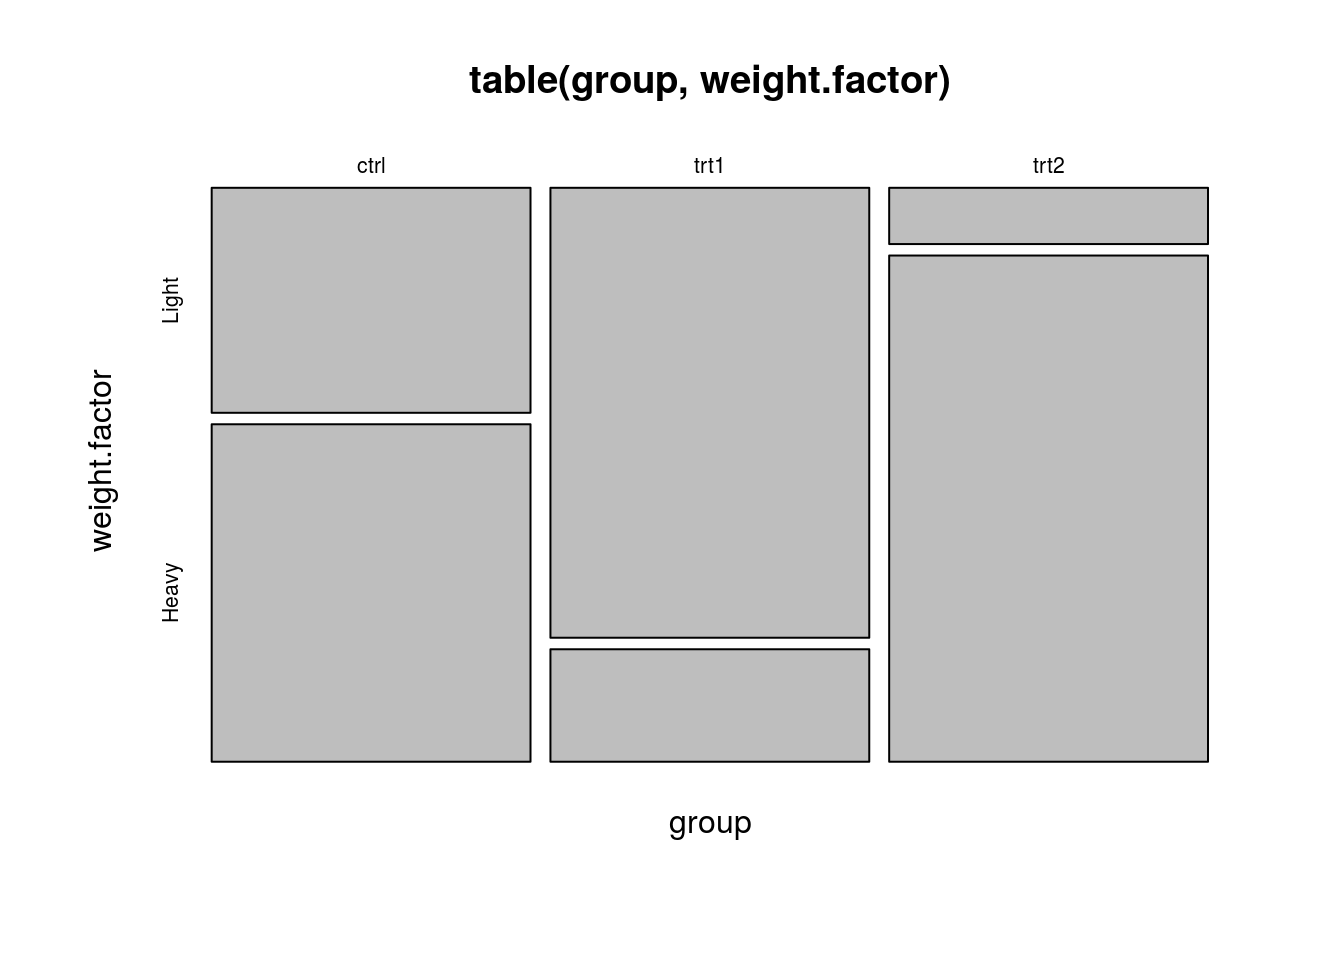
\includegraphics[width=0.5\linewidth]{Rcourse_files/figure-latex/unnamed-chunk-162-1}

Let's add a rotation (Varimax), and note that the rotation has indeed
changed the loadings of the variables, thus the interpretation of the
factors.

\begin{Shaded}
\begin{Highlighting}[]
\NormalTok{fa}\FloatTok{.2} \NormalTok{<-}\StringTok{ }\NormalTok{psych::}\KeywordTok{principal}\NormalTok{(USArrests}\FloatTok{.1}\NormalTok{, }\DataTypeTok{nfactors =} \DecValTok{2}\NormalTok{, }\DataTypeTok{rotate =} \StringTok{"varimax"}\NormalTok{)}

\NormalTok{fa}\FloatTok{.2}\NormalTok{$loadings}
\end{Highlighting}
\end{Shaded}

\begin{verbatim}
## 
## Loadings:
##         RC1   RC2  
## Murder  0.930 0.257
## Assault 0.829 0.453
## Rape    0.321 0.943
## 
##                  RC1   RC2
## SS loadings    1.656 1.160
## Proportion Var 0.552 0.387
## Cumulative Var 0.552 0.939
\end{verbatim}

\subsubsection{ICA}\label{ica}

\begin{Shaded}
\begin{Highlighting}[]
\NormalTok{ica}\FloatTok{.1} \NormalTok{<-}\StringTok{ }\NormalTok{fastICA::}\KeywordTok{fastICA}\NormalTok{(USArrests}\FloatTok{.1}\NormalTok{, }\DataTypeTok{n.com=}\DecValTok{2}\NormalTok{) }\CommentTok{# Also performs projection pursuit}

\KeywordTok{plot}\NormalTok{(ica}\FloatTok{.1}\NormalTok{$S)}
\KeywordTok{abline}\NormalTok{(}\DataTypeTok{h=}\DecValTok{0}\NormalTok{, }\DataTypeTok{v=}\DecValTok{0}\NormalTok{, }\DataTypeTok{lty=}\DecValTok{2}\NormalTok{)}
\KeywordTok{text}\NormalTok{(ica}\FloatTok{.1}\NormalTok{$S, }\DataTypeTok{pos =} \DecValTok{4}\NormalTok{, }\DataTypeTok{labels =} \KeywordTok{rownames}\NormalTok{(USArrests}\FloatTok{.1}\NormalTok{))}

\CommentTok{# Compare with two PCA (first two PCs):}
\KeywordTok{arrows}\NormalTok{(}\DataTypeTok{x0 =} \NormalTok{ica}\FloatTok{.1}\NormalTok{$S[,}\DecValTok{1}\NormalTok{], }\DataTypeTok{y0 =} \NormalTok{ica}\FloatTok{.1}\NormalTok{$S[,}\DecValTok{2}\NormalTok{], }\DataTypeTok{x1 =} \NormalTok{pca}\FloatTok{.1}\NormalTok{$x[,}\DecValTok{2}\NormalTok{], }\DataTypeTok{y1 =} \NormalTok{pca}\FloatTok{.1}\NormalTok{$x[,}\DecValTok{1}\NormalTok{], }\DataTypeTok{col=}\StringTok{'red'}\NormalTok{, }\DataTypeTok{pch=}\DecValTok{19}\NormalTok{, }\DataTypeTok{cex=}\FloatTok{0.5}\NormalTok{)}
\end{Highlighting}
\end{Shaded}

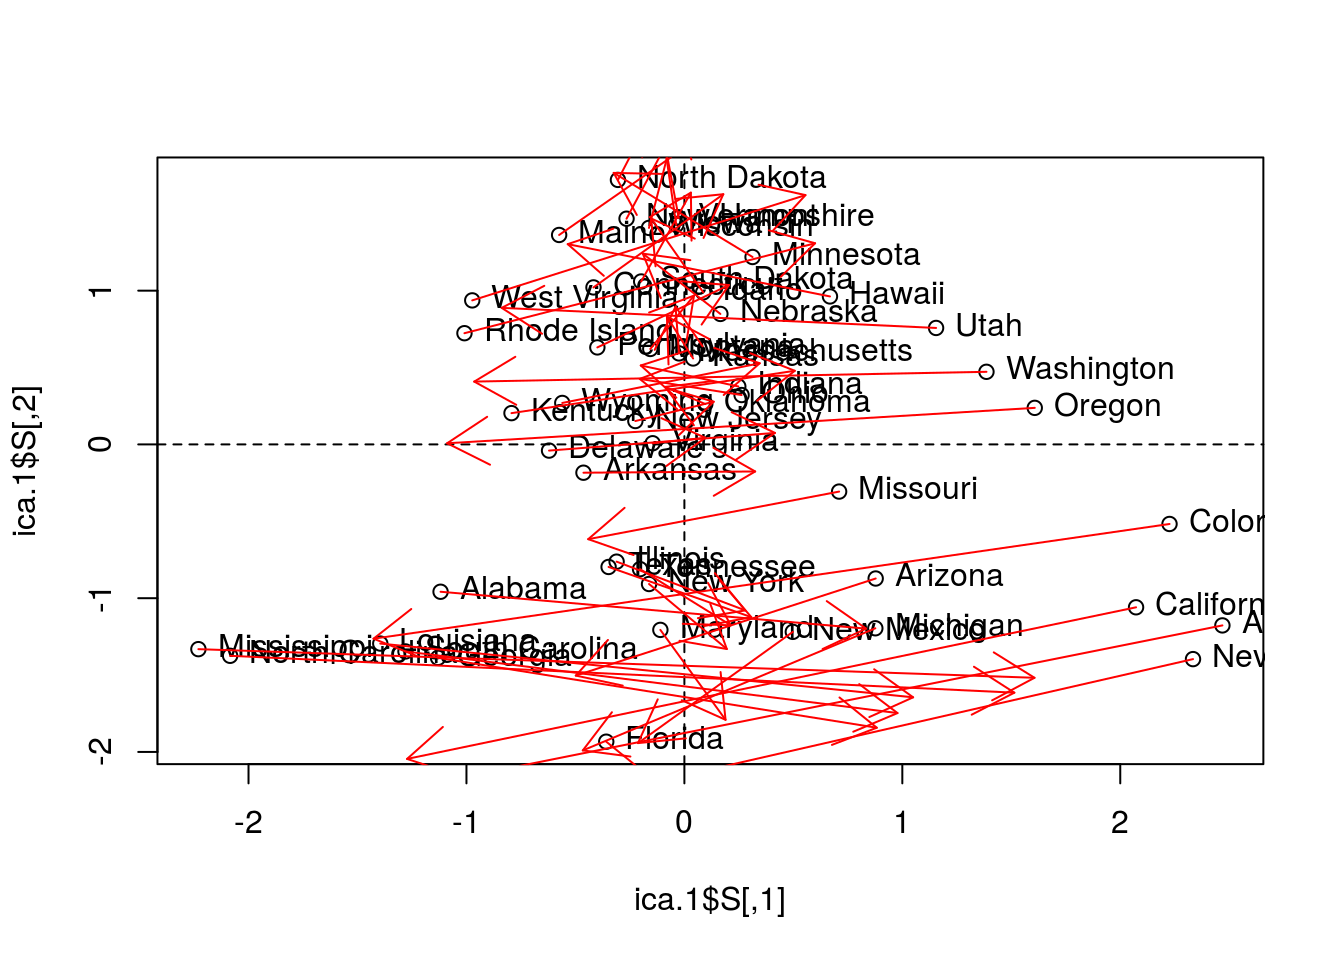
\includegraphics[width=0.5\linewidth]{Rcourse_files/figure-latex/ICA-1}

Things to note:

\begin{itemize}
\tightlist
\item
  ICA is fitted with \texttt{fastICA::fastICA}.
\item
  The ICA components are very different than the PCA components.
\end{itemize}

\subsubsection{MDS}\label{mds}

Classical MDS, also compared with PCA.

\begin{Shaded}
\begin{Highlighting}[]
\CommentTok{# We first need a dissimarity matrix/graph:}
\NormalTok{state.disimilarity <-}\StringTok{ }\KeywordTok{dist}\NormalTok{(USArrests}\FloatTok{.1}\NormalTok{)}

\NormalTok{mds}\FloatTok{.1} \NormalTok{<-}\StringTok{ }\KeywordTok{cmdscale}\NormalTok{(state.disimilarity)}

\KeywordTok{plot}\NormalTok{(mds}\FloatTok{.1}\NormalTok{, }\DataTypeTok{pch =} \DecValTok{19}\NormalTok{)}
\KeywordTok{abline}\NormalTok{(}\DataTypeTok{h=}\DecValTok{0}\NormalTok{, }\DataTypeTok{v=}\DecValTok{0}\NormalTok{, }\DataTypeTok{lty=}\DecValTok{2}\NormalTok{)}
\NormalTok{USArrests}\FloatTok{.2} \NormalTok{<-}\StringTok{ }\NormalTok{USArrests[,}\DecValTok{1}\NormalTok{:}\DecValTok{2}\NormalTok{] %>%}\StringTok{  }\NormalTok{scale}
\KeywordTok{text}\NormalTok{(mds}\FloatTok{.1}\NormalTok{, }\DataTypeTok{pos =} \DecValTok{4}\NormalTok{, }\DataTypeTok{labels =} \KeywordTok{rownames}\NormalTok{(USArrests}\FloatTok{.2}\NormalTok{), }\DataTypeTok{col =} \StringTok{'tomato'}\NormalTok{)}

\CommentTok{# Compare with two PCA (first two PCs):}
\KeywordTok{points}\NormalTok{(pca}\FloatTok{.1}\NormalTok{$x[,}\DecValTok{1}\NormalTok{:}\DecValTok{2}\NormalTok{], }\DataTypeTok{col=}\StringTok{'red'}\NormalTok{, }\DataTypeTok{pch=}\DecValTok{19}\NormalTok{, }\DataTypeTok{cex=}\FloatTok{0.5}\NormalTok{)}
\end{Highlighting}
\end{Shaded}

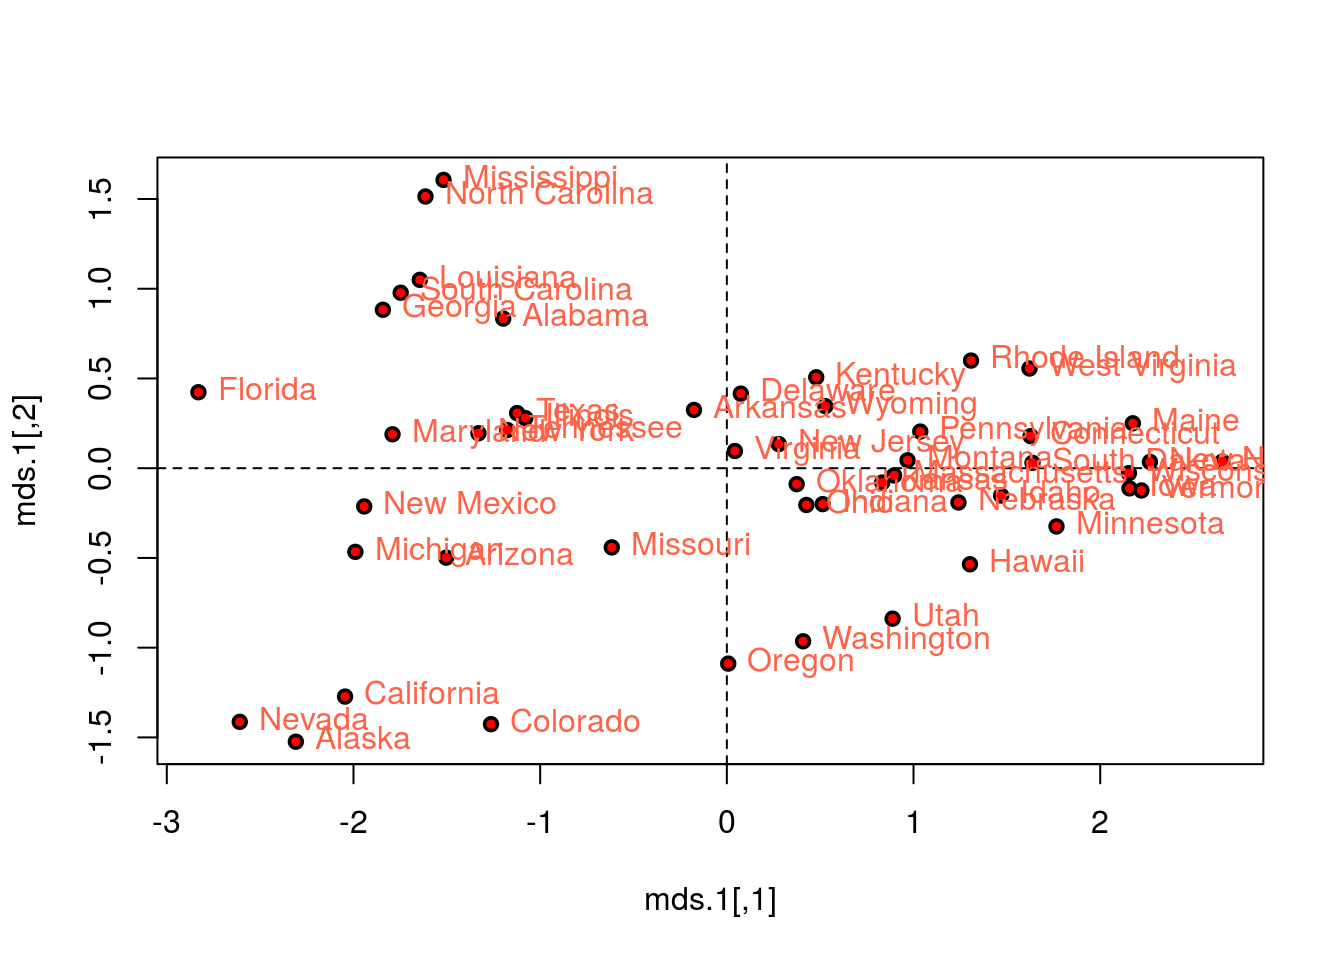
\includegraphics[width=0.5\linewidth]{Rcourse_files/figure-latex/MDS-1}

Things to note:

\begin{itemize}
\tightlist
\item
  For MDS, we first compute a dissimilarity graph with \texttt{dist},
  and then learn the embedding with \texttt{cmdscale}.
\item
  As previously stated, the embedding of PCA is the same as classical
  MDS with Euclidean distances.
\item
  See the \texttt{cluster::daisy} function for more dissimilarity
  measures.
\end{itemize}

Let's try other strain functions for MDS, like Sammon's strain, and
compare it with the PCs.

\begin{Shaded}
\begin{Highlighting}[]
\NormalTok{mds}\FloatTok{.2} \NormalTok{<-}\StringTok{ }\NormalTok{MASS::}\KeywordTok{sammon}\NormalTok{(state.disimilarity, }\DataTypeTok{trace =} \OtherTok{FALSE}\NormalTok{)}
\KeywordTok{plot}\NormalTok{(mds}\FloatTok{.2}\NormalTok{$points, }\DataTypeTok{pch =} \DecValTok{19}\NormalTok{)}
\KeywordTok{abline}\NormalTok{(}\DataTypeTok{h=}\DecValTok{0}\NormalTok{, }\DataTypeTok{v=}\DecValTok{0}\NormalTok{, }\DataTypeTok{lty=}\DecValTok{2}\NormalTok{)}
\KeywordTok{text}\NormalTok{(mds}\FloatTok{.2}\NormalTok{$points, }\DataTypeTok{pos =} \DecValTok{4}\NormalTok{, }\DataTypeTok{labels =} \KeywordTok{rownames}\NormalTok{(USArrests}\FloatTok{.2}\NormalTok{))}

\CommentTok{# Compare with two PCA (first two PCs):}
\KeywordTok{arrows}\NormalTok{(}
  \DataTypeTok{x0 =} \NormalTok{mds}\FloatTok{.2}\NormalTok{$points[,}\DecValTok{1}\NormalTok{], }\DataTypeTok{y0 =} \NormalTok{mds}\FloatTok{.2}\NormalTok{$points[,}\DecValTok{2}\NormalTok{], }
  \DataTypeTok{x1 =} \NormalTok{pca}\FloatTok{.1}\NormalTok{$x[,}\DecValTok{1}\NormalTok{], }\DataTypeTok{y1 =} \NormalTok{pca}\FloatTok{.1}\NormalTok{$x[,}\DecValTok{2}\NormalTok{], }
  \DataTypeTok{col=}\StringTok{'red'}\NormalTok{, }\DataTypeTok{pch=}\DecValTok{19}\NormalTok{, }\DataTypeTok{cex=}\FloatTok{0.5}\NormalTok{)}
\end{Highlighting}
\end{Shaded}

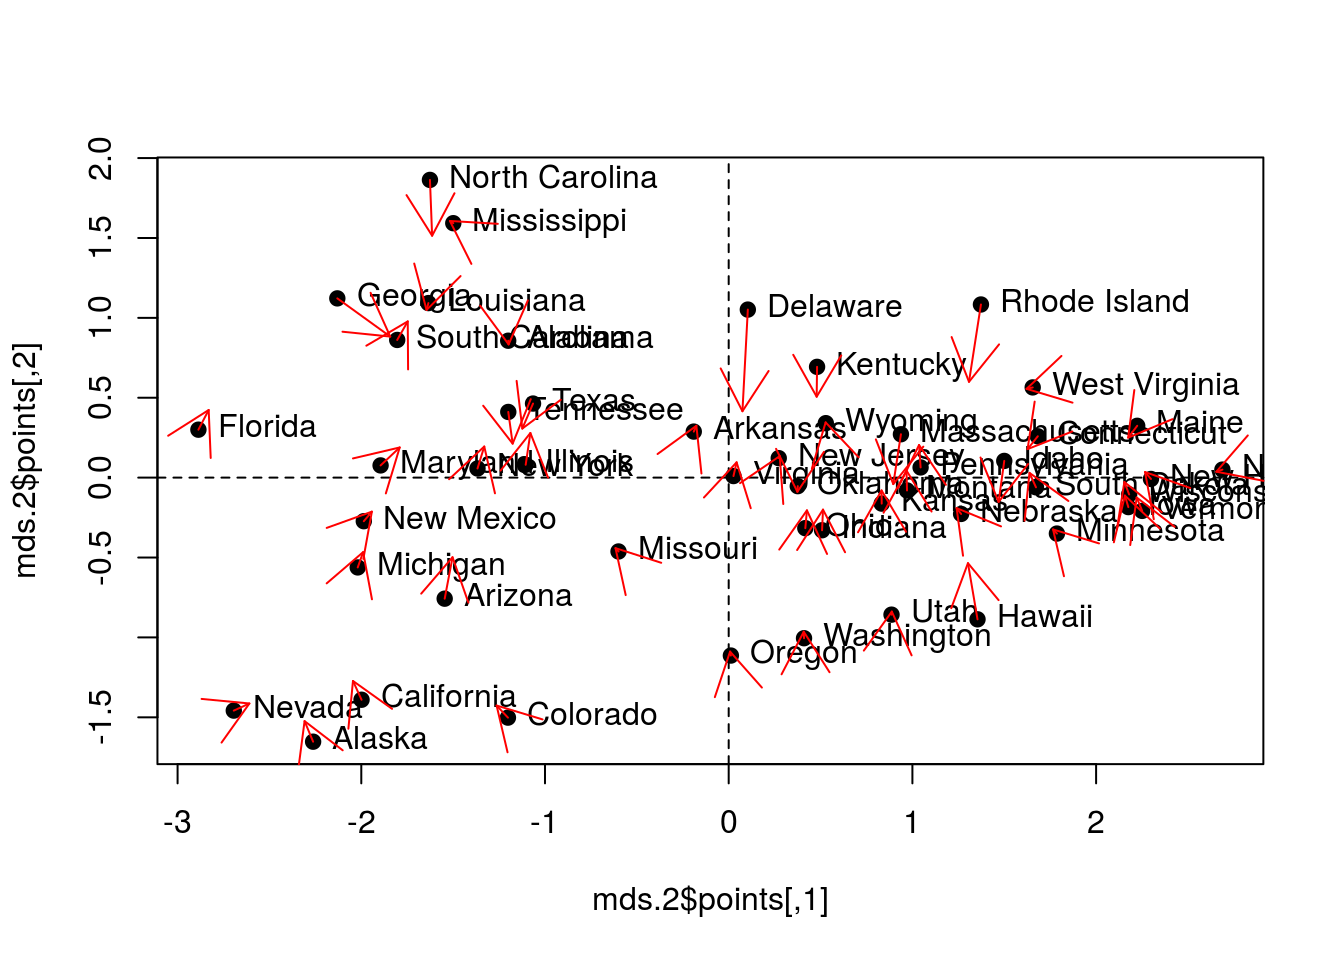
\includegraphics[width=0.5\linewidth]{Rcourse_files/figure-latex/SammonMDS-1}

Things to note:

\begin{itemize}
\tightlist
\item
  \texttt{MASS::sammon} does the fitting.
\item
  The embedding returned by the Sammon strain is different than that of
  the first two PCs.
\end{itemize}

\subsubsection{Sparse PCA}\label{sparse-pca}

\begin{Shaded}
\begin{Highlighting}[]
\CommentTok{# Compute similarity graph}
\NormalTok{state.similarity <-}\StringTok{ }\NormalTok{MASS::}\KeywordTok{cov.rob}\NormalTok{(USArrests}\FloatTok{.1}\NormalTok{)$cov}

\NormalTok{spca1 <-}\StringTok{ }\NormalTok{elasticnet::}\KeywordTok{spca}\NormalTok{(state.similarity, }\DataTypeTok{K=}\DecValTok{2}\NormalTok{, }\DataTypeTok{type=}\StringTok{"Gram"}\NormalTok{, }\DataTypeTok{sparse=}\StringTok{"penalty"}\NormalTok{, }\DataTypeTok{trace=}\OtherTok{FALSE}\NormalTok{, }\DataTypeTok{para=}\KeywordTok{c}\NormalTok{(}\FloatTok{0.06}\NormalTok{,}\FloatTok{0.16}\NormalTok{))}
\NormalTok{spca1$loadings}
\end{Highlighting}
\end{Shaded}

\begin{verbatim}
##                PC1 PC2
## Murder  -0.7143088   0
## Assault -0.2023409  -1
## Rape    -0.6699411   0
\end{verbatim}

\subsubsection{Kernel PCA}\label{kernel-pca-1}

\begin{Shaded}
\begin{Highlighting}[]
\NormalTok{kernlab::}\KeywordTok{kpca}\NormalTok{()}
\end{Highlighting}
\end{Shaded}

\section{Clustering}\label{cluster}

\BeginKnitrBlock{example}
\protect\hypertarget{ex:photos}{}{\label{ex:photos}}Consider the tagging of
your friends' pictures on Facebook. If you tagged some pictures,
Facebook may try to use a supervised approach to automatically label
photos. If you never tagged pictures, a supervised approach is
impossible. It is still possible to group simiar pictures together.
\EndKnitrBlock{example}

\BeginKnitrBlock{example}
\protect\hypertarget{ex:spam}{}{\label{ex:spam}}Consider the problem of spam
detection. It would be nice if each user could label several thousands
emails, to apply a supervised learning approach to spam detection. This
is an unrealistic demand, so a pre-clustering stage is useful: the user
only needs to tag a couple dozens of homogenous clusters, before solving
the supervisedl learning problem.
\EndKnitrBlock{example}

In clustering problems, we seek to group observations that are similar.

There are many motivations for clustering:

\begin{enumerate}
\def\labelenumi{\arabic{enumi}.}
\tightlist
\item
  \textbf{Understanding}: The most common use of clustering is probably
  as a an exploratory step, to identify homogeneous groups in the data.
\item
  \textbf{Dimensionality reduction}: Clustering may be seen as a method
  for dimensionality reduction. Unlike the approaches in the
  Dimensionality Reduction Section \ref{dim-reduce}, it does not
  ``compress'' variables but rather observations. Each group of
  homogeneous observations may then be represented as a single
  prototypical observation of the group.
\item
  \textbf{Pre-Labelling}: Clustering may be performed as a
  pre-processing step for supervised learning, when labeling all the
  samples is impossible due to ``budget'' constraints, like in Example
  \ref{ex:spam}. This is sometimes known as \emph{pre-clustering}.
\end{enumerate}

Clustering, like dimensionality reduction, may rely on some latent
variable generative model, or on purely algorithmic approaches.

\subsection{Latent Variable
Approaches}\label{latent-variable-approaches-1}

\subsubsection{Finite Mixture}\label{finite-mixture}

\BeginKnitrBlock{example}
\protect\hypertarget{ex:males-females}{}{\label{ex:males-females}}Consider
the distribution of heights in some population. Given the gender,
heights have a nice bell shaped distribution. If genders have not been
recorded, We can view it as a \emph{latent}, i.e., unobservale, with
\(K=2\) levels: males and females.
\EndKnitrBlock{example}

A \emph{finite mixture} is the marginal distribution of \(K\) distinct
classes, when the class variable is \emph{latent}. This is useful for
clustering since we can assume the number of classes, \(K\), and the
distribution of each class. We can then use maximum likelihood
estimation to fit the mixture distribution and assign observations to
the most probable class.

\subsection{Purely Algorithmic
Approaches}\label{purely-algorithmic-approaches-1}

\subsubsection{K-means}\label{k-means}

The \emph{K-means} algorithm is possibly the most popular clustering
algorithm. The goal behind K-means clustering algorithm is finding a
representative point for each of K clusters, and assign each data point
to one of these clusters. As each cluster has a representative point,
this is also a \emph{prototype method} The clusters are defined so that
they minimize the average Euclidean distance between all points to the
center of the cluster.

In K-means, the clusters are first defined, and then similarities
computed. This is thus a \emph{top-down} method.

K-means clustering requires the raw features \(X\) as inputs, and not
only a similarity graph. This is evident when examining the algorithm
below.

The k-means algorithm works as follows:

\begin{enumerate}
\def\labelenumi{\arabic{enumi}.}
\tightlist
\item
  Choose the number of clusters \(K\).
\item
  Arbitrarily assign points to clusters.
\item
  While clusters keep changing:

  \begin{enumerate}
  \def\labelenumii{\arabic{enumii}.}
  \tightlist
  \item
    Compute the cluster centers as the average of their points.
  \item
    Assign each point to its closest cluster center (in Euclidean
    distance).
  \end{enumerate}
\item
  Return Cluster assignments and means.
\end{enumerate}

\BeginKnitrBlock{remark}
\iffalse {Remark. } \fi If are trained as a statistician, you may
wonder- what population quantity is K-means actually estimating? The
estimand of K-means is known as the \emph{K principal points}. Principal
points are points which are \emph{self consistent}, i.e., they are the
mean of their neighbourhood.
\EndKnitrBlock{remark}

\subsubsection{K-means++}\label{k-means-1}

\emph{K-means++} is a fast version of K-means thanks to a smart
initialization.

\subsubsection{K-medoids}\label{k-medoids}

If a Euclidean distance is inappropriate for a particular set of
variables, or that robustness to corrupt observations is required, or
that we wish to constrain the cluster centers to be actual observations,
then the \emph{K-Medoids} algorithm is an adaptation of K-means that
allows this. It is also known under the name \emph{partition around
medoids} (PAM) clustering.

The k-medoids algorithm works as follows.

\begin{enumerate}
\def\labelenumi{\arabic{enumi}.}
\tightlist
\item
  Given a dissimilarity graph.
\item
  Choose the number of clusters \(K\).
\item
  Arbitrarily assign points to clusters.
\item
  While clusters keep changing:

  \begin{enumerate}
  \def\labelenumii{\arabic{enumii}.}
  \tightlist
  \item
    Within each cluster, set the center as the data point that minimizes
    the sum of distances to other points in the cluster.
  \item
    Assign each point to its closest cluster center.
  \end{enumerate}
\item
  Return Cluster assignments and centers.
\end{enumerate}

\subsubsection{Hirarchial Clustering}\label{hirarchial-clustering}

Hierarchical clustering algorithms take dissimilarity graphs as inputs.
Hierarchical clustering is a class of greedy \emph{graph-partitioning}
algorithms. Being hierarchical by design, they have the attractive
property that the evolution of the clustering can be presented with a
\emph{dendogram}, i.e., a tree plot.\\
A particular advantage of these methods is that they do not require an
a-priori choice of the number of cluster (\(K\)).

Two main sub-classes of algorithms are \emph{agglomerative}, and
\emph{divisive}.

\emph{Agglomerative clustering} algorithms are \textbf{bottom-up}
algorithm which build clusters by joining smaller clusters. To decide
which clusters are joined at each iteration some measure of closeness
between clusters is required.

\begin{itemize}
\tightlist
\item
  \textbf{Single Linkage}: Cluster distance is defined by the distance
  between the two \textbf{closest} members.
\item
  \textbf{Complete Linkage}: Cluster distance is defined by the distance
  between the two \textbf{farthest} members.
\item
  \textbf{Group Average}: Cluster distance is defined by the
  \textbf{average} distance between members.
\item
  \textbf{Group Median}: Like Group Average, only using the median.
\end{itemize}

\emph{Divisive clustering} algorithms are \textbf{top-down} algorithm
which build clusters by splitting larger clusters.

\subsubsection{Fuzzy Clustering}\label{fuzzy-clustering}

Can be thought of as a purely algorithmic view of the finite-mixture in
Section \ref{finite-mixture}.

\subsection{Clustering in R}\label{clustering-in-r}

\subsubsection{K-Means}\label{k-means-2}

The following code is an adaptation from
\href{http://people.stat.sc.edu/Hitchcock/chapter6_R_examples.txt}{David
Hitchcock}.

\begin{Shaded}
\begin{Highlighting}[]
\NormalTok{k <-}\StringTok{ }\DecValTok{2}
\NormalTok{kmeans}\FloatTok{.1} \NormalTok{<-}\StringTok{ }\NormalTok{stats::}\KeywordTok{kmeans}\NormalTok{(USArrests}\FloatTok{.1}\NormalTok{, }\DataTypeTok{centers =} \NormalTok{k)}
\KeywordTok{head}\NormalTok{(kmeans}\FloatTok{.1}\NormalTok{$cluster) }\CommentTok{# cluster asignments}
\end{Highlighting}
\end{Shaded}

\begin{verbatim}
##    Alabama     Alaska    Arizona   Arkansas California   Colorado 
##          1          1          1          2          1          1
\end{verbatim}

\begin{Shaded}
\begin{Highlighting}[]
\CommentTok{# Visualize using scatter plots of the original features}
\KeywordTok{pairs}\NormalTok{(USArrests}\FloatTok{.1}\NormalTok{, }\DataTypeTok{panel=}\NormalTok{function(x,y) }\KeywordTok{text}\NormalTok{(x,y,kmeans}\FloatTok{.1}\NormalTok{$cluster))}
\end{Highlighting}
\end{Shaded}

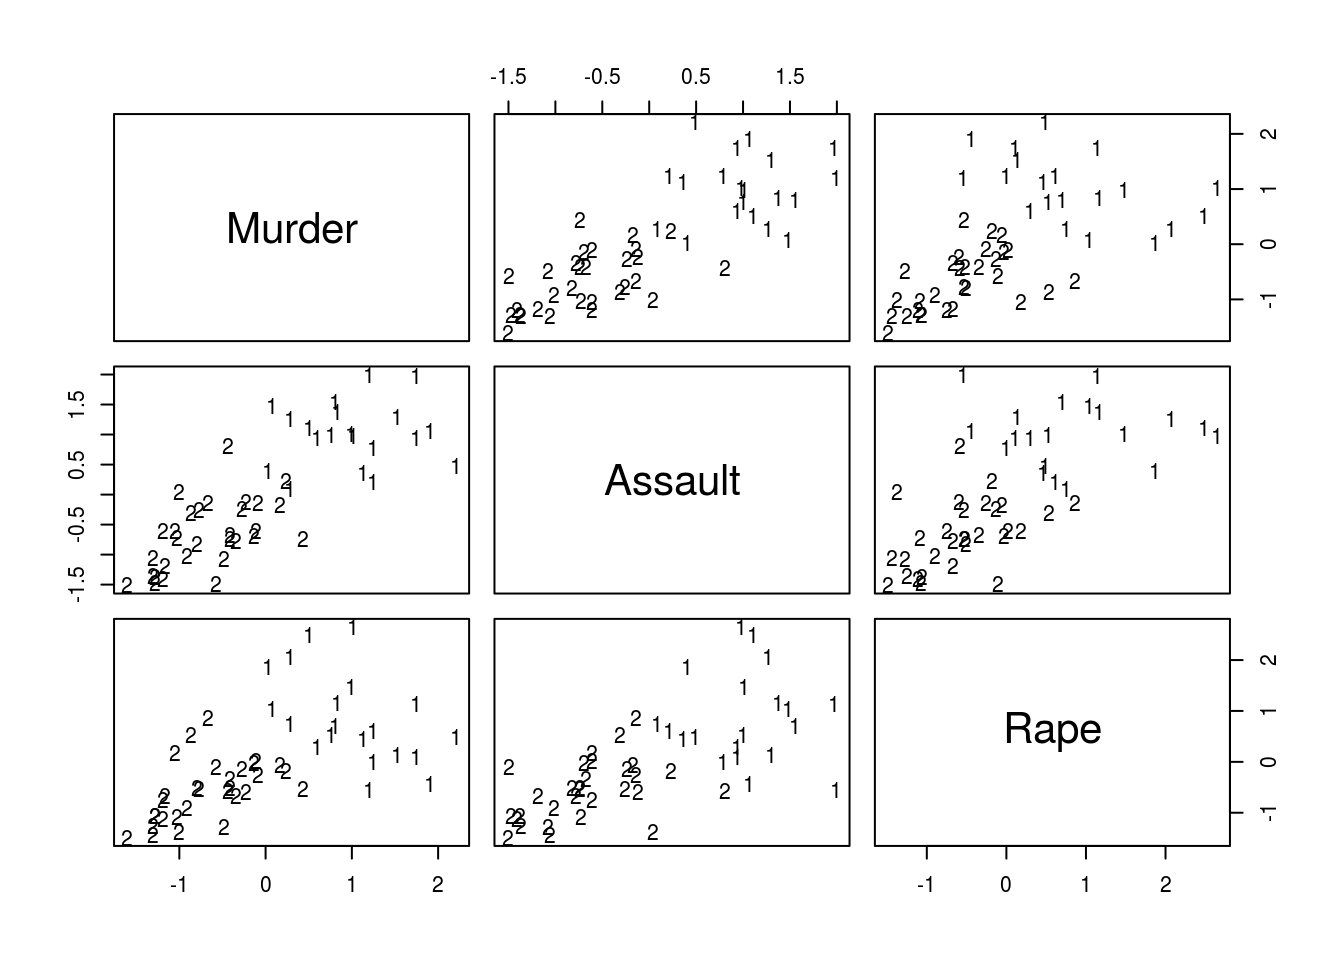
\includegraphics[width=0.5\linewidth]{Rcourse_files/figure-latex/kmeans-1}

Things to note:

\begin{itemize}
\tightlist
\item
  The \texttt{stats::kmeans} function does the clustering.
\item
  The cluster assignment is given in the \texttt{cluster} element of the
  \texttt{stats::kmeans} output.
\item
  The visual inspection confirms that similar states have been assigned
  to the same cluster.
\end{itemize}

\subsubsection{K-means ++}\label{k-means-3}

\emph{K-Means++} is a smart initialization for K-Means. The following
code is taken from the
\href{https://stat.ethz.ch/pipermail/r-help/2012-January/300051.html}{r-help}
mailing list.

\begin{Shaded}
\begin{Highlighting}[]
\CommentTok{# Write my own K-means++ function.}
\NormalTok{kmpp <-}\StringTok{ }\NormalTok{function(X, k) \{}
  
  \NormalTok{n <-}\StringTok{ }\KeywordTok{nrow}\NormalTok{(X)}
  \NormalTok{C <-}\StringTok{ }\KeywordTok{numeric}\NormalTok{(k)}
  \NormalTok{C[}\DecValTok{1}\NormalTok{] <-}\StringTok{ }\KeywordTok{sample}\NormalTok{(}\DecValTok{1}\NormalTok{:n, }\DecValTok{1}\NormalTok{)}
  
  \NormalTok{for (i in }\DecValTok{2}\NormalTok{:k) \{}
    \NormalTok{dm <-}\StringTok{ }\NormalTok{pracma::}\KeywordTok{distmat}\NormalTok{(X, X[C, ])}
    \NormalTok{pr <-}\StringTok{ }\KeywordTok{apply}\NormalTok{(dm, }\DecValTok{1}\NormalTok{, min); pr[C] <-}\StringTok{ }\DecValTok{0}
    \NormalTok{C[i] <-}\StringTok{ }\KeywordTok{sample}\NormalTok{(}\DecValTok{1}\NormalTok{:n, }\DecValTok{1}\NormalTok{, }\DataTypeTok{prob =} \NormalTok{pr)}
  \NormalTok{\}}
  
  \KeywordTok{kmeans}\NormalTok{(X, X[C, ])}
\NormalTok{\}}

\CommentTok{# Examine output:}
\NormalTok{kmeans}\FloatTok{.2} \NormalTok{<-}\StringTok{ }\KeywordTok{kmpp}\NormalTok{(USArrests}\FloatTok{.1}\NormalTok{, k)}
\KeywordTok{head}\NormalTok{(kmeans}\FloatTok{.2}\NormalTok{$cluster)}
\end{Highlighting}
\end{Shaded}

\begin{verbatim}
##    Alabama     Alaska    Arizona   Arkansas California   Colorado 
##          1          1          1          2          1          1
\end{verbatim}

\subsubsection{K-medoids}\label{k-medoids-1}

\begin{Shaded}
\begin{Highlighting}[]
\NormalTok{state.disimilarity <-}\StringTok{ }\KeywordTok{dist}\NormalTok{(USArrests}\FloatTok{.1}\NormalTok{)}
\NormalTok{kmed}\FloatTok{.1} \NormalTok{<-}\StringTok{ }\NormalTok{cluster::}\KeywordTok{pam}\NormalTok{(}\DataTypeTok{x=} \NormalTok{state.disimilarity, }\DataTypeTok{k=}\DecValTok{2}\NormalTok{)}
\KeywordTok{head}\NormalTok{(kmed}\FloatTok{.1}\NormalTok{$clustering)}
\end{Highlighting}
\end{Shaded}

\begin{verbatim}
##    Alabama     Alaska    Arizona   Arkansas California   Colorado 
##          1          1          1          1          1          1
\end{verbatim}

\begin{Shaded}
\begin{Highlighting}[]
\KeywordTok{plot}\NormalTok{(pca}\FloatTok{.1}\NormalTok{$x[,}\DecValTok{1}\NormalTok{], pca}\FloatTok{.1}\NormalTok{$x[,}\DecValTok{2}\NormalTok{], }\DataTypeTok{xlab=}\StringTok{"PC 1"}\NormalTok{, }\DataTypeTok{ylab=}\StringTok{"PC 2"}\NormalTok{, }\DataTypeTok{type =}\StringTok{'n'}\NormalTok{, }\DataTypeTok{lwd=}\DecValTok{2}\NormalTok{)}
\KeywordTok{text}\NormalTok{(pca}\FloatTok{.1}\NormalTok{$x[,}\DecValTok{1}\NormalTok{], pca}\FloatTok{.1}\NormalTok{$x[,}\DecValTok{2}\NormalTok{], }\DataTypeTok{labels=}\KeywordTok{rownames}\NormalTok{(USArrests}\FloatTok{.1}\NormalTok{), }\DataTypeTok{cex=}\FloatTok{0.7}\NormalTok{, }\DataTypeTok{lwd=}\DecValTok{2}\NormalTok{, }\DataTypeTok{col=}\NormalTok{kmed}\FloatTok{.1}\NormalTok{$cluster)}
\end{Highlighting}
\end{Shaded}

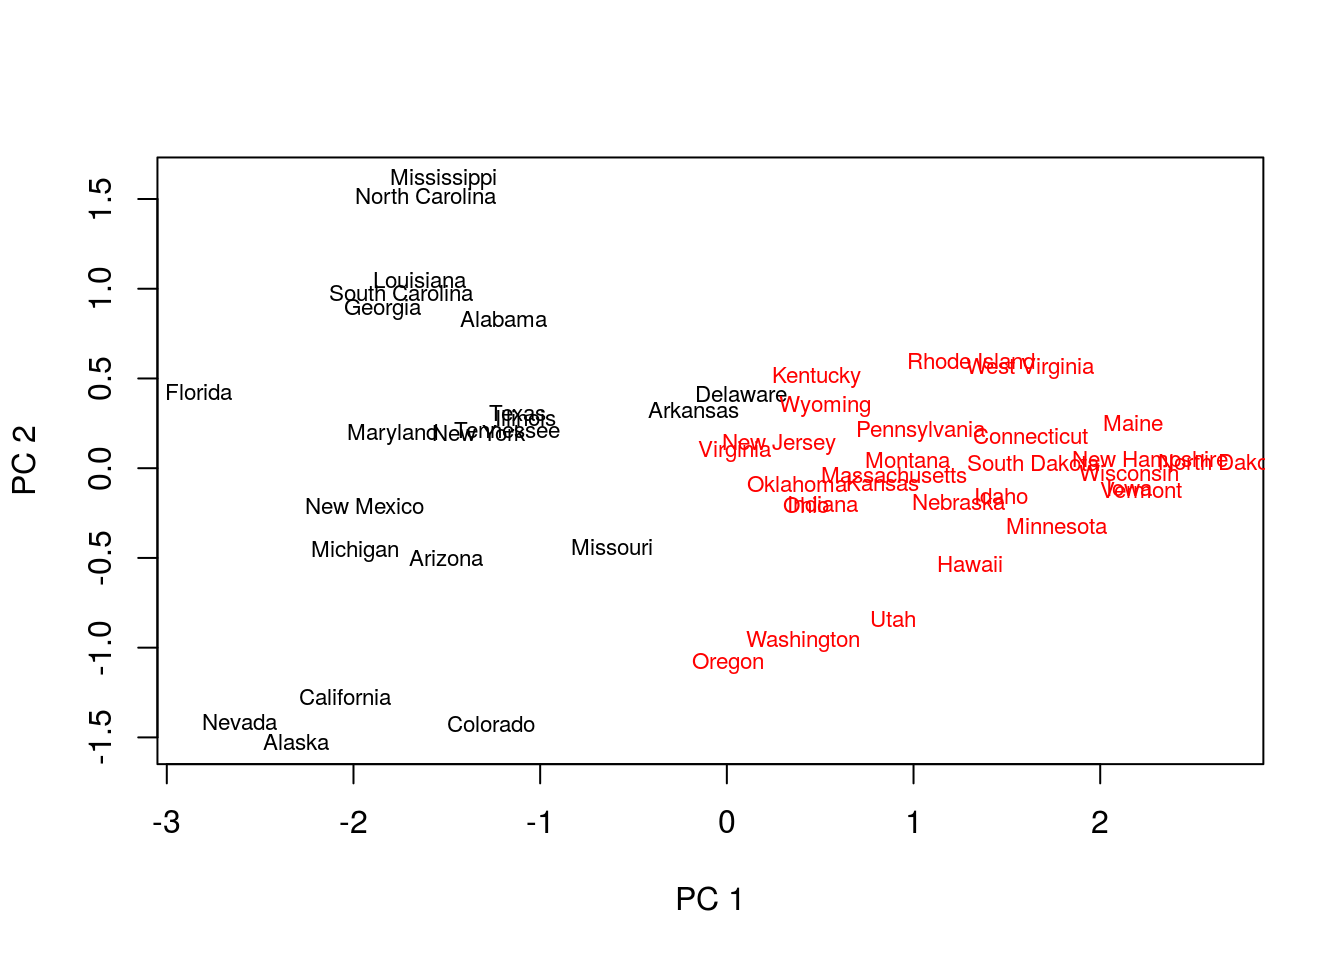
\includegraphics[width=0.5\linewidth]{Rcourse_files/figure-latex/kmedoids-1}

Things to note:

\begin{itemize}
\tightlist
\item
  K-medoids starts with the computation of a dissimilarity graph, done
  by the \texttt{dist} function.
\item
  The clustering is done by the \texttt{cluster::pam} function.
\item
  Inspecting the output confirms that similar states have been assigned
  to the same cluster.
\item
  Many other similarity measures can be found in \texttt{proxy::dist()}.
\item
  See \texttt{cluster::clara()} for a big-data implementation of PAM.
\end{itemize}

\subsubsection{Hirarchial Clustering}\label{hirarchial-clustering-1}

We start with agglomerative clustering with single-linkage.

\begin{Shaded}
\begin{Highlighting}[]
\CommentTok{# Single linkage:}
\NormalTok{hirar}\FloatTok{.1} \NormalTok{<-}\StringTok{ }\KeywordTok{hclust}\NormalTok{(state.disimilarity, }\DataTypeTok{method=}\StringTok{'single'}\NormalTok{)}
\KeywordTok{plot}\NormalTok{(hirar}\FloatTok{.1}\NormalTok{, }\DataTypeTok{labels=}\KeywordTok{rownames}\NormalTok{(USArrests}\FloatTok{.1}\NormalTok{), }\DataTypeTok{ylab=}\StringTok{"Distance"}\NormalTok{)}
\end{Highlighting}
\end{Shaded}

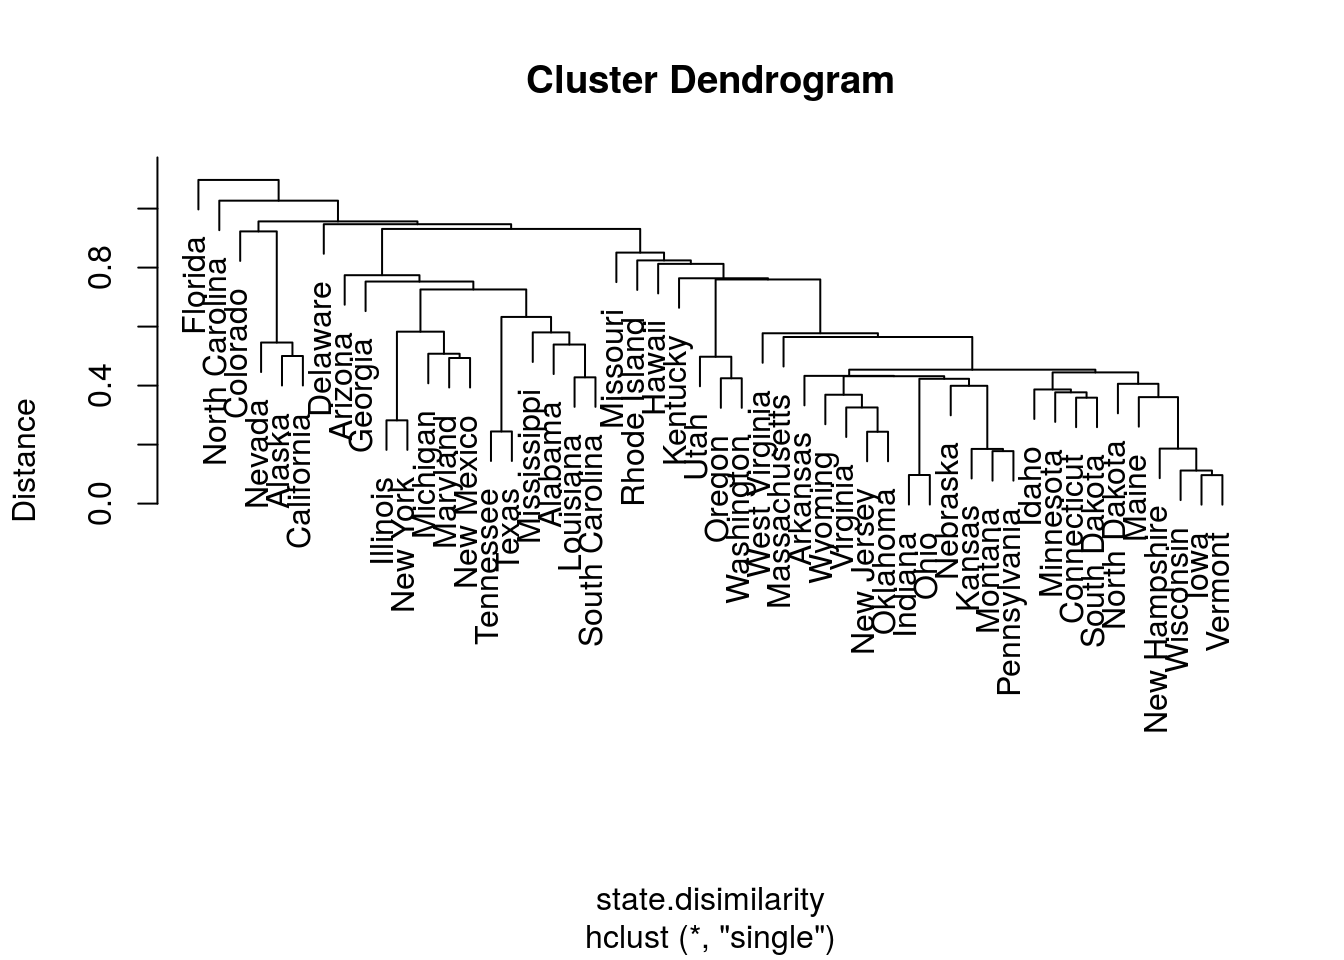
\includegraphics[width=0.5\linewidth]{Rcourse_files/figure-latex/HirarchialClustering-1}

Things to note:

\begin{itemize}
\tightlist
\item
  The clustering is done with the \texttt{hclust} function.
\item
  We choose the single-linkage distance using the
  \texttt{method=\textquotesingle{}single\textquotesingle{}} argument.
\item
  We did not need to a-priori specify the number of clusters, \(K\).
\item
  The \texttt{plot} function has a particular method for \texttt{hclust}
  class objects, and plots them as dendograms.
\end{itemize}

We not try other types of linkages, to verify that the indeed affect the
clustering.

\begin{Shaded}
\begin{Highlighting}[]
\CommentTok{# Complete linkage:}
\NormalTok{hirar}\FloatTok{.2} \NormalTok{<-}\StringTok{ }\KeywordTok{hclust}\NormalTok{(state.disimilarity, }\DataTypeTok{method=}\StringTok{'complete'}\NormalTok{)}
\KeywordTok{plot}\NormalTok{(hirar}\FloatTok{.2}\NormalTok{, }\DataTypeTok{labels=}\KeywordTok{rownames}\NormalTok{(USArrests}\FloatTok{.1}\NormalTok{), }\DataTypeTok{ylab=}\StringTok{"Distance"}\NormalTok{)}
\end{Highlighting}
\end{Shaded}

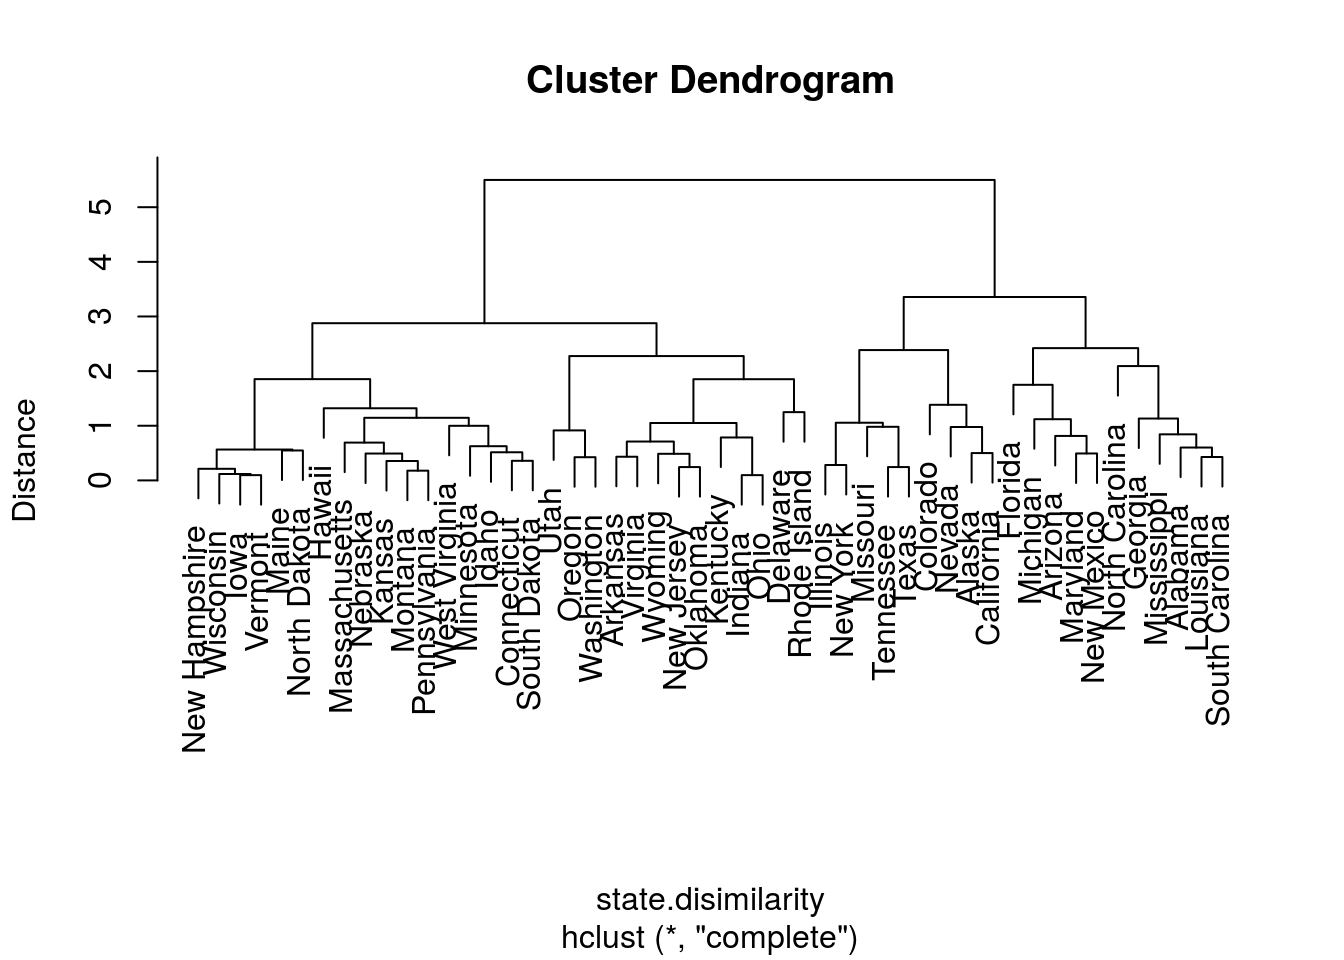
\includegraphics[width=0.5\linewidth]{Rcourse_files/figure-latex/unnamed-chunk-164-1}

\begin{Shaded}
\begin{Highlighting}[]
\CommentTok{# Average linkage:}
\NormalTok{hirar}\FloatTok{.3} \NormalTok{<-}\StringTok{ }\KeywordTok{hclust}\NormalTok{(state.disimilarity, }\DataTypeTok{method=}\StringTok{'average'}\NormalTok{)}
\KeywordTok{plot}\NormalTok{(hirar}\FloatTok{.3}\NormalTok{, }\DataTypeTok{labels=}\KeywordTok{rownames}\NormalTok{(USArrests}\FloatTok{.1}\NormalTok{), }\DataTypeTok{ylab=}\StringTok{"Distance"}\NormalTok{)}
\end{Highlighting}
\end{Shaded}

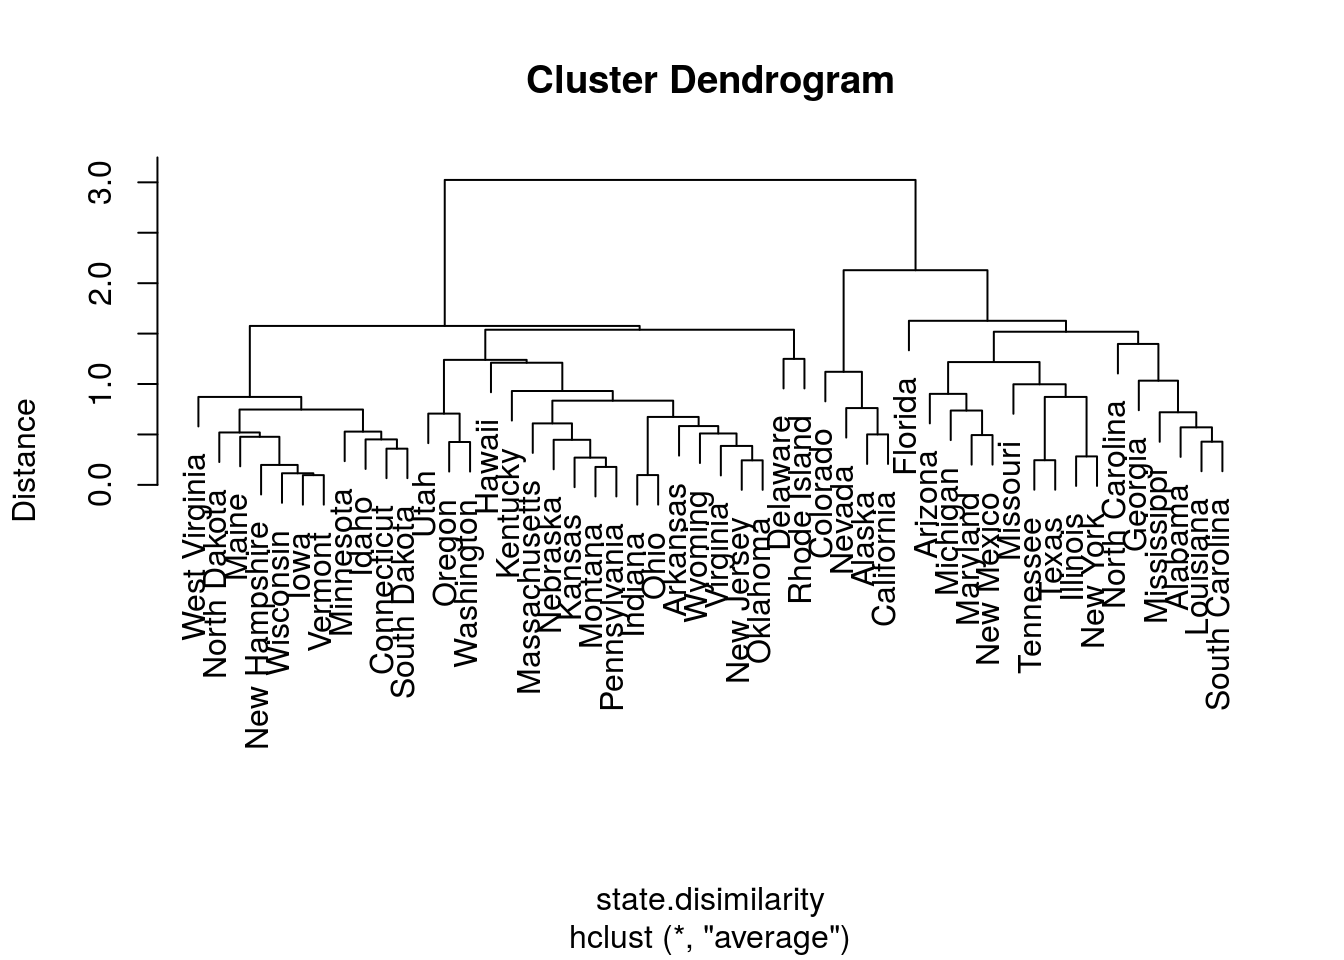
\includegraphics[width=0.5\linewidth]{Rcourse_files/figure-latex/unnamed-chunk-164-2}

If we know how many clusters we want, we can use \texttt{cuttree} to get
the class assignments.

\begin{Shaded}
\begin{Highlighting}[]
\CommentTok{# Fixing the number of clusters:}
\NormalTok{cut}\FloatTok{.2.2} \NormalTok{<-}\StringTok{ }\KeywordTok{cutree}\NormalTok{(hirar}\FloatTok{.2}\NormalTok{, }\DataTypeTok{k=}\DecValTok{2}\NormalTok{)}
\KeywordTok{head}\NormalTok{(cut}\FloatTok{.2.2}\NormalTok{)   }\CommentTok{# printing the "clustering vector"}
\end{Highlighting}
\end{Shaded}

\begin{verbatim}
##    Alabama     Alaska    Arizona   Arkansas California   Colorado 
##          1          1          1          2          1          1
\end{verbatim}

\section{Bibliographic Notes}\label{bibliographic-notes-7}

For more on PCA see my
\href{https://github.com/johnros/dim_reduce/blob/master/dim_reduce.pdf}{Dimensionality
Reduction Class Notes} and references therein. For more on everything,
see \citet{friedman2001elements}. For a softer introduction, see
\citet{james2013introduction}.

\chapter{Plotting}\label{plotting}

Whether you are doing EDA, or preparing your results for publication,
you need plots. R has many plotting mechanisms, allowing the user a
tremendous amount of flexibility, while abstracting away a lot of the
tedious details. To be concrete, many of the plots in R are simply
impossible to produce with Excel, SPSS, or SAS, and would take a
tremendous amount of work to produce with Python, Java and lower level
programming languages.

In this text, we will focus on two plotting packages. The basic
\textbf{graphics} package, distributed with the base R distribution, and
the \textbf{ggplot2} package.

Before going into the details of the plotting packages, we start with
some high-level philosophy. The \textbf{graphics} package originates
from the main-frame days. Computers had no graphical interface, and the
output of the plot was immediately sent to a printer. For this reason,
once a plot has been produced with the \textbf{graphics} package, it
cannot be queryied nor changed, except for further additions.

The philosophy of R is that \textbf{everyting is an object}. The
\textbf{graphics} package does not adhere to this philosophy, and indeed
it was soon augmented with the \textbf{grid} package \citep{Rlanguage},
that treats plots as objects. \textbf{grid} is a low level graphics
interface, and users may be more familiar with the \textbf{lattice}
package built upon it \citep{lattice}.

\textbf{lattice} is very powerful, but soon enough, it was overtaken in
popularity by the \textbf{ggplot2} package \citep{ggplot2}.
\textbf{ggplot2} was the PhD project of \href{http://hadley.nz/}{Hadley
Wickham}, a name to remember\ldots{} Two fundamental ideas underlay
\textbf{ggplot2}: (i) everything is an object, and (ii), plots can be
described by a small set of building blocks. The building blocks in
\textbf{ggplot2} are the ones stated by \citet{wilkinson2006grammar}.
The objects and grammar of \textbf{ggplot2} have later evolved to allow
more complicated plotting and in particular, interactive plotting, in
other packages.

Interactive plotting is a very important feature for EDA, and for
reporting. The major leap in interactive plotting was made possible by
the advancement of web technologies, such as JavaScript. Why is this?
Because an interactive plot, or report, can be seen as a web-site.
Building upon the capabilities of JavaScript, and your web browser, to
provide the interactivity, greatly facilitates the development of such
plots, as the programmer can reply on the web-browsers capabilities for
interactivity.

One of the latest contributions to interactive plotting, is the
\textbf{Shiny} framework by RStudio \citep{shiny}. \textbf{Shiny},
unlike other interactive plotting systems, is not a static web-site. It
is a web-server, that can query R, with all its facilities.

\section{The graphics System}\label{the-graphics-system}

The R code from the Basics Chapter \ref{basics} is a demonstration of
the \textbf{graphics} package and system. We make a quick review of the
basics.

\subsection{Using Existing Plotting
Functions}\label{using-existing-plotting-functions}

\subsubsection{Scatter Plot}\label{scatter-plot}

A simple scatter plot.

\begin{Shaded}
\begin{Highlighting}[]
\KeywordTok{attach}\NormalTok{(trees)}
\KeywordTok{plot}\NormalTok{(Girth ~}\StringTok{ }\NormalTok{Height)}
\end{Highlighting}
\end{Shaded}

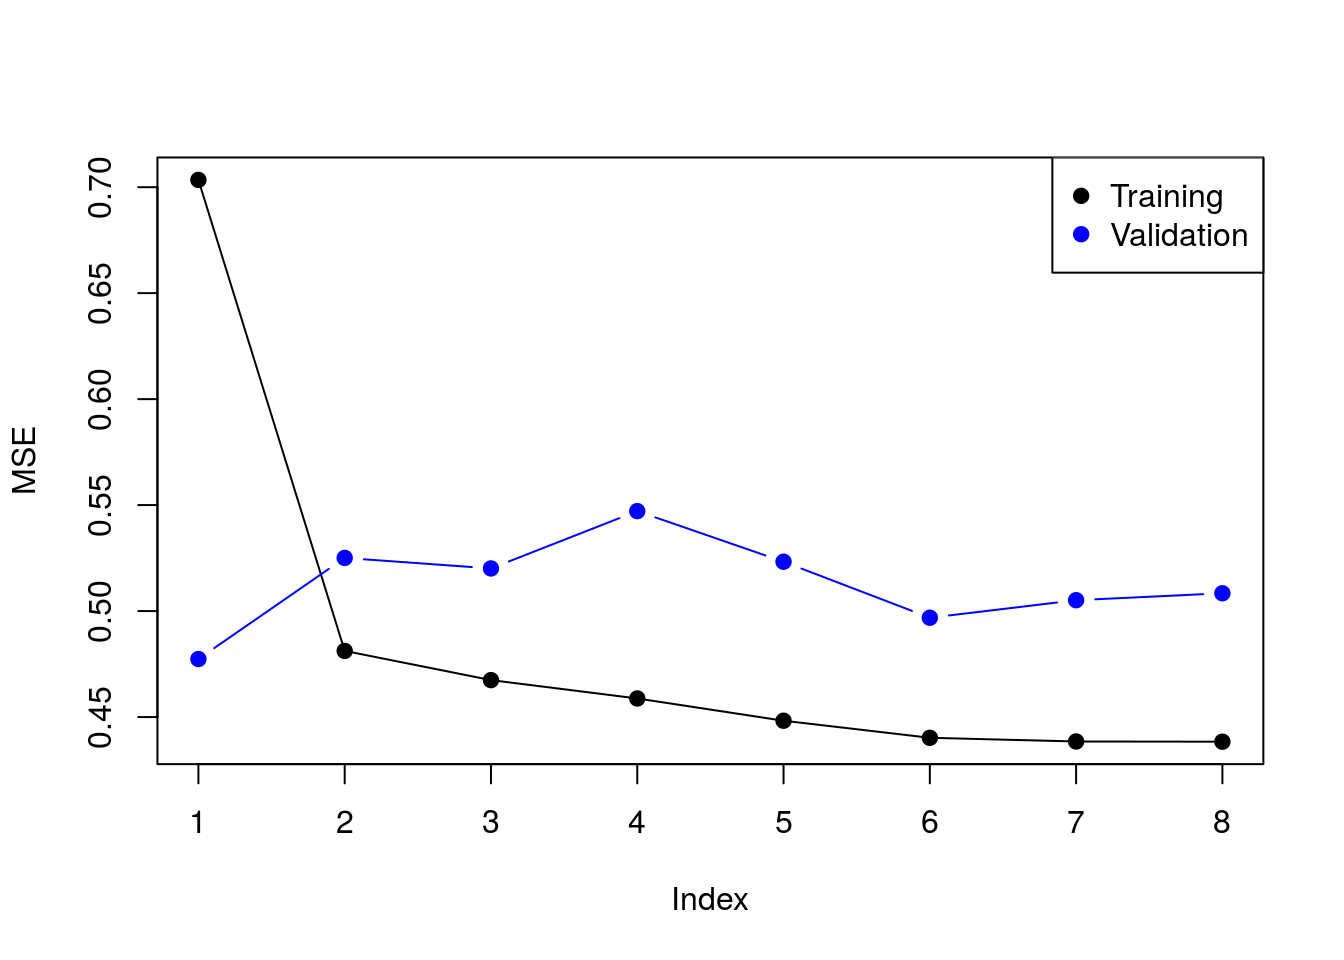
\includegraphics[width=0.5\linewidth]{Rcourse_files/figure-latex/unnamed-chunk-166-1}

Various types of plots.

\begin{Shaded}
\begin{Highlighting}[]
\KeywordTok{par}\NormalTok{(}\DataTypeTok{mfrow=}\KeywordTok{c}\NormalTok{(}\DecValTok{2}\NormalTok{,}\DecValTok{3}\NormalTok{))}
\KeywordTok{plot}\NormalTok{(Girth, }\DataTypeTok{type=}\StringTok{'h'}\NormalTok{, }\DataTypeTok{main=}\StringTok{"type='h'"}\NormalTok{) }
\KeywordTok{plot}\NormalTok{(Girth, }\DataTypeTok{type=}\StringTok{'o'}\NormalTok{, }\DataTypeTok{main=}\StringTok{"type='o'"}\NormalTok{) }
\KeywordTok{plot}\NormalTok{(Girth, }\DataTypeTok{type=}\StringTok{'l'}\NormalTok{, }\DataTypeTok{main=}\StringTok{"type='l'"}\NormalTok{)}
\KeywordTok{plot}\NormalTok{(Girth, }\DataTypeTok{type=}\StringTok{'s'}\NormalTok{, }\DataTypeTok{main=}\StringTok{"type='s'"}\NormalTok{)}
\KeywordTok{plot}\NormalTok{(Girth, }\DataTypeTok{type=}\StringTok{'b'}\NormalTok{, }\DataTypeTok{main=}\StringTok{"type='b'"}\NormalTok{)}
\KeywordTok{plot}\NormalTok{(Girth, }\DataTypeTok{type=}\StringTok{'p'}\NormalTok{, }\DataTypeTok{main=}\StringTok{"type='p'"}\NormalTok{)}
\end{Highlighting}
\end{Shaded}

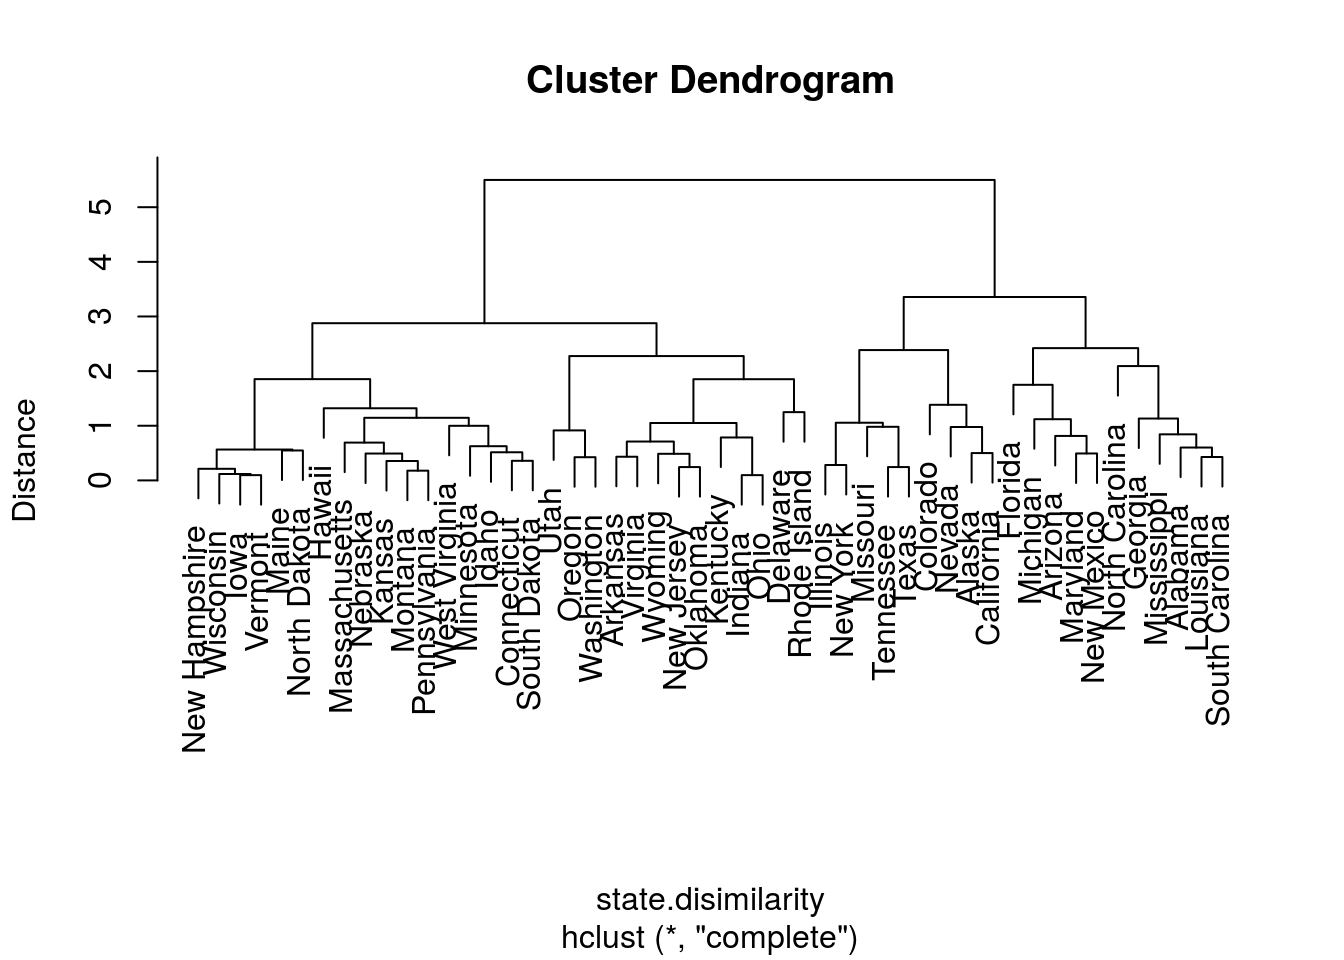
\includegraphics[width=0.5\linewidth]{Rcourse_files/figure-latex/unnamed-chunk-167-1}

\begin{Shaded}
\begin{Highlighting}[]
\KeywordTok{par}\NormalTok{(}\DataTypeTok{mfrow=}\KeywordTok{c}\NormalTok{(}\DecValTok{1}\NormalTok{,}\DecValTok{1}\NormalTok{))}
\end{Highlighting}
\end{Shaded}

Things to note:

\begin{itemize}
\tightlist
\item
  The \texttt{par} command controls the plotting parameters.
  \texttt{mfrow=c(2,3)} is used to produce a matrix of plots with 2 rows
  and 3 columns.
\item
  The \texttt{type} argument controls the type of plot.
\item
  The \texttt{main} argument controls the title.
\item
  See \texttt{?plot} and \texttt{?par} for more options.
\end{itemize}

Control the plotting characters with the \texttt{pch} argument.

\begin{Shaded}
\begin{Highlighting}[]
\KeywordTok{plot}\NormalTok{(Girth, }\DataTypeTok{pch=}\StringTok{'+'}\NormalTok{, }\DataTypeTok{cex=}\DecValTok{3}\NormalTok{)}
\end{Highlighting}
\end{Shaded}

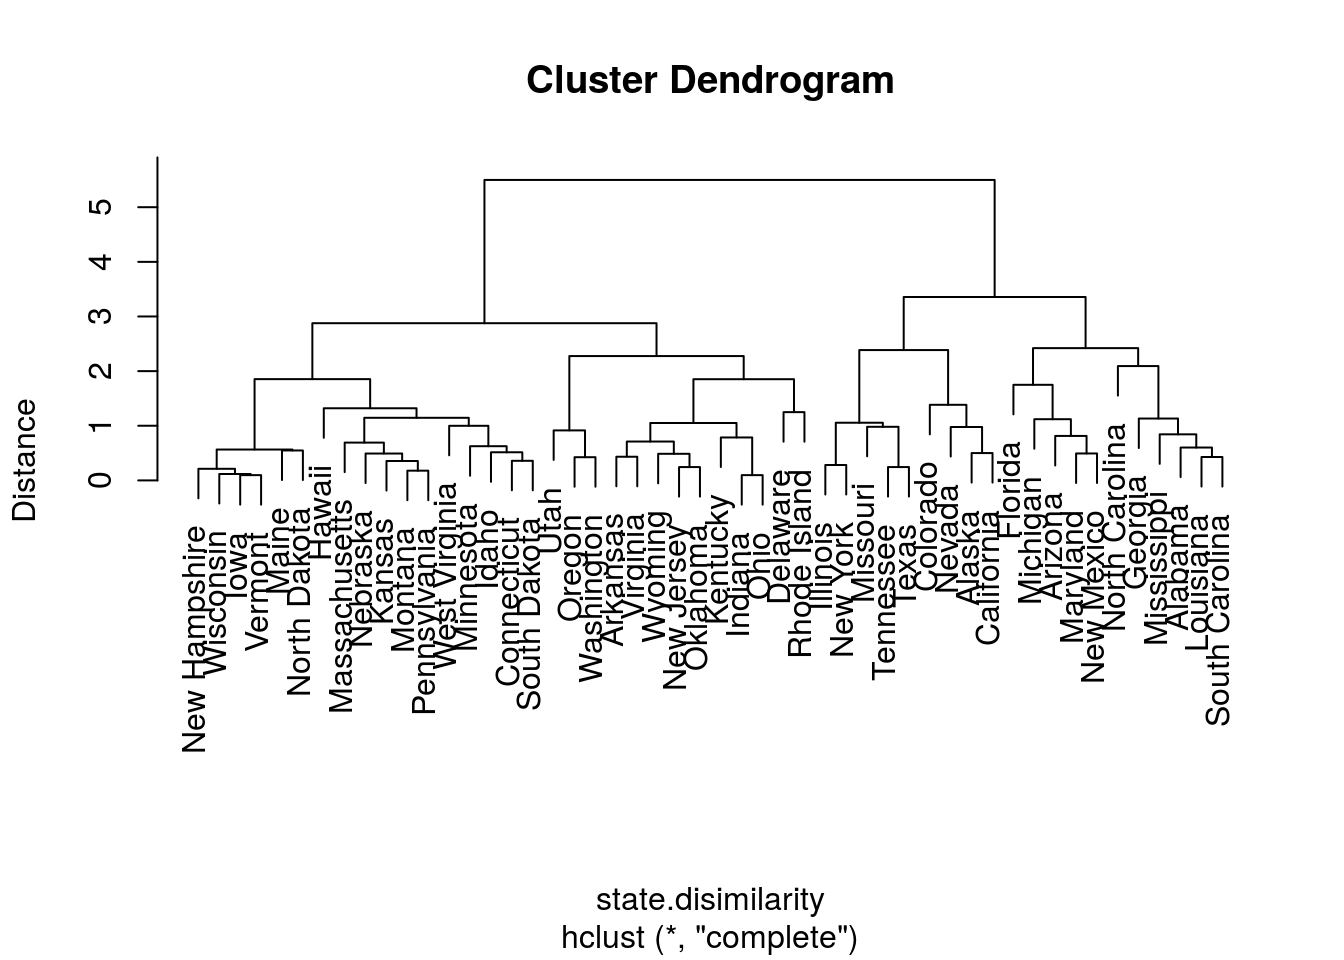
\includegraphics[width=0.5\linewidth]{Rcourse_files/figure-latex/unnamed-chunk-168-1}

Control the line's type with \texttt{lty} argument, and width with
\texttt{lwd}.

\begin{Shaded}
\begin{Highlighting}[]
\KeywordTok{par}\NormalTok{(}\DataTypeTok{mfrow=}\KeywordTok{c}\NormalTok{(}\DecValTok{2}\NormalTok{,}\DecValTok{3}\NormalTok{))}
\KeywordTok{plot}\NormalTok{(Girth, }\DataTypeTok{type=}\StringTok{'l'}\NormalTok{, }\DataTypeTok{lty=}\DecValTok{1}\NormalTok{, }\DataTypeTok{lwd=}\DecValTok{2}\NormalTok{)}
\KeywordTok{plot}\NormalTok{(Girth, }\DataTypeTok{type=}\StringTok{'l'}\NormalTok{, }\DataTypeTok{lty=}\DecValTok{2}\NormalTok{, }\DataTypeTok{lwd=}\DecValTok{2}\NormalTok{)}
\KeywordTok{plot}\NormalTok{(Girth, }\DataTypeTok{type=}\StringTok{'l'}\NormalTok{, }\DataTypeTok{lty=}\DecValTok{3}\NormalTok{, }\DataTypeTok{lwd=}\DecValTok{2}\NormalTok{)}
\KeywordTok{plot}\NormalTok{(Girth, }\DataTypeTok{type=}\StringTok{'l'}\NormalTok{, }\DataTypeTok{lty=}\DecValTok{4}\NormalTok{, }\DataTypeTok{lwd=}\DecValTok{2}\NormalTok{)}
\KeywordTok{plot}\NormalTok{(Girth, }\DataTypeTok{type=}\StringTok{'l'}\NormalTok{, }\DataTypeTok{lty=}\DecValTok{5}\NormalTok{, }\DataTypeTok{lwd=}\DecValTok{2}\NormalTok{)}
\KeywordTok{plot}\NormalTok{(Girth, }\DataTypeTok{type=}\StringTok{'l'}\NormalTok{, }\DataTypeTok{lty=}\DecValTok{6}\NormalTok{, }\DataTypeTok{lwd=}\DecValTok{2}\NormalTok{)}
\end{Highlighting}
\end{Shaded}

\includegraphics[width=0.5\linewidth]{Rcourse_files/figure-latex/unnamed-chunk-169-1}

\begin{Shaded}
\begin{Highlighting}[]
\KeywordTok{par}\NormalTok{(}\DataTypeTok{mfrow=}\KeywordTok{c}\NormalTok{(}\DecValTok{1}\NormalTok{,}\DecValTok{1}\NormalTok{))}
\end{Highlighting}
\end{Shaded}

Add line by slope and intercept with \texttt{abline}.

\begin{Shaded}
\begin{Highlighting}[]
\KeywordTok{plot}\NormalTok{(Girth)}
\KeywordTok{abline}\NormalTok{(}\DataTypeTok{v=}\DecValTok{14}\NormalTok{, }\DataTypeTok{col=}\StringTok{'red'}\NormalTok{) }\CommentTok{# vertical line at 14.}
\KeywordTok{abline}\NormalTok{(}\DataTypeTok{h=}\DecValTok{9}\NormalTok{, }\DataTypeTok{lty=}\DecValTok{4}\NormalTok{,}\DataTypeTok{lwd=}\DecValTok{4}\NormalTok{, }\DataTypeTok{col=}\StringTok{'pink'}\NormalTok{) }\CommentTok{# horizontal line at 9.}
\KeywordTok{abline}\NormalTok{(}\DataTypeTok{a =} \DecValTok{0}\NormalTok{, }\DataTypeTok{b=}\DecValTok{1}\NormalTok{) }\CommentTok{# linear line with intercept a=0, and slope b=1.}
\end{Highlighting}
\end{Shaded}

\includegraphics[width=0.5\linewidth]{Rcourse_files/figure-latex/unnamed-chunk-170-1}

\begin{Shaded}
\begin{Highlighting}[]
\KeywordTok{plot}\NormalTok{(Girth)}
\KeywordTok{points}\NormalTok{(}\DataTypeTok{x=}\DecValTok{1}\NormalTok{:}\DecValTok{30}\NormalTok{, }\DataTypeTok{y=}\KeywordTok{rep}\NormalTok{(}\DecValTok{12}\NormalTok{,}\DecValTok{30}\NormalTok{), }\DataTypeTok{cex=}\FloatTok{0.5}\NormalTok{, }\DataTypeTok{col=}\StringTok{'darkblue'}\NormalTok{)}
\KeywordTok{lines}\NormalTok{(}\DataTypeTok{x=}\KeywordTok{rep}\NormalTok{(}\KeywordTok{c}\NormalTok{(}\DecValTok{5}\NormalTok{,}\DecValTok{10}\NormalTok{), }\DecValTok{7}\NormalTok{), }\DataTypeTok{y=}\DecValTok{7}\NormalTok{:}\DecValTok{20}\NormalTok{, }\DataTypeTok{lty=}\DecValTok{2} \NormalTok{)}
\KeywordTok{lines}\NormalTok{(}\DataTypeTok{x=}\KeywordTok{rep}\NormalTok{(}\KeywordTok{c}\NormalTok{(}\DecValTok{5}\NormalTok{,}\DecValTok{10}\NormalTok{), }\DecValTok{7}\NormalTok{)+}\DecValTok{2}\NormalTok{, }\DataTypeTok{y=}\DecValTok{7}\NormalTok{:}\DecValTok{20}\NormalTok{, }\DataTypeTok{lty=}\DecValTok{2} \NormalTok{)}
\KeywordTok{lines}\NormalTok{(}\DataTypeTok{x=}\KeywordTok{rep}\NormalTok{(}\KeywordTok{c}\NormalTok{(}\DecValTok{5}\NormalTok{,}\DecValTok{10}\NormalTok{), }\DecValTok{7}\NormalTok{)+}\DecValTok{4}\NormalTok{, }\DataTypeTok{y=}\DecValTok{7}\NormalTok{:}\DecValTok{20}\NormalTok{, }\DataTypeTok{lty=}\DecValTok{2} \NormalTok{, }\DataTypeTok{col=}\StringTok{'darkgreen'}\NormalTok{)}
\KeywordTok{lines}\NormalTok{(}\DataTypeTok{x=}\KeywordTok{rep}\NormalTok{(}\KeywordTok{c}\NormalTok{(}\DecValTok{5}\NormalTok{,}\DecValTok{10}\NormalTok{), }\DecValTok{7}\NormalTok{)+}\DecValTok{6}\NormalTok{, }\DataTypeTok{y=}\DecValTok{7}\NormalTok{:}\DecValTok{20}\NormalTok{, }\DataTypeTok{lty=}\DecValTok{4} \NormalTok{, }\DataTypeTok{col=}\StringTok{'brown'}\NormalTok{, }\DataTypeTok{lwd=}\DecValTok{4}\NormalTok{)}
\end{Highlighting}
\end{Shaded}

\includegraphics[width=0.5\linewidth]{Rcourse_files/figure-latex/unnamed-chunk-171-1}

Things to note: - \texttt{points} adds points on an existing plot. -
\texttt{lines} adds lines on an existing plot. - \texttt{col} controls
the color of the element. It takes names or numbers as argument. -
\texttt{cex} controls the scale of the element. Defaults to
\texttt{cex=1}.

Add other elements.

\begin{Shaded}
\begin{Highlighting}[]
\KeywordTok{plot}\NormalTok{(Girth)}
\KeywordTok{segments}\NormalTok{(}\DataTypeTok{x0=}\KeywordTok{rep}\NormalTok{(}\KeywordTok{c}\NormalTok{(}\DecValTok{5}\NormalTok{,}\DecValTok{10}\NormalTok{), }\DecValTok{7}\NormalTok{), }\DataTypeTok{y0=}\DecValTok{7}\NormalTok{:}\DecValTok{20}\NormalTok{, }\DataTypeTok{x1=}\KeywordTok{rep}\NormalTok{(}\KeywordTok{c}\NormalTok{(}\DecValTok{5}\NormalTok{,}\DecValTok{10}\NormalTok{), }\DecValTok{7}\NormalTok{)+}\DecValTok{2}\NormalTok{, }\DataTypeTok{y1=}\NormalTok{(}\DecValTok{7}\NormalTok{:}\DecValTok{20}\NormalTok{)+}\DecValTok{2} \NormalTok{)}
\KeywordTok{arrows}\NormalTok{(}\DataTypeTok{x0=}\DecValTok{13}\NormalTok{,}\DataTypeTok{y0=}\DecValTok{16}\NormalTok{,}\DataTypeTok{x1=}\DecValTok{16}\NormalTok{,}\DataTypeTok{y1=}\DecValTok{17}\NormalTok{, )}
\KeywordTok{rect}\NormalTok{(}\DataTypeTok{xleft=}\DecValTok{10}\NormalTok{, }\DataTypeTok{ybottom=}\DecValTok{12}\NormalTok{,  }\DataTypeTok{xright=}\DecValTok{12}\NormalTok{, }\DataTypeTok{ytop=}\DecValTok{16}\NormalTok{)}
\KeywordTok{polygon}\NormalTok{(}\DataTypeTok{x=}\KeywordTok{c}\NormalTok{(}\DecValTok{10}\NormalTok{,}\DecValTok{11}\NormalTok{,}\DecValTok{12}\NormalTok{,}\FloatTok{11.5}\NormalTok{,}\FloatTok{10.5}\NormalTok{), }\DataTypeTok{y=}\KeywordTok{c}\NormalTok{(}\DecValTok{9}\NormalTok{,}\FloatTok{9.5}\NormalTok{,}\DecValTok{10}\NormalTok{,}\FloatTok{10.5}\NormalTok{,}\FloatTok{9.8}\NormalTok{), }\DataTypeTok{col=}\StringTok{'grey'}\NormalTok{)}
\KeywordTok{title}\NormalTok{(}\DataTypeTok{main=}\StringTok{'This plot makes no sense'}\NormalTok{, }\DataTypeTok{sub=}\StringTok{'Or does it?'}\NormalTok{)}
\KeywordTok{mtext}\NormalTok{(}\StringTok{'Printing in the margins'}\NormalTok{, }\DataTypeTok{side=}\DecValTok{2}\NormalTok{)}
\KeywordTok{mtext}\NormalTok{(}\KeywordTok{expression}\NormalTok{(alpha==}\KeywordTok{log}\NormalTok{(f[i])), }\DataTypeTok{side=}\DecValTok{4}\NormalTok{)}
\end{Highlighting}
\end{Shaded}

\includegraphics[width=0.5\linewidth]{Rcourse_files/figure-latex/unnamed-chunk-172-1}

Things to note: - The following functions add the elements they are
names after: \texttt{segments}, \texttt{arrows}, \texttt{rect},
\texttt{polygon}, \texttt{title}. - \texttt{mtext} adds mathematical
text. For more information for mathematical annotation see
\texttt{?plotmath}.

Add a legend.

\begin{Shaded}
\begin{Highlighting}[]
\KeywordTok{plot}\NormalTok{(Girth, }\DataTypeTok{pch=}\StringTok{'G'}\NormalTok{,}\DataTypeTok{ylim=}\KeywordTok{c}\NormalTok{(}\DecValTok{8}\NormalTok{,}\DecValTok{77}\NormalTok{), }\DataTypeTok{xlab=}\StringTok{'Tree number'}\NormalTok{, }\DataTypeTok{ylab=}\StringTok{''}\NormalTok{, }\DataTypeTok{type=}\StringTok{'b'}\NormalTok{, }\DataTypeTok{col=}\StringTok{'blue'}\NormalTok{)}
\KeywordTok{points}\NormalTok{(Volume, }\DataTypeTok{pch=}\StringTok{'V'}\NormalTok{, }\DataTypeTok{type=}\StringTok{'b'}\NormalTok{, }\DataTypeTok{col=}\StringTok{'red'}\NormalTok{)}
\KeywordTok{legend}\NormalTok{(}\DataTypeTok{x=}\DecValTok{2}\NormalTok{, }\DataTypeTok{y=}\DecValTok{70}\NormalTok{, }\DataTypeTok{legend=}\KeywordTok{c}\NormalTok{(}\StringTok{'Girth'}\NormalTok{, }\StringTok{'Volume'}\NormalTok{), }\DataTypeTok{pch=}\KeywordTok{c}\NormalTok{(}\StringTok{'G'}\NormalTok{,}\StringTok{'V'}\NormalTok{), }\DataTypeTok{col=}\KeywordTok{c}\NormalTok{(}\StringTok{'blue'}\NormalTok{,}\StringTok{'red'}\NormalTok{), }\DataTypeTok{bg=}\StringTok{'grey'}\NormalTok{)}
\end{Highlighting}
\end{Shaded}

\includegraphics[width=0.5\linewidth]{Rcourse_files/figure-latex/unnamed-chunk-173-1}

Adjusting Axes with \texttt{xlim} and \texttt{ylim}.

\begin{Shaded}
\begin{Highlighting}[]
\KeywordTok{plot}\NormalTok{(Girth, }\DataTypeTok{xlim=}\KeywordTok{c}\NormalTok{(}\DecValTok{0}\NormalTok{,}\DecValTok{15}\NormalTok{), }\DataTypeTok{ylim=}\KeywordTok{c}\NormalTok{(}\DecValTok{8}\NormalTok{,}\DecValTok{12}\NormalTok{))}
\end{Highlighting}
\end{Shaded}

\includegraphics[width=0.5\linewidth]{Rcourse_files/figure-latex/unnamed-chunk-174-1}

Use \texttt{layout} for complicated plot layouts.

\begin{Shaded}
\begin{Highlighting}[]
\NormalTok{A<-}\KeywordTok{matrix}\NormalTok{(}\KeywordTok{c}\NormalTok{(}\DecValTok{1}\NormalTok{,}\DecValTok{1}\NormalTok{,}\DecValTok{2}\NormalTok{,}\DecValTok{3}\NormalTok{,}\DecValTok{4}\NormalTok{,}\DecValTok{4}\NormalTok{,}\DecValTok{5}\NormalTok{,}\DecValTok{6}\NormalTok{), }\DataTypeTok{byrow=}\OtherTok{TRUE}\NormalTok{, }\DataTypeTok{ncol=}\DecValTok{2}\NormalTok{)}
\KeywordTok{layout}\NormalTok{(A,}\DataTypeTok{heights=}\KeywordTok{c}\NormalTok{(}\DecValTok{1}\NormalTok{/}\DecValTok{14}\NormalTok{,}\DecValTok{6}\NormalTok{/}\DecValTok{14}\NormalTok{,}\DecValTok{1}\NormalTok{/}\DecValTok{14}\NormalTok{,}\DecValTok{6}\NormalTok{/}\DecValTok{14}\NormalTok{))}

\NormalTok{oma.saved <-}\StringTok{ }\KeywordTok{par}\NormalTok{(}\StringTok{"oma"}\NormalTok{)}
\KeywordTok{par}\NormalTok{(}\DataTypeTok{oma =} \KeywordTok{rep.int}\NormalTok{(}\DecValTok{0}\NormalTok{, }\DecValTok{4}\NormalTok{))}
\KeywordTok{par}\NormalTok{(}\DataTypeTok{oma =} \NormalTok{oma.saved)}
\NormalTok{o.par <-}\StringTok{ }\KeywordTok{par}\NormalTok{(}\DataTypeTok{mar =} \KeywordTok{rep.int}\NormalTok{(}\DecValTok{0}\NormalTok{, }\DecValTok{4}\NormalTok{))}
\NormalTok{for (i in }\KeywordTok{seq_len}\NormalTok{(}\DecValTok{6}\NormalTok{)) \{}
    \KeywordTok{plot.new}\NormalTok{()}
    \KeywordTok{box}\NormalTok{()}
    \KeywordTok{text}\NormalTok{(}\FloatTok{0.5}\NormalTok{, }\FloatTok{0.5}\NormalTok{, }\KeywordTok{paste}\NormalTok{(}\StringTok{'Box no.'}\NormalTok{,i), }\DataTypeTok{cex=}\DecValTok{3}\NormalTok{)}
\NormalTok{\}}
\end{Highlighting}
\end{Shaded}

\includegraphics[width=0.5\linewidth]{Rcourse_files/figure-latex/unnamed-chunk-175-1}

Always detach.

\begin{Shaded}
\begin{Highlighting}[]
\KeywordTok{detach}\NormalTok{(trees)}
\end{Highlighting}
\end{Shaded}

\subsection{The Power of the graphics
device}\label{the-power-of-the-graphics-device}

Building a line graph from scratch.

\begin{Shaded}
\begin{Highlighting}[]
\NormalTok{x =}\StringTok{ }\DecValTok{1995}\NormalTok{:}\DecValTok{2005}
\NormalTok{y =}\StringTok{ }\KeywordTok{c}\NormalTok{(}\FloatTok{81.1}\NormalTok{, }\FloatTok{83.1}\NormalTok{, }\FloatTok{84.3}\NormalTok{, }\FloatTok{85.2}\NormalTok{, }\FloatTok{85.4}\NormalTok{, }\FloatTok{86.5}\NormalTok{, }\FloatTok{88.3}\NormalTok{, }\FloatTok{88.6}\NormalTok{, }\FloatTok{90.8}\NormalTok{, }\FloatTok{91.1}\NormalTok{, }\FloatTok{91.3}\NormalTok{)}
\KeywordTok{plot.new}\NormalTok{()}
\KeywordTok{plot.window}\NormalTok{(}\DataTypeTok{xlim =} \KeywordTok{range}\NormalTok{(x), }\DataTypeTok{ylim =} \KeywordTok{range}\NormalTok{(y))}
\KeywordTok{abline}\NormalTok{(}\DataTypeTok{h =} \NormalTok{-}\DecValTok{4}\NormalTok{:}\DecValTok{4}\NormalTok{, }\DataTypeTok{v =} \NormalTok{-}\DecValTok{4}\NormalTok{:}\DecValTok{4}\NormalTok{, }\DataTypeTok{col =} \StringTok{"lightgrey"}\NormalTok{)}
\KeywordTok{lines}\NormalTok{(x, y, }\DataTypeTok{lwd =} \DecValTok{2}\NormalTok{)}
\KeywordTok{title}\NormalTok{(}\DataTypeTok{main =} \StringTok{"A Line Graph Example"}\NormalTok{,}
        \DataTypeTok{xlab =} \StringTok{"Time"}\NormalTok{,}
        \DataTypeTok{ylab =} \StringTok{"Quality of R Graphics"}\NormalTok{)}
\KeywordTok{axis}\NormalTok{(}\DecValTok{1}\NormalTok{)}
\KeywordTok{axis}\NormalTok{(}\DecValTok{2}\NormalTok{)}
\KeywordTok{box}\NormalTok{()}
\end{Highlighting}
\end{Shaded}

\includegraphics[width=0.5\linewidth]{Rcourse_files/figure-latex/unnamed-chunk-177-1}

Things to note:

\begin{itemize}
\tightlist
\item
  \texttt{plot.new} creates a new, empty, plotting device.
\item
  \texttt{plot.window} determines the limits of the plotting region.
\item
  \texttt{axis} adds the axes, and \texttt{box} the framing box.
\item
  The rest of the elements, you already know.
\end{itemize}

Rosette.

\begin{Shaded}
\begin{Highlighting}[]
\NormalTok{n =}\StringTok{ }\DecValTok{17}
\NormalTok{theta =}\StringTok{ }\KeywordTok{seq}\NormalTok{(}\DecValTok{0}\NormalTok{, }\DecValTok{2} \NormalTok{*}\StringTok{ }\NormalTok{pi, }\DataTypeTok{length =} \NormalTok{n +}\StringTok{ }\DecValTok{1}\NormalTok{)[}\DecValTok{1}\NormalTok{:n]}
\NormalTok{x =}\StringTok{ }\KeywordTok{sin}\NormalTok{(theta)}
\NormalTok{y =}\StringTok{ }\KeywordTok{cos}\NormalTok{(theta)}
\NormalTok{v1 =}\StringTok{ }\KeywordTok{rep}\NormalTok{(}\DecValTok{1}\NormalTok{:n, n)}
\NormalTok{v2 =}\StringTok{ }\KeywordTok{rep}\NormalTok{(}\DecValTok{1}\NormalTok{:n, }\KeywordTok{rep}\NormalTok{(n, n))}
\KeywordTok{plot.new}\NormalTok{()}
\KeywordTok{plot.window}\NormalTok{(}\DataTypeTok{xlim =} \KeywordTok{c}\NormalTok{(-}\DecValTok{1}\NormalTok{, }\DecValTok{1}\NormalTok{), }\DataTypeTok{ylim =} \KeywordTok{c}\NormalTok{(-}\DecValTok{1}\NormalTok{, }\DecValTok{1}\NormalTok{), }\DataTypeTok{asp =} \DecValTok{1}\NormalTok{)}
\KeywordTok{segments}\NormalTok{(x[v1], y[v1], x[v2], y[v2])}
\KeywordTok{box}\NormalTok{()}
\end{Highlighting}
\end{Shaded}

\includegraphics[width=0.5\linewidth]{Rcourse_files/figure-latex/unnamed-chunk-178-1}

Arrows.

\begin{Shaded}
\begin{Highlighting}[]
\KeywordTok{plot.new}\NormalTok{()}
\KeywordTok{plot.window}\NormalTok{(}\DataTypeTok{xlim =} \KeywordTok{c}\NormalTok{(}\DecValTok{0}\NormalTok{, }\DecValTok{1}\NormalTok{), }\DataTypeTok{ylim =} \KeywordTok{c}\NormalTok{(}\DecValTok{0}\NormalTok{, }\DecValTok{1}\NormalTok{))}
\KeywordTok{arrows}\NormalTok{(.}\DecValTok{05}\NormalTok{, .}\DecValTok{075}\NormalTok{, .}\DecValTok{45}\NormalTok{, .}\DecValTok{9}\NormalTok{, }\DataTypeTok{code =} \DecValTok{1}\NormalTok{)}
\KeywordTok{arrows}\NormalTok{(.}\DecValTok{55}\NormalTok{, .}\DecValTok{9}\NormalTok{, .}\DecValTok{95}\NormalTok{, .}\DecValTok{075}\NormalTok{, }\DataTypeTok{code =} \DecValTok{2}\NormalTok{)}
\KeywordTok{arrows}\NormalTok{(.}\DecValTok{1}\NormalTok{, }\DecValTok{0}\NormalTok{, .}\DecValTok{9}\NormalTok{, }\DecValTok{0}\NormalTok{, }\DataTypeTok{code =} \DecValTok{3}\NormalTok{)}
\KeywordTok{text}\NormalTok{(.}\DecValTok{5}\NormalTok{, }\DecValTok{1}\NormalTok{, }\StringTok{"A"}\NormalTok{, }\DataTypeTok{cex =} \FloatTok{1.5}\NormalTok{)}
\KeywordTok{text}\NormalTok{(}\DecValTok{0}\NormalTok{, }\DecValTok{0}\NormalTok{, }\StringTok{"B"}\NormalTok{, }\DataTypeTok{cex =} \FloatTok{1.5}\NormalTok{)}
\KeywordTok{text}\NormalTok{(}\DecValTok{1}\NormalTok{, }\DecValTok{0}\NormalTok{, }\StringTok{"C"}\NormalTok{, }\DataTypeTok{cex =} \FloatTok{1.5}\NormalTok{)}
\end{Highlighting}
\end{Shaded}

\includegraphics[width=0.5\linewidth]{Rcourse_files/figure-latex/unnamed-chunk-179-1}

Arrows as error bars.

\begin{Shaded}
\begin{Highlighting}[]
\NormalTok{x =}\StringTok{ }\DecValTok{1}\NormalTok{:}\DecValTok{10}
\NormalTok{y =}\StringTok{ }\KeywordTok{runif}\NormalTok{(}\DecValTok{10}\NormalTok{) +}\StringTok{ }\KeywordTok{rep}\NormalTok{(}\KeywordTok{c}\NormalTok{(}\DecValTok{5}\NormalTok{, }\FloatTok{6.5}\NormalTok{), }\KeywordTok{c}\NormalTok{(}\DecValTok{5}\NormalTok{, }\DecValTok{5}\NormalTok{))}
\NormalTok{yl =}\StringTok{ }\NormalTok{y -}\StringTok{ }\FloatTok{0.25} \NormalTok{-}\StringTok{ }\KeywordTok{runif}\NormalTok{(}\DecValTok{10}\NormalTok{)/}\DecValTok{3}
\NormalTok{yu =}\StringTok{ }\NormalTok{y +}\StringTok{ }\FloatTok{0.25} \NormalTok{+}\StringTok{ }\KeywordTok{runif}\NormalTok{(}\DecValTok{10}\NormalTok{)/}\DecValTok{3}
\KeywordTok{plot.new}\NormalTok{()}
\KeywordTok{plot.window}\NormalTok{(}\DataTypeTok{xlim =} \KeywordTok{c}\NormalTok{(}\FloatTok{0.5}\NormalTok{, }\FloatTok{10.5}\NormalTok{), }\DataTypeTok{ylim =} \KeywordTok{range}\NormalTok{(yl, yu))}
\KeywordTok{arrows}\NormalTok{(x, yl, x, yu, }\DataTypeTok{code =} \DecValTok{3}\NormalTok{, }\DataTypeTok{angle =} \DecValTok{90}\NormalTok{, }\DataTypeTok{length =} \NormalTok{.}\DecValTok{125}\NormalTok{)}
\KeywordTok{points}\NormalTok{(x, y, }\DataTypeTok{pch =} \DecValTok{19}\NormalTok{, }\DataTypeTok{cex =} \FloatTok{1.5}\NormalTok{)}
\KeywordTok{axis}\NormalTok{(}\DecValTok{1}\NormalTok{, }\DataTypeTok{at =} \DecValTok{1}\NormalTok{:}\DecValTok{10}\NormalTok{, }\DataTypeTok{labels =} \NormalTok{LETTERS[}\DecValTok{1}\NormalTok{:}\DecValTok{10}\NormalTok{])}
\KeywordTok{axis}\NormalTok{(}\DecValTok{2}\NormalTok{, }\DataTypeTok{las =} \DecValTok{1}\NormalTok{)}
\KeywordTok{box}\NormalTok{()}
\end{Highlighting}
\end{Shaded}

\includegraphics[width=0.5\linewidth]{Rcourse_files/figure-latex/unnamed-chunk-180-1}

A histogram is nothing but a bunch of rectangle elements.

\begin{Shaded}
\begin{Highlighting}[]
\KeywordTok{plot.new}\NormalTok{()}
\KeywordTok{plot.window}\NormalTok{(}\DataTypeTok{xlim =} \KeywordTok{c}\NormalTok{(}\DecValTok{0}\NormalTok{, }\DecValTok{5}\NormalTok{), }\DataTypeTok{ylim =} \KeywordTok{c}\NormalTok{(}\DecValTok{0}\NormalTok{, }\DecValTok{10}\NormalTok{))}
\KeywordTok{rect}\NormalTok{(}\DecValTok{0}\NormalTok{:}\DecValTok{4}\NormalTok{, }\DecValTok{0}\NormalTok{, }\DecValTok{1}\NormalTok{:}\DecValTok{5}\NormalTok{, }\KeywordTok{c}\NormalTok{(}\DecValTok{7}\NormalTok{, }\DecValTok{8}\NormalTok{, }\DecValTok{4}\NormalTok{, }\DecValTok{3}\NormalTok{), }\DataTypeTok{col =} \StringTok{"lightblue"}\NormalTok{)}
\KeywordTok{axis}\NormalTok{(}\DecValTok{1}\NormalTok{)}
\KeywordTok{axis}\NormalTok{(}\DecValTok{2}\NormalTok{, }\DataTypeTok{las =} \DecValTok{1}\NormalTok{)}
\end{Highlighting}
\end{Shaded}

\includegraphics[width=0.5\linewidth]{Rcourse_files/figure-latex/unnamed-chunk-181-1}

Spiral Squares.

\begin{Shaded}
\begin{Highlighting}[]
\KeywordTok{plot.new}\NormalTok{()}
\KeywordTok{plot.window}\NormalTok{(}\DataTypeTok{xlim =} \KeywordTok{c}\NormalTok{(-}\DecValTok{1}\NormalTok{, }\DecValTok{1}\NormalTok{), }\DataTypeTok{ylim =} \KeywordTok{c}\NormalTok{(-}\DecValTok{1}\NormalTok{, }\DecValTok{1}\NormalTok{), }\DataTypeTok{asp =} \DecValTok{1}\NormalTok{)}
\NormalTok{x =}\StringTok{ }\KeywordTok{c}\NormalTok{(-}\DecValTok{1}\NormalTok{, }\DecValTok{1}\NormalTok{, }\DecValTok{1}\NormalTok{, -}\DecValTok{1}\NormalTok{)}
\NormalTok{y =}\StringTok{ }\KeywordTok{c}\NormalTok{( }\DecValTok{1}\NormalTok{, }\DecValTok{1}\NormalTok{, -}\DecValTok{1}\NormalTok{, -}\DecValTok{1}\NormalTok{)}
\KeywordTok{polygon}\NormalTok{(x, y, }\DataTypeTok{col =} \StringTok{"cornsilk"}\NormalTok{)}
\NormalTok{vertex1 =}\StringTok{ }\KeywordTok{c}\NormalTok{(}\DecValTok{1}\NormalTok{, }\DecValTok{2}\NormalTok{, }\DecValTok{3}\NormalTok{, }\DecValTok{4}\NormalTok{)}
\NormalTok{vertex2 =}\StringTok{ }\KeywordTok{c}\NormalTok{(}\DecValTok{2}\NormalTok{, }\DecValTok{3}\NormalTok{, }\DecValTok{4}\NormalTok{, }\DecValTok{1}\NormalTok{)}
\NormalTok{for(i in }\DecValTok{1}\NormalTok{:}\DecValTok{50}\NormalTok{) \{}
    \NormalTok{x =}\StringTok{ }\FloatTok{0.9} \NormalTok{*}\StringTok{ }\NormalTok{x[vertex1] +}\StringTok{ }\FloatTok{0.1} \NormalTok{*}\StringTok{ }\NormalTok{x[vertex2]}
    \NormalTok{y =}\StringTok{ }\FloatTok{0.9} \NormalTok{*}\StringTok{ }\NormalTok{y[vertex1] +}\StringTok{ }\FloatTok{0.1} \NormalTok{*}\StringTok{ }\NormalTok{y[vertex2]}
    \KeywordTok{polygon}\NormalTok{(x, y, }\DataTypeTok{col =} \StringTok{"cornsilk"}\NormalTok{)}
\NormalTok{\}}
\end{Highlighting}
\end{Shaded}

\includegraphics[width=0.5\linewidth]{Rcourse_files/figure-latex/unnamed-chunk-182-1}

Circles are just dense polygons.

\begin{Shaded}
\begin{Highlighting}[]
\NormalTok{R =}\StringTok{ }\DecValTok{1}
\NormalTok{xc =}\StringTok{ }\DecValTok{0}
\NormalTok{yc =}\StringTok{ }\DecValTok{0}
\NormalTok{n =}\StringTok{ }\DecValTok{72}
\NormalTok{t =}\StringTok{ }\KeywordTok{seq}\NormalTok{(}\DecValTok{0}\NormalTok{, }\DecValTok{2} \NormalTok{*}\StringTok{ }\NormalTok{pi, }\DataTypeTok{length =} \NormalTok{n)[}\DecValTok{1}\NormalTok{:(n}\DecValTok{-1}\NormalTok{)]}
\NormalTok{x =}\StringTok{ }\NormalTok{xc +}\StringTok{ }\NormalTok{R *}\StringTok{ }\KeywordTok{cos}\NormalTok{(t)}
\NormalTok{y =}\StringTok{ }\NormalTok{yc +}\StringTok{ }\NormalTok{R *}\StringTok{ }\KeywordTok{sin}\NormalTok{(t)}
\KeywordTok{plot.new}\NormalTok{()}
\KeywordTok{plot.window}\NormalTok{(}\DataTypeTok{xlim =} \KeywordTok{range}\NormalTok{(x), }\DataTypeTok{ylim =} \KeywordTok{range}\NormalTok{(y), }\DataTypeTok{asp =} \DecValTok{1}\NormalTok{)}
\KeywordTok{polygon}\NormalTok{(x, y, }\DataTypeTok{col =} \StringTok{"lightblue"}\NormalTok{, }\DataTypeTok{border =} \StringTok{"navyblue"}\NormalTok{)}
\end{Highlighting}
\end{Shaded}

\includegraphics[width=0.5\linewidth]{Rcourse_files/figure-latex/unnamed-chunk-183-1}

Spiral- just a bunch of lines.

\begin{Shaded}
\begin{Highlighting}[]
\NormalTok{k =}\StringTok{ }\DecValTok{5}
\NormalTok{n =}\StringTok{ }\NormalTok{k *}\StringTok{ }\DecValTok{72}
\NormalTok{theta =}\StringTok{ }\KeywordTok{seq}\NormalTok{(}\DecValTok{0}\NormalTok{, k *}\StringTok{ }\DecValTok{2} \NormalTok{*}\StringTok{ }\NormalTok{pi, }\DataTypeTok{length =} \NormalTok{n)}
\NormalTok{R =}\StringTok{ }\NormalTok{.}\DecValTok{98}\NormalTok{^(}\DecValTok{1}\NormalTok{:n -}\StringTok{ }\DecValTok{1}\NormalTok{)}
\NormalTok{x =}\StringTok{ }\NormalTok{R *}\StringTok{ }\KeywordTok{cos}\NormalTok{(theta)}
\NormalTok{y =}\StringTok{ }\NormalTok{R *}\StringTok{ }\KeywordTok{sin}\NormalTok{(theta)}
\KeywordTok{plot.new}\NormalTok{()}
\KeywordTok{plot.window}\NormalTok{(}\DataTypeTok{xlim =} \KeywordTok{range}\NormalTok{(x), }\DataTypeTok{ylim =} \KeywordTok{range}\NormalTok{(y), }\DataTypeTok{asp =} \DecValTok{1}\NormalTok{)}
\KeywordTok{lines}\NormalTok{(x, y)}
\end{Highlighting}
\end{Shaded}

\includegraphics[width=0.5\linewidth]{Rcourse_files/figure-latex/unnamed-chunk-184-1}

\subsection{Exporting a Plot}\label{exporting-a-plot}

The pipeline for exporting graphics is similar to the export of data.
Instead of the \texttt{write.table} or \texttt{save} functions, we will
use the \texttt{pdf}, \texttt{tiff}, \texttt{png}, functions. Depending
on the type of desired output.

Check and set the working directory.

\begin{Shaded}
\begin{Highlighting}[]
\KeywordTok{getwd}\NormalTok{()}
\KeywordTok{setwd}\NormalTok{(}\StringTok{"/tmp/"}\NormalTok{)}
\end{Highlighting}
\end{Shaded}

Export tiff.

\begin{Shaded}
\begin{Highlighting}[]
\KeywordTok{tiff}\NormalTok{(}\DataTypeTok{filename=}\StringTok{'graphicExample.tiff'}\NormalTok{)}
\KeywordTok{plot}\NormalTok{(}\KeywordTok{rnorm}\NormalTok{(}\DecValTok{100}\NormalTok{))}
\KeywordTok{dev.off}\NormalTok{()}
\end{Highlighting}
\end{Shaded}

Things to note:

\begin{itemize}
\tightlist
\item
  The \texttt{tiff} function tells R to open a .tiff file, and write the
  output of a plot.
\item
  Only a single (the last) plot is saved.
\item
  \texttt{dev.off} is close to close the tiff device, and return the
  plotting to the R console (or RStudio).
\end{itemize}

If you want to produce several plots, you can use a counter in the
file's name.

\begin{Shaded}
\begin{Highlighting}[]
\KeywordTok{tiff}\NormalTok{(}\DataTypeTok{filename=}\StringTok{'graphicExample%d.tiff'}\NormalTok{) }\CommentTok{#Creates a sequence of files}
\KeywordTok{plot}\NormalTok{(}\KeywordTok{rnorm}\NormalTok{(}\DecValTok{100}\NormalTok{))}
\KeywordTok{boxplot}\NormalTok{(}\KeywordTok{rnorm}\NormalTok{(}\DecValTok{100}\NormalTok{))}
\KeywordTok{hist}\NormalTok{(}\KeywordTok{rnorm}\NormalTok{(}\DecValTok{100}\NormalTok{))}
\KeywordTok{dev.off}\NormalTok{()}
\end{Highlighting}
\end{Shaded}

\begin{verbatim}
## pdf 
##   2
\end{verbatim}

To see the list of all open devices use \texttt{dev.list()}. To close
\textbf{all} device, (not the last one), use \texttt{graphics.off()}.

See \texttt{?pdf} and \texttt{?jpeg} for more info.

\section{The ggplot2 System}\label{the-ggplot2-system}

The philosophy of \textbf{ggplot2} is very different from the
\textbf{graphics} device. Recall, in \textbf{ggplot2}, a plot is a
object. It can be queryied, it can be changed, and among other things,
it can be plotted.

\textbf{ggplot2} provides a convenience function for many plots:
\texttt{qplot}. We take a non-typical approach by ignoring this
function, and presenting the fundamental building blocks. Once the
building blocks have been understood, mastering \texttt{qplot} will be
easy.

The following is taken from
\href{http://www.ats.ucla.edu/stat/r/seminars/ggplot2_intro/ggplot2_intro.htm}{UCLA's
idre}.

A \textbf{ggplot2} object will have the following elements:

\begin{itemize}
\tightlist
\item
  \textbf{Data} are the variables mapped to aesthetic features of the
  graph.
\item
  \textbf{Aes} is the mapping between objects to their visualization.
\item
  \textbf{Geoms} are the objects/shapes you see on the graph.
\item
  \textbf{Stats} are statistical transformations that summarize data,
  such as the mean or confidence intervals.
\item
  \textbf{Scales} define which aesthetic values are mapped to data
  values. Legends and axes display these mappings.
\item
  \textbf{Coordiante systems} define the plane on which data are mapped
  on the graphic.
\item
  \textbf{Faceting} splits the data into subsets to create multiple
  variations of the same graph (paneling).
\end{itemize}

The \texttt{nlme::Milk} dataset has the protein level of various cows,
at various times, with various diets.

\begin{Shaded}
\begin{Highlighting}[]
\KeywordTok{library}\NormalTok{(nlme)}
\KeywordTok{data}\NormalTok{(Milk)}
\KeywordTok{head}\NormalTok{(Milk)}
\end{Highlighting}
\end{Shaded}

\begin{verbatim}
## Grouped Data: protein ~ Time | Cow
##   protein Time Cow   Diet
## 1    3.63    1 B01 barley
## 2    3.57    2 B01 barley
## 3    3.47    3 B01 barley
## 4    3.65    4 B01 barley
## 5    3.89    5 B01 barley
## 6    3.73    6 B01 barley
\end{verbatim}

\begin{Shaded}
\begin{Highlighting}[]
\KeywordTok{library}\NormalTok{(ggplot2)}
\KeywordTok{ggplot}\NormalTok{(}\DataTypeTok{data =} \NormalTok{Milk, }\KeywordTok{aes}\NormalTok{(}\DataTypeTok{x=}\NormalTok{Time, }\DataTypeTok{y=}\NormalTok{protein)) +}
\StringTok{  }\KeywordTok{geom_point}\NormalTok{()}
\end{Highlighting}
\end{Shaded}

\includegraphics[width=0.5\linewidth]{Rcourse_files/figure-latex/unnamed-chunk-189-1}

Things to note:

\begin{itemize}
\tightlist
\item
  The \texttt{ggplot} function is the constructor of the
  \textbf{ggplot2} object. If the object is not assigned, it is plotted.
\item
  The \texttt{aes} argument tells R that the \texttt{Time} variable in
  the \texttt{Milk} data is the x axis, and protein is y.
\item
  The \texttt{geom\_point} defines the \textbf{Geom}, i.e., it tells R
  to plot the points as they are (and not lines, histograms, etc.).
\item
  The \textbf{ggplot2} object is build by compounding its various
  elements separated by the \texttt{+} operator.
\item
  All the variables that we will need are assumed to be in the
  \texttt{Milk} data frame. This means that (a) the data needs to be a
  data frame (not a matrix for instance), and (b) we will not be able to
  use variables that are not in the \texttt{Milk} data frame.
\end{itemize}

Let's add some color.

\begin{Shaded}
\begin{Highlighting}[]
\KeywordTok{ggplot}\NormalTok{(}\DataTypeTok{data =} \NormalTok{Milk, }\KeywordTok{aes}\NormalTok{(}\DataTypeTok{x=}\NormalTok{Time, }\DataTypeTok{y=}\NormalTok{protein)) +}
\StringTok{  }\KeywordTok{geom_point}\NormalTok{(}\KeywordTok{aes}\NormalTok{(}\DataTypeTok{color=}\NormalTok{Diet))}
\end{Highlighting}
\end{Shaded}

\includegraphics[width=0.5\linewidth]{Rcourse_files/figure-latex/unnamed-chunk-190-1}

The \texttt{color} argument tells R to use the variable \texttt{Diet} as
the coloring. If we wanted a fixed color, and not a variable dependent
color, \texttt{color} would have been put \textbf{outside} the
\texttt{aes} function.

\begin{Shaded}
\begin{Highlighting}[]
\KeywordTok{ggplot}\NormalTok{(}\DataTypeTok{data =} \NormalTok{Milk, }\KeywordTok{aes}\NormalTok{(}\DataTypeTok{x=}\NormalTok{Time, }\DataTypeTok{y=}\NormalTok{protein)) +}
\StringTok{  }\KeywordTok{geom_point}\NormalTok{(}\DataTypeTok{color=}\StringTok{"green"}\NormalTok{)}
\end{Highlighting}
\end{Shaded}

\includegraphics[width=0.5\linewidth]{Rcourse_files/figure-latex/unnamed-chunk-191-1}

Let's save the \textbf{ggplot2} object so we can reuse it. Notice it is
not plotted.

\begin{Shaded}
\begin{Highlighting}[]
\NormalTok{p <-}\StringTok{ }\KeywordTok{ggplot}\NormalTok{(}\DataTypeTok{data =} \NormalTok{Milk, }\KeywordTok{aes}\NormalTok{(}\DataTypeTok{x=}\NormalTok{Time, }\DataTypeTok{y=}\NormalTok{protein)) +}
\StringTok{  }\KeywordTok{geom_point}\NormalTok{()}
\end{Highlighting}
\end{Shaded}

We can add \textbf{layers} using the \texttt{+} operator. Here, we add a
smoothing line.

\begin{Shaded}
\begin{Highlighting}[]
\NormalTok{p +}\StringTok{ }\KeywordTok{geom_smooth}\NormalTok{()}
\end{Highlighting}
\end{Shaded}

\begin{verbatim}
## `geom_smooth()` using method = 'gam'
\end{verbatim}

\includegraphics[width=0.5\linewidth]{Rcourse_files/figure-latex/unnamed-chunk-193-1}

Things to note:

\begin{itemize}
\tightlist
\item
  The smoothing line is a layer added with the \texttt{geom\_smooth()}
  function.
\item
  Lacking any arguments, the new layer will inherit the \texttt{aes} of
  the original object, x and y variables in particular.
\end{itemize}

To split the plot along some variable, we use faceting, done with the
\texttt{facet\_wrap} function.

\begin{Shaded}
\begin{Highlighting}[]
\NormalTok{p +}\StringTok{ }\KeywordTok{facet_wrap}\NormalTok{(~Diet)}
\end{Highlighting}
\end{Shaded}

\includegraphics[width=0.5\linewidth]{Rcourse_files/figure-latex/unnamed-chunk-194-1}

We now add a layer of the mean of each \texttt{Diet} subgroup, connected
by lines.

\begin{Shaded}
\begin{Highlighting}[]
\NormalTok{p +}\StringTok{ }\KeywordTok{stat_summary}\NormalTok{(}\KeywordTok{aes}\NormalTok{(}\DataTypeTok{color=}\NormalTok{Diet), }\DataTypeTok{fun.y=}\StringTok{"mean"}\NormalTok{, }\DataTypeTok{geom=}\StringTok{"line"}\NormalTok{)}
\end{Highlighting}
\end{Shaded}

\includegraphics[width=0.5\linewidth]{Rcourse_files/figure-latex/unnamed-chunk-195-1}

Things to note:

\begin{itemize}
\tightlist
\item
  \texttt{stat\_summary} adds a statistical summary.
\item
  The summary is applied along \texttt{Diet} subgroups, because of the
  \texttt{color=Diet} aesthetic.
\item
  The summary to be applied is the mean, because of
  \texttt{fun.y="mean"}.
\item
  The group means are connected by lines, because of the
  \texttt{geom="line"} argument.
\end{itemize}

What layers can be added using the \textbf{geoms} family of functions?

\begin{itemize}
\tightlist
\item
  \textbf{geom\_bar}: bars with bases on the x-axis.
\item
  \textbf{geom\_boxplot}: boxes-and-whiskers.
\item
  \textbf{geom\_errorbar}: T-shaped error bars.
\item
  \textbf{geom\_histogram}: histogram.
\item
  \textbf{geom\_line}: lines.
\item
  \textbf{geom\_point}: points (scatterplot).
\item
  \textbf{geom\_ribbon}: bands spanning y-values across a range of
  x-values.
\item
  \textbf{geom\_smooth}: smoothed conditional means (e.g.~loess smooth).
\end{itemize}

To demonstrate the layers added with the \textbf{geoms} functions, we
start with a histogram.

\begin{Shaded}
\begin{Highlighting}[]
\NormalTok{pro <-}\StringTok{ }\KeywordTok{ggplot}\NormalTok{(Milk, }\KeywordTok{aes}\NormalTok{(}\DataTypeTok{x=}\NormalTok{protein))}
\NormalTok{pro +}\StringTok{ }\KeywordTok{geom_histogram}\NormalTok{()}
\end{Highlighting}
\end{Shaded}

\begin{verbatim}
## `stat_bin()` using `bins = 30`. Pick better value with `binwidth`.
\end{verbatim}

\includegraphics[width=0.5\linewidth]{Rcourse_files/figure-latex/unnamed-chunk-196-1}

A bar plot.

\begin{Shaded}
\begin{Highlighting}[]
\KeywordTok{ggplot}\NormalTok{(Milk, }\KeywordTok{aes}\NormalTok{(}\DataTypeTok{x=}\NormalTok{Diet)) +}
\StringTok{  }\KeywordTok{geom_bar}\NormalTok{()}
\end{Highlighting}
\end{Shaded}

\includegraphics[width=0.5\linewidth]{Rcourse_files/figure-latex/unnamed-chunk-197-1}

A scatter plot.

\begin{Shaded}
\begin{Highlighting}[]
\NormalTok{tp <-}\StringTok{ }\KeywordTok{ggplot}\NormalTok{(Milk, }\KeywordTok{aes}\NormalTok{(}\DataTypeTok{x=}\NormalTok{Time, }\DataTypeTok{y=}\NormalTok{protein))}
\NormalTok{tp +}\StringTok{ }\KeywordTok{geom_point}\NormalTok{()}
\end{Highlighting}
\end{Shaded}

\includegraphics[width=0.5\linewidth]{Rcourse_files/figure-latex/unnamed-chunk-198-1}

A smooth regression plot, reusing the \texttt{tp} object.

\begin{Shaded}
\begin{Highlighting}[]
\NormalTok{tp +}\StringTok{ }\KeywordTok{geom_smooth}\NormalTok{()}
\end{Highlighting}
\end{Shaded}

\begin{verbatim}
## `geom_smooth()` using method = 'gam'
\end{verbatim}

\includegraphics[width=0.5\linewidth]{Rcourse_files/figure-latex/unnamed-chunk-199-1}

And now, a simple line plot, reusing the \texttt{tp} object, and
connecting lines along \texttt{Cow}.

\begin{Shaded}
\begin{Highlighting}[]
\NormalTok{tp +}\StringTok{ }\KeywordTok{geom_line}\NormalTok{(}\KeywordTok{aes}\NormalTok{(}\DataTypeTok{group=}\NormalTok{Cow))}
\end{Highlighting}
\end{Shaded}

\includegraphics[width=0.5\linewidth]{Rcourse_files/figure-latex/unnamed-chunk-200-1}

The line plot is completely incomprehensible. Better look at boxplots
along time (even if committing the \texttt{Cow} information).

\begin{Shaded}
\begin{Highlighting}[]
\NormalTok{tp +}\StringTok{ }\KeywordTok{geom_boxplot}\NormalTok{(}\KeywordTok{aes}\NormalTok{(}\DataTypeTok{group=}\NormalTok{Time))}
\end{Highlighting}
\end{Shaded}

\includegraphics[width=0.5\linewidth]{Rcourse_files/figure-latex/unnamed-chunk-201-1}

We can do some statistics for each subgroup. The following will compute
the mean and standard errors (default of \texttt{stat\_summary}) of
\texttt{protein} at each time point.

\begin{Shaded}
\begin{Highlighting}[]
\KeywordTok{ggplot}\NormalTok{(Milk, }\KeywordTok{aes}\NormalTok{(}\DataTypeTok{x=}\NormalTok{Time, }\DataTypeTok{y=}\NormalTok{protein)) +}
\StringTok{  }\KeywordTok{stat_summary}\NormalTok{()}
\end{Highlighting}
\end{Shaded}

\begin{verbatim}
## No summary function supplied, defaulting to `mean_se()
\end{verbatim}

\includegraphics[width=0.5\linewidth]{Rcourse_files/figure-latex/unnamed-chunk-202-1}

Some popular statistical summaries, have gained their own functions:

\begin{itemize}
\tightlist
\item
  \texttt{mean\_cl\_boot}: mean and bootstrapped confidence interval
  (default 95\%).
\item
  \texttt{mean\_cl\_normal}: mean and Gaussian (t-distribution based)
  confidence interval (default 95\%).
\item
  \texttt{mean\_dsl}: mean plus or minus standard deviation times some
  constant (default constant=2).
\item
  \texttt{median\_hilow}: median and outer quantiles (default outer
  quantiles = 0.025 and 0.975).
\end{itemize}

For less popular statistical summaries, we may specify the statistical
function in \texttt{stat\_summary}. The median is a first example.

\begin{Shaded}
\begin{Highlighting}[]
\KeywordTok{ggplot}\NormalTok{(Milk, }\KeywordTok{aes}\NormalTok{(}\DataTypeTok{x=}\NormalTok{Time, }\DataTypeTok{y=}\NormalTok{protein)) +}
\StringTok{  }\KeywordTok{stat_summary}\NormalTok{(}\DataTypeTok{fun.y=}\StringTok{"median"}\NormalTok{, }\DataTypeTok{geom=}\StringTok{"point"}\NormalTok{)}
\end{Highlighting}
\end{Shaded}

\includegraphics[width=0.5\linewidth]{Rcourse_files/figure-latex/unnamed-chunk-203-1}

We can also define our own statistical summaries.

\begin{Shaded}
\begin{Highlighting}[]
\NormalTok{medianlog <-}\StringTok{ }\NormalTok{function(y) \{}\KeywordTok{median}\NormalTok{(}\KeywordTok{log}\NormalTok{(y))\}}
\KeywordTok{ggplot}\NormalTok{(Milk, }\KeywordTok{aes}\NormalTok{(}\DataTypeTok{x=}\NormalTok{Time, }\DataTypeTok{y=}\NormalTok{protein)) +}
\StringTok{  }\KeywordTok{stat_summary}\NormalTok{(}\DataTypeTok{fun.y=}\StringTok{"medianlog"}\NormalTok{, }\DataTypeTok{geom=}\StringTok{"line"}\NormalTok{)}
\end{Highlighting}
\end{Shaded}

\includegraphics[width=0.5\linewidth]{Rcourse_files/figure-latex/unnamed-chunk-204-1}

\textbf{Scales} define the actual mapping of an aesthetics values to
data values.

\begin{Shaded}
\begin{Highlighting}[]
\KeywordTok{ggplot}\NormalTok{(Milk, }\KeywordTok{aes}\NormalTok{(}\DataTypeTok{x=}\NormalTok{protein, }\DataTypeTok{fill=}\NormalTok{Diet)) +}
\StringTok{  }\KeywordTok{geom_density}\NormalTok{(}\DataTypeTok{alpha=}\DecValTok{1}\NormalTok{/}\DecValTok{3}\NormalTok{) +}
\StringTok{  }\KeywordTok{scale_fill_hue}\NormalTok{()}
\end{Highlighting}
\end{Shaded}

\includegraphics[width=0.5\linewidth]{Rcourse_files/figure-latex/unnamed-chunk-205-1}

Things to note:

\begin{itemize}
\tightlist
\item
  The \texttt{geom\_density} function tells R to plot density plots.
\item
  The \texttt{alpha=1/3} parameter controls the transparency. Set to
  \texttt{alpha=1} for opaque, and \texttt{alpha=0} for transparent.
\item
  The \texttt{scale\_fill\_hue} function, which is the default (thus can
  be omitted), tells R how to map factors to colors.
\end{itemize}

Let's change the default color mapping.

\begin{Shaded}
\begin{Highlighting}[]
\KeywordTok{ggplot}\NormalTok{(Milk, }\KeywordTok{aes}\NormalTok{(}\DataTypeTok{x=}\NormalTok{protein, }\DataTypeTok{fill=}\NormalTok{Diet)) +}
\StringTok{  }\KeywordTok{geom_density}\NormalTok{(}\DataTypeTok{alpha=}\DecValTok{1}\NormalTok{/}\DecValTok{3}\NormalTok{) +}
\StringTok{  }\KeywordTok{scale_fill_hue}\NormalTok{(}\DataTypeTok{h.start=}\DecValTok{150}\NormalTok{)}
\end{Highlighting}
\end{Shaded}

\includegraphics[width=0.5\linewidth]{Rcourse_files/figure-latex/unnamed-chunk-206-1}

The legend is controlled with the \texttt{guides} function.

\begin{Shaded}
\begin{Highlighting}[]
\KeywordTok{ggplot}\NormalTok{(Milk, }\KeywordTok{aes}\NormalTok{(}\DataTypeTok{x=}\NormalTok{protein, }\DataTypeTok{fill=}\NormalTok{Diet)) +}
\StringTok{  }\KeywordTok{geom_density}\NormalTok{(}\DataTypeTok{alpha=}\DecValTok{1}\NormalTok{/}\DecValTok{3}\NormalTok{) +}
\StringTok{  }\KeywordTok{guides}\NormalTok{(}\DataTypeTok{fill=}\StringTok{"none"}\NormalTok{)}
\end{Highlighting}
\end{Shaded}

\includegraphics[width=0.5\linewidth]{Rcourse_files/figure-latex/unnamed-chunk-207-1}

\_\_Faceting allows to split the plotting along some variable.
\texttt{face\_wrap} tells R to compute the number of columns and rows of
plots automatically.

\begin{Shaded}
\begin{Highlighting}[]
\KeywordTok{ggplot}\NormalTok{(Milk, }\KeywordTok{aes}\NormalTok{(}\DataTypeTok{x=}\NormalTok{protein, }\DataTypeTok{color=}\NormalTok{Diet)) +}
\StringTok{  }\KeywordTok{geom_density}\NormalTok{() +}
\StringTok{  }\KeywordTok{facet_wrap}\NormalTok{(~Time)}
\end{Highlighting}
\end{Shaded}

\includegraphics[width=0.5\linewidth]{Rcourse_files/figure-latex/unnamed-chunk-208-1}

\texttt{facet\_grid} forces the plot to appear allow rows or columns,
using the \texttt{\textasciitilde{}} syntax.

\begin{Shaded}
\begin{Highlighting}[]
\KeywordTok{ggplot}\NormalTok{(Milk, }\KeywordTok{aes}\NormalTok{(}\DataTypeTok{x=}\NormalTok{Time, }\DataTypeTok{y=}\NormalTok{protein)) +}
\StringTok{  }\KeywordTok{geom_point}\NormalTok{() +}
\StringTok{  }\KeywordTok{facet_grid}\NormalTok{(Diet~.)}
\end{Highlighting}
\end{Shaded}

\includegraphics[width=0.5\linewidth]{Rcourse_files/figure-latex/unnamed-chunk-209-1}

To control the looks of the plot, \textbf{ggplot2} uses \textbf{themes}.

\begin{Shaded}
\begin{Highlighting}[]
\KeywordTok{ggplot}\NormalTok{(Milk, }\KeywordTok{aes}\NormalTok{(}\DataTypeTok{x=}\NormalTok{Time, }\DataTypeTok{y=}\NormalTok{protein)) +}
\StringTok{  }\KeywordTok{geom_point}\NormalTok{() +}
\StringTok{  }\KeywordTok{theme}\NormalTok{(}\DataTypeTok{panel.background=}\KeywordTok{element_rect}\NormalTok{(}\DataTypeTok{fill=}\StringTok{"lightblue"}\NormalTok{))}
\end{Highlighting}
\end{Shaded}

\includegraphics[width=0.5\linewidth]{Rcourse_files/figure-latex/unnamed-chunk-210-1}

\begin{Shaded}
\begin{Highlighting}[]
\KeywordTok{ggplot}\NormalTok{(Milk, }\KeywordTok{aes}\NormalTok{(}\DataTypeTok{x=}\NormalTok{Time, }\DataTypeTok{y=}\NormalTok{protein)) +}
\StringTok{  }\KeywordTok{geom_point}\NormalTok{() +}
\StringTok{  }\KeywordTok{theme}\NormalTok{(}\DataTypeTok{panel.background=}\KeywordTok{element_blank}\NormalTok{(),}
        \DataTypeTok{axis.title.x=}\KeywordTok{element_blank}\NormalTok{())}
\end{Highlighting}
\end{Shaded}

\includegraphics[width=0.5\linewidth]{Rcourse_files/figure-latex/unnamed-chunk-211-1}

Saving plots can be done using the \texttt{pdf} function, but possibly
easier with the \texttt{ggsave} function.

Finally, what every user of \textbf{ggplot2} constantly uses, is the
online documentation at \url{http://docs.ggplot2.org}.

\section{Interactive Graphics}\label{interactive-graphics}

As already mentioned, the recent and dramatic advancement in interactive
visualization was made possible by the advances in web technologies, and
the \href{https://d3js.org/}{D3.JS} JavaScript library in particular.
This is because it allows developers to rely on existing libraries
designed for web browsing. These libraries are more visually pleasing,
and computationally efficient, than anything they could have developed
themselves.

Some noteworthy interactive plotting systems are the following:

\begin{itemize}
\item
  \textbf{plotly}: The \textbf{plotly} package \citep{plotly} uses the
  (brilliant!) visualization framework of the \href{}{Plotly} company to
  provide local, or web-publishable, interactive graphics.
\item
  \textbf{dygraphs}: The \href{http://dygraphs.com/}{dygraphs}
  JavaScript library is intended for interactive visualization of time
  series. The \textbf{dygraphs} R package is an interface allowing the
  plotting of R objects with this library. For more information see
  \href{https://rstudio.github.io/dygraphs/}{here}.
\item
  \textbf{rCharts}: If you like the \textbf{lattice} plotting system,
  the \textbf{rCharts} package will allow you to produce interactive
  plots from R using the \textbf{lattice} syntax. For more information
  see \href{http://rdatascience.io/rCharts/}{here}.
\item
  \textbf{clickme}: Very similar to \textbf{rCharts}.
\item
  \textbf{ggv2}: \href{https://vega.github.io/vega/}{Vega} is a grammar
  for plots, i.e., a syntax that describes a plots elements, along with
  the appropriate JavaScript visualization libraries. \textbf{ggv2} is
  an an experimental package that produces Vega interactive plots from
  R. For more information see
  \href{https://github.com/metagraf/rVega}{here}.
\item
  \textbf{rVega}: Same purpose as \textbf{ggv2}.
\item
  \textbf{googleVis}: TODO
\item
  \textbf{HTML Widgets}: The \textbf{htmlwidgets} package does not
  provide visualization, but rather, it facilitates the creation of new
  interactive visualizations. This is because it handles all the
  technical details that are required to use R output within JavaScript
  visualization libraries.
\end{itemize}

\subsection{Plotly}\label{plotly}

\begin{Shaded}
\begin{Highlighting}[]
\KeywordTok{library}\NormalTok{(plotly)}
\KeywordTok{set.seed}\NormalTok{(}\DecValTok{100}\NormalTok{)}
\NormalTok{d <-}\StringTok{ }\NormalTok{diamonds[}\KeywordTok{sample}\NormalTok{(}\KeywordTok{nrow}\NormalTok{(diamonds), }\DecValTok{1000}\NormalTok{), ]}
\KeywordTok{plot_ly}\NormalTok{(d, }\DataTypeTok{x =} \NormalTok{~carat, }\DataTypeTok{y =} \NormalTok{~price, }\DataTypeTok{color =} \NormalTok{~carat,}
        \DataTypeTok{size =} \NormalTok{~carat, }\DataTypeTok{text =} \NormalTok{~}\KeywordTok{paste}\NormalTok{(}\StringTok{"Clarity: "}\NormalTok{, clarity))}
\end{Highlighting}
\end{Shaded}

\begin{verbatim}
## No trace type specified:
##   Based on info supplied, a 'scatter' trace seems appropriate.
##   Read more about this trace type -> https://plot.ly/r/reference/#scatter
\end{verbatim}

\begin{verbatim}
## No scatter mode specifed:
##   Setting the mode to markers
##   Read more about this attribute -> https://plot.ly/r/reference/#scatter-mode
\end{verbatim}

\includegraphics[width=0.5\linewidth]{Rcourse_files/figure-latex/unnamed-chunk-212-1}

If you are comfortable with \textbf{ggplot2}, you may use the
\textbf{ggplot2} syntax, and export the final result to \textbf{plotly}.

\begin{Shaded}
\begin{Highlighting}[]
\NormalTok{p <-}\StringTok{ }\KeywordTok{ggplot}\NormalTok{(}\DataTypeTok{data =} \NormalTok{d, }\KeywordTok{aes}\NormalTok{(}\DataTypeTok{x =} \NormalTok{carat, }\DataTypeTok{y =} \NormalTok{price)) +}
\StringTok{  }\KeywordTok{geom_point}\NormalTok{(}\KeywordTok{aes}\NormalTok{(}\DataTypeTok{text =} \KeywordTok{paste}\NormalTok{(}\StringTok{"Clarity:"}\NormalTok{, clarity))) +}
\StringTok{  }\KeywordTok{geom_smooth}\NormalTok{(}\KeywordTok{aes}\NormalTok{(}\DataTypeTok{colour =} \NormalTok{cut, }\DataTypeTok{fill =} \NormalTok{cut)) +}\StringTok{ }\KeywordTok{facet_wrap}\NormalTok{(~}\StringTok{ }\NormalTok{cut)}
\end{Highlighting}
\end{Shaded}

\begin{verbatim}
## Warning: Ignoring unknown aesthetics: text
\end{verbatim}

\begin{Shaded}
\begin{Highlighting}[]
\KeywordTok{ggplotly}\NormalTok{(p)}
\end{Highlighting}
\end{Shaded}

\begin{verbatim}
## `geom_smooth()` using method = 'loess'
\end{verbatim}

\includegraphics[width=0.5\linewidth]{Rcourse_files/figure-latex/unnamed-chunk-213-1}

For more on \textbf{plotly} see \url{https://plot.ly/r/}.

\subsection{HTML Widgets}\label{html-widgets}

\section{Bibliographic Notes}\label{bibliographic-notes-8}

For the \textbf{graphics} package, see \citet{Rlanguage}. For
\textbf{ggplot2} see \citet{ggplot2}.

\chapter{Reports}\label{report}

If you ever written a report, you are probably familiar with the process
of preparing your figures in some software, say R, and then copy-pasting
into your text editor, say MS Word. While very popular, this process is
both tedious, and plain painful if your data has changed and you need to
update the report. Wouldn't it be nice if you could produce figures and
numbers from within the text of the report, and everything else would be
automated? It turns out it is possible. There are actually several
systems in R that allow this. We start with a brief review.

\begin{enumerate}
\def\labelenumi{\arabic{enumi}.}
\item
  \textbf{Sweave}: \emph{Latex} is a markup language that compiles to
  \emph{Tex} programs that compile to documents, typically PDFs. If you
  never heard of it, it may be because you were born the the MS
  Windows+MS Word era. You should know, however, that \emph{Latex} was
  there much earlier, when computers were mainframes with text-only
  graphic devices. You should also know that \emph{Latex} is still very
  popular (in some communities) due to its very rich markup syntax, and
  beautiful output. \emph{Sweave} \citep{leisch2002sweave} is a compiler
  for \emph{Latex} that allows you do insert R commands in the
  \emph{Latex} source file, compile it, and get the result as part of
  the outputted PDF. It's name suggests just that: it allows to weave
  S\footnote{Recall, S was the original software from which R evolved.}
  output into the document, thus, Sweave.
\item
  \textbf{knitr}: \emph{Markdown} is a text editing syntax that is aimed
  to be human-readable, but also compilable by a machine. If you ever
  tried to read HTML or Latex source files, you may understand why
  human-readability is a desirable property. There are many
  \emph{markdown} compilers. One of the most popular is \emph{Pandoc},
  written by the Berkeley philosopher(!) Jon MacFarlane. The
  availability of \emph{Pandoc} gave \href{}{Yihui Xie}, a name to
  remember, the idea that it is time for Sweave to evolve. Yihui thus
  wrote \textbf{knitr} \citep{xie2015dynamic}, which allows to write
  human readable text in \emph{Rmarkdown}, a superset of
  \emph{markdown}, compile it with R and the compile it with Pandoc.
  Because Pandoc can compile to PDF, but also to HTML, and DOCX, among
  others, this means that you can write in Rmarkdown, and get output in
  almost all text formats out there.
\item
  \textbf{bookdown}: \textbf{Bookdown} \citep{xie2016bookdown} is an
  evolution of \textbf{knitr}, also written by Yihui Xie, now working
  for RStudio. This book was actually written in \textbf{bookdown}. It
  deals with the particular needs of writing large documents, and cross
  referencing in particular (which is very challenging if you want the
  text to be human readable).
\item
  \textbf{Shiney}: The previous reporting frameworks are static in that
  R ``dumps'' its output and is never queryied again. This does not mean
  that output is static, but only that R is not called. \textbf{Shiny}
  \citep{shiney} is different. Shiny is essentially a framework for
  quick web-development. It includes (i) an abstraction layer that
  specifies the layout of a web-site which is our report, (ii) the
  command to start a web server to deliver the site. For more on Shiny
  see \citet{shiney}.
\end{enumerate}

\section{knitr}\label{knitr}

\subsection{Installation}\label{installation}

To run \textbf{knitr} you will need to install the package.

\begin{Shaded}
\begin{Highlighting}[]
\KeywordTok{install.packages}\NormalTok{(}\StringTok{'knitr'}\NormalTok{)}
\end{Highlighting}
\end{Shaded}

It is also recommended that you use it within RStudio
(version\textgreater{}0.96), where you can easily create a new
\texttt{.Rmd} file.

\subsection{Pandoc Markdown}\label{pandoc-markdown}

Because \textbf{knitr} builds upon \emph{Pandoc markdown}, here is a
simple example of markdown text, to be used in a \texttt{.Rmd} file,
which can be created using the \emph{File-\textgreater{} New File
-\textgreater{} R Markdown} menu of RStudio.

Underscores or asterisks for \texttt{\_italics1\_} and
\texttt{*italics2*} return \emph{italics1} and \emph{italics2}. Double
underscores or asterisks for \texttt{\_\_bold1\_\_} and
\texttt{**bold2**} return \textbf{bold1} and \textbf{bold2}. Subscripts
are enclosed in tildes,
\texttt{like\textasciitilde{}this\textasciitilde{}}
(like\textsubscript{this}), and superscripts are enclosed in carets
\texttt{like\^{}this\^{}} (like\textsuperscript{this}). For
\texttt{verbatim} use ``\texttt{verbatim}''.

For links use \texttt{{[}text{]}(link)}, like
\texttt{{[}my\ site{]}(www.john-ros.com)}. Image is the same as a link,
starting with an exclamation, like this
\texttt{!{[}image\ title{]}(image\ path)}.

An itemized list simply starts with hyphens:

\begin{verbatim}
- bullet
- bullet
    - second level bullet
    - second level bullet
\end{verbatim}

Compiles into:

\begin{itemize}
\tightlist
\item
  bullet
\item
  bullet

  \begin{itemize}
  \tightlist
  \item
    second level bullet
  \item
    second level bullet
  \end{itemize}
\end{itemize}

An enumerated list starts with an arbitrary number:

\begin{verbatim}
1. number
1. number
    1. second level number
    1. second level number
\end{verbatim}

Compiles into:

\begin{enumerate}
\def\labelenumi{\arabic{enumi}.}
\tightlist
\item
  number
\item
  number

  \begin{enumerate}
  \def\labelenumii{\arabic{enumii}.}
  \tightlist
  \item
    second level number
  \item
    second level number
  \end{enumerate}
\end{enumerate}

For more on markdown see
\href{https://bookdown.org/yihui/bookdown/markdown-syntax.html}{here}.

\subsection{Rmarkdown}\label{rmarkdown}

\emph{Rmarkdown}, is an extension of \emph{markdown} due to RStudio,
that allows to incorporate R expressions in the text, that will be
evaluated at the time of compilation, and the output automatically
inserted in the outputted text. The output can be a \texttt{.PDF},
\texttt{.DOCX}, \texttt{.HTML} or others, thanks to the power of
\textbf{pandoc}.

The start of a code chunk is indicated by three backticks and the end of
a code chunk is indicated by three backticks. Here is an example.

\begin{verbatim}
```{r  eval=FALSE}
rnorm(10)
```
\end{verbatim}

This chunk will compile to the following output (after setting
\texttt{eval=FALSE} to \texttt{eval=TRUE}):

\begin{Shaded}
\begin{Highlighting}[]
\KeywordTok{rnorm}\NormalTok{(}\DecValTok{10}\NormalTok{)}
\end{Highlighting}
\end{Shaded}

\begin{verbatim}
##  [1] -1.4462875  0.3158558 -0.3427475 -1.9313531  0.2428210 -0.3627679
##  [7]  2.4327289  0.5920912 -0.5762008  0.4066282
\end{verbatim}

Things to note:

\begin{itemize}
\tightlist
\item
  The evaluated expression is added in a chunk of highlighted text.
\item
  The output is added prefixed with \texttt{\#\#}.
\item
  The \texttt{eval=} argument is not required, since it is set to
  \texttt{eval=TRUE} by default. It does demonstrate how to set the
  options of the code chunk.
\end{itemize}

In the same way, we may add a plot:

\begin{verbatim}
```{r  eval=FALSE}
plot(rnorm(10))
```
\end{verbatim}

which compiles into

\begin{Shaded}
\begin{Highlighting}[]
\KeywordTok{plot}\NormalTok{(}\KeywordTok{rnorm}\NormalTok{(}\DecValTok{10}\NormalTok{))}
\end{Highlighting}
\end{Shaded}

\includegraphics[width=0.5\linewidth]{Rcourse_files/figure-latex/unnamed-chunk-218-1}

You can also call r expressions inline. This is done with a single tick
and the \texttt{r} argument. For instance:

\begin{quote}
\texttt{`r\ rnorm(1)`} is a random Gaussian
\end{quote}

will output

\begin{quote}
0.3378953 is a random Gaussian.
\end{quote}

\subsection{Compiling}\label{compiling}

Once you have your \texttt{.Rmd} file written in RMarkdown,
\textbf{knitr} will take care of the compilation for you. You can call
the \texttt{knitr::knitr} function directly from some \texttt{.R} file,
or more conveniently, use the RStudio (0.96) Knit button above the text
editing window. The location of the output file will be presented in the
console.

\section{bookdown}\label{bookdown}

As previously stated, \textbf{bookdown} is an extension of
\textbf{knitr} intended for documents more complicated than simple
reports-- such as books. Just like \textbf{knitr}, the writing is done
in \textbf{RMarkdown}. Being an extension of \textbf{knitr},
\textbf{bookdown} does allow some markdowns that are not supported by
other compilers. In particular, it has a more powerful cross referencing
system.

\section{Shiny}\label{shiny}

\textbf{Shiny} \citep{shiny} is different than the previous systems,
because it sets up an interactive web-site, and not a static file. The
power of Shiny is that they layout of the web-site, and setting up the
web-server, is made with several simple R commands, with no need for
web-programming. For this purpose, Shiny uses the
\href{http://getbootstrap.com}{Bootstrap} web development technology.
Once you have your app up and running, you can setup your own Shiny
server on the web, or publish it via
\href{https://www.shinyapps.io/}{Shinyapps.io}. The freemium versions of
the service can deal with a small amount of traffic. If you expect a lot
of traffic, you will probably need the paid versions.

\subsection{Installation}\label{installation-1}

To setup your first Shiny app, you will need the \textbf{shiny} package.
You will probably want RStudio, which facilitates the process.

\begin{Shaded}
\begin{Highlighting}[]
\KeywordTok{install.packages}\NormalTok{(}\StringTok{'shiny'}\NormalTok{)}
\end{Highlighting}
\end{Shaded}

Once installed, you can run an example app to get the feel of it.

\begin{Shaded}
\begin{Highlighting}[]
\KeywordTok{library}\NormalTok{(shiny)}
\KeywordTok{runExample}\NormalTok{(}\StringTok{"01_hello"}\NormalTok{)}
\end{Highlighting}
\end{Shaded}

Remember to press the \textbf{Stop} button in RStudio to stop the
web-server, and get back to RStudio.

\subsection{The Basics of Shiny}\label{the-basics-of-shiny}

Every Shiny app has two main building blocks.

\begin{enumerate}
\def\labelenumi{\arabic{enumi}.}
\tightlist
\item
  A user interface, specified via the \texttt{ui.R} file in the app's
  directory.
\item
  A server side, specified via the \texttt{server.R} file, in the app's
  directory.
\end{enumerate}

You can run the app via the \textbf{RunApp} button in the RStudio
interface, of by calling the app's directory with the \texttt{shinyApp}
or \texttt{runApp} functions-- the former designed for single-app
projects, and the latter, for multiple app projects.

\begin{Shaded}
\begin{Highlighting}[]
\NormalTok{shiny::}\KeywordTok{runApp}\NormalTok{(}\StringTok{"my_app"}\NormalTok{)}
\end{Highlighting}
\end{Shaded}

The site's layout, is specified via \emph{layout functions} in the
\texttt{iu.R} file. For instance, the function \texttt{sidebarLayout},
as the name suggest, will create a sidebar. More layouts are detailed in
the \href{http://shiny.rstudio.com/articles/layout-guide.html}{layout
guide}.

The active elements in the UI, that control your report, are known as
\emph{widgets}. Each widget will have a unique \texttt{inputId} so that
it's values can be sent from the UI to the server. More about widgets,
in the
\href{http://shiny.rstudio.com/gallery/widget-gallery.html}{widget
gallery}.

The \texttt{inputId} on the UI are mapped to \texttt{input} arguments on
the server side. The value of the \texttt{mytext} \texttt{inputId} can
be queryied by the server using \texttt{input\$mytext}. These are called
\emph{reactive values}. The way the server ``listens'' to the UI, is
governed by a set of functions that must wrap the \texttt{input} object.
These are the \texttt{observe}, \texttt{reactive}, and
\texttt{reactive*} class of functions.

With \texttt{observe} the server will get triggered when any of the
reactive values change. With \texttt{observeEvent} the server will only
be triggered by specified reactive values. Using \texttt{observe} is
easier, and \texttt{observeEvent} is more prudent programming.

A \texttt{reactive} function is a function that gets triggered when a
reactive element changes. It is defined on the server side, and reside
within an \texttt{observe} function.

We now analyze the \texttt{1\_Hello} app using these ideas. Here is the
\texttt{io.R} file.

\begin{Shaded}
\begin{Highlighting}[]
\KeywordTok{library}\NormalTok{(shiny)}

\KeywordTok{shinyUI}\NormalTok{(}\KeywordTok{fluidPage}\NormalTok{(}

  \KeywordTok{titlePanel}\NormalTok{(}\StringTok{"Hello Shiny!"}\NormalTok{),}

  \KeywordTok{sidebarLayout}\NormalTok{(}
    \KeywordTok{sidebarPanel}\NormalTok{(}
      \KeywordTok{sliderInput}\NormalTok{(}\DataTypeTok{inputId =} \StringTok{"bins"}\NormalTok{,}
                  \DataTypeTok{label =} \StringTok{"Number of bins:"}\NormalTok{, }
                  \DataTypeTok{min =} \DecValTok{1}\NormalTok{,}
                  \DataTypeTok{max =} \DecValTok{50}\NormalTok{,}
                  \DataTypeTok{value =} \DecValTok{30}\NormalTok{)}
    \NormalTok{),}

    \KeywordTok{mainPanel}\NormalTok{(}
      \KeywordTok{plotOutput}\NormalTok{(}\DataTypeTok{outputId =} \StringTok{"distPlot"}\NormalTok{)}
    \NormalTok{)}
  \NormalTok{)}
\NormalTok{))}
\end{Highlighting}
\end{Shaded}

Here is the \texttt{server.R} file:

\begin{Shaded}
\begin{Highlighting}[]
\KeywordTok{library}\NormalTok{(shiny)}

\KeywordTok{shinyServer}\NormalTok{(function(input, output) \{}

  \NormalTok{output$distPlot <-}\StringTok{ }\KeywordTok{renderPlot}\NormalTok{(\{}
    \NormalTok{x    <-}\StringTok{ }\NormalTok{faithful[, }\DecValTok{2}\NormalTok{]  }\CommentTok{# Old Faithful Geyser data}
    \NormalTok{bins <-}\StringTok{ }\KeywordTok{seq}\NormalTok{(}\KeywordTok{min}\NormalTok{(x), }\KeywordTok{max}\NormalTok{(x), }\DataTypeTok{length.out =} \NormalTok{input$bins +}\StringTok{ }\DecValTok{1}\NormalTok{)}

    \KeywordTok{hist}\NormalTok{(x, }\DataTypeTok{breaks =} \NormalTok{bins, }\DataTypeTok{col =} \StringTok{'darkgray'}\NormalTok{, }\DataTypeTok{border =} \StringTok{'white'}\NormalTok{)}
  \NormalTok{\})}
\NormalTok{\})}
\end{Highlighting}
\end{Shaded}

Things to note:

\begin{itemize}
\tightlist
\item
  \texttt{ShinyUI} is a (deprecated) wrapper for the UI.
\item
  \texttt{fluidPage} ensures that the proportions of the elements adapt
  to the window side, thus, are fluid.
\item
  The building blocks of the layout are a title, and the body. The title
  is governed by \texttt{titlePanel}, and the body is governed by
  \texttt{sidebarLayout}. The \texttt{sidebarLayout} includes the
  \texttt{sidebarPanel} to control the sidebar, and the
  \texttt{mainPanel} for the main panel.
\item
  \texttt{sliderInput} calls a widget with a slider. Its
  \texttt{inputId} is \texttt{bins}, which is later used by the server
  within the \texttt{renderPlot} reactive function.
\item
  \texttt{plotOutput} specifies that the content of the
  \texttt{mainPanel} is a plot (\texttt{textOutput} for text). This
  expectation is satisfied on the server side with the
  \texttt{renderPlot} function (\texttt{renderText}).
\item
  \texttt{shinyServer} is a (deprecated) wrapper function for the
  server.
\item
  The server runs a function with an \texttt{input} and an
  \texttt{output}. The elements of \texttt{input} are the
  \texttt{inputId}s from the UI. The elements of the \texttt{output}
  will be called by the UI using their \texttt{outputId}.
\end{itemize}

This is the output.

\begin{Shaded}
\begin{Highlighting}[]
\NormalTok{knitr::}\KeywordTok{include_url}\NormalTok{(}\StringTok{'http://shiny.rstudio.com/gallery/example-01-hello.html'}\NormalTok{)}
\end{Highlighting}
\end{Shaded}

\href{http://shiny.rstudio.com/gallery/example-01-hello.html}{\includegraphics[width=0.5\linewidth]{Rcourse_files/figure-latex/unnamed-chunk-224-1} }

Here is another example, taken from the RStudio
\href{https://github.com/rstudio/shiny-examples/tree/master/006-tabsets}{Shiny
examples}.

\texttt{ui.R}:

\begin{Shaded}
\begin{Highlighting}[]
\KeywordTok{library}\NormalTok{(shiny)}

\KeywordTok{fluidPage}\NormalTok{(}
    
  \KeywordTok{titlePanel}\NormalTok{(}\StringTok{"Tabsets"}\NormalTok{),}
  
  \KeywordTok{sidebarLayout}\NormalTok{(}
    \KeywordTok{sidebarPanel}\NormalTok{(}
      \KeywordTok{radioButtons}\NormalTok{(}\DataTypeTok{inputId =} \StringTok{"dist"}\NormalTok{, }
                   \DataTypeTok{label =} \StringTok{"Distribution type:"}\NormalTok{,}
                   \KeywordTok{c}\NormalTok{(}\StringTok{"Normal"} \NormalTok{=}\StringTok{ "norm"}\NormalTok{,}
                     \StringTok{"Uniform"} \NormalTok{=}\StringTok{ "unif"}\NormalTok{,}
                     \StringTok{"Log-normal"} \NormalTok{=}\StringTok{ "lnorm"}\NormalTok{,}
                     \StringTok{"Exponential"} \NormalTok{=}\StringTok{ "exp"}\NormalTok{)),}
      \KeywordTok{br}\NormalTok{(),}
      
      \KeywordTok{sliderInput}\NormalTok{(}\DataTypeTok{inputId =} \StringTok{"n"}\NormalTok{, }
                  \DataTypeTok{label =} \StringTok{"Number of observations:"}\NormalTok{, }
                   \DataTypeTok{value =} \DecValTok{500}\NormalTok{,}
                   \DataTypeTok{min =} \DecValTok{1}\NormalTok{, }
                   \DataTypeTok{max =} \DecValTok{1000}\NormalTok{)}
    \NormalTok{),}
    
    \KeywordTok{mainPanel}\NormalTok{(}
      \KeywordTok{tabsetPanel}\NormalTok{(}\DataTypeTok{type =} \StringTok{"tabs"}\NormalTok{, }
        \KeywordTok{tabPanel}\NormalTok{(}\DataTypeTok{title =} \StringTok{"Plot"}\NormalTok{, }\KeywordTok{plotOutput}\NormalTok{(}\DataTypeTok{outputId =} \StringTok{"plot"}\NormalTok{)), }
        \KeywordTok{tabPanel}\NormalTok{(}\DataTypeTok{title =} \StringTok{"Summary"}\NormalTok{, }\KeywordTok{verbatimTextOutput}\NormalTok{(}\DataTypeTok{outputId =} \StringTok{"summary"}\NormalTok{)), }
        \KeywordTok{tabPanel}\NormalTok{(}\DataTypeTok{title =} \StringTok{"Table"}\NormalTok{, }\KeywordTok{tableOutput}\NormalTok{(}\DataTypeTok{outputId =} \StringTok{"table"}\NormalTok{))}
      \NormalTok{)}
    \NormalTok{)}
  \NormalTok{)}
\NormalTok{)}
\end{Highlighting}
\end{Shaded}

\texttt{server.R}:

\begin{Shaded}
\begin{Highlighting}[]
\KeywordTok{library}\NormalTok{(shiny)}

\CommentTok{# Define server logic for random distribution application}
\NormalTok{function(input, output) \{}
  
  \NormalTok{data <-}\StringTok{ }\KeywordTok{reactive}\NormalTok{(\{}
    \NormalTok{dist <-}\StringTok{ }\NormalTok{switch(input$dist,}
                   \DataTypeTok{norm =} \NormalTok{rnorm,}
                   \DataTypeTok{unif =} \NormalTok{runif,}
                   \DataTypeTok{lnorm =} \NormalTok{rlnorm,}
                   \DataTypeTok{exp =} \NormalTok{rexp,}
                   \NormalTok{rnorm)}
    
    \KeywordTok{dist}\NormalTok{(input$n)}
  \NormalTok{\})}
  
  \NormalTok{output$plot <-}\StringTok{ }\KeywordTok{renderPlot}\NormalTok{(\{}
    \NormalTok{dist <-}\StringTok{ }\NormalTok{input$dist}
    \NormalTok{n <-}\StringTok{ }\NormalTok{input$n}
    
    \KeywordTok{hist}\NormalTok{(}\KeywordTok{data}\NormalTok{(), }\DataTypeTok{main=}\KeywordTok{paste}\NormalTok{(}\StringTok{'r'}\NormalTok{, dist, }\StringTok{'('}\NormalTok{, n, }\StringTok{')'}\NormalTok{, }\DataTypeTok{sep=}\StringTok{''}\NormalTok{))}
  \NormalTok{\})}
  
  \NormalTok{output$summary <-}\StringTok{ }\KeywordTok{renderPrint}\NormalTok{(\{}
    \KeywordTok{summary}\NormalTok{(}\KeywordTok{data}\NormalTok{())}
  \NormalTok{\})}
  
  \NormalTok{output$table <-}\StringTok{ }\KeywordTok{renderTable}\NormalTok{(\{}
    \KeywordTok{data.frame}\NormalTok{(}\DataTypeTok{x=}\KeywordTok{data}\NormalTok{())}
  \NormalTok{\})}
  
\NormalTok{\}}
\end{Highlighting}
\end{Shaded}

Things to note:

\begin{itemize}
\tightlist
\item
  We reused the \texttt{sidebarLayout}.
\item
  As the name suggests, \texttt{radioButtons} is a widget that produces
  radio buttons, above the \texttt{sliderInput} widget. Note the
  different \texttt{inputId}s.
\item
  Different widgets are separated in \texttt{sidebarPanel} by commas.
\item
  \texttt{br()} produces extra vertical spacing.
\item
  \texttt{tabsetPanel} produces tabs in the main output panel.
  \texttt{tabPanel} governs the content of each panel. Notice the use of
  various output functions
  (\texttt{plotOutput},\texttt{verbatimTextOutput},
  \texttt{tableOutput}) with corresponding \texttt{outputId}s.
\item
  In \texttt{server.R} we see the usual \texttt{function(input,output)}.
\item
  The \texttt{reactive} function tells the server the trigger the
  function whenever \texttt{input} changes.
\item
  The \texttt{output} object is constructed outside the
  \texttt{reactive} function. See how the elements of \texttt{output}
  correspond to the \texttt{outputId}s in the UI.
\end{itemize}

This is the output:

\begin{Shaded}
\begin{Highlighting}[]
\NormalTok{knitr::}\KeywordTok{include_url}\NormalTok{(}\StringTok{'https://shiny.rstudio.com/gallery/tabsets.html'}\NormalTok{)}
\end{Highlighting}
\end{Shaded}

\href{https://shiny.rstudio.com/gallery/tabsets.html}{\includegraphics[width=0.5\linewidth]{Rcourse_files/figure-latex/unnamed-chunk-227-1} }

\subsection{Beyond the Basics}\label{beyond-the-basics}

Now that we have seen the basics, we may consider extensions to the
basic report.

\subsubsection{Widgets}\label{widgets}

\begin{itemize}
\tightlist
\item
  \texttt{actionButton} Action Button.
\item
  \texttt{checkboxGroupInput} A group of check boxes.
\item
  \texttt{checkboxInput} A single check box.
\item
  \texttt{dateInput} A calendar to aid date selection.
\item
  \texttt{dateRangeInput} A pair of calendars for selecting a date
  range.
\item
  \texttt{fileInput} A file upload control wizard.
\item
  \texttt{helpText} Help text that can be added to an input form.
\item
  \texttt{numericInput} A field to enter numbers.
\item
  \texttt{radioButtons} A set of radio buttons.
\item
  \texttt{selectInput} A box with choices to select from.
\item
  \texttt{sliderInput} A slider bar.
\item
  \texttt{submitButton} A submit button.
\item
  \texttt{textInput} A field to enter text.
\end{itemize}

See examples
\href{https://shiny.rstudio.com/gallery/widget-gallery.html}{here}.

\begin{Shaded}
\begin{Highlighting}[]
\NormalTok{knitr::}\KeywordTok{include_url}\NormalTok{(}\StringTok{'https://shiny.rstudio.com/gallery/widget-gallery.html'}\NormalTok{)}
\end{Highlighting}
\end{Shaded}

\href{https://shiny.rstudio.com/gallery/widget-gallery.html}{\includegraphics[width=0.5\linewidth]{Rcourse_files/figure-latex/unnamed-chunk-228-1} }

\subsubsection{Output Elements}\label{output-elements}

The \texttt{ui.R} output types.

\begin{itemize}
\tightlist
\item
  \texttt{htmlOutput} raw HTML.
\item
  \texttt{imageOutput} image.
\item
  \texttt{plotOutput} plot.
\item
  \texttt{tableOutput} table.
\item
  \texttt{textOutput} text.
\item
  \texttt{uiOutput} raw HTML.
\item
  \texttt{verbatimTextOutput} text.
\end{itemize}

The corresponding \texttt{server.R} renderers.

\begin{itemize}
\tightlist
\item
  \texttt{renderImage} images (saved as a link to a source file)
\item
  \texttt{renderPlot} plots
\item
  \texttt{renderPrint} any printed output
\item
  \texttt{renderTable} data frame, matrix, other table like structures
\item
  \texttt{renderText} character strings
\item
  \texttt{renderUI} a Shiny tag object or HTML
\end{itemize}

Your Shiny app can use any R object. The things to remember:

\begin{itemize}
\tightlist
\item
  The working directory of the app is the location of \texttt{server.R}.
\item
  The code before \texttt{shinyServer} is run only once.
\item
  The code inside `\texttt{shinyServer} is run whenever a reactive is
  triggered, and may thus slow things.
\end{itemize}

To keep learning, see the RStudio's
\href{http://shiny.rstudio.com/tutorial/}{tutorial}, and the
Biblipgraphic notes herein.

\section{Bibliographic Notes}\label{bibliographic-notes-9}

For RMarkdown see \href{http://rmarkdown.rstudio.com/}{here}. For
everything on \textbf{knitr} see
\href{https://yihui.name/knitr/}{Yihui's blog}, or the book
\citet{xie2015dynamic}. For a \textbf{bookdown} manual, see
\citet{xie2016bookdown}. For a Shiny manual, see \citet{shiney}, the
\href{http://shiny.rstudio.com/tutorial/}{RStudio tutorial}, or
\href{http://zevross.com/blog/2016/04/19/r-powered-web-applications-with-shiny-a-tutorial-and-cheat-sheet-with-40-example-apps/}{Zev
Ross's} excellent guide. Video tutorials are available
\href{https://www.rstudio.com/resources/webinars/shiny-developer-conference/}{here}.

\chapter{The Hadleyverse}\label{hadley}

The \emph{Hadleyverse}, short for ``Hadley Wickham's universe'', is a
set of packages that make it easier to handle data. If you are
developing packages, you should be careful since using these packages
may create many dependencies and compatibility issues. If you are
analyzing data, and the portability of your functions to other users,
machines, and operating systems is not of a concern, you will LOVE these
packages. The term Hadleyverse refers to \textbf{all} of Hadley's
packages, but here, we mention only a useful subset, which can be
collectively installed via the \textbf{tidyverse} package:

\begin{itemize}
\tightlist
\item
  \textbf{ggplot2} for data visualization. See the Plotting Chapter
  \ref{plotting}.
\item
  \textbf{dplyr} for data manipulation.
\item
  \textbf{tidyr} for data tidying.
\item
  \textbf{readr} for data import.
\item
  \textbf{stringr} for character strings.
\item
  \textbf{anytime} for time data.
\end{itemize}

\section{readr}\label{readr}

The \textbf{readr} package \citep{readr} replaces base functions for
importing and exporting data such as \texttt{read.table}. It is faster,
with a cleaner syntax.

We will not go into the details and refer the reader to the official
documentation
\href{http://readr.tidyverse.org/articles/readr.html}{here} and the
\href{http://r4ds.had.co.nz/data-import.html}{R for data sciecne} book.

\section{dplyr}\label{dplyr}

When you think of data frame operations, think \textbf{dplyr}
\citep{dplyr}. Notable utilities in the package include:

\begin{itemize}
\tightlist
\item
  \texttt{select()} Select columns from a data frame.
\item
  \texttt{filter()} Filter rows according to some condition(s).
\item
  \texttt{arrange()} Sort / Re-order rows in a data frame.
\item
  \texttt{mutate()} Create new columns or transform existing ones.
\item
  \texttt{group\_by()} Group a data frame by some factor(s) usually in
  conjunction to summary.
\item
  \texttt{summarize()} Summarize some values from the data frame or
  across groups.
\item
  \texttt{inner\_join(x,y,by="col")}return all rows from `x' where there
  are matching values in `x', and all columns from `x' and `y'. If there
  are multiple matches between `x' and `y', all combination of the
  matches are returned.
\item
  \texttt{left\_join(x,y,by="col")} return all rows from `x', and all
  columns from `x' and `y'. Rows in `x' with no match in `y' will have
  `NA' values in the new columns. If there are multiple matches between
  `x' and `y', all combinations of the matches are returned.
\item
  \texttt{right\_join(x,y,by="col")} return all rows from `y', and all
  columns from `x' and y. Rows in `y' with no match in `x' will have
  `NA' values in the new columns. If there are multiple matches between
  `x' and `y', all combinations of the matches are returned.
\item
  \texttt{anti\_join(x,y,by="col")} return all rows from `x' where there
  are not matching values in `y', keeping just columns from `x'.
\end{itemize}

The following example involve \texttt{data.frame} objects, but
\textbf{dplyr} can handle other classes. In particular
\texttt{data.table}s from the \textbf{data.table} package
\citep{datatable}, which is designed for very large data sets.

\textbf{dplyr} can work with data stored in a database. In which case,
it will convert your command to the appropriate SQL syntax, and issue it
to the database. This has the advantage that (a) you do not need to know
the specific SQL implementation of your database, and (b), you can enjoy
the optimized algorithms provided by the database supplier. For more on
this, see the
\href{https://cran.r-project.org/web/packages/dplyr/vignettes/databases.html}{databses
vignette}.

The following examples are taken from
\href{https://github.com/justmarkham/dplyr-tutorial/blob/master/dplyr-tutorial.Rmd}{Kevin
Markham}. The \texttt{nycflights13::flights} has delay data for US
flights.

\begin{Shaded}
\begin{Highlighting}[]
\KeywordTok{library}\NormalTok{(nycflights13)}
\NormalTok{flights}
\end{Highlighting}
\end{Shaded}

\begin{verbatim}
## # A tibble: 336,776 × 19
##     year month   day dep_time sched_dep_time dep_delay arr_time
##    <int> <int> <int>    <int>          <int>     <dbl>    <int>
## 1   2013     1     1      517            515         2      830
## 2   2013     1     1      533            529         4      850
## 3   2013     1     1      542            540         2      923
## 4   2013     1     1      544            545        -1     1004
## 5   2013     1     1      554            600        -6      812
## 6   2013     1     1      554            558        -4      740
## 7   2013     1     1      555            600        -5      913
## 8   2013     1     1      557            600        -3      709
## 9   2013     1     1      557            600        -3      838
## 10  2013     1     1      558            600        -2      753
## # ... with 336,766 more rows, and 12 more variables: sched_arr_time <int>,
## #   arr_delay <dbl>, carrier <chr>, flight <int>, tailnum <chr>,
## #   origin <chr>, dest <chr>, air_time <dbl>, distance <dbl>, hour <dbl>,
## #   minute <dbl>, time_hour <dttm>
\end{verbatim}

The data is of class \texttt{tbl\_df} which is an extension of the
\texttt{data.frame} class, designed for large data sets. Notice that the
printing of \texttt{flights} is short, even without calling the
\texttt{head} function. This is a feature of the \texttt{tbl\_df} class
( \texttt{print(data.frame)} would try to load all the data, thus take a
long time).

\begin{Shaded}
\begin{Highlighting}[]
\KeywordTok{class}\NormalTok{(flights) }\CommentTok{# a tbl_df is an extension of the data.frame class}
\end{Highlighting}
\end{Shaded}

\begin{verbatim}
## [1] "tbl_df"     "tbl"        "data.frame"
\end{verbatim}

Let's filter the observations from the first day of the first month.
Notice how much better (i.e.~readable) is the \textbf{dplyr} syntax,
with piping, compared to the basic syntax.

\begin{Shaded}
\begin{Highlighting}[]
\NormalTok{flights[flights$month ==}\StringTok{ }\DecValTok{1} \NormalTok{&}\StringTok{ }\NormalTok{flights$day ==}\StringTok{ }\DecValTok{1}\NormalTok{, ] }\CommentTok{# old style}

\KeywordTok{library}\NormalTok{(dplyr) }
\KeywordTok{filter}\NormalTok{(flights, month ==}\StringTok{ }\DecValTok{1}\NormalTok{, day ==}\StringTok{ }\DecValTok{1}\NormalTok{) }\CommentTok{#dplyr style}
\NormalTok{flights %>%}\StringTok{ }\KeywordTok{filter}\NormalTok{(month ==}\StringTok{ }\DecValTok{1}\NormalTok{, day ==}\StringTok{ }\DecValTok{1}\NormalTok{) }\CommentTok{# dplyr with piping.}
\end{Highlighting}
\end{Shaded}

More filtering.

\begin{Shaded}
\begin{Highlighting}[]
\KeywordTok{filter}\NormalTok{(flights, month ==}\StringTok{ }\DecValTok{1} \NormalTok{|}\StringTok{ }\NormalTok{month ==}\StringTok{ }\DecValTok{2}\NormalTok{) }\CommentTok{# First OR second month.}
\KeywordTok{slice}\NormalTok{(flights, }\DecValTok{1}\NormalTok{:}\DecValTok{10}\NormalTok{) }\CommentTok{# selects first ten rows.}

\KeywordTok{arrange}\NormalTok{(flights, year, month, day) }\CommentTok{# sort}
\KeywordTok{arrange}\NormalTok{(flights, }\KeywordTok{desc}\NormalTok{(arr_delay)) }\CommentTok{# sort descending}

\KeywordTok{select}\NormalTok{(flights, year, month, day) }\CommentTok{# select columns year, month, and day}
\KeywordTok{select}\NormalTok{(flights, year:day) }\CommentTok{# select column range}
\KeywordTok{select}\NormalTok{(flights, -(year:day)) }\CommentTok{# drop columns}
\KeywordTok{rename}\NormalTok{(flights, }\DataTypeTok{tail_num =} \NormalTok{tailnum) }\CommentTok{# rename column}

\CommentTok{# add a new computed colume}
\KeywordTok{mutate}\NormalTok{(flights,}
  \DataTypeTok{gain =} \NormalTok{arr_delay -}\StringTok{ }\NormalTok{dep_delay,}
  \DataTypeTok{speed =} \NormalTok{distance /}\StringTok{ }\NormalTok{air_time *}\StringTok{ }\DecValTok{60}\NormalTok{) }

\CommentTok{# you can refer to columns you just created! (gain)}
\KeywordTok{mutate}\NormalTok{(flights,}
  \DataTypeTok{gain =} \NormalTok{arr_delay -}\StringTok{ }\NormalTok{dep_delay,}
  \DataTypeTok{gain_per_hour =} \NormalTok{gain /}\StringTok{ }\NormalTok{(air_time /}\StringTok{ }\DecValTok{60}\NormalTok{)}
\NormalTok{)}

\CommentTok{# keep only new variables, not all data frame.}
\KeywordTok{transmute}\NormalTok{(flights,}
  \DataTypeTok{gain =} \NormalTok{arr_delay -}\StringTok{ }\NormalTok{dep_delay,}
  \DataTypeTok{gain_per_hour =} \NormalTok{gain /}\StringTok{ }\NormalTok{(air_time /}\StringTok{ }\DecValTok{60}\NormalTok{)}
\NormalTok{)}

\CommentTok{# simple statistics}
\KeywordTok{summarise}\NormalTok{(flights,}
  \DataTypeTok{delay =} \KeywordTok{mean}\NormalTok{(dep_delay, }\DataTypeTok{na.rm =} \OtherTok{TRUE}\NormalTok{)}
  \NormalTok{)}
\CommentTok{# random subsample }
\KeywordTok{sample_n}\NormalTok{(flights, }\DecValTok{10}\NormalTok{) }
\KeywordTok{sample_frac}\NormalTok{(flights, }\FloatTok{0.01}\NormalTok{) }
\end{Highlighting}
\end{Shaded}

We now perform operations on subgroups. we group observations along the
plane's tail number (\texttt{tailnum}), and compute the count, average
distance traveled, and average delay. We group with \texttt{group\_by},
and compute subgroup statistics with \texttt{summarise}.

\begin{Shaded}
\begin{Highlighting}[]
\NormalTok{by_tailnum <-}\StringTok{ }\KeywordTok{group_by}\NormalTok{(flights, tailnum)}

\NormalTok{delay <-}\StringTok{ }\KeywordTok{summarise}\NormalTok{(by_tailnum,}
  \DataTypeTok{count =} \KeywordTok{n}\NormalTok{(),}
  \DataTypeTok{avg.dist =} \KeywordTok{mean}\NormalTok{(distance, }\DataTypeTok{na.rm =} \OtherTok{TRUE}\NormalTok{),}
  \DataTypeTok{avg.delay =} \KeywordTok{mean}\NormalTok{(arr_delay, }\DataTypeTok{na.rm =} \OtherTok{TRUE}\NormalTok{))}

\NormalTok{delay}
\end{Highlighting}
\end{Shaded}

\begin{verbatim}
## # A tibble: 4,044 × 4
##    tailnum count avg.dist  avg.delay
##      <chr> <int>    <dbl>      <dbl>
## 1   D942DN     4 854.5000 31.5000000
## 2   N0EGMQ   371 676.1887  9.9829545
## 3   N10156   153 757.9477 12.7172414
## 4   N102UW    48 535.8750  2.9375000
## 5   N103US    46 535.1957 -6.9347826
## 6   N104UW    47 535.2553  1.8043478
## 7   N10575   289 519.7024 20.6914498
## 8   N105UW    45 524.8444 -0.2666667
## 9   N107US    41 528.7073 -5.7317073
## 10  N108UW    60 534.5000 -1.2500000
## # ... with 4,034 more rows
\end{verbatim}

We can group along several variables, with a hierarchy. We then collapse
the hierarchy one by one.

\begin{Shaded}
\begin{Highlighting}[]
\NormalTok{daily <-}\StringTok{ }\KeywordTok{group_by}\NormalTok{(flights, year, month, day)}
\NormalTok{per_day   <-}\StringTok{ }\KeywordTok{summarise}\NormalTok{(daily, }\DataTypeTok{flights =} \KeywordTok{n}\NormalTok{())}
\NormalTok{per_month <-}\StringTok{ }\KeywordTok{summarise}\NormalTok{(per_day, }\DataTypeTok{flights =} \KeywordTok{sum}\NormalTok{(flights))}
\NormalTok{per_year  <-}\StringTok{ }\KeywordTok{summarise}\NormalTok{(per_month, }\DataTypeTok{flights =} \KeywordTok{sum}\NormalTok{(flights))}
\end{Highlighting}
\end{Shaded}

Things to note:

\begin{itemize}
\tightlist
\item
  Every call to \texttt{summarise} collapses one level in the hierarchy
  of grouping. The output of \texttt{group\_by} recalls the hierarchy of
  aggregation, and collapses along this hierarchy.
\end{itemize}

We can use \textbf{dplyr} for two table operations, i.e., \emph{joins}.
For this, we join the flight data, with the airplane data in
\texttt{airplanes}.

\begin{Shaded}
\begin{Highlighting}[]
\KeywordTok{library}\NormalTok{(dplyr) }
\NormalTok{airlines  }
\end{Highlighting}
\end{Shaded}

\begin{verbatim}
## # A tibble: 16 × 2
##    carrier                        name
##      <chr>                       <chr>
## 1       9E           Endeavor Air Inc.
## 2       AA      American Airlines Inc.
## 3       AS        Alaska Airlines Inc.
## 4       B6             JetBlue Airways
## 5       DL        Delta Air Lines Inc.
## 6       EV    ExpressJet Airlines Inc.
## 7       F9      Frontier Airlines Inc.
## 8       FL AirTran Airways Corporation
## 9       HA      Hawaiian Airlines Inc.
## 10      MQ                   Envoy Air
## 11      OO       SkyWest Airlines Inc.
## 12      UA       United Air Lines Inc.
## 13      US             US Airways Inc.
## 14      VX              Virgin America
## 15      WN      Southwest Airlines Co.
## 16      YV          Mesa Airlines Inc.
\end{verbatim}

\begin{Shaded}
\begin{Highlighting}[]
\CommentTok{# select the subset of interesting flight data. }
\NormalTok{flights2 <-}\StringTok{ }\NormalTok{flights %>%}\StringTok{ }\KeywordTok{select}\NormalTok{(year:day, hour, origin, dest, tailnum, carrier) }

\CommentTok{# join on left table with automatic matching.}
\NormalTok{flights2 %>%}\StringTok{ }\KeywordTok{left_join}\NormalTok{(airlines) }
\end{Highlighting}
\end{Shaded}

\begin{verbatim}
## Joining, by = "carrier"
\end{verbatim}

\begin{verbatim}
## # A tibble: 336,776 × 9
##     year month   day  hour origin  dest tailnum carrier
##    <int> <int> <int> <dbl>  <chr> <chr>   <chr>   <chr>
## 1   2013     1     1     5    EWR   IAH  N14228      UA
## 2   2013     1     1     5    LGA   IAH  N24211      UA
## 3   2013     1     1     5    JFK   MIA  N619AA      AA
## 4   2013     1     1     5    JFK   BQN  N804JB      B6
## 5   2013     1     1     6    LGA   ATL  N668DN      DL
## 6   2013     1     1     5    EWR   ORD  N39463      UA
## 7   2013     1     1     6    EWR   FLL  N516JB      B6
## 8   2013     1     1     6    LGA   IAD  N829AS      EV
## 9   2013     1     1     6    JFK   MCO  N593JB      B6
## 10  2013     1     1     6    LGA   ORD  N3ALAA      AA
## # ... with 336,766 more rows, and 1 more variables: name <chr>
\end{verbatim}

\begin{Shaded}
\begin{Highlighting}[]
\NormalTok{flights2 %>%}\StringTok{ }\KeywordTok{left_join}\NormalTok{(weather) }
\end{Highlighting}
\end{Shaded}

\begin{verbatim}
## Joining, by = c("year", "month", "day", "hour", "origin")
\end{verbatim}

\begin{verbatim}
## # A tibble: 336,776 × 18
##     year month   day  hour origin  dest tailnum carrier  temp  dewp humid
##    <dbl> <dbl> <int> <dbl>  <chr> <chr>   <chr>   <chr> <dbl> <dbl> <dbl>
## 1   2013     1     1     5    EWR   IAH  N14228      UA    NA    NA    NA
## 2   2013     1     1     5    LGA   IAH  N24211      UA    NA    NA    NA
## 3   2013     1     1     5    JFK   MIA  N619AA      AA    NA    NA    NA
## 4   2013     1     1     5    JFK   BQN  N804JB      B6    NA    NA    NA
## 5   2013     1     1     6    LGA   ATL  N668DN      DL 39.92 26.06 57.33
## 6   2013     1     1     5    EWR   ORD  N39463      UA    NA    NA    NA
## 7   2013     1     1     6    EWR   FLL  N516JB      B6 39.02 26.06 59.37
## 8   2013     1     1     6    LGA   IAD  N829AS      EV 39.92 26.06 57.33
## 9   2013     1     1     6    JFK   MCO  N593JB      B6 39.02 26.06 59.37
## 10  2013     1     1     6    LGA   ORD  N3ALAA      AA 39.92 26.06 57.33
## # ... with 336,766 more rows, and 7 more variables: wind_dir <dbl>,
## #   wind_speed <dbl>, wind_gust <dbl>, precip <dbl>, pressure <dbl>,
## #   visib <dbl>, time_hour <dttm>
\end{verbatim}

\begin{Shaded}
\begin{Highlighting}[]
\CommentTok{# join with named matching}
\NormalTok{flights2 %>%}\StringTok{ }\KeywordTok{left_join}\NormalTok{(planes, }\DataTypeTok{by =} \StringTok{"tailnum"}\NormalTok{) }
\end{Highlighting}
\end{Shaded}

\begin{verbatim}
## # A tibble: 336,776 × 16
##    year.x month   day  hour origin  dest tailnum carrier year.y
##     <int> <int> <int> <dbl>  <chr> <chr>   <chr>   <chr>  <int>
## 1    2013     1     1     5    EWR   IAH  N14228      UA   1999
## 2    2013     1     1     5    LGA   IAH  N24211      UA   1998
## 3    2013     1     1     5    JFK   MIA  N619AA      AA   1990
## 4    2013     1     1     5    JFK   BQN  N804JB      B6   2012
## 5    2013     1     1     6    LGA   ATL  N668DN      DL   1991
## 6    2013     1     1     5    EWR   ORD  N39463      UA   2012
## 7    2013     1     1     6    EWR   FLL  N516JB      B6   2000
## 8    2013     1     1     6    LGA   IAD  N829AS      EV   1998
## 9    2013     1     1     6    JFK   MCO  N593JB      B6   2004
## 10   2013     1     1     6    LGA   ORD  N3ALAA      AA     NA
## # ... with 336,766 more rows, and 7 more variables: type <chr>,
## #   manufacturer <chr>, model <chr>, engines <int>, seats <int>,
## #   speed <int>, engine <chr>
\end{verbatim}

\begin{Shaded}
\begin{Highlighting}[]
\CommentTok{# join with explicit column matching}
\NormalTok{flights2 %>%}\StringTok{ }\KeywordTok{left_join}\NormalTok{(airports, }\DataTypeTok{by=} \KeywordTok{c}\NormalTok{(}\StringTok{"dest"} \NormalTok{=}\StringTok{ "faa"}\NormalTok{)) }
\end{Highlighting}
\end{Shaded}

\begin{verbatim}
## # A tibble: 336,776 × 15
##     year month   day  hour origin  dest tailnum carrier
##    <int> <int> <int> <dbl>  <chr> <chr>   <chr>   <chr>
## 1   2013     1     1     5    EWR   IAH  N14228      UA
## 2   2013     1     1     5    LGA   IAH  N24211      UA
## 3   2013     1     1     5    JFK   MIA  N619AA      AA
## 4   2013     1     1     5    JFK   BQN  N804JB      B6
## 5   2013     1     1     6    LGA   ATL  N668DN      DL
## 6   2013     1     1     5    EWR   ORD  N39463      UA
## 7   2013     1     1     6    EWR   FLL  N516JB      B6
## 8   2013     1     1     6    LGA   IAD  N829AS      EV
## 9   2013     1     1     6    JFK   MCO  N593JB      B6
## 10  2013     1     1     6    LGA   ORD  N3ALAA      AA
## # ... with 336,766 more rows, and 7 more variables: name <chr>, lat <dbl>,
## #   lon <dbl>, alt <int>, tz <dbl>, dst <chr>, tzone <chr>
\end{verbatim}

Types of join with SQL equivalent.

\begin{Shaded}
\begin{Highlighting}[]
\CommentTok{# Create simple data}
\NormalTok{(df1 <-}\StringTok{ }\KeywordTok{data_frame}\NormalTok{(}\DataTypeTok{x =} \KeywordTok{c}\NormalTok{(}\DecValTok{1}\NormalTok{, }\DecValTok{2}\NormalTok{), }\DataTypeTok{y =} \DecValTok{2}\NormalTok{:}\DecValTok{1}\NormalTok{))}
\end{Highlighting}
\end{Shaded}

\begin{verbatim}
## # A tibble: 2 × 2
##       x     y
##   <dbl> <int>
## 1     1     2
## 2     2     1
\end{verbatim}

\begin{Shaded}
\begin{Highlighting}[]
\NormalTok{(df2 <-}\StringTok{ }\KeywordTok{data_frame}\NormalTok{(}\DataTypeTok{x =} \KeywordTok{c}\NormalTok{(}\DecValTok{1}\NormalTok{, }\DecValTok{3}\NormalTok{), }\DataTypeTok{a =} \DecValTok{10}\NormalTok{, }\DataTypeTok{b =} \StringTok{"a"}\NormalTok{))}
\end{Highlighting}
\end{Shaded}

\begin{verbatim}
## # A tibble: 2 × 3
##       x     a     b
##   <dbl> <dbl> <chr>
## 1     1    10     a
## 2     3    10     a
\end{verbatim}

\begin{Shaded}
\begin{Highlighting}[]
\CommentTok{# Return only matched rows}
\NormalTok{df1 %>%}\StringTok{ }\KeywordTok{inner_join}\NormalTok{(df2) }\CommentTok{# SELECT * FROM x JOIN y ON x.a = y.a}
\end{Highlighting}
\end{Shaded}

\begin{verbatim}
## Joining, by = "x"
\end{verbatim}

\begin{verbatim}
## # A tibble: 1 × 4
##       x     y     a     b
##   <dbl> <int> <dbl> <chr>
## 1     1     2    10     a
\end{verbatim}

\begin{Shaded}
\begin{Highlighting}[]
\CommentTok{# Return all rows in df1.}
\NormalTok{df1 %>%}\StringTok{ }\KeywordTok{left_join}\NormalTok{(df2) }\CommentTok{# SELECT * FROM x LEFT JOIN y ON x.a = y.a}
\end{Highlighting}
\end{Shaded}

\begin{verbatim}
## Joining, by = "x"
\end{verbatim}

\begin{verbatim}
## # A tibble: 2 × 4
##       x     y     a     b
##   <dbl> <int> <dbl> <chr>
## 1     1     2    10     a
## 2     2     1    NA  <NA>
\end{verbatim}

\begin{Shaded}
\begin{Highlighting}[]
\CommentTok{# Return all rows in df2.}
\NormalTok{df1 %>%}\StringTok{ }\KeywordTok{right_join}\NormalTok{(df2) }\CommentTok{# SELECT * FROM x RIGHT JOIN y ON x.a = y.a}
\end{Highlighting}
\end{Shaded}

\begin{verbatim}
## Joining, by = "x"
\end{verbatim}

\begin{verbatim}
## # A tibble: 2 × 4
##       x     y     a     b
##   <dbl> <int> <dbl> <chr>
## 1     1     2    10     a
## 2     3    NA    10     a
\end{verbatim}

\begin{Shaded}
\begin{Highlighting}[]
\CommentTok{# Return all rows. }
\NormalTok{df1 %>%}\StringTok{ }\KeywordTok{full_join}\NormalTok{(df2) }\CommentTok{# SELECT * FROM x FULL JOIN y ON x.a = y.a}
\end{Highlighting}
\end{Shaded}

\begin{verbatim}
## Joining, by = "x"
\end{verbatim}

\begin{verbatim}
## # A tibble: 3 × 4
##       x     y     a     b
##   <dbl> <int> <dbl> <chr>
## 1     1     2    10     a
## 2     2     1    NA  <NA>
## 3     3    NA    10     a
\end{verbatim}

\begin{Shaded}
\begin{Highlighting}[]
\CommentTok{# Like left_join, but returning only columns in df1}
\NormalTok{df1 %>%}\StringTok{ }\KeywordTok{semi_join}\NormalTok{(df2, }\DataTypeTok{by =} \StringTok{"x"}\NormalTok{)  }\CommentTok{# SELECT * FROM x WHERE EXISTS (SELECT 1 FROM y WHERE x.a = y.a)}
\end{Highlighting}
\end{Shaded}

\begin{verbatim}
## # A tibble: 1 × 2
##       x     y
##   <dbl> <int>
## 1     1     2
\end{verbatim}

\section{tidyr}\label{tidyr}

\section{reshape2}\label{reshape2}

\section{stringr}\label{stringr}

\section{anytime}\label{anytime}

\section{Biblipgraphic Notes}\label{biblipgraphic-notes}

\chapter{Sparse Representations}\label{sparse}

Analyzing ``bigdata'' in R is a challenge because the workspace is
memory resident, i.e., all your objects are stored in RAM. As a rule of
thumb, fitting models requires about \(5\) times the size of the data.
This means that if you have \(1\)GB of data, you might need about
\(3\)GB to fit a linear models. We will discuss how to compute \emph{out
of RAM} in the Memory Efficiency Chapter \ref{memory}. In this chapter,
we discuss efficient representations of your data, so that it takes less
memory. The fundamental idea, is that if your data is \emph{sparse},
i.e., there are many zero entries in your data, then a naive data.frame
or matrix will save memory for all these zeroes. If, however, you have
many recurring zeroes, it is more efficient to save only the non-zero
entries.

When we say \emph{data}, we actually mean the \texttt{model.matrix}. The
\texttt{model.matrix} is a matrix that R grows in the background,
converting all your factors to numeric variables that can be computed
with. \emph{Dummy coding} of your factors, for instance, is something
that is done in your \texttt{model.matrix}. If you have a factor with
many levels, you can imagine that after dummy coding it, many zeroes
will be present.

The \textbf{Matrix} package replaces the \texttt{matrix} class, with
several sparse representations of matrix objects.

When using sparse representation, and the \textbf{Matrix} package, you
will need an implementation of your favorite model fitting algorithm
(e.g. \texttt{lm}) that is adapted to these sparse representations;
otherwise, R will cast the sparse matrix into a regular (non-sparse)
matrix, and you will have saved nothing in RAM.

\BeginKnitrBlock{remark}
\iffalse {Remark. } \fi If you are familiar with MATLAB you should know
that one of the great capabilities of MATLAB, is the excellent treatment
of sparse matrices with the \texttt{sparse} function.
\EndKnitrBlock{remark}

Before we go into details, here is a simple example. We will create a
factor of letters with the \texttt{letters} function. Clearly, this
factor can take only \(26\) values. This means that \(25/26\) of the
\texttt{model.matrix} will be zeroes after dummy coding. We will compare
the memory footprint of the naive \texttt{model.matrix} with the sparse
representation of the same matrix.

\begin{Shaded}
\begin{Highlighting}[]
\KeywordTok{library}\NormalTok{(magrittr)}
\NormalTok{reps <-}\StringTok{ }\FloatTok{1e6} \CommentTok{# number of samples}
\NormalTok{y<-}\KeywordTok{rnorm}\NormalTok{(reps)}
\NormalTok{x<-}\StringTok{ }\NormalTok{letters %>%}\StringTok{ }
\StringTok{  }\KeywordTok{sample}\NormalTok{(reps, }\DataTypeTok{replace=}\OtherTok{TRUE}\NormalTok{) %>%}\StringTok{ }
\StringTok{  }\NormalTok{factor}
\end{Highlighting}
\end{Shaded}

The object \texttt{x} is a factor of letters:

\begin{Shaded}
\begin{Highlighting}[]
\KeywordTok{head}\NormalTok{(x)}
\end{Highlighting}
\end{Shaded}

\begin{verbatim}
## [1] n x z f a i
## Levels: a b c d e f g h i j k l m n o p q r s t u v w x y z
\end{verbatim}

We dummy code \texttt{x} with the \texttt{model.matrix} function.

\begin{Shaded}
\begin{Highlighting}[]
\NormalTok{X}\FloatTok{.1} \NormalTok{<-}\StringTok{ }\KeywordTok{model.matrix}\NormalTok{(~x}\DecValTok{-1}\NormalTok{)}
\KeywordTok{head}\NormalTok{(X}\FloatTok{.1}\NormalTok{)}
\end{Highlighting}
\end{Shaded}

\begin{verbatim}
##   xa xb xc xd xe xf xg xh xi xj xk xl xm xn xo xp xq xr xs xt xu xv xw xx
## 1  0  0  0  0  0  0  0  0  0  0  0  0  0  1  0  0  0  0  0  0  0  0  0  0
## 2  0  0  0  0  0  0  0  0  0  0  0  0  0  0  0  0  0  0  0  0  0  0  0  1
## 3  0  0  0  0  0  0  0  0  0  0  0  0  0  0  0  0  0  0  0  0  0  0  0  0
## 4  0  0  0  0  0  1  0  0  0  0  0  0  0  0  0  0  0  0  0  0  0  0  0  0
## 5  1  0  0  0  0  0  0  0  0  0  0  0  0  0  0  0  0  0  0  0  0  0  0  0
## 6  0  0  0  0  0  0  0  0  1  0  0  0  0  0  0  0  0  0  0  0  0  0  0  0
##   xy xz
## 1  0  0
## 2  0  0
## 3  0  1
## 4  0  0
## 5  0  0
## 6  0  0
\end{verbatim}

We call \textbf{MatrixModels} for an implementation of
\texttt{model.matrix} that supports sparse representations.

\begin{Shaded}
\begin{Highlighting}[]
\KeywordTok{suppressPackageStartupMessages}\NormalTok{(}\KeywordTok{library}\NormalTok{(MatrixModels))}
\NormalTok{X}\FloatTok{.2}\NormalTok{<-}\StringTok{ }\KeywordTok{as}\NormalTok{(x,}\StringTok{"sparseMatrix"}\NormalTok{) %>%}\StringTok{ }\NormalTok{t }\CommentTok{# Makes sparse dummy matrix}
\KeywordTok{head}\NormalTok{(X}\FloatTok{.2}\NormalTok{)}
\end{Highlighting}
\end{Shaded}

\begin{verbatim}
## 6 x 26 sparse Matrix of class "dgCMatrix"
\end{verbatim}

\begin{verbatim}
##    [[ suppressing 26 column names 'a', 'b', 'c' ... ]]
\end{verbatim}

\begin{verbatim}
##                                                         
## [1,] . . . . . . . . . . . . . 1 . . . . . . . . . . . .
## [2,] . . . . . . . . . . . . . . . . . . . . . . . 1 . .
## [3,] . . . . . . . . . . . . . . . . . . . . . . . . . 1
## [4,] . . . . . 1 . . . . . . . . . . . . . . . . . . . .
## [5,] 1 . . . . . . . . . . . . . . . . . . . . . . . . .
## [6,] . . . . . . . . 1 . . . . . . . . . . . . . . . . .
\end{verbatim}

Notice that the matrices have the same dimensions:

\begin{Shaded}
\begin{Highlighting}[]
\KeywordTok{dim}\NormalTok{(X}\FloatTok{.1}\NormalTok{)}
\end{Highlighting}
\end{Shaded}

\begin{verbatim}
## [1] 1000000      26
\end{verbatim}

\begin{Shaded}
\begin{Highlighting}[]
\KeywordTok{dim}\NormalTok{(X}\FloatTok{.2}\NormalTok{)}
\end{Highlighting}
\end{Shaded}

\begin{verbatim}
## [1] 1000000      26
\end{verbatim}

The memory footprint of the matrices, given by the
\texttt{pryr::object\_size} function, are very very different.

\begin{Shaded}
\begin{Highlighting}[]
\NormalTok{pryr::}\KeywordTok{object_size}\NormalTok{(X}\FloatTok{.1}\NormalTok{)}
\end{Highlighting}
\end{Shaded}

\begin{verbatim}
## 264 MB
\end{verbatim}

\begin{Shaded}
\begin{Highlighting}[]
\NormalTok{pryr::}\KeywordTok{object_size}\NormalTok{(X}\FloatTok{.2}\NormalTok{)}
\end{Highlighting}
\end{Shaded}

\begin{verbatim}
## 12 MB
\end{verbatim}

Things to note:

\begin{itemize}
\tightlist
\item
  The sparse representation takes a whole lot less memory than the non
  sparse.
\item
  The \texttt{as(,"sparseMatrix")} function grows the dummy variable
  representation of the factor \texttt{x}. You will typically
  \textbf{not} use this syntax, which is there only for demonstration.
\item
  The \textbf{pryr} package provides many facilities for inspecting the
  memory footprint of your objects and code.
\end{itemize}

With a sparse representation, we not only saved on RAM, but also on the
computing time of fitting a model. Here is the timing of a non sparse
representation:

\begin{Shaded}
\begin{Highlighting}[]
\KeywordTok{system.time}\NormalTok{(lm}\FloatTok{.1} \NormalTok{<-}\StringTok{ }\KeywordTok{lm}\NormalTok{(y ~}\StringTok{ }\NormalTok{X}\FloatTok{.1}\NormalTok{)) }
\end{Highlighting}
\end{Shaded}

\begin{verbatim}
##    user  system elapsed 
##   3.976   0.112   4.088
\end{verbatim}

Well actually, \texttt{lm} is a wrapper for the \texttt{lm.fit}
function. If we override all the overhead of \texttt{lm}, and call
\texttt{lm.fit} directly, we gain some time:

\begin{Shaded}
\begin{Highlighting}[]
\KeywordTok{system.time}\NormalTok{(lm}\FloatTok{.1} \NormalTok{<-}\StringTok{ }\KeywordTok{lm.fit}\NormalTok{(}\DataTypeTok{y=}\NormalTok{y, }\DataTypeTok{x=}\NormalTok{X}\FloatTok{.1}\NormalTok{))}
\end{Highlighting}
\end{Shaded}

\begin{verbatim}
##    user  system elapsed 
##   1.060   0.024   1.083
\end{verbatim}

We now do the same with the sparse representation:

\begin{Shaded}
\begin{Highlighting}[]
\KeywordTok{system.time}\NormalTok{(lm}\FloatTok{.2} \NormalTok{<-}\StringTok{ }\NormalTok{MatrixModels:::}\KeywordTok{lm.fit.sparse}\NormalTok{(X}\FloatTok{.2}\NormalTok{,y))}
\end{Highlighting}
\end{Shaded}

\begin{verbatim}
##    user  system elapsed 
##   0.228   0.032   0.265
\end{verbatim}

It is only left to verify that the returned coefficients are the same:

\begin{Shaded}
\begin{Highlighting}[]
\KeywordTok{all.equal}\NormalTok{(lm}\FloatTok{.2}\NormalTok{, }\KeywordTok{unname}\NormalTok{(lm}\FloatTok{.1}\NormalTok{$coefficients), }\DataTypeTok{tolerance =} \FloatTok{1e-12}\NormalTok{)}
\end{Highlighting}
\end{Shaded}

\begin{verbatim}
## [1] TRUE
\end{verbatim}

You can also visualize the non zero entries, i.e., the sparsity
structure.

\begin{Shaded}
\begin{Highlighting}[]
\KeywordTok{image}\NormalTok{(X}\FloatTok{.2}\NormalTok{[}\DecValTok{1}\NormalTok{:}\DecValTok{26}\NormalTok{,}\DecValTok{1}\NormalTok{:}\DecValTok{26}\NormalTok{])}
\end{Highlighting}
\end{Shaded}

\includegraphics[width=0.5\linewidth]{Rcourse_files/figure-latex/unnamed-chunk-242-1}

\section{Sparse Matrix
Representations}\label{sparse-matrix-representations}

We start with some terminology of sparse matrices. We first distinguish
between the two main goals of the efficient representation: (i)
efficient writing, i.e., modification; (ii) efficient reading, i.e.,
access. For our purposes, we will typically want efficient reading,
since the \texttt{model.matrix} will not change while a model is being
fitted.

Representations designed for writing include the \emph{dictionary of
keys}, \emph{list of lists}, and a \emph{coordinate list}.
Representations designed for efficient reading include the
\emph{compressed sparse row} and \emph{compressed sparse column}.

\subsection{Coordinate List Representation}\label{coo}

A \emph{coordinate list representation}, also known as \emph{COO}, or
\emph{triplet represantation} is simply a list of the non zero entries.
Each element in the list is a triplet of the column, row, and value, of
each non-zero entry in the matrix.

\subsection{Compressed Column Oriented
Representation}\label{compressed-column-oriented-representation}

A \emph{compressed column oriented representation}, also known as
\emph{compressed sparse column}, or \emph{CSC}, where the
\textbf{column} index is similar to COO, but instead of saving the row
indexes, we save the locations in the colum index vectors where the row
index has to increase. The following figure may clarify this simple
idea.

\begin{figure}[htbp]
\centering
\includegraphics{art/crc.png}
\caption{The CSC data structure. From \citet{shah2004sparse}. Remember
that MATLAB is written in C, where the indexing starts at \(0\), and not
\(1\).}
\end{figure}

The nature of statistical applications is such, that CSC representation
is typically the most economical, justifying its popularity.

\subsection{Compressed Row Oriented
Representation}\label{compressed-row-oriented-representation}

A \emph{compressed row oriented representation}, also known as
\emph{compressed sparse row}, or \emph{CSR}, is very similar to CSC,
after switching the role of rows and columns. CSR is much less popular
than CSC.

\subsection{Sparse Algorithms}\label{sparse-algorithms}

We will go into the details of some algorithms in the Numerical Linear
Algebra Chapter \ref{algebra}. For our current purposes two things need
to be emphasized:

\begin{enumerate}
\def\labelenumi{\arabic{enumi}.}
\tightlist
\item
  A mathematician may write \(Ax=b \Rightarrow x=A^{-1}b\). A computer,
  however, would \textbf{never} compute \(A^{-1}\) in order to find
  \(x\), but rather use one of many endlessly many numerical algorithms.
\end{enumerate}

\section{Sparse Matrices and Sparse Models in
R}\label{sparse-matrices-and-sparse-models-in-r}

\subsection{The Matrix Package}\label{the-matrix-package}

The \textbf{Matrix} package provides facilities to deal with real
(stored as double precision), logical and so-called ``pattern'' (binary)
dense and sparse matrices. There are provisions to also provide integer
and complex (stored as double precision complex) matrices.

The sparse matrix classes include:

\begin{itemize}
\tightlist
\item
  \texttt{TsparseMatrix}: a virtual class of the various sparse matrices
  in triplet representation.
\item
  \texttt{CsparseMatrix}: a virtual class of the various sparse matrices
  in CSC representation.
\item
  \texttt{RsparseMatrix}: a virtual class of the various sparse matrices
  in CSR representation.
\end{itemize}

For matrices of real numbers, stored in \emph{double precision}, the
\textbf{Matrix} package provides the following (non virtual) classes:

\begin{itemize}
\tightlist
\item
  \texttt{dgTMatrix}: a \textbf{general} sparse matrix of
  \textbf{doubles}, in \textbf{triplet} representation.
\item
  \texttt{dgCMatrix}: a \textbf{general} sparse matrix of
  \textbf{doubles}, in \textbf{CSC} representation.
\item
  \texttt{dsCMatrix}: a \textbf{symmetric} sparse matrix of
  \textbf{doubles}, in \textbf{CSC} representation.
\item
  \texttt{dtCMatrix}: a \textbf{triangular} sparse matrix of
  \textbf{doubles}, in \textbf{CSC} representation.
\end{itemize}

We bother with distinguishing between the different shapes of the
matrix? Because the more structure is assumed on a matrix, the more our
(statistical) algorithms can be optimized.

\subsection{The glmnet Package}\label{the-glmnet-package}

As previously stated, an efficient storage of the \texttt{model.matrix}
is half of the story. We now need implementations of our favorite
statistical algorithms that make use of this representation. At the time
of writing, a very useful package that does that is the \textbf{glmnet}
package, which allows to fit linear models, generalized linear models,
with ridge, lasso, and elastic net regularization. The \textbf{glmnet}
package allows all of this, using the sparse matrices of the
\textbf{Matrix} package.

The following example is taken from
\href{http://www.johnmyleswhite.com/notebook/2011/10/31/using-sparse-matrices-in-r/}{John
Myles White's blog}.

\begin{Shaded}
\begin{Highlighting}[]
\KeywordTok{suppressPackageStartupMessages}\NormalTok{(}\KeywordTok{library}\NormalTok{(}\StringTok{'glmnet'}\NormalTok{))}

\KeywordTok{set.seed}\NormalTok{(}\DecValTok{1}\NormalTok{)}
\NormalTok{performance <-}\StringTok{ }\KeywordTok{data.frame}\NormalTok{()}
 
\NormalTok{for (sim in }\DecValTok{1}\NormalTok{:}\DecValTok{10}\NormalTok{)\{}
  \NormalTok{n <-}\StringTok{ }\DecValTok{10000}
  \NormalTok{p <-}\StringTok{ }\DecValTok{500}
 
  \NormalTok{nzc <-}\StringTok{ }\KeywordTok{trunc}\NormalTok{(p /}\StringTok{ }\DecValTok{10}\NormalTok{)}
 
  \NormalTok{x <-}\StringTok{ }\KeywordTok{matrix}\NormalTok{(}\KeywordTok{rnorm}\NormalTok{(n *}\StringTok{ }\NormalTok{p), n, p) }\CommentTok{#make a dense matrix}
  \NormalTok{iz <-}\StringTok{ }\KeywordTok{sample}\NormalTok{(}\DecValTok{1}\NormalTok{:(n *}\StringTok{ }\NormalTok{p),}
               \DataTypeTok{size =} \NormalTok{n *}\StringTok{ }\NormalTok{p *}\StringTok{ }\FloatTok{0.85}\NormalTok{,}
               \DataTypeTok{replace =} \OtherTok{FALSE}\NormalTok{)}
  \NormalTok{x[iz] <-}\StringTok{ }\DecValTok{0} \CommentTok{# sparsify by injecting zeroes}
  \NormalTok{sx <-}\StringTok{ }\KeywordTok{Matrix}\NormalTok{(x, }\DataTypeTok{sparse =} \OtherTok{TRUE}\NormalTok{) }\CommentTok{# save as a sparse object}
 
  \NormalTok{beta <-}\StringTok{ }\KeywordTok{rnorm}\NormalTok{(nzc)}
  \NormalTok{fx <-}\StringTok{ }\NormalTok{x[, }\KeywordTok{seq}\NormalTok{(nzc)] %*%}\StringTok{ }\NormalTok{beta}
 
  \NormalTok{eps <-}\StringTok{ }\KeywordTok{rnorm}\NormalTok{(n)}
  \NormalTok{y <-}\StringTok{ }\NormalTok{fx +}\StringTok{ }\NormalTok{eps }\CommentTok{# make data}
 
  \NormalTok{sparse.times <-}\StringTok{ }\KeywordTok{system.time}\NormalTok{(fit1 <-}\StringTok{ }\KeywordTok{glmnet}\NormalTok{(sx, y)) }\CommentTok{# fit with sparse glmnet}
  \NormalTok{full.times <-}\StringTok{ }\KeywordTok{system.time}\NormalTok{(fit2 <-}\StringTok{ }\KeywordTok{glmnet}\NormalTok{(x, y)) }\CommentTok{# fit with dense glmnet}
  
  \NormalTok{sparse.size <-}\StringTok{ }\KeywordTok{as.numeric}\NormalTok{(}\KeywordTok{object.size}\NormalTok{(sx))}
  \NormalTok{full.size <-}\StringTok{ }\KeywordTok{as.numeric}\NormalTok{(}\KeywordTok{object.size}\NormalTok{(x))}
 
  \NormalTok{performance <-}\StringTok{ }\KeywordTok{rbind}\NormalTok{(performance, }\KeywordTok{data.frame}\NormalTok{(}\DataTypeTok{Format =} \StringTok{'Sparse'}\NormalTok{,}
                                                \DataTypeTok{UserTime =} \NormalTok{sparse.times[}\DecValTok{1}\NormalTok{],}
                                               \DataTypeTok{SystemTime =} \NormalTok{sparse.times[}\DecValTok{2}\NormalTok{],}
                                               \DataTypeTok{ElapsedTime =} \NormalTok{sparse.times[}\DecValTok{3}\NormalTok{],}
                                               \DataTypeTok{Size =} \NormalTok{sparse.size))}
  \NormalTok{performance <-}\StringTok{ }\KeywordTok{rbind}\NormalTok{(performance, }\KeywordTok{data.frame}\NormalTok{(}\DataTypeTok{Format =} \StringTok{'Full'}\NormalTok{,}
                                               \DataTypeTok{UserTime =} \NormalTok{full.times[}\DecValTok{1}\NormalTok{],}
                                               \DataTypeTok{SystemTime =} \NormalTok{full.times[}\DecValTok{2}\NormalTok{],}
                                               \DataTypeTok{ElapsedTime =} \NormalTok{full.times[}\DecValTok{3}\NormalTok{],}
                                               \DataTypeTok{Size =} \NormalTok{full.size))}
\NormalTok{\}}
\end{Highlighting}
\end{Shaded}

Things to note:

\begin{itemize}
\tightlist
\item
  The simulation calls \texttt{glmnet} twice. Once with the non-sparse
  object \texttt{x}, and once with its sparse version \texttt{sx}.
\item
  The degree of sparsity of \texttt{sx} is \(85\%\). We know this
  because we ``injected'' zeroes in \(0.85\) of the locations of
  \texttt{x}.
\item
  Because \texttt{y} is continuous \texttt{glmnet} will fit a simple OLS
  model. We will see later how to use it to fit GLMs and use lasso,
  ridge, and elastic-net regularization.
\end{itemize}

We now inspect the computing time, and the memory footprint, only to
discover that sparse representations make a BIG difference.

\begin{Shaded}
\begin{Highlighting}[]
\KeywordTok{suppressPackageStartupMessages}\NormalTok{(}\KeywordTok{library}\NormalTok{(}\StringTok{'ggplot2'}\NormalTok{))}
\KeywordTok{ggplot}\NormalTok{(performance, }\KeywordTok{aes}\NormalTok{(}\DataTypeTok{x =} \NormalTok{Format, }\DataTypeTok{y =} \NormalTok{ElapsedTime, }\DataTypeTok{fill =} \NormalTok{Format)) +}
\StringTok{  }\KeywordTok{stat_summary}\NormalTok{(}\DataTypeTok{fun.data =} \StringTok{'mean_cl_boot'}\NormalTok{, }\DataTypeTok{geom =} \StringTok{'bar'}\NormalTok{) +}
\StringTok{  }\KeywordTok{stat_summary}\NormalTok{(}\DataTypeTok{fun.data =} \StringTok{'mean_cl_boot'}\NormalTok{, }\DataTypeTok{geom =} \StringTok{'errorbar'}\NormalTok{) +}
\StringTok{  }\KeywordTok{ylab}\NormalTok{(}\StringTok{'Elapsed Time in Seconds'}\NormalTok{) }
\end{Highlighting}
\end{Shaded}

\includegraphics[width=0.5\linewidth]{Rcourse_files/figure-latex/unnamed-chunk-243-1}

\begin{Shaded}
\begin{Highlighting}[]
\KeywordTok{ggplot}\NormalTok{(performance, }\KeywordTok{aes}\NormalTok{(}\DataTypeTok{x =} \NormalTok{Format, }\DataTypeTok{y =} \NormalTok{Size /}\StringTok{ }\DecValTok{1000000}\NormalTok{, }\DataTypeTok{fill =} \NormalTok{Format)) +}
\StringTok{  }\KeywordTok{stat_summary}\NormalTok{(}\DataTypeTok{fun.data =} \StringTok{'mean_cl_boot'}\NormalTok{, }\DataTypeTok{geom =} \StringTok{'bar'}\NormalTok{) +}
\StringTok{  }\KeywordTok{stat_summary}\NormalTok{(}\DataTypeTok{fun.data =} \StringTok{'mean_cl_boot'}\NormalTok{, }\DataTypeTok{geom =} \StringTok{'errorbar'}\NormalTok{) +}
\StringTok{  }\KeywordTok{ylab}\NormalTok{(}\StringTok{'Matrix Size in MB'}\NormalTok{) }
\end{Highlighting}
\end{Shaded}

\includegraphics[width=0.5\linewidth]{Rcourse_files/figure-latex/unnamed-chunk-244-1}

How do we perform other types of regression with the \textbf{glmnet}? We
just need to use the \texttt{family} and \texttt{alpha} arguments of
\texttt{glmnet::glmnet}. The \texttt{family} argument governs the type
of GLM to fit: logistic, poisson, probit, or other types of GLM. The
\texttt{alpha} argument controls the type of regularization. Set to
\texttt{alpha=0} for ridge, \texttt{alpha=1} for lasso, and any value in
between for elasticnet regularization.

\section{Bibliographic Notes}\label{bibliographic-notes-10}

The best place to start reading on sparse representations and algorithms
is the
\href{http://svitsrv=25.epfl.ch/R-doc/library/Matrix/doc/}{vignettes} of
the \textbf{Matrix} package. \citet{gilbert1992sparse} is also a great
read for some general background. For the theory on solving sparse
linear systems see \citet{davis2006direct}. For general numerical linear
algebra see \citet{gentle2012numerical}.

\chapter{Memory Efficiency}\label{memory}

As put by \citet{kane2013scalable}, it was quite puzzling when very few
of the competitors, for the Million dollars prize in the
\href{https://en.wikipedia.org/wiki/Netflix_Prize}{Netflix challenge},
were statisticians. This is perhaps because the statistical community
historically uses SAS, SPSS, and R. The first two tools are very well
equipped to deal with big data, but are very unfriendly when when trying
to implement a new method. R, on the other hand, is very friendly for
innovation, but was not equipped to deal with the large data sets of the
Netflix challenge. A lot has changed in R since 2006. This is the topic
of this chapter.

As we have seen in the Sparsity Chapter \ref{sparse}, an efficient
representation of your data in RAM will reduce computing time, and will
allow you to fit models that would otherwise require tremendous amounts
of RAM. Not all problems are sparse however. It is also possible that
your data does not fit in RAM, even if sparse. There are several
scenarios to consider:

\begin{enumerate}
\def\labelenumi{\arabic{enumi}.}
\tightlist
\item
  Your data fits in RAM, but is too big to compute with.
\item
  Your data does not fit in RAM, but fits in your local storage (HD,
  SSD, etc.)
\item
  Your data does not fit in your local storage.
\end{enumerate}

If your data fits in RAM, but is too large to compute with, the solution
will typically be to replace the algorithm you are using. This will
typically mean that instead of computing with the whole data, your
algorithm will compute with parts of the data, also called
\emph{chunks}, or \emph{batches}. These algorithms are known as
\emph{external memory algorithms} (EMA).

If your data does not fit in RAM, but fits in your local storage, you
have two options. The first is to save your data in a database. This
will allow you to use the algorithms provided by your database, or let R
use an EMA while loading from your database. Alternatively, and
preferably, you may avoid using a database, and work with the data
directly form your local storage by saving your data in some efficient
manner.

Finally, if your data does not fit on you local storage, you will need
some external storage solution such as a distributed database, or
distributed file system.

\BeginKnitrBlock{remark}
\iffalse {Remark. } \fi If you use Linux, you may be better of than
Windows users. Linux will allow you to compute with larger datasets
using its \emph{swap file} that extends RAM using your HD or SSD. On the
other hand, relying on the swap file is a BAD practice since it is much
slower than RAM, and you can typically do much better using the tricks
of this chapter. Also, while I LOVE Linux, I would never dare to
recommend switching to Linux just to deal with memory contraints.
\EndKnitrBlock{remark}

\section{Efficient Computing from
RAM}\label{efficient-computing-from-ram}

If our data can fit in RAM, but is still too large to compute with it
(recall that fitting a model requires roughly 5-10 times more memory
than saving it), there are several facilities to be used. The first, is
the sparse representation discussed in Chapter \ref{sparse}, which is
relevant when you have factors, which will typically map to sparse model
matrices. Another way is to use memory efficient algorithms.

The \texttt{giblm::giblm} function provides an EMA for linear
regression. The following if taken from the function's example.

\begin{Shaded}
\begin{Highlighting}[]
\KeywordTok{data}\NormalTok{(trees)}
\NormalTok{ff<-}\KeywordTok{log}\NormalTok{(Volume)~}\KeywordTok{log}\NormalTok{(Girth)+}\KeywordTok{log}\NormalTok{(Height)}

\NormalTok{chunk1<-trees[}\DecValTok{1}\NormalTok{:}\DecValTok{10}\NormalTok{,]}
\NormalTok{chunk2<-trees[}\DecValTok{11}\NormalTok{:}\DecValTok{20}\NormalTok{,]}
\NormalTok{chunk3<-trees[}\DecValTok{21}\NormalTok{:}\DecValTok{31}\NormalTok{,]}

\KeywordTok{library}\NormalTok{(biglm)}
\NormalTok{a <-}\StringTok{ }\KeywordTok{biglm}\NormalTok{(ff,chunk1)}
\NormalTok{a <-}\StringTok{ }\KeywordTok{update}\NormalTok{(a,chunk2)}
\NormalTok{a <-}\StringTok{ }\KeywordTok{update}\NormalTok{(a,chunk3)}

\KeywordTok{coef}\NormalTok{(a)}
\end{Highlighting}
\end{Shaded}

\begin{verbatim}
## (Intercept)  log(Girth) log(Height) 
##   -6.631617    1.982650    1.117123
\end{verbatim}

Things to note:

\begin{itemize}
\tightlist
\item
  The data has been chunked along rows.
\item
  The initial fit is done with the \texttt{biglm} function.
\item
  The model is updated with further chunks using the \texttt{update}
  function.
\end{itemize}

We now compare it to the in-memory version of \texttt{lm} to verify the
results are the same.

\begin{Shaded}
\begin{Highlighting}[]
\NormalTok{b <-}\StringTok{ }\KeywordTok{lm}\NormalTok{(ff, }\DataTypeTok{data=}\NormalTok{trees)}
\KeywordTok{rbind}\NormalTok{(}\KeywordTok{coef}\NormalTok{(a),}\KeywordTok{coef}\NormalTok{(b))}
\end{Highlighting}
\end{Shaded}

\begin{verbatim}
##      (Intercept) log(Girth) log(Height)
## [1,]   -6.631617    1.98265    1.117123
## [2,]   -6.631617    1.98265    1.117123
\end{verbatim}

Other packages that follow these lines, particularly with classification
using SVMs, are \textbf{LiblineaR}, and \textbf{RSofia} packages.

\subsection{Summary Statistics from
RAM}\label{summary-statistics-from-ram}

If you are not going to do any model fitting, and all you want is
efficient filtering, selection and summary statistics, then a lot of my
warnings above are irrelevant. For these purposes, the facilities
provided by \textbf{base}, \textbf{stats}, and \textbf{dplyr} are
probably enough. If the data is large, however, these facilities may be
too slow. If your data fits into RAM, but speed bothers you, take a look
at the \textbf{data.table} package. The syntax is less friendly than
\textbf{dplyr}, but \textbf{data.table} is BLAZING FAST compared to
competitors. Here is a little benchmark\footnote{The code was
  contributed by Liad Shekel.}.

First, we setup the data.

\begin{Shaded}
\begin{Highlighting}[]
\KeywordTok{library}\NormalTok{(data.table)}

\NormalTok{n <-}\StringTok{ }\FloatTok{1e6} \CommentTok{# number of rows}
\NormalTok{k <-}\StringTok{ }\KeywordTok{c}\NormalTok{(}\DecValTok{200}\NormalTok{,}\DecValTok{500}\NormalTok{) }\CommentTok{# number of distinct values for each 'group_by' variable}
\NormalTok{p <-}\StringTok{ }\DecValTok{3} \CommentTok{# number of variables to summarize}

\NormalTok{L1 <-}\StringTok{ }\KeywordTok{sapply}\NormalTok{(k, function(x) }\KeywordTok{as.character}\NormalTok{(}\KeywordTok{sample}\NormalTok{(}\DecValTok{1}\NormalTok{:x, n, }\DataTypeTok{replace =} \OtherTok{TRUE}\NormalTok{) ))}
\NormalTok{L2 <-}\StringTok{ }\KeywordTok{sapply}\NormalTok{(}\DecValTok{1}\NormalTok{:p, function(x) }\KeywordTok{rnorm}\NormalTok{(n) )}

\NormalTok{tbl <-}\StringTok{ }\KeywordTok{data.table}\NormalTok{(L1,L2) %>%}\StringTok{ }
\StringTok{  }\KeywordTok{setnames}\NormalTok{(}\KeywordTok{c}\NormalTok{(}\KeywordTok{paste}\NormalTok{(}\StringTok{"v"}\NormalTok{,}\DecValTok{1}\NormalTok{:}\KeywordTok{length}\NormalTok{(k),}\DataTypeTok{sep=}\StringTok{""}\NormalTok{), }\KeywordTok{paste}\NormalTok{(}\StringTok{"x"}\NormalTok{,}\DecValTok{1}\NormalTok{:p,}\DataTypeTok{sep=}\StringTok{""}\NormalTok{) ))}

\NormalTok{tbl_dt <-}\StringTok{ }\NormalTok{tbl}
\NormalTok{tbl_df <-}\StringTok{ }\NormalTok{tbl %>%}\StringTok{ }\NormalTok{as.data.frame}
\end{Highlighting}
\end{Shaded}

We compare the aggregation speeds. Here is the timing for
\textbf{dplyr}.

\begin{Shaded}
\begin{Highlighting}[]
\KeywordTok{system.time}\NormalTok{( tbl_df %>%}\StringTok{ }
\StringTok{               }\KeywordTok{group_by}\NormalTok{(v1,v2) %>%}\StringTok{ }
\StringTok{               }\KeywordTok{summarize}\NormalTok{(}
                 \DataTypeTok{x1 =} \KeywordTok{sum}\NormalTok{(}\KeywordTok{abs}\NormalTok{(x1)), }
                 \DataTypeTok{x2 =} \KeywordTok{sum}\NormalTok{(}\KeywordTok{abs}\NormalTok{(x2)), }
                 \DataTypeTok{x3 =} \KeywordTok{sum}\NormalTok{(}\KeywordTok{abs}\NormalTok{(x3)) }
                 \NormalTok{)}
             \NormalTok{)}
\end{Highlighting}
\end{Shaded}

\begin{verbatim}
##    user  system elapsed 
##   6.528   0.000   6.530
\end{verbatim}

And now the timing for \textbf{data.table}.

\begin{Shaded}
\begin{Highlighting}[]
\KeywordTok{system.time}\NormalTok{( }
  \NormalTok{tbl_dt[ ,  .( }\DataTypeTok{x1 =} \KeywordTok{sum}\NormalTok{(}\KeywordTok{abs}\NormalTok{(x1)), }\DataTypeTok{x2 =} \KeywordTok{sum}\NormalTok{(}\KeywordTok{abs}\NormalTok{(x2)), }\DataTypeTok{x3 =} \KeywordTok{sum}\NormalTok{(}\KeywordTok{abs}\NormalTok{(x3)) ), .(v1,v2)]}
  \NormalTok{)}
\end{Highlighting}
\end{Shaded}

\begin{verbatim}
##    user  system elapsed 
##   0.320   0.000   0.322
\end{verbatim}

The winner is obvious. Let's compare filteting (i.e.~row subsets,
i.e.~SQL's SELECT).

\begin{Shaded}
\begin{Highlighting}[]
\KeywordTok{system.time}\NormalTok{( }
  \NormalTok{tbl_df %>%}\StringTok{ }\KeywordTok{filter}\NormalTok{(v1 ==}\StringTok{ "1"}\NormalTok{) }
  \NormalTok{)}
\end{Highlighting}
\end{Shaded}

\begin{verbatim}
##    user  system elapsed 
##   0.016   0.000   0.016
\end{verbatim}

\begin{Shaded}
\begin{Highlighting}[]
\KeywordTok{system.time}\NormalTok{( }
  \NormalTok{tbl_dt[v1 ==}\StringTok{ "1"}\NormalTok{] }
  \NormalTok{)}
\end{Highlighting}
\end{Shaded}

\begin{verbatim}
##    user  system elapsed 
##   0.012   0.000   0.012
\end{verbatim}

\section{Computing from a Database}\label{computing-from-a-database}

The early solutions to oversized data relied on storing your data in
some relational database such as \emph{MySQL}, \emph{PostgresSQL},
\emph{SQLite}, \emph{H2}, \emph{Oracle}, etc. Several R packages provide
interfaces to these databases, such as \textbf{sqldf}, \textbf{RDBI},
\textbf{RSQite}. Some will even include the database as part of the
package itself.

Storing your data in a database has the advantage that you can typically
rely on database providers to include very efficient algorithms for the
queries they support. On the downside, SQL queries may include a lot of
summary statistics, but will rarely include model fitting\footnote{This
  is slowly changing. Indeed, Microsoft's SQL Server 2016 is already
  providing
  \href{https://blogs.technet.microsoft.com/dataplatforminsider/2016/03/29/in-database-advanced-analytics-with-r-in-sql-server-2016/}{in-database-analytics},
  and other will surely follow.}. This means that even for simple things
like linear models, you will have to revert to R's facilities--
typically some sort of EMA with chunking from the database. For this
reason, and others, we prefer to compute from efficient file structures,
as described in Section \ref{file-structure}.

If, however, you have a powerful database around, or you only need
summary statistics, or you are an SQL master, keep reading.

The package \textbf{RSQLite} includes an SQLite server, which we now
setup for demonstration. The package \textbf{dplyr}, discussed in the
Hadleyverse Chapter \ref{hadley}, will take care of translating the
\textbf{dplyr} syntax, to the SQL syntax of the database. The following
example is taken from the \textbf{dplyr}
\href{https://cran.r-project.org/web/packages/dplyr/vignettes/databases.html}{Databases
vignette}.

\begin{Shaded}
\begin{Highlighting}[]
\KeywordTok{library}\NormalTok{(RSQLite)}
\KeywordTok{library}\NormalTok{(dplyr)}

\KeywordTok{file.remove}\NormalTok{(}\StringTok{'my_db.sqlite3'}\NormalTok{)}
\end{Highlighting}
\end{Shaded}

\begin{verbatim}
## [1] TRUE
\end{verbatim}

\begin{Shaded}
\begin{Highlighting}[]
\NormalTok{my_db <-}\StringTok{ }\KeywordTok{src_sqlite}\NormalTok{(}\DataTypeTok{path =} \StringTok{"my_db.sqlite3"}\NormalTok{, }\DataTypeTok{create =} \OtherTok{TRUE}\NormalTok{)}

\KeywordTok{library}\NormalTok{(nycflights13)}
\NormalTok{flights_sqlite <-}\StringTok{ }\KeywordTok{copy_to}\NormalTok{(}
  \DataTypeTok{dest=} \NormalTok{my_db, }
  \DataTypeTok{df=} \NormalTok{flights, }
  \DataTypeTok{temporary =} \OtherTok{FALSE}\NormalTok{, }
  \DataTypeTok{indexes =} \KeywordTok{list}\NormalTok{(}\KeywordTok{c}\NormalTok{(}\StringTok{"year"}\NormalTok{, }\StringTok{"month"}\NormalTok{, }\StringTok{"day"}\NormalTok{), }\StringTok{"carrier"}\NormalTok{, }\StringTok{"tailnum"}\NormalTok{))}
\end{Highlighting}
\end{Shaded}

Things to note:

\begin{itemize}
\tightlist
\item
  \texttt{src\_sqlite} to starts an empty table, managed by SQLite, at
  the desired path.
\item
  \texttt{copy\_to} copies data from R to the database.
\item
  Typically, setting up a database like this makes no sense, since it
  requires loading the data into RAM, which is precisely what we want to
  avoid.
\end{itemize}

We can now start querying the database.

\begin{Shaded}
\begin{Highlighting}[]
\KeywordTok{select}\NormalTok{(flights_sqlite, year:day, dep_delay, arr_delay)}
\end{Highlighting}
\end{Shaded}

\begin{verbatim}
## Source:   query [?? x 5]
## Database: sqlite 3.11.1 [my_db.sqlite3]
## 
##     year month   day dep_delay arr_delay
##    <int> <int> <int>     <dbl>     <dbl>
## 1   2013     1     1         2        11
## 2   2013     1     1         4        20
## 3   2013     1     1         2        33
## 4   2013     1     1        -1       -18
## 5   2013     1     1        -6       -25
## 6   2013     1     1        -4        12
## 7   2013     1     1        -5        19
## 8   2013     1     1        -3       -14
## 9   2013     1     1        -3        -8
## 10  2013     1     1        -2         8
## # ... with more rows
\end{verbatim}

\begin{Shaded}
\begin{Highlighting}[]
\KeywordTok{filter}\NormalTok{(flights_sqlite, dep_delay >}\StringTok{ }\DecValTok{240}\NormalTok{)}
\end{Highlighting}
\end{Shaded}

\begin{verbatim}
## Source:   query [?? x 19]
## Database: sqlite 3.11.1 [my_db.sqlite3]
## 
##     year month   day dep_time sched_dep_time dep_delay arr_time
##    <int> <int> <int>    <int>          <int>     <dbl>    <int>
## 1   2013     1     1      848           1835       853     1001
## 2   2013     1     1     1815           1325       290     2120
## 3   2013     1     1     1842           1422       260     1958
## 4   2013     1     1     2115           1700       255     2330
## 5   2013     1     1     2205           1720       285       46
## 6   2013     1     1     2343           1724       379      314
## 7   2013     1     2     1332            904       268     1616
## 8   2013     1     2     1412            838       334     1710
## 9   2013     1     2     1607           1030       337     2003
## 10  2013     1     2     2131           1512       379     2340
## # ... with more rows, and 12 more variables: sched_arr_time <int>,
## #   arr_delay <dbl>, carrier <chr>, flight <int>, tailnum <chr>,
## #   origin <chr>, dest <chr>, air_time <dbl>, distance <dbl>, hour <dbl>,
## #   minute <dbl>, time_hour <dbl>
\end{verbatim}

\begin{Shaded}
\begin{Highlighting}[]
\KeywordTok{summarise}\NormalTok{(flights_sqlite, }\DataTypeTok{delay =} \KeywordTok{mean}\NormalTok{(dep_time))}
\end{Highlighting}
\end{Shaded}

\begin{verbatim}
## Source:   query [?? x 1]
## Database: sqlite 3.11.1 [my_db.sqlite3]
## 
##     delay
##     <dbl>
## 1 1349.11
\end{verbatim}

\section{Computing From Efficient File
Structrures}\label{file-structure}

It is possible to save your data on your storage device, without the
database layer to manage it. This has several advantages:

\begin{itemize}
\tightlist
\item
  You don't need to manage a database.
\item
  You don't have the computational overhead of the database.
\item
  You may optimize the file structure for statistical modelling, and not
  for join and summary operations, as in relational databases.
\end{itemize}

There are several facilities that allow you to save and compute directly
from your storage:

\begin{enumerate}
\def\labelenumi{\arabic{enumi}.}
\item
  \textbf{Memory Mapping}: Where RAM addresses are mapped to a file on
  your storage. This extends the RAM to the capacity of your storage
  (HD, SSD,\ldots{}). Performance slightly deteriorates, but the access
  is typically very fast. This approach is implemented in the
  \textbf{bigmemory} package.
\item
  \textbf{Efficient Binaries}: Where the data is stored as a file on the
  storage device. The file is binary, with a well designed structure, so
  that chunking is easy. This approach is implemented in the \textbf{ff}
  package, and the commercial \textbf{RevoScaleR} package.
\end{enumerate}

Your algorithms need to be aware of the facility you are using. For this
reason each facility ( \textbf{bigmemory}, \textbf{ff},
\textbf{RevoScaleR},\ldots{}) has an eco-system of packages that
implement various statistical methods using that facility. As a general
rule, you can see which package builds on a package using the
\emph{Reverse Depends} entry in the package description. For the
\textbf{bigmemory} package, for instance,
\href{https://cran.r-project.org/web/packages/bigmemory/index.html}{we
can see} that the packages \textbf{bigalgebra}, \textbf{biganalytics},
\textbf{bigFastlm}, \textbf{biglasso}, \textbf{bigpca},
\textbf{bigtabulate}, \textbf{GHap}, and \textbf{oem}, build upon it. We
can expect this list to expand.

Here is a benchmark result, from \citet{wang2015statistical}. It can be
seen that \textbf{ff} and \textbf{bigmemory} have similar performance,
while \textbf{RevoScaleR} (RRE in the figure) outperforms them. This has
to do both with the efficiency of the binary representation, but also
because \textbf{RevoScaleR} is inherently parallel. More on this in the
Parallelization Chapter \ref{parallel}.
\includegraphics{art/benchmark.png}

We now demonstrate the workflow of the \textbf{bigmemory} package.

\begin{Shaded}
\begin{Highlighting}[]
\CommentTok{# download.file("http://www.cms.gov/Research-Statistics-Data-and-Systems/Statistics-Trends-and-Reports/BSAPUFS/Downloads/2010_Carrier_PUF.zip", "2010_Carrier_PUF.zip")}
\CommentTok{# unzip(zipfile="2010_Carrier_PUF.zip")}

\KeywordTok{library}\NormalTok{(}\StringTok{"bigmemory"}\NormalTok{)}
\NormalTok{x <-}\StringTok{ }\KeywordTok{read.big.matrix}\NormalTok{(}\StringTok{"2010_BSA_Carrier_PUF.csv"}\NormalTok{, }\DataTypeTok{header =} \OtherTok{TRUE}\NormalTok{, }
                     \DataTypeTok{backingfile =} \StringTok{"airline.bin"}\NormalTok{, }
                     \DataTypeTok{descriptorfile =} \StringTok{"airline.desc"}\NormalTok{, }
                     \DataTypeTok{type =} \StringTok{"integer"}\NormalTok{)}
\KeywordTok{dim}\NormalTok{(x)}
\end{Highlighting}
\end{Shaded}

\begin{verbatim}
## [1] 2801660      11
\end{verbatim}

\begin{Shaded}
\begin{Highlighting}[]
\NormalTok{pryr::}\KeywordTok{object_size}\NormalTok{(x)}
\end{Highlighting}
\end{Shaded}

\begin{verbatim}
## 616 B
\end{verbatim}

\begin{Shaded}
\begin{Highlighting}[]
\KeywordTok{class}\NormalTok{(x)}
\end{Highlighting}
\end{Shaded}

\begin{verbatim}
## [1] "big.matrix"
## attr(,"package")
## [1] "bigmemory"
\end{verbatim}

Things to note:

\begin{itemize}
\tightlist
\item
  The basic building block of the \textbf{bigmemory} ecosystem, is the
  \texttt{big.matrix} class, we constructed with
  \texttt{read.big.matrix}.
\item
  \texttt{read.big.matrix} handles the import to R, and the saving to a
  memory mapped file. The implementation is such that at no point does R
  hold the data in RAM.
\item
  The memory mapped file, \texttt{airline.desc} will be there after the
  session is over. It can thus be called by other R sessions using
  \texttt{attach.big.matrix("airline.desc")}. This will be useful when
  parallelizing. -\texttt{pryr::object\_size} return the size of the
  object. Since \texttt{x} holds only the memory mappings, it is much
  smaller than the 100MB of data that it holds.
\end{itemize}

We can now start computing with the data. Many statistical procedures
for the \texttt{big.matrix} object are provided by the
\textbf{biganalytics} package. In particular, the
\texttt{biglm.big.matrix} and \texttt{bigglm.big.matrix} functions,
provide an interface from \texttt{big.matrix} objects, to the EMA linear
models in \texttt{biglm::biglm} and \texttt{biglm::bigglm}.

\begin{Shaded}
\begin{Highlighting}[]
\KeywordTok{library}\NormalTok{(biganalytics)}
\NormalTok{biglm}\FloatTok{.2} \NormalTok{<-}\StringTok{ }\KeywordTok{bigglm.big.matrix}\NormalTok{(BENE_SEX_IDENT_CD~CAR_LINE_HCPCS_CD, }\DataTypeTok{data=}\NormalTok{x)}
\KeywordTok{coef}\NormalTok{(biglm}\FloatTok{.2}\NormalTok{)}
\end{Highlighting}
\end{Shaded}

\begin{verbatim}
##       (Intercept) CAR_LINE_HCPCS_CD 
##      1.537848e+00      1.210282e-07
\end{verbatim}

Other notable packages that operate with \texttt{big.matrix} objects
include:

\begin{itemize}
\tightlist
\item
  \textbf{bigtabulate}: Extend the bigmemory package with `table',
  `tapply', and `split' support for `big.matrix' objects
\item
  \textbf{bigalgebra}: For matrix operation.
\item
  \textbf{bigpca}: principle components analysis (PCA), or singular
  value decomposition (SVD).
\item
  \textbf{bigFastlm}: for (fast) linear models.
\item
  \textbf{biglasso}: extends lasso and elastic nets.
\item
  \textbf{GHap}: Haplotype calling from phased SNP data.
\end{itemize}

\section{Computing from a Distributed File
System}\label{computing-from-a-distributed-file-system}

If your data is SOOO big that it cannot fit on your local storage, you
will need a distributed file system or database. We do not cover this
topic here, and refer the reader to the \textbf{RHipe},
\textbf{RHadoop}, and \textbf{RSpark} packages and references therein.

\section{Bibliographic Notes}\label{bibliographic-notes-11}

An absolute SUPERB review on computing with big data is
\citet{wang2015statistical}, and references therein
(\citet{kane2013scalable} in particular). For an up-to-date list of the
packages that deal with memory constraints, see the \textbf{Large memory
and out-of-memory data} section in the High Performance Computing
\href{https://cran.r-project.org/web/views/HighPerformanceComputing.html}{R
task view}.

\chapter{Parallel Computing}\label{parallel}

You would think that because you have an expensive multicore computer
your computations will speed up. Well, no. At least not if you don't
make sure they do. By default, no matter how many cores you have, the
operating system will allocate each R session to a single core.

For starters, we need to distinguish between two types of parallelism:

\begin{enumerate}
\def\labelenumi{\arabic{enumi}.}
\tightlist
\item
  \textbf{Explicit parallelism}: where the user handles the
  parallelisation.
\item
  \textbf{Implicit parallelism}: where the compiler handles the
  nonparallel.
\end{enumerate}

Clearly, implicit parallelism is more desirable, but the state of
mathematical computing is such that no sufficiently general implicit
parallelism framework exists. The
\href{https://www.r-consortium.org/projects/awarded-projects}{R
Consortium} is currently financing a major project for a A ``Unified
Framework For Distributed Computing in R'' so we can expect things to
change soon. In the meanwhile, most of the parallel implementations are
explicit.

\section{Explicit Parallelism}\label{explicit-parallelism}

R provides many frameworks for explicit parallelism. Because the
parallelism is initiated by the user, we first need to decide
\textbf{when to parallelize?} As a rule of thumb, you want to
parallelise when you encounter a CPU bottleneck, and not a memory
bottleneck. Memory bottlenecks are released with Sparsity (Chapter
\ref{sparse}), or efficient representation (Chapter \ref{memory}).

Several ways to diagnose your bottleneck include:

\begin{itemize}
\tightlist
\item
  Keep your Windows Task Manager, or Linux \texttt{top} open, and look
  for the CPU load.
\item
  The computation takes a long time, and when you stop it pressing ESC,
  R is immediately responsive (if it is not immediately responsive, you
  have a memory bottleneck).
\item
  Profile your code. See Hadley's
  \href{http://adv-r.had.co.nz/Profiling.html}{guide}.
\end{itemize}

For reasons detailed in \citet{kane2013scalable}, we will present the
\textbf{foreach} parallelisation package \citep{foreach}. It will allow
us to:

\begin{enumerate}
\def\labelenumi{\arabic{enumi}.}
\item
  Decouple between our parallel algorithm and the parallelisation
  mechanism: we write parallelisable code once, and can then switch the
  underlying parallelisation mechanism.
\item
  Combine with the \texttt{big.matrix} object from Chapter \ref{memory}
  for \emph{shared memory parallisation}: all the machines may see the
  same data, so that we don't need to export objects from machine to
  machine.
\end{enumerate}

What do we mean by ``switch the underlying parallesation mechanism''? It
means there are several packages that will handle communication between
machines. Some are very general and will work on any cluster that does
not even need to be on the same machine. Some are more specific and will
work only on a single multicore machine (not a cluster) with a
particular operating system. These mechanisms include
\textbf{multicore}, \textbf{snow}, \textbf{parallel}, and \textbf{Rmpi}.
The compatibility between these mechanisms and \textbf{foreach} is
provided by another set of packages: \textbf{doMC} , \textbf{doMPI},
\textbf{doRedis}, \textbf{doParallel}, and \textbf{doSNOW}.

\BeginKnitrBlock{remark}
\iffalse {Remark. } \fi I personally prefer the \textbf{multicore}
mechanism, with the \textbf{doMC} adapter for \textbf{foreach}. I will
not use this combo, however, because \textbf{multicore} will not work on
Windows machines. I will thus use the more general \textbf{snow} and
\textbf{doParallel} combo. If you do happen to run on Linux, or Unix,
you will want to replace all \textbf{doParallel} functionality with
\textbf{doMC}.
\EndKnitrBlock{remark}

Let's start with a simple example, taken from
\href{http://debian.mc.vanderbilt.edu/R/CRAN/web/packages/doParallel/vignettes/gettingstartedParallel.pdf}{``Getting
Started with doParallel and foreach''}.

\begin{Shaded}
\begin{Highlighting}[]
\KeywordTok{library}\NormalTok{(doParallel)}
\NormalTok{cl <-}\StringTok{ }\KeywordTok{makeCluster}\NormalTok{(}\DecValTok{2}\NormalTok{)}
\KeywordTok{registerDoParallel}\NormalTok{(cl)}
\NormalTok{result <-}\StringTok{ }\KeywordTok{foreach}\NormalTok{(}\DataTypeTok{i=}\DecValTok{1}\NormalTok{:}\DecValTok{3}\NormalTok{) %dopar%}\StringTok{ }\KeywordTok{sqrt}\NormalTok{(i)}
\KeywordTok{class}\NormalTok{(result)}
\end{Highlighting}
\end{Shaded}

\begin{verbatim}
## [1] "list"
\end{verbatim}

\begin{Shaded}
\begin{Highlighting}[]
\NormalTok{result}
\end{Highlighting}
\end{Shaded}

\begin{verbatim}
## [[1]]
## [1] 1
## 
## [[2]]
## [1] 1.414214
## 
## [[3]]
## [1] 1.732051
\end{verbatim}

Things to note:

\begin{itemize}
\tightlist
\item
  \texttt{makeCluster} creates an object with the information our
  cluster. One a single machine it is very simple. On a cluster of
  machines, you will need to specify the i.p.~addresses or other
  identifiers of the machines.
\item
  \texttt{registerDoParallel} is used to inform the \textbf{foreach}
  package of the presence of our cluster.
\item
  The \texttt{foreach} function handles the looping. In particular note
  the \texttt{\%dopar} operator that ensures that looping is in
  parallel. \texttt{\%dopar\%} can be replaced by \texttt{\%do\%} if you
  want serial looping (like the \texttt{for} loop), for instance, for
  debugging.
\item
  The output of the various machines is collected by \texttt{foreach} to
  a list object.
\item
  In this simple example, no data is shared between machines so we are
  not putting the shared memory capabilities to the test.
\item
  We can check how many workers were involved using the
  \texttt{getDoParWorkers()} function.
\item
  We can check the parallelisation mechanism used with the
  \texttt{getDoParName()} function.
\end{itemize}

Here is a more involved example. We now try to make
\href{https://en.wikipedia.org/wiki/Bootstrapping_(statistics)}{Bootstrap}
inference on the coefficients of a logistic regression. Bootstrapping
means that in each iteration, we resample the data, and refit the model.

\begin{Shaded}
\begin{Highlighting}[]
\NormalTok{x <-}\StringTok{ }\NormalTok{iris[}\KeywordTok{which}\NormalTok{(iris[,}\DecValTok{5}\NormalTok{] !=}\StringTok{ "setosa"}\NormalTok{), }\KeywordTok{c}\NormalTok{(}\DecValTok{1}\NormalTok{,}\DecValTok{5}\NormalTok{)]}
\NormalTok{trials <-}\StringTok{ }\FloatTok{1e4}
\NormalTok{ptime <-}\StringTok{ }\KeywordTok{system.time}\NormalTok{(\{}
 \NormalTok{r <-}\StringTok{ }\KeywordTok{foreach}\NormalTok{(}\KeywordTok{icount}\NormalTok{(trials), }\DataTypeTok{.combine=}\NormalTok{cbind) %dopar%}\StringTok{ }\NormalTok{\{}
 \NormalTok{ind <-}\StringTok{ }\KeywordTok{sample}\NormalTok{(}\DecValTok{100}\NormalTok{, }\DecValTok{100}\NormalTok{, }\DataTypeTok{replace=}\OtherTok{TRUE}\NormalTok{)}
 \NormalTok{result1 <-}\StringTok{ }\KeywordTok{glm}\NormalTok{(x[ind,}\DecValTok{2}\NormalTok{]~x[ind,}\DecValTok{1}\NormalTok{], }\DataTypeTok{family=}\KeywordTok{binomial}\NormalTok{(logit))}
 \KeywordTok{coefficients}\NormalTok{(result1)}
 \NormalTok{\}}
 \NormalTok{\})[}\DecValTok{3}\NormalTok{]}
\end{Highlighting}
\end{Shaded}

\begin{verbatim}
## Warning: closing unused connection 8 (<-localhost:11728)
\end{verbatim}

\begin{verbatim}
## Warning: closing unused connection 7 (<-localhost:11728)
\end{verbatim}

\begin{verbatim}
## Warning: closing unused connection 6 (<-localhost:11728)
\end{verbatim}

\begin{verbatim}
## Warning: closing unused connection 5 (<-localhost:11728)
\end{verbatim}

\begin{Shaded}
\begin{Highlighting}[]
\NormalTok{ptime}
\end{Highlighting}
\end{Shaded}

\begin{verbatim}
## elapsed 
##  20.218
\end{verbatim}

Things to note:

\begin{itemize}
\tightlist
\item
  As usual, we use the \texttt{foreach} function with the
  \texttt{\%dopar\%} operator to loop in parallel.
\item
  The \texttt{icounts} function generates a counter.
\item
  The \texttt{.combine=cbind} argument tells the \texttt{foreach}
  function how to combine the output of different machines, so that the
  returned object is not the default list.
\end{itemize}

How long would that have taken in a simple (serial) loop? We only need
to replace \texttt{\%dopar\%} with \texttt{\%do\%} to test.

\begin{Shaded}
\begin{Highlighting}[]
\NormalTok{stime <-}\StringTok{ }\KeywordTok{system.time}\NormalTok{(\{}
 \NormalTok{r <-}\StringTok{ }\KeywordTok{foreach}\NormalTok{(}\KeywordTok{icount}\NormalTok{(trials), }\DataTypeTok{.combine=}\NormalTok{cbind) %do%}\StringTok{ }\NormalTok{\{}
 \NormalTok{ind <-}\StringTok{ }\KeywordTok{sample}\NormalTok{(}\DecValTok{100}\NormalTok{, }\DecValTok{100}\NormalTok{, }\DataTypeTok{replace=}\OtherTok{TRUE}\NormalTok{)}
 \NormalTok{result1 <-}\StringTok{ }\KeywordTok{glm}\NormalTok{(x[ind,}\DecValTok{2}\NormalTok{]~x[ind,}\DecValTok{1}\NormalTok{], }\DataTypeTok{family=}\KeywordTok{binomial}\NormalTok{(logit))}
 \KeywordTok{coefficients}\NormalTok{(result1)}
 \NormalTok{\}}
 \NormalTok{\})[}\DecValTok{3}\NormalTok{]}
\NormalTok{stime}
\end{Highlighting}
\end{Shaded}

\begin{verbatim}
## elapsed 
##  37.555
\end{verbatim}

Yes. Parallelising is clearly faster.

Let's see how we can combine the power of \textbf{bigmemory} and
\textbf{foreach} by creating a file mapped \texttt{big.matrix} object,
which is shared by all machines. The following example is taken from
\citet{kane2013scalable}, and uses the \texttt{big.matrix} object we
created in Chapter \ref{memory}.

\begin{Shaded}
\begin{Highlighting}[]
\KeywordTok{library}\NormalTok{(bigmemory)}
\NormalTok{x <-}\StringTok{ }\KeywordTok{attach.big.matrix}\NormalTok{(}\StringTok{"airline.desc"}\NormalTok{)}

\KeywordTok{library}\NormalTok{(foreach)}
\KeywordTok{library}\NormalTok{(doSNOW)}
\NormalTok{cl <-}\StringTok{ }\KeywordTok{makeSOCKcluster}\NormalTok{(}\KeywordTok{rep}\NormalTok{(}\StringTok{"localhost"}\NormalTok{, }\DecValTok{4}\NormalTok{)) }\CommentTok{# make a cluster of 4 machines}
\KeywordTok{registerDoSNOW}\NormalTok{(cl) }\CommentTok{# register machines for foreach()}
\end{Highlighting}
\end{Shaded}

Get a ``description'' of the \texttt{big.matrix} object that will be
used to call it from each machine.

\begin{Shaded}
\begin{Highlighting}[]
\NormalTok{xdesc <-}\StringTok{ }\KeywordTok{describe}\NormalTok{(x) }
\end{Highlighting}
\end{Shaded}

Split the data along values of \texttt{BENE\_AGE\_CAT\_CD}.

\begin{Shaded}
\begin{Highlighting}[]
\NormalTok{G <-}\StringTok{ }\KeywordTok{split}\NormalTok{(}\DecValTok{1}\NormalTok{:}\KeywordTok{nrow}\NormalTok{(x), x[, }\StringTok{"BENE_AGE_CAT_CD"}\NormalTok{]) }
\end{Highlighting}
\end{Shaded}

Define a function that computes quantiles of
\texttt{CAR\_LINE\_ICD9\_DGNS\_CD}.

\begin{Shaded}
\begin{Highlighting}[]
\NormalTok{GetDepQuantiles <-}\StringTok{ }\NormalTok{function(rows, data) \{}
 \KeywordTok{quantile}\NormalTok{(data[rows, }\StringTok{"CAR_LINE_ICD9_DGNS_CD"}\NormalTok{], }\DataTypeTok{probs =} \KeywordTok{c}\NormalTok{(}\FloatTok{0.5}\NormalTok{, }\FloatTok{0.9}\NormalTok{, }\FloatTok{0.99}\NormalTok{),}
 \DataTypeTok{na.rm =} \OtherTok{TRUE}\NormalTok{)}
\NormalTok{\}}
\end{Highlighting}
\end{Shaded}

We are all set up to loop, in parallel, and compute quantiles of
\texttt{CAR\_LINE\_ICD9\_DGNS\_CD} for each value of
\texttt{BENE\_AGE\_CAT\_CD}.

\begin{Shaded}
\begin{Highlighting}[]
\NormalTok{qs <-}\StringTok{ }\KeywordTok{foreach}\NormalTok{(}\DataTypeTok{g =} \NormalTok{G, }\DataTypeTok{.combine =} \NormalTok{rbind) %dopar%}\StringTok{ }\NormalTok{\{}
 \KeywordTok{require}\NormalTok{(}\StringTok{"bigmemory"}\NormalTok{)}
 \NormalTok{x <-}\StringTok{ }\KeywordTok{attach.big.matrix}\NormalTok{(xdesc)}
 \KeywordTok{GetDepQuantiles}\NormalTok{(}\DataTypeTok{rows =} \NormalTok{g, }\DataTypeTok{data =} \NormalTok{x)}
\NormalTok{\}}
\NormalTok{qs}
\end{Highlighting}
\end{Shaded}

\begin{verbatim}
##          50% 90% 99%
## result.1 558 793 996
## result.2 518 789 996
## result.3 514 789 996
## result.4 511 789 996
## result.5 511 790 996
## result.6 518 796 995
\end{verbatim}

\section{Implicit Parallelism}\label{implicit-parallelism}

We will not elaborate on implicit parallelism except mentioning the
following:

\begin{itemize}
\tightlist
\item
  You can enjoy parallel linear algebra by replacing the linear algebra
  libraries with BLAS and LAPACK as described
  \href{https://www.r-bloggers.com/faster-r-through-better-blas/}{here}.
\item
  You should read the ``Parallel computing: Implicit parallelism''
  section in the excellent
  \href{https://cran.r-project.org/web/views/HighPerformanceComputing.html}{High
  Performance Computing} task view, for the latest developments in
  implicit parallelism.
\end{itemize}

\section{Bibliographic Notes}\label{bibliographic-notes-12}

For a brief and excellent explanation on parallel computing in R see
\citet{schmidberger2009state}. For a full review see
\citet{chapple2016mastering}. For an up-to-date list of packages
supporting parallel programming see the High Performance Computing
\href{https://cran.r-project.org/web/views/HighPerformanceComputing.html}{R
task view}.

\chapter{Numerical Linear Algebra}\label{algebra}

\chapter{Convex Optimization}\label{convex}

\chapter{RCpp}\label{rcpp}

\chapter{Writing Packages}\label{package}

\chapter{Bibliography}\label{bib}

\bibliography{bib.bib}

\end{document}
